%%%%%%%%%%%%%%%%%%%%%%%%%%%%%%%%%%%%%%%%%
% kaobook
% LaTeX Class
% Version 0.9.8 (2021/08/23)
%
% This template originates from:
% https://www.LaTeXTemplates.com
%
% For the latest template development version and to make contributions:
% https://github.com/fmarotta/kaobook
%
% Authors:
% Federico Marotta (federicomarotta@mail.com)
% Based on the doctoral thesis of Ken Arroyo Ohori (https://3d.bk.tudelft.nl/ken/en)
% and on the Tufte-LaTeX class.
% Modified for LaTeX Templates by Vel (vel@latextemplates.com)
%
% License:
% LPPL (see included MANIFEST.md file)
%
%%%%%%%%%%%%%%%%%%%%%%%%%%%%%%%%%%%%%%%%%
\RequirePackage{mathtools}


\documentclass[
	a4paper, % Page size
	fontsize=10pt, % Base font size
	twoside=false, % Use different layouts for even and odd pages (in particular, if twoside=true, the margin column will be always on the outside)
	%open=any, % If twoside=true, uncomment this to force new chapters to start on any page, not only on right (odd) pages
	%chapterentrydots=true, % Uncomment to output dots from the chapter name to the page number in the table of contents
	numbers=noenddot, % Comment to output dots after chapter numbers; the most common values for this option are: enddot, noenddot and auto (see the KOMAScript documentation for an in-depth explanation)
	fontmethod=modern, % Can also use "modern" with XeLaTeX or LuaTex; "tex" is the default for PdfLaTex, and "modern" is the default for those two.
	listing=minted
]{kaobook}

%----------------------------------------------------------------------------------------
%    PACKAGES AND OTHER DOCUMENT CONFIGURATIONS
%----------------------------------------------------------------------------------------

% Choose the language
\ifxetexorluatex
    \usepackage{polyglossia}
    \setmainlanguage[variant=american]{english}
\else
    \usepackage[english]{babel} % Load characters and hyphenation
\fi
\usepackage[english=american]{csquotes}    % English quotes

% Load the bibliography package
\PassOptionsToPackage{
    natbib=true,
    datamodel=software,
}{biblatex}
\usepackage[addspace=false]{kaobiblio}

\usepackage{software-biblatex}
\ExecuteBibliographyOptions{
    halid=false,
    swhid=false,
    swlabels=false,
    vcs=true,
    license=true
}

\addbibresource[label=ownpubs]{bib/00_own_publications.bib}
\addbibresource[label=ownsoft]{bib/01_own_software.bib}
\addbibresource[label=main]{bib/02_phd_thesis.bib}
%\addbibresource[label=ownpubs,location=remote]{http://127.0.0.1:23119/better-bibtex/export?/library;name:My%20Library/collection/00_own_publications.biblatex.biblatex&useJournalAbbreviation=true}
%\addbibresource[label=ownsoft,location=remote]{http://127.0.0.1:23119/better-bibtex/export/collection?/1/01_own_software.biblatex&useJournalAbbreviation=true}
%\addbibresource[label=main,location=remote]{http://127.0.0.1:23119/better-bibtex/export/collection?/1/02_phd_thesis.biblatex&useJournalAbbreviation=true}
%\addbibresource[label=filter_function_paper,location=remote]{http://127.0.0.1:23119/better-bibtex/export/collection?/1/03_filter_function_paper.biblatex&useJournalAbbreviation=true}

%----------------------------------------------------------------------------------------
% Custom packages
%----------------------------------------------------------------------------------------
%\usepackage{pdfpages}
\PassOptionsToPackage{
    chapter,%
    cache=true,%
}{minted}
    \usepackage{minted}

\setminted[python]{
    fontfamily=tt,% tt,courier,helvetica
    style=gruvbox-light,%gruvbox-light,github-light,default
}

\newminted[py]{python}{
    autogobble=true,%
    frame=leftline,% none | leftline | topline | bottomline | lines | single
    fontsize=\small,% normalsize, small, footnotesize
    linenos=false,
    firstnumber=last,% line number counts incrementally
}
\newmintinline[pyinline]{python}{
    breaklines,%
    breakafter=._,%
}

\usepackage{lettrine}
%\usepackage{Zallman}
%\usepackage{Starburst}
%\usepackage{Rothdn}
% Use these like so:
% \Zallmanfamily
\renewcommand{\LettrineFontHook}{\fontspec{Libertinus Serif Initials}\color{RWTHblue100}}

\usepackage{tabularx} % better tables with given width
\usepackage{threeparttable} % tablenotes env
%\setlength{\extrarowheight}{3pt} % increase table row height
\usepackage{collcell} % for verb columns

\usepackage{fontawesome5} % fancy icons

%! begin preamble = tikz
% graphs
\usetikzlibrary{
    arrows,
    positioning,
    calc,
    angles,
    quotes,
    shadows,
    decorations.markings
}
% tree structures
\usepackage[edges]{forest}
% electric circuits
\usepackage{circuitikz}

%\usepackage{pgfplots}
%\pgfplotsset{compat=1.18}

% Fix for matplotlib's PGF backend
% https://github.com/matplotlib/matplotlib/issues/27907
\newcommand{\mathdefault}[1]{\displaystyle #1}

%\usetikzlibrary{math}
% quantum circuits
\usetikzlibrary{quantikz2}

% cache pdfs, needs shell-escape. does not work on linux 18/04
%\usetikzlibrary{external}
%\tikzexternalize[prefix=img/pdf/]
%! end preamble = tikz

%! begin preamble = math
\usepackage{dsfont}
\RequirePackage{mathtools}
%\usepackage{mathrsfs}
\usepackage{chemformula}
\usepackage{physics}
\usepackage{siunitx}
\sisetup{per-mode = single-symbol}
\AtBeginDocument{\RenewCommandCopy\qty\SI}
%! end preamble = math
%----------------------------------------------------------------------------------------
% Config
%----------------------------------------------------------------------------------------
% Margin TOC
%\setcounter{margintocdepth}{\sectiontocdepth}
% Use like so:
% \setchapterpreamble[u]{\margintoc}
% \chapter{foo}
% This would be nice to have for parts, but those don't have margins atm.
%\counterwithin*{chapter}{part}

% Make cleveref use "Appendix" instead of "Chapter" after \appendix
% https://github.com/latex3/hyperref/issues/362
\AddToHook{cmd/appendix/before}{\crefalias{chapter}{appendix}}

%----------------------------------------------------------------------------------------
% Load mathematical packages for theorems and related environments
\usepackage[framed=true]{kaotheorems}

% Load the package for hyperreferences
\usepackage{kaorefs}

\graphicspath{ {./img/}{./} } % Paths in which to look for images

% \makeindex[columns=3, title=Alphabetical Index, intoc] % Make LaTeX produce the files required to compile the index

\makeglossaries % Make LaTeX produce the files required to compile the glossary
\usepackage{glossaries}\newglossaryentry{computer}{
	name=computer,
	description={is a programmable machine that receives input, stores and manipulates data, and provides output in a useful format}
}

% Glossary entries (used in text with e.g. \acrfull{fpsLabel} or \acrshort{fpsLabel})
\newacronym[longplural={Frames per Second}]{fpsLabel}{FPS}{Frame per Second}
\newacronym[longplural={Tables of Contents}]{tocLabel}{TOC}{Table of Contents}

\newacronym{rb}{RB}{randomized benchmarking}
\newacronym{srb}{SRB}{standard randomized benchmarking}
\newacronym{irb}{IRB}{interleaved randomized benchmarking}
\newacronym{gst}{GST}{gate set tomography}
\newacronym{qpt}{QPT}{quantum process tomography}
\newacronym{qec}{QEC}{quantum error correction}
\newacronym{se}{SE}{spin echo}
\newacronym{ptm}{PTM}{Pauli transfer matrix}
\newacronym{me}{ME}{Magnus expansion}
\newacronym{dd}{DD}{dynamical decoupling}
\newacronym{dcg}{DCG}{dynamically corrected gate}
\newacronym{ff}{FF}{filter function}
\newacronym{mc}{MC}{Monte Carlo}
\newacronym{cff}{CFF}{correlation filter function}
\newacronym{qft}{QFT}{quantum Fourier transform}
\newacronym{cp}{CP}{completely positive}
\newacronym{povm}{POVM}{positive operator-valued measure}
\newacronym{iid}{i.i.d.}{independent and identically distributed}
\newacronym[longplural={power spectral densities}]{psd}{PSD}{power spectral density}
\newacronym[longplural={cross power spectral densities}]{csd}{CSD}{cross power spectral density}
\newacronym[longplural={amplitude spectral densities}]{asd}{ASD}{amplitude spectral density}
\newacronym{enbw}{ENBW}{equivalent noise bandwidth}
\newacronym{tlf}{TLF}{two-level fluctuator}
\newacronym{rms}{RMS}{root mean square}
\newacronym{daq}{DAQ}{data acquisition}
\newacronym{dac}{DAC}{digital-to-analog converter}
\newacronym{adc}{ADC}{analog-to-digital converter}
\newacronym{tia}{TIA}{transimpedance amplifier}
\newacronym{lia}{LIA}{lock-in amplifier}
\newacronym{fft}{FFT}{fast Fourier transform}
\newacronym{dut}{DUT}{device under test}
\newacronym{api}{API}{Application Programming Interface}
\newacronym{gui}{GUI}{graphical user interface}
\newacronym{dr}{DR}{dilution refrigerator}
\newacronym{ptr}{PTR}{pulse tube refrigerator}
\newacronym{sem}{SEM}{Scanning electron microscope}
\newacronym{pt1}{PT1}{first pulse tube stage}
\newacronym{pt2}{PT2}{second pulse tube stage}
\newacronym{mxc}{MXC}{mixing chamber}
\newacronym{sma}{SMA}{SubMiniature version A}
\newacronym{bnc}{BNC}{Bayonet Neill–Concelman}
\newacronym{dmm}{DMM}{digital multimeter}
\newacronym{smf}{SMF}{single-mode fiber}
\newacronym{mmf}{MMF}{multi-mode fiber}
\newacronym{ebl}{EBL}{electron-beam lithography}
\newacronym{tem}{TEM}{transverse electromagnetic}
\newacronym{te}{TE}{transverse electric}
\newacronym{qw}{QW}{quantum well}
\newacronym{apd}{APD}{avalanche photodiode}
\newacronym{spcm}{SPCM}{single-photon counting module}
\newacronym{pde}{PDE}{photon detection efficiency}
\newacronym{hbt}{HBT}{Hanbury Brown-Twiss}
\newacronym{cmos}{CMOS}{complementary metal-oxide-semiconductor}
\newacronym[longplural={vibration criteria}]{vc}{VC}{vibration criterion}
\newacronym{iso}{ISO}{International Organization for Standardization}
\newacronym{snr}{SNR}{signal-to-noise ratio}
\newacronym{ar}{AR}{anti-reflection}
\newacronym{bbar}{BBAR}{broadband anti-reflection}
\newacronym{nir}{NIR}{near-infrared}
\newacronym{na}{NA}{numerical aperture}
\newacronym{ca}{CA}{clear aperture}
\newacronym{wd}{WD}{working distance}
\newacronym{mfd}{MFD}{mode field diameter}
\newacronym{bs}{BS}{beam splitter}
\newacronym{ccd}{CCD}{charge-coupled device}
\newacronym{pcc}{PCC}{photonic crystal cavity}
\newacronym{los}{LOS}{line-of-sight}
\newacronym{qd}{QD}{quantum dot}
\newacronym{gdqd}{GDQD}{gate-defined quantum dot}
\newacronym{oaqd}{OAQD}{optically active quantum dot}
\newacronym{saqd}{SAQD}{self-assembled quantum dot}
\newacronym[longplural={two-dimensional electron gases}]{2deg}{2DEG}{two-dimensional electron gas}
\newacronym[longplural={two-dimensional hole gases}]{2dhg}{2DHG}{two-dimensional hole gas}
\newacronym{bob}{BOB}{break-out box}
\newacronym{pl}{PL}{photoluminescence}
\newacronym{ple}{PLE}{photoluminescence excitation}
\newacronym{cw}{cw}{continuous-wave}
\newacronym{tmm}{TMM}{transfer-matrix method}
\newacronym{blg}{BLG}{bilayer graphene}
\newacronym{tmd}{TMD}{transition-metal dichalcogenide}
\newacronym{od}{OD}{optical density}
\newacronym{qe}{QE}{quantum efficiency}
\newacronym{nd}{ND}{neutral-density}
\newacronym{pcb}{PCB}{printed circuit board}
\newacronym{soi}{SOI}{spin-orbit interaction}
\newacronym{bec}{BEC}{Bose-Einstein condensate}
\newacronym{qcse}{QCSE}{quantum-confined Stark effect}
\newacronym{fes}{FES}{Fermi-edge singularity}
 % Include the glossary definitions

% \makenomenclature % Make LaTeX produce the files required to compile the nomenclature
%----------------------------------------------------------------------------------------
% DEBUG
%----------------------------------------------------------------------------------------
%\usepackage{blindtext} % Print text without any meaning for testing purposes
%\usepackage{showframe} % Uncomment to show boxes around the text area, margin, header and footer
%\usepackage{showlabels} % Uncomment to output the content of \label commands to the document where they are used
%\usepackage{lipsum}

%\usepackage{printlen}
%\uselengthunit{in}
% Use:
% \printlength{\marginparsep}

%\ExplSyntaxOn
%\NewDocumentCommand{\thefontsize}{O{}}{#1 The current font size is:  \f@size \pt\par}
%\ExplSyntaxOff
% Use:
% \thefontsize\footnotesize
%----------------------------------------------------------------------------------------
\includeonly{
    tex/publications,
    tex/software,
%    chs/spectrometer/introduction,
%    chs/spectrometer/theory,
%    chs/spectrometer/software,
%    chs/spectrometer/conclusion,
%    chs/setup/introduction,
%    chs/setup/cooling.tex,
%    chs/setup/optics.tex,
%    chs/setup/vibrations,
%    chs/setup/conclusion,
    chs/experiment/introduction,
    chs/experiment/observations,
    chs/experiment/conclusion,
%    chs/filter_functions/introduction,
%    chs/filter_functions/prr,
%    chs/filter_functions/time_domain_methods,
%    chs/filter_functions/validation,
%    chs/appendices/setup/optics,
%    chs/appendices/setup/vibrations,
    chs/appendices/experiment/tmm,
%    chs/appendices/filter_functions,
}
% Language macros
\newcommand{\Ie}{\emph{I.\nobreak\hairsp{}e.\@}\xspace}
\newcommand{\Eg}{\emph{E.\nobreak\hairsp{}g.\@}\xspace}
\newcommand{\cf}{\emph{cf.\@}\xspace}
\newcommand{\Cf}{\emph{Cf.\@}\xspace}
\newcommand{\viz}{\emph{viz.\@}\xspace}
\newcommand{\wrt}{w.\nobreak\hairsp{}r.\nobreak\hairsp{}t.\@\xspace}
\newcommand{\ibid}{\emph{ibid.\@}\xspace}

% Text macros
\newcommand{\code}[1]{\pyinline{#1}}
\newcommand{\codev}[1]{\texttt{#1}}
\newcommand{\thepower}[2]{\ensuremath{P = \qty{#1}{#2\watt}}.\xspace}
\newcommand{\thevoltage}[2]{\ensuremath{V_{\mr{#2}} = \qty{#1}{\volt}}.\xspace}
\newcommand{\thewavelength}[1]{\ensuremath{\lambda_{\mr{exc}} = \qty{#1}{\nano m}}.\xspace} % XXX: \meter somehow causes an error

\newcommand{\thethesis}{the present thesis\xspace}
\newcommand{\thispart}{this part of \thethesis}
\newcommand{\Thispart}{This part of \thethesis}
% Instruments
\newcommand{\oxinst}{Oxford Instruments\xspace}
\newcommand{\odin}{\oxinst Triton 450\xspace}
\newcommand{\thedmm}{Keysight 34465A\xspace}
\newcommand{\swinst}{Swabian Instruments\xspace}
\newcommand{\taggershort}{Time Tagger\xspace}
\newcommand{\tagger}{\swinst \taggershort 20\xspace}
\newcommand{\thespcm}{Excelitas SPCM-850-14-FC\xspace}
\newcommand{\theccd}{Andor iDus 416\xspace}
\newcommand{\thespectrometer}{Horiba FHR1000\xspace}
\newcommand{\cmoscam}{Thorlabs DCC1545M \gls{cmos} camera\xspace}
\newcommand{\pumplaser}{Lighthouse Photonics Sprout-G\xspace}
\newcommand{\tisalaser}{M Squared Solstis\xspace}
\newcommand{\pulsedlaser}{Coherent Mira 900-F\xspace}
\newcommand{\accelerometer}{Wilcoxon 731--207\xspace}
\newcommand{\objectivelens}{Thorlabs 354330-B\xspace}
\newcommand{\ocularlens}{Thorlabs A280TM-B\xspace}
\newcommand{\thewindow}{Thorlabs WW41050-B\xspace}
\newcommand{\thorlabsrotator}{Thorlabs K10CR1/M\xspace}
\newcommand{\thorlabsflipper}{Thorlabs MFF101/M\xspace}
\newcommand{\thorlabspowermeter}{Thorlabs PM100D\xspace}
\newcommand{\thefiber}{Thorlabs 780HP\xspace}
\newcommand{\positioner}{Attocube ANPx311\xspace}
\newcommand{\rotator}{Attocube ECR4040\xspace}
\newcommand{\polarizer}{Thorlabs LPVIS050-MP2\xspace}
\newcommand{\polarizerunmounted}{Thorlabs LPVIS050\xspace}
\newcommand{\positionercontroller}{Attocube ANC350\xspace}
\newcommand{\rotatorcontroller}{Attocube AMC100\xspace}
\newcommand{\decadac}{DecaDAC\xspace}
\newcommand{\qdac}{QDevil QDAC-II\xspace}
\newcommand{\baselinst}{Basel Precision Instruments\xspace}
\newcommand{\baseltia}{\baselinst SP 983c\xspace}
\newcommand{\zhinst}{Zurich Instruments\xspace}
\newcommand{\hdawg}{\zhinst HDAWG\xspace}

% Software
\newcommand{\python}{Python\xspace}
\newcommand{\package}[1]{\nohyphens{\code{#1}}\xspace}
\newcommand{\pyspeck}{\package{python_spectrometer}}
\newcommand{\mjolnir}{\package{mjolnir}}
\newcommand{\qutil}{\package{qutil}}
\newcommand{\xarray}{\package{xarray}}
\newcommand{\filterfunctions}{\package{filter_functions}}
\newcommand{\qupulse}{\package{qupulse}}
\newcommand{\qopt}{\package{qopt}}
\newcommand{\qumada}{\package{QuMADA}}
\newcommand{\numpy}{\package{NumPy}}
\newcommand{\scipy}{\package{SciPy}}
\newcommand{\matplotlib}{\package{matplotlib}}
\newcommand{\qutip}{\package{QuTiP}}
\newcommand{\sparse}{\package{sparse}}
\newcommand{\opteinsum}{\package{opt_einsum}}
\newcommand{\jupyter}{\package{Jupyter}}
\newcommand{\qcodes}{\package{QCoDeS}}
\newcommand{\pymoosh}{\package{PyMoosh}}
\newcommand{\pulsesequence}{\code{PulseSequence}\xspace}
\newcommand{\pulsesequences}{\code{PulseSequence}s\xspace}
\newcommand{\qobj}{\code{Qobj}\xspace}
\newcommand{\slowprocessor}{AMD FX\texttrademark-6300 processor with six logical cores\xspace}
\newcommand{\fastprocessor}{Intel\textsuperscript{\textregistered}\ Core\texttrademark\ i9-9900K eight-core processor\xspace}

% Units
\DeclareSIUnit{\gaccel}{\mathit{g}}
\DeclareSIUnit{\cts}{cts}
\DeclareSIUnit{\cps}{cps}
\DeclareSIUnit{\sample}{S}
\DeclareSIUnit{\pixel}{px}
\DeclareSIUnit{\bar}{bar}
\DeclareSIUnit{\txtdegree}{deg}
\DeclareSIUnit{\permill}{\textperthousand}
\DeclareSIUnit{\electron}{\ensuremath{e}}

% Table macros
\newcolumntype{C}{>{\collectcell\code}c<{\endcollectcell}} % makes the whole column texttt style
\newcommand{\tableheadline}[1]{\multicolumn{1}{l}{\spacedlowsmallcaps{#1}}} % uses spacedlowsmallcaps borrowed from classicthesis

% Maths
\newcommand{\mc}[1]{\ensuremath{\mathcal{#1}}}
\newcommand{\mr}[1]{\ensuremath{\mathrm{#1}}}
\newcommand{\e}[0]{\ensuremath{e\xspace}}
\renewcommand{\i}[0]{\ensuremath{i\xspace}}
\newcommand{\eps}[0]{\ensuremath{\epsilon}\xspace}
\newcommand{\del}[0]{\ensuremath{\partial}}
\newcommand{\placeholder}[0]{\:\bullet\:}
\newcommand{\st}[0]{\ensuremath{\mathrm{S\mbox{-}T_0}}\xspace}
\newcommand{\diam}[0]{\ensuremath{\eta}\xspace}
\newcommand{\plvec}[0]{\ensuremath{\vec{\sigma}}\xspace}
\newcommand{\idop}[0]{\ensuremath{\mathbb{1}}\xspace}
\newcommand{\la}[0]{\ensuremath{\leftarrow}\xspace}
\newcommand{\x}[1]{\ensuremath{X_{\pi/2}^{(#1)}}\xspace}
\newcommand{\y}[1]{\ensuremath{Y_{\pi/2}^{(#1)}}\xspace}
\newcommand{\vc}[1]{\ensuremath{\vec{#1}}\xspace}
\newcommand{\mat}[1]{\ensuremath{\symbf{#1}}\xspace}
\newcommand{\bvec}[1]{\ensuremath{\symbf{#1}}\xspace}
\newcommand{\ubvec}[1]{\ensuremath{\hat{\bvec{e}}_{#1}}\xspace}
\newcommand{\pbvec}[1]{\ensuremath{\bvec{#1}}^{\prime}\xspace}
% QI
\newcommand{\fid}[0]{\ensuremath{F}\xspace}
\newcommand{\avgfid}[0]{\ensuremath{\fid_\mr{avg}}\xspace}
\newcommand{\entfid}[0]{\ensuremath{\fid_\mr{ent}}\xspace}
\newcommand{\infid}[0]{\ensuremath{I}\xspace}
\newcommand{\leak}[0]{\ensuremath{L}\xspace}
\newcommand{\avginfid}[0]{\ensuremath{\infid_\mr{avg}}\xspace}
\newcommand{\entinfid}[0]{\ensuremath{\infid_\mr{ent}}\xspace}
\newcommand{\oneoverf}{\ensuremath{\flatfrac{1}{f}}\xspace}
\newcommand{\vecsig}[0]{\ensuremath{\bvec{\sigma}}\xspace}
\newcommand{\sx}[0]{\ensuremath{\sigma_x}\xspace}
\newcommand{\sy}[0]{\ensuremath{\sigma_y}\xspace}
\newcommand{\sz}[0]{\ensuremath{\sigma_z}\xspace}
%\newcommand{\eye}[0]{\ensuremath{\openone}\xspace}
\newcommand{\eye}[0]{\ensuremath{\mathds{1}}\xspace}
\newcommand{\sts}[0]{\ensuremath{\mathrm{S\mbox{-}T_0}}\xspace}
\newcommand{\kets}[0]{\mbox{\ensuremath{\ket{\mr{S}}}}\xspace}
\newcommand{\kett}[0]{\mbox{\ensuremath{\ket{\mr{T_0}}}}\xspace}
\newcommand{\kettp}[0]{\mbox{\ensuremath{\ket{\mr{T_+}}}}\xspace}
\newcommand{\kettm}[0]{\mbox{\ensuremath{\ket{\mr{T_-}}}}\xspace}
\newcommand{\ketud}[0]{\mbox{\ensuremath{\ket{\uparrow\downarrow}}}\xspace}
\newcommand{\ketdu}[0]{\mbox{\ensuremath{\ket{\downarrow\uparrow}}}\xspace}
\newcommand{\ketuu}[0]{\mbox{\ensuremath{\ket{\uparrow\uparrow}}}\xspace}
\newcommand{\ketdd}[0]{\mbox{\ensuremath{\ket{\downarrow\downarrow}}}\xspace}
\newcommand{\ketuudd}[0]{\mbox{\ensuremath{\ket{\uparrow\uparrow\downarrow\downarrow}}}\xspace}
\newcommand{\ketdduu}[0]{\mbox{\ensuremath{\ket{\downarrow\downarrow\uparrow\uparrow}}}\xspace}
\newcommand{\ketudud}[0]{\mbox{\ensuremath{\ket{\uparrow\downarrow\uparrow\downarrow}}}\xspace}
\newcommand{\ketdudu}[0]{\mbox{\ensuremath{\ket{\downarrow\uparrow\downarrow\uparrow}}}\xspace}
\newcommand{\ketuddu}[0]{\mbox{\ensuremath{\ket{\uparrow\downarrow\downarrow\uparrow}}}\xspace}
\newcommand{\ketduud}[0]{\mbox{\ensuremath{\ket{\downarrow\uparrow\uparrow\downarrow}}}\xspace}
\newcommand{\brauudd}[0]{\mbox{\ensuremath{\bra{\uparrow\uparrow\downarrow\downarrow}}}\xspace}
\newcommand{\bradduu}[0]{\mbox{\ensuremath{\bra{\downarrow\downarrow\uparrow\uparrow}}}\xspace}
\newcommand{\braudud}[0]{\mbox{\ensuremath{\bra{\uparrow\downarrow\uparrow\downarrow}}}\xspace}
\newcommand{\bradudu}[0]{\mbox{\ensuremath{\bra{\downarrow\uparrow\downarrow\uparrow}}}\xspace}
\newcommand{\brauddu}[0]{\mbox{\ensuremath{\bra{\uparrow\downarrow\downarrow\uparrow}}}\xspace}
\newcommand{\braduud}[0]{\mbox{\ensuremath{\bra{\downarrow\uparrow\uparrow\downarrow}}}\xspace}
\newcommand{\kpsi}[0]{\mbox{\ensuremath{\ket{\psi}}}\xspace}
\newcommand{\kphi}[0]{\mbox{\ensuremath{\ket{\phi}}}\xspace}
\newcommand{\bpsi}[0]{\mbox{\ensuremath{\bra{\psi}}}\xspace}
\newcommand{\bphi}[0]{\mbox{\ensuremath{\bra{\phi}}}\xspace}
\newcommand{\dotHS}[2]{\ensuremath{\expval{#1,#2}}\xspace}
\newcommand{\basis}[0]{\ensuremath{\mathsf{C}}\xspace}
\newcommand{\Hspace}{\ensuremath{\mathscr{H}}\xspace}
\newcommand{\Lspace}{\ensuremath{\mathscr{L}}\xspace}
\newcommand{\adjoint}{\ensuremath{^\dagger}\xspace}
\newcommand{\transpose}{\ensuremath{^\top}\xspace}
\newcommand{\inverse}{\ensuremath{^{-1}}\xspace}
\newcommand{\conjugate}{\ensuremath{^\ast}\xspace}
\newcommand{\gth}[1]{\ensuremath{^{(#1)}}\xspace}
\newcommand{\gthv}[2]{\ensuremath{^{(#1)#2}}\xspace}
\newcommand{\ddf}[1]{\ensuremath{\frac{\dd{#1}}{2\pi}}\xspace}
\newcommand{\intinf}{\ensuremath{\int_{-\infty}^{\infty}}\xspace}
\newcommand{\set}[2]{\ensuremath{\left\lbrace {#1}_{#2}\right\rbrace_{#2}}\xspace}
% Gates
\newcommand{\CNOT}[0]{\ensuremath{\mr{CNOT}}\xspace}
\newcommand{\X}[1]{\ensuremath{\mr{X}_{\flatfrac{\pi}{#1}}}\xspace}
\newcommand{\Y}[1]{\ensuremath{\mr{Y}_{\flatfrac{\pi}{#1}}}\xspace}
\newcommand{\XID}[1]{\ensuremath{\mr{X}_{\flatfrac{\pi}{#1}}\otimes\mr{I}}\xspace}
\newcommand{\YID}[1]{\ensuremath{\mr{Y}_{\flatfrac{\pi}{#1}}\otimes\mr{I}}\xspace}
% Filter function math
\newcommand{\Li}{\ensuremath{\mathcal{L}}\xspace}
\newcommand{\Lc}{\ensuremath{\mathcal{L}_\mr{c}}\xspace}
\newcommand{\Ln}{\ensuremath{\mathcal{L}_\mr{n}}\xspace}
\newcommand{\Lnt}{\ensuremath{\tilde{\mathcal{L}}_\mr{n}}\xspace}
\newcommand{\Lnb}{\ensuremath{\bar{\mathcal{L}}_\mr{n}}\xspace}
\newcommand{\Hc}{\ensuremath{H_\mr{c}}\xspace}
\newcommand{\Hn}{\ensuremath{H_\mr{n}}\xspace}
\newcommand{\Hnt}{\ensuremath{\tilde{H}_\mr{n}}\xspace}
\newcommand{\Hnb}{\ensuremath{\bar{H}_\mr{n}}\xspace}
\newcommand{\Ue}{\ensuremath{\tilde{U}}\xspace}
\newcommand{\Uc}{\ensuremath{U_\mr{c}}\xspace}
\newcommand{\Pe}{\ensuremath{\tilde{\mathcal{U}}}\xspace}
\newcommand{\Rc}{\ensuremath{\tilde{\mathcal{B}}}\xspace}
\newcommand{\Ba}{\ensuremath{B_\alpha}\xspace} % noise operators
\newcommand{\Bt}{\ensuremath{\tilde{B}}\xspace}
\newcommand{\Bat}{\ensuremath{\Bt_\alpha}\xspace} % interaction picture noise operators
\newcommand{\Bab}{\ensuremath{\bar{B}_\alpha}\xspace} % interaction picture noise operators
% Superoperator formalism
\newcommand{\decayamps}[0]{\ensuremath{\Gamma}\xspace}
\newcommand{\freqshifts}[0]{\ensuremath{\Delta}\xspace}
\newcommand{\cumulantfun}[0]{\ensuremath{\mc{K}}\xspace}
\newcommand{\ctrlmat}[0]{\ensuremath{\tilde{\mc{B}}}\xspace}
\newcommand{\FF}[0]{\ensuremath{\mc{F}}\xspace}
\newcommand{\FFot}[0]{\ensuremath{\FF(\omega;\tau)}\xspace}
\newcommand{\FFi}[0]{\ensuremath{\FF_{\decayamps}}\xspace}
\newcommand{\FFc}[0]{\ensuremath{\FF_{\freqshifts}}\xspace}
\newcommand{\FFim}[1]{\ensuremath{\FF_{\decayamps,#1}}\xspace}
\newcommand{\FFcm}[1]{\ensuremath{\FF_{\freqshifts,#1}}\xspace}
\newcommand{\liouvP}[0]{\ensuremath{\mc{P}}\xspace}
\newcommand{\liouvQ}[0]{\ensuremath{\mc{Q}}\xspace}
\newcommand{\liouvU}[0]{\ensuremath{\mc{U}}\xspace}
\newcommand{\liouvUc}[0]{\ensuremath{\mc{U}_\mr{c}}\xspace}
\newcommand{\liouvUe}[0]{\ensuremath{\mc{\tilde{U}}}\xspace}
\newcommand{\liouvUec}[0]{\ensuremath{\tilde{\mc{U}}^{(1)}}\xspace}
\newcommand{\liouvUeavg}[0]{\ensuremath{\ev*{\liouvUe}}\xspace}
\newcommand{\liouvUetavg}[0]{\ensuremath{\ev*{\liouvUe(\tau)}}\xspace}
\newcommand{\qp}[0]{\ensuremath{\mc{E}}\xspace}
% -----------------------
% Liouville space algebra
% -----------------------
% Double bra
\NewDocumentCommand{\dbra}{s m}{%
  \IfBooleanTF{#1}
    {\langle\!\!\bra*{#2}}% starred (fixed)
    {\left\langle\!\bra{#2}\right.}% unstarred (auto)
}
% Double ket
\NewDocumentCommand{\dket}{s m}{%
  \IfBooleanTF{#1}
    {\ket*{#2}\!\rangle}% starred (fixed)
    {\left.\ket{#2}\!\right\rangle}% unstarred (auto)
}
% Inner product
\NewDocumentCommand{\dip}{s m m}{%
  \IfBooleanTF{#1}
    {\langle\!\!\braket*{#2}{#3}\!\rangle}%
    {\left\langle\!\braket{#2}{#3}\!\right\rangle}%
}
% Outer product (dyad)
\NewDocumentCommand{\dop}{s m m}{%
  \IfBooleanTF{#1}
    {\dket*{#2}\!\dbra*{#3}}%
    {\dket{#2}\!\dbra{#3}}%
}
% Matrix element
\NewDocumentCommand{\dmel}{s m m m}{%
  \IfBooleanTF{#1}
    {\langle\!\!\mel*{#2}{#3}{#4}\!\rangle}%
    {\left\langle\!\!\mel{#2}{#3}{#4}\!\right\rangle}%
}
% Expectation value
\NewDocumentCommand{\dev}{s m m}{%
  \IfBooleanTF{#1}
    {\langle\!\!\expval*{#2}{#3}\!\rangle}%
    {\left\langle\!\!\expval{#2}{#3}\!\right\rangle}%
}
% Aliases
\NewDocumentCommand{\dketbra}{s m m}{\dop#1{#2}{#3}} % alias for dyad
\NewDocumentCommand{\ddyad}{s m m}{\dop#1{#2}{#3}} % alias for dyad
\NewDocumentCommand{\dbraket}{s m m}{\dip#1{#2}{#3}} % alias for inner product
\NewDocumentCommand{\dexpval}{s m m}{\dev#1{#2}{#3}} % alias for expectation value
\NewDocumentCommand{\dmatrixel}{s m m m}{\dmel#1{2}{#3}{4}} % alias for matrix element
% ------------
% Spectroscopy
\newcommand{\dt}{\ensuremath{\Delta t}\xspace}
\newcommand{\df}{\ensuremath{\Delta f}\xspace}
\newcommand{\fs}{\ensuremath{f_\mr{s}}\xspace}
\newcommand{\fmax}{\ensuremath{f_\mr{max}}\xspace}
\newcommand{\fmin}{\ensuremath{f_\mr{min}}\xspace}
% Optics
\newcommand{\fob}{\ensuremath{f_\mr{ob}}\xspace}
\newcommand{\foc}{\ensuremath{f_\mr{oc}}\xspace}
\newcommand{\halfwave}{\ensuremath{\flatfrac{\lambda}{2}}\xspace}
\newcommand{\quarterwave}{\ensuremath{\flatfrac{\lambda}{4}}\xspace}
\newcommand{\g}[1]{\ensuremath{g\gth{#1}}\xspace}
\newcommand{\TEM}[1]{\ensuremath{\mr{\acrshort{tem}}_{#1}}\xspace}
\newcommand{\NA}{\ensuremath{\mr{\acrshort{na}}}\xspace}
\newcommand{\CA}{\ensuremath{\mr{\acrshort{ca}}}\xspace}
\newcommand{\MFD}{\ensuremath{\mr{\acrshort{mfd}}}\xspace}
\newcommand{\QE}{\ensuremath{\mr{\acrshort{qe}}}\xspace}
\newcommand{\OD}{\ensuremath{\mr{\acrshort{od}}}\xspace}
\newcommand{\reflectance}{\ensuremath{\mathscr{R}}\xspace}
\newcommand{\transmittance}{\ensuremath{\mathscr{T}}\xspace}
\newcommand{\absorptance}{\ensuremath{\mathscr{A}}\xspace}
% Physics
\newcommand{\kb}{\ensuremath{k_{\mr{B}}}\xspace}
\newcommand{\mub}{\ensuremath{\mu_{\mr{B}}}\xspace}
\newcommand{\Tmxc}{\ensuremath{T_{\mr{\acrshort{mxc}}}}\xspace}
\newcommand{\GaAsAlGaAs}{\ch{GaAs/Al_{\ensuremath{x}}Ga_{\ensuremath{1-x}}As}\xspace}
% Gates
\newcommand{\VDM}{\ensuremath{V_{\mr{DM}}}\xspace}
\newcommand{\VCM}{\ensuremath{V_{\mr{CM}}}\xspace}
\newcommand{\VT}{\ensuremath{V_{\mr{T}}}\xspace}
\newcommand{\VB}{\ensuremath{V_{\mr{B}}}\xspace}

% math operators
\DeclareMathOperator{\rms}{RMS}
\DeclareMathOperator{\enbw}{ENBW}
\DeclareMathOperator{\sinc}{sinc}
\DeclareMathOperator{\asinh}{asinh}
\DeclareMathOperator{\rayleigh}{Rayleigh}
\DeclareMathOperator{\uniform}{Unif}
\DeclareMathOperator{\poisson}{Pois}
\DeclareMathOperator{\expdist}{Exp}
\DeclareMathOperator{\variance}{Var}
\DeclareMathOperator{\expectation}{E}
\DeclareMathOperator{\re}{Re}
\DeclareMathOperator{\im}{Im}
\DeclareMathOperator{\diag}{diag}
\DeclareMathOperator{\Ai}{Ai}
\DeclareMathOperator{\Bi}{Bi}
\DeclareMathOperator{\erfc}{erfc}

% Affiliations
\newcommand{\RUB}{Ruhr-Universität Bochum\@.}
\newcommand{\RWTH}{RWTH Aachen University\@.}
\newcommand{\FZJ}{Forschungszentrum Jülich GmbH\@.}
\newcommand{\RWTHFZJ}{RWTH Aachen University and Forschungszentrum Jülich GmbH\@.}

% Citation macros
\DeclareCiteCommand{\citenum}
  {}
  {\bibhyperref{\printfield{labelnumber}}}
  {}
  {}
\newcommand{\citer}[1]{Reference~\citenum{#1}\xspace}
\newcommand{\citerr}[2]{Refences~\citenum{#1} and~\citenum{#2}\xspace}
\newcommand{\citerrr}[3]{References~\citenum{#1},~\citenum{#2}, and~\citenum{#3}\xspace}
\newcommand{\sideciter}[1]{Reference~\sidecite{#1}\xspace}
\newcommand{\sidehref}[2]{#2\sidenote{\url{#1}}}
\newcommand{\sideurl}[1]{\sidenote{\url{#1}}}
\newcommand{\imgsource}[1]{Generated by \repolink{#1}.}
\DeclareRobustCommand{\sampleid}[1]{Sample: \textsc{\detokenize{#1}}.}
\DeclareRobustCommand{\hidelinkhref}[2]{%
    {\begingroup%
        \hypersetup{hidelinks}%
        \href{#1}{#2}%
    \endgroup}%
}
\DeclareRobustCommand{\repolink}[1]{%
    % https://genai.rwth-aachen.de/app/conversations/68094898cd677dccf7756dab
    \texorpdfstring{%
        \hidelinkhref{https://git.rwth-aachen.de/tobias.hangleiter/phd_thesis/-/tree/main/#1}{\texttt{\detokenize{#1}}}%
    }{%
        % Fallback for PDF bookmarks and list entries
        \href{https://git.rwth-aachen.de/tobias.hangleiter/phd_thesis/-/tree/main/#1}{\texttt{\detokenize{#1}}}%
    }%
}
\newcommand{\pyspeckpath}[2]{\hidelinkhref{https://git.rwth-aachen.de/qutech/python-spectrometer/-/tree/main/#1}{#2}}
\newcommand{\mjolnirpath}[2]{\hidelinkhref{https://git-ce.rwth-aachen.de/qutech/lab_software/python-mjolnir/-/tree/main/#1}{#2}}
\newcommand{\mjolnirapidoc}[2]{\texorpdfstring{\hidelinkhref{https://qutech.pages.git-ce.rwth-aachen.de/lab_software/python-mjolnir/_autogen/#1}{#2}}{#2}}

% Fancy lettrines
\newcommand{\mylettrine}[2]{
    \lettrine[lines=3, lhang=0.33, loversize=0.25]{#1}{#2}
}
% https://genai.rwth-aachen.de/app/conversations/6808e87d0255ddb6ed2421f3
\ExplSyntaxOn
\NewDocumentCommand{\AutoLettrine}{m}{
    % Set the input word to a token list variable.
    \tl_set:Nn \l_tmpa_tl { #1 }
    % Use the head (first token) and tail (remaining tokens) to call \lettrine.
    \mylettrine{\tl_head:N \l_tmpa_tl}{\tl_tail:N \l_tmpa_tl}
}
\ExplSyntaxOff

% Author contributions environment
\newenvironment{partcontribs}{%
  \begin{displayquote}
  \textbf{Author contributions}\enspace---\itshape
}{%
  \end{displayquote}
  \medskip
}

% Note environment
\newenvironment{authornote}{%
  \begin{displayquote}
  \textbf{Note}\enspace---\itshape
}{%
  \end{displayquote}
  \medskip
}

\newminted[py]{python}{
    autogobble=true,%
    frame=leftline,% none | leftline | topline | bottomline | lines | single
    fontsize=\small,% normalsize, small, footnotesize
    linenos=false,
    firstnumber=last,% line number counts incrementally
}
\newmintinline[pyinline]{python}{
    breaklines,%
    breakafter=._,%
}

% Minted and (presumably) sidenotes do NOT like each other at all.
% This tries to wrap py to always start in vertical mode, but it does  not always appear
% to work. Try tuning the \vspace if it does not, that usually does the trick. If not,
% may Don Knuth be with you.
\newenvironment{pycode}{%
  \par\vspace{\baselineskip}\VerbatimEnvironment\begin{py}  % \par ensures vertical mode; optional spacing
}{%
  \end{py}\par\vspace{\baselineskip} % end with vertical mode + optional spacing
}

%\RequirePackage{xcolor}
\definecolorset{rgb}{RWTH}{100}{
    blue,0,84,159;%
    magenta,227,0,102;%
    yellow,255,237,0;%
    teal,0,97,101;%
    turquoise,0,152,161;%
    green,87,171,39;%
    peagreen,189,205,0;%
    orange,246,168,0;%
    red,204,7,30;%
    bordeaux,161,16,53;%
    voilet,97,33,88;%
    122,111,172%
}


\begin{document}

%----------------------------------------------------------------------------------------
%	TITLE PAGES
%----------------------------------------------------------------------------------------

\KOMAoptions{twoside=semi}
% mainfile: ../main.tex

\newcommand{\thesisTitle}{Millikelvin Confocal Microscopy of Electrostatic Exciton Traps and Filter-Function Description of Noisy Quantum Dynamics}
\newcommand{\thesisDate}{\today}
\newcommand{\authorName}{Tobias Hangleiter}
\newcommand{\firstExaminer}{Prof\@. Dr\@. Hendrik Bluhm}
\newcommand{\secondExaminer}{Prof\@. Dr\@. Christoph Stampfer}

% For PDF
\author{\authorName}
\title{\thesisTitle}
\date{\thesisDate}

% We override the kaobook title page with RWTH's demands
\makeatletter
\renewcommand*{\maketitle}{%
    \begin{titlepage}
        \pdfbookmark[0]{Cover}{Cover}
        \sffamily
        \flushright
        \hfill
        \vfill
        \centering
        %\rule[5pt]{\textwidth}{.4pt} \par
        {\huge\thesisTitle\par}
        %\rule[5pt]{\textwidth}{.4pt} \par
        \vfill

        \begin{german}
            %Von der Fakultät für Mathematik, Informatik und Naturwissenschaften der RWTH Aachen University zur Erlangung des akademischen Grades eines Doktors der Naturwissenschaften genehmigte Dissertation \\ % not yet
            Der Fakultät für Mathematik, Informatik und Naturwissenschaften der RWTH Aachen University vorgelegte Dissertation zur Erlangung des akademischen Grades eines Doktors der Naturwissenschaften \\
            %\bigskip vorgelegt von \\
            \bigskip von \\
            \bigskip \authorName, M\@.Sc\@. \\
            \smallskip aus \\
            \smallskip Filderstadt

            %\begin{flushleft}
            %    \vspace{2\bigskipamount}
            %    {
            %        \small
            %        Berichter:~\firstExaminer \\
            %        \hphantom{Berichter:}~\secondExaminer    \\
            %        \medskip Tag der mündlichen Prüfung: TBD \\
            %        \medskip Diese Dissertation ist auf den Internetseiten der Universitätsbibliothek
            %        verfügbar.
            %    }
            %\end{flushleft}
        \end{german}
    \end{titlepage}
    \ifx
        \@lowertitleback\@empty\else
        \clearpage
        \thispagestyle{empty}%
        \begingroup
        \setlength{\parindent}{0pt}%
        \ifx\@uppertitleback\@empty\else \@uppertitleback \par\bigskip\fi
        \vspace*{\fill}%
        \@lowertitleback
        \endgroup
        \clearpage
    \fi
}
\makeatother

%\uppertitleback{} % Header
\lowertitleback{
    {
        \small
        \begin{center}
            \noindent
\includegraphics[width=0.2\textwidth]{img/pdf/logos/IQI_logo}
            \bigskip\\
            \textbf{JARA-Institute for Quantum Information}\\
            \bigskip
            an initiative of\\
            \bigskip
            \begin{tabular}{ m{.45\textwidth} m{.45\textwidth}}
                \textbf{RWTH Aachen University}                                                 & \textbf{Forschungszentrum Jülich GmbH} \\
                \textit{Quantum Technology Group}                                               & \textit{JARA-Institute for Quantum Information} \\
                Department of Physics                                                           & Peter-Grünberg-Institute (PGI-11) \\
                Otto-Blumenthal-Straße                                                          & Wilhelm-Johnen-Straße \\
                52070~Aachen                                                                    & 52428~Jülich \\
                \bigskip\noindent
\includegraphics[height=1cm]{img/pdf/logos/rwth_qutech_en_rgb} & \bigskip\noindent
\includegraphics[height=1cm]{img/pdf/logos/Logo_FZ_Juelich_cmyk}
            \end{tabular}
        \end{center}
    }

    \bigskip

    \textbf{Colophon} \\
    This document was typeset with the help of \href{https://sourceforge.net/projects/koma-script/}{\KOMAScript} and \href{https://www.latex-project.org/}{\LaTeX} using the \href{https://github.com/fmarotta/kaobook/}{kaobook} class. \\
    The source code of this thesis is available at: \url{https://github.com/thangleiter/phd_thesis}

    \medskip

    \textbf{\authorName} \\
    \textit{\thesisTitle} \\
    \thesisDate \\

    \smallskip
}

%----------------------------------------------------------------------------------------
%	OUTPUT TITLE PAGE AND PREVIOUS
%----------------------------------------------------------------------------------------

% Note that \maketitle outputs the pages before here

\frontmatter % Denotes the start of the pre-document content, uses roman numerals
\maketitle

\KOMAoptions{twoside=false} % switch this to whatever you set in the documentclass options

%----------------------------------------------------------------------------------------
%	SUMMARY
%----------------------------------------------------------------------------------------

% mainfile: ../main.tex
\chapter*{Summary}
\addcontentsline{toc}{chapter}{Summary}
Quantum technology promises to be a paradigm shift in the precision, speed, and breadth of application of technology.
Recent advances in the fields of quantum computing, quantum networks, and quantum sensing have been rapid, but large-scale utilization is still out of reach.
This is largely due to the fragility of the individual quantum systems that this technology seeks to control and manipulate.
While small demonstrators have by now shown these novel machines to work in principle, the task in the coming years will be to make them reproducible at scale.
Leveraging the advanced semiconductor fabrication technology of today's classical computers, spin qubits in semiconductors such as \ch{Si/SiGe} or \ch{GaAs/AlGaAs} are hoped to meet this challenge.
In this thesis, I present contributions in four different areas towards this overarching goal.
I present an open-source software tool for Fourier-transform noise spectroscopy, improvements and characterization of a Millikelvin confocal microscope, optical measurements of electrostatic exciton traps, and a general filter-function formalism for the description of noisy quantum dynamics.
I review the theory of noise spectroscopy based on Welch's method of overlapping periodograms and lay out the design of the hardware-agnostic, open-source \pyspeck software package that facilitates interactive noise spectroscopy in everyday use.
In a didactic fashion, I explore the features and capabilities of the tool and guide the reader through its operation.
I then characterize a confocal microscope incorporated in a cryogen-free dilution refrigerator, applying the aforementioned noise spectroscopy tool to evaluate the displacement noise power spectral density of the system.
I develop an optical technique based on a knife-edge reflectance contrast to measure the displacement noise reaching a shot-noise floor of $\qty{1}{\nano\meter\per\sqrt{\hertz}}$.
Using this technique, I determine a displacement noise \acrshort{rms} of \qty{100}{\nano\meter}.
I measure the electron temperature of a \ch{GaAs/AlGaAs} quantum dot in the microscope, finding \qty{76}{\milli\kelvin}, and demonstrate at hand of a second-order correlation measurement of a self-assembled quantum dot the setup's optical capabilities.
In the experimental part of this thesis, I first provide an introduction to photoluminescence and the quantum-confined Stark effect in semiconductor quantum wells, appealing to simple analytical theory to develop an intuition for the relevant effects.
I then describe the \mjolnir measurement framework developed to conduct optical measurements of electrostatic exciton traps in semiconductor membranes, and present extensive measurements in search of signatures of single-photon emitters.
Finally, I develop a comprehensive theoretical formalism for describing and analyzing the noisy quantum dynamics of quantum systems based on filter functions.
I combine the Magnus and cumulant expansions to derive a quantum-operations formulation of the dynamics under arbitrary classical noise that can be expressed in terms of filter functions capturing the susceptibility of a quantum system in response to noise at a given frequency.
I present the \filterfunctions software package that implements the formalism and demonstrate its efficacy using several examples.

\chapter*{Zusammenfassung}
\addcontentsline{toc}{chapter}{Zusammenfassung}
\begin{german}
    Quantentechnologie verspricht einen Paradigmenwechsel in Bezug auf Präzision, Geschwindigkeit und Anwendungsvielfalt von Technologie.
    Die jüngsten Fortschritte in Quantencomputing, Quantennetzwerken und Quantensensorik waren rasant, doch eine großflächige Nutzung ist noch nicht in Sicht.
    Dies liegt hauptsächlich an der Fragilität der einzelnen Quantensysteme, die diese Technologie zu steuern versucht.
    Während kleine Demonstratoren gezeigt haben, dass diese Maschinen im Prinzip funktionieren, besteht die Aufgabe darin, sie in großem Maßstab reproduzierbar zu machen.
    Unter Nutzung fortgeschrittener Halbleiterfertigungstechnologie heutiger klassischer Computer soll diese Herausforderung mit Spin-Qubits in Halbleitern wie \ch{Si/SiGe} oder \ch{GaAs/AlGaAs} bewältigt werden.
    In dieser Arbeit stelle ich Beiträge in vier Bereichen in Richtung dieses Ziels vor.
    Ich präsentiere ein Open-Source-Softwaretool für die Fourier-Transform-Rauschspektroskopie, Verbesserungen eines Millikelvin-Konfokalmikroskops, optische Messungen elektrostatischer Exzitonenfallen und einen allgemeinen Filterfunktionsformalismus zur Beschreibung rauschbehafteter Quantendynamik.
    Ich gebe einen Überblick über die Theorie der Rauschspektroskopie auf der Grundlage von Welchs Methode und stelle das Design des hardwareunabhängigen Open-Source-Pakets \pyspeck vor, das interaktive Rauschspektroskopie im täglichen Gebrauch erleichtert.
    Auf didaktische Weise untersuche ich die Funktionen des Tools und führe den Leser durch dessen Bedienung.
    Anschließend charakterisiere ich ein konfokales Mikroskop, das in einen kryogenfreien Mischungskryostaten integriert ist, und wende das oben genannte Tool an, um die spektrale Leistungsdichte des Positionsrauschens zu messen.
    Ich entwickle eine Technik auf der Grundlage eines Messerkanten-Reflexionskontrasts, um das Positionsrauschen zu messen, das einen Schrotrauschuntergrund von $\qty{1}{\nano\meter\per\sqrt{\hertz}}$ erreicht.
    Mit dieser Technik bestimme ich ein Positionsrauschen (\acrshort{rms}) von \qty{100}{\nano\meter}.
    Ich messe die Elektronentemperatur eines \ch{GaAs/AlGaAs}-Quantenpunkts im Mikroskop und erhalte einen Wert von \qty{76}{\milli\kelvin}.
    Anhand einer Korrelationsmessung zweiter Ordnung eines selbstorganisierten Quantenpunkts demonstriere ich die optischen Fähigkeiten des Aufbaus.
    Im experimentellen Teil gebe ich zunächst eine Einführung in Photolumineszenz und den quantenbegrenzten Stark-Effekt in Halbleiter-Quantentöpfen und stütze mich dabei auf einfache analytische Theorie.
    Anschließend beschreibe ich den \mjolnir-Messrahmen für optische Messungen von elektrostatischen Exzitonfallen in Halbleitermembranen und präsentiere umfangreiche Messungen auf der Suche nach Signaturen von Einzelphotonenemittern.
    Schließlich entwickle ich einen theoretischen Formalismus zur Beschreibung der verrauschten Quantendynamik von Quantensystemen auf der Grundlage von Filterfunktionen.
    Ich kombiniere Magnus- und Kumulanten-Entwicklungen zur Ableitung einer Quantenoperationsformulierung der Dynamik unter klassischem Rauschen, ausgedrückt durch Filterfunktionen.
\end{german}


%----------------------------------------------------------------------------------------
%	ACKNOWLEDGEMENTS
%----------------------------------------------------------------------------------------

% mainfile: ../main.tex
\chapter*{Acknowledgements}
\addcontentsline{toc}{chapter}{Acknowledgements}

\begin{flushright}
    \itshape
    Tobias Hangleiter\\
    Aachen, September 2025
\end{flushright}


%----------------------------------------------------------------------------------------
%	PREFACE
%----------------------------------------------------------------------------------------

% mainfile: ../main.tex
\chapter*{Preface}
\addcontentsline{toc}{chapter}{Preface} % Add the preface to the table of contents as a chapter

\Thethesis consists of four parts.
Each part is a largely self-contained accounting of one aspect of my work during the last years.
Unfortunately, not everything always goes according to plan, and so there is not the \emph{one} overarching theme that connects all parts.
Yet it is in the nature of physics that there are always points of contact and connections.

One of these is \emph{noise}, which I have dealt with extensively from various different points of view.
In \cref{part:speck}, I present a software package to facilitate noise spectroscopy as an everyday tool in physics labs.
The experiments that we conduct as condensed-matter physicists suffer from many kinds of noise, and this tool is intended to help analyze it.
That is, given the \emph{system}, what is the noise and how can we quantify it?
In \cref{part:setup}, I then analyze, characterize, and improve upon a experimental setup designed to perform confocal optical spectroscopy of semiconductor nanostructures at Millikelvin temperatures.
There, the topic of noise enters as an undesired but unavoidable external influence, and I apply the tools developed in \cref{part:speck} to characterize and mitigate the noise in order to improve the experimental capabilities of the setup.
That is, given the \emph{noise in the current state of the system}, how can we modify the system in order to ameliorate it?
In \cref{part:ff}, I develop a theoretical formalism to describe noise and its influence on the coherent evolution of single quantum systems.
Also there, of course, the aim is to reduce the influence of noise, but in quite a different way.
There, I deal with modeling the noise and the way it interacts with the intended dynamics of a controlled quantum system so as to understand and come up with ways of avoiding perturbations induced by the noise.
That is, given the \emph{noise}, how can we predict how the system reacts to it, and how might we be able to control the system in a way that is robust to noise?

Another recurring theme of \thethesis is \emph{research software}.
As physicists, much of our work -- be it experimental or theoretical -- relies on computers doing some aspect of it for us.
Developing, and sharing, this software has thus become an integral part of physics research, and in \thethesis I contribute to the open-source research software ecosystem.
In \cref{part:speck}, I introduce the \pyspeck software package already mentioned above, which implements hardware-agnostic data acquisition, processing, and visualization for Fourier-transform noise spectroscopy.
In \cref{part:exp}, I present optical measurements of electrostatic exciton traps in the Millikelvin confocal microscope discussed in \cref{part:setup}.
These measurements are facilitated by the \mjolnir measurement framework, which abstracts the complex hardware stack required to perform the measurements, allowing for minimal coding overhead going from the concept of a measurement to its execution.
In \cref{part:ff}, I introduce the \filterfunctions software package, which implements the formalism developed in the same part, enabling easy adoption of the techniques for the computation of noisy quantum processes.

\Thethesis has been typeset with Lua\LaTeX{} and is optimized for digital reading.
The document source code is available on \href{https://github.com/thangleiter/phd_thesis/}{Github}.
Throughout the document, I make liberal use of cross-references and acronyms, the latter of which link to and are defined in the \hyperref[glo]{Glossary} on page~\pageref{glo}.
As such, I recommend a PDF viewer that can preview the targets of internal hyperlinks for reading \thethesis in order to avoid having to jump back and forth within the document.

The various figures included in this document are either generated by \LaTeX{}/Ti\emph{k}Z or by a Python script included in the source repository in the \code{img/py} directory.
Figure captions contain a hyperlink to the list of \hyperref[lof]{figure source files and parameters} on page~\pageref{lof} whose entries point to the source file that generates the figure.
For figures that contain experimental data, the entry in the list of \hyperref[lof]{figure source files and parameters} on page~\pageref{lof} furthermore typically contains values of external parameters that were fixed during the measurement.
In the spirit of open data, all data discussed in \thethesis are included in the \code{data} directory at the top level of the source repository.

Finally, I frequently employ an $\asinh$-scale for data that spans several orders of magnitude.
This scaling is asymptotically equivalent to a symmetric logarithmic scale for large $\abs{x}$, $\asinh(\pm x)\sim\pm\log\abs{x}$, but avoids the divergence close to zero, instead being linear, $\asinh(x)\sim x$.
The crossover from linear to logarithmic behavior is governed by a parameter $x_0$ such that $x\to x_0\asinh(\flatfrac{x}{x_0})$ and that can be freely chosen, thus influencing the representation of the data.
The particular value of $x_0$ (corresponding to the \code{linear_width} parameter in \href{https://matplotlib.org/stable/gallery/scales/asinh_demo.html}{\matplotlib}) in a given figure can be looked up in the script file that generates it.

\begin{flushright}
    \itshape
    Tobias Hangleiter\\
    Aachen, September 2025
\end{flushright}


%----------------------------------------------------------------------------------------
%	HOW TO READ THIS THESIS
%----------------------------------------------------------------------------------------

% mainfile: ../main.tex
\chapter*{How to read this thesis}
\addcontentsline{toc}{chapter}{How to read this thesis}

\Thethesis has been typeset with Lua\LaTeX{} and is optimized for digital reading.
The document source code is available on \href{https://github.com/thangleiter/phd_thesis/}{Github}.

Throughout the document, I make liberal use of cross-references and acronyms, the latter of which link to and are defined in \hyperref[glo]{the Glossary} on page~\pageref{glo}.
As such, I recommend a PDF viewer that can preview the targets of internal hyperlinks for reading \thethesis in order to avoid having to jump back and forth within the document.

The various figures included in this document are either generated by \LaTeX{}/Ti\emph{k}Z or by a Python script included in the source repository in the \code{img/py} directory.
Figure captions contain a hyperlink to the list of \hyperref[lof]{figure source files and parameters} on page~\pageref{lof} whose entries point to the source file that generates the figure.
For figures that contain experimental data, the entry in the list of \hyperref[lof]{figure source files and parameters} on page~\pageref{lof} furthermore typically contains values of external parameters that were fixed during the measurement.
In the spirit of open data, all data discussed in \thethesis are included in the \code{data} directory at the top level of the source repository.

Finally, I frequently employ an $\asinh$-scale for data that spans several orders of magnitude.
This scaling is asymptotically equivalent to a symmetric logarithmic scale for large $\abs{x}$, $\asinh(\pm x)\sim\pm\log\abs{x}$, but avoids the divergence close to zero, instead being linear, $\asinh(x)\sim x$.
The crossover from linear to logarithmic behavior is governed by a parameter $x_0$ such that $x\to x_0\asinh(\flatfrac{x}{x_0})$ and that can be freely chosen, thus influencing the representation of the data.
The particular value of $x_0$ (corresponding to the \code{linear_width} parameter in \href{https://matplotlib.org/stable/gallery/scales/asinh_demo.html}{\matplotlib}) in a given figure can be looked up in the script file that generates it.


%----------------------------------------------------------------------------------------
%	TABLE OF CONTENTS & LIST OF FIGURES/TABLES
%----------------------------------------------------------------------------------------

\begingroup % Local scope for the following commands

% Define the style for the TOC, LOF, and LOT
%\setstretch{1} % Uncomment to modify line spacing in the ToC
%\hypersetup{linkcolor=blue} % Uncomment to set the colour of links in the ToC
\setlength{\textheight}{230\hscale} % Manually adjust the height of the ToC pages

% Turn on compatibility mode for the etoc package
\etocclasstocstyle % "toc display" as if etoc was not loaded
\etocstandardlines % "toc lines as if etoc was not loaded

\tableofcontents % Output the table of contents

\cleardoublepage\bigskip
\clearpage\bigskip
%*******************************************************
% Publications
%*******************************************************
\pdfbookmark[1]{Publications}{publications}
\chapter*{Publications}
%\noindent Put your publications from the thesis here. The packages \texttt{multibib} or \texttt{bibtopic} etc. can be used to handle multiple different bibliographies in your document.

\begin{refsection}[ownpubs]
    \small
    \nocite{*} % is local to to the enclosing refsection
    { % https://planeta.github.io/latex/maxbibnames-for-different-bibliographies/
      \expandafter\def\csname blx@maxbibnames\endcsname{99}%
      \printbibliography[heading=none]
    }
\end{refsection}



\cleardoublepage\bigskip
\clearpage\bigskip
%*******************************************************
% Software
%*******************************************************
\pdfbookmark[1]{Software}{software}
\chapter*{Software}
The following open-source software packages were developed (at least partially) during the work
on this thesis.

\begin{refsection}[ownsoft]
    \small
    \nocite{*} % is local to to the enclosing refsection
    { % https://planeta.github.io/latex/maxbibnames-for-different-bibliographies/
      \expandafter\def\csname blx@maxbibnames\endcsname{99}%
      \printbibliography[heading=none]
    }
\end{refsection}


\endgroup

%----------------------------------------------------------------------------------------
%	MAIN BODY
%----------------------------------------------------------------------------------------

\mainmatter % Denotes the start of the main document content, resets page numbering and uses arabic numbers
\setchapterstyle{kao} % Choose the default chapter heading style

% TODO: Abstract!
% % mainfile: ../../main.tex
\chapter{Introduction}\label{ch:ff:introduction}
\begin{partcontribs}
    \Thispart is based to large extent on \sideciter{Hangleiter2021}, an early draft of which in turn was my Master's thesis~\sidecite{Hangleiter2019}, and as such contains text written by all three authors.
    \Cref{ch:ff:examples,sec:app:ff:time_domain_methods} additionally contains results published in \sideciter{Cerfontaine2021}.
    Parts of this work have also been included in \sideciter{Cerfontaine2019}.
    % TODO: can we make this nicer?
    Refer to References~\cite[Section 1.3]{Hangleiter2019} and~\cite[Section 3.7]{Cerfontaine2019} for detailed author contributions up to that point.
    \Cref{ch:ff:validation,sec:app:ff:concatenation} contain new results.
\end{partcontribs}
\begin{authornote}
    In Reference~\cite{Hangleiter2021}, extensive use was made of \citeauthor{Kubo1962}'s \emph{cumulant expansion}~\cite{Kubo1962}.
    Due to an error in \citeauthor{Kubo1962}'s paper which was only pointed out several years later~\cite{Fox1976} and we were not aware of, those results turned out to be not exact as claimed but approximate~\sidecite{Hangleiter2024}.\sidenote{
        Unfortunately, the error has proliferated through the literature and proves quite pervasive despite the significant amount of time that has passed since it was first discovered.
        Recent examples include~\citer{Norris2016}.
        One may only speculate if this is because of the 14 years that passed between the original publication and the correction, the lack of an erratum once the mistake had been discovered, or simply because of \citeauthor{Kubo1962}'s fame.
        In any case, it might serve as a cautionary tale and possibly an impetus to a less static publication system that allows, for example, cross-linking commentaries and critiques.
    }
    We address this discrepancy in \cref{ch:ff:validation}.
\end{authornote}
\AutoLettrine{In} the circuit model of quantum computing, computations are driven by applying time-local quantum gates.
Any algorithm can be compiled using sequences of one- and two-qubit gates~\cite{DiVincenzo1995}.
Ideal, error-free gates are represented by unitary transformations, so that simulating the action of an algorithm on an initial state of a quantum computer amounts to simple matrix multiplication.
Real implementations are subject to noise that causes decoherence resulting in gate errors.
If the noise is uncorrelated between gates, its effect can be described by quantum operations acting as linear maps on density matrices, even when several gates are concatenated.
A closely related approach is the use of a master equation in \gls{gksl} form~\cite{Gorini1976,Lindblad1976}, which governs the dynamics of density matrices under the influence of Markovian noise with a flat power spectral density.

Yet many physical systems used as hosts for qubits do not satisfy the condition of uncorrelated noise.
One example frequently encountered in solid-state systems is that of \oneoverf noise, which in principle contains arbitrarily long correlation times.
It emerges for instance as flux noise in superconducting qubits and electrical noise in quantum dot qubits~\cite{Brownnutt2015,Kumar2016a,Yoneda2018,Paladino2014}.
Whereas simple approaches exist to treat for example quasistatic noise, which corresponds to perfectly correlated noise (\ie, a spectrum with weight only at zero frequency), they cannot be applied to \oneoverf noise because of the wide distribution of correlation times it contains~\cite{Connors2022}.
Thus, there is a gap in the mathematical descriptions of gate operations for noises with arbitrary power spectra that exist between the extremal cases of perfectly flat (white) and sharply peaked (quasistatic) spectra.
To capture experimentally relevant effects important to understand the capabilities of quantum computing systems, a universally applicable formalism is hence desirable.
For example, one may expect the fidelity requirements for quantum error correction to be more stringent for correlated noise as errors of different gates can interfere constructively~\cite{Ng2009}.
On the other hand, it might also be possible to use correlation effects to one's benefit, attenuating decoherence by cleverly constructing the gate sequences in algorithms.

As experimental platforms begin to approach fidelity limits set by employing primitive pulse schemes~\cite{Veldhorst2014,Debnath2016,Yoneda2018} and detailed knowledge about noise sources and spectra in solid-state systems becomes available~\cite{Dial2013,Quintana2017,Malinowski2017}, control pulse optimizations tailored towards specific systems will be required to further push fidelities beyond the error correction threshold~\cite{Barends2014,Blume-Kohout2017}.
This calls for flexible and generically applicable tools as a basis for the numerical optimization of pulses as well as the detailed analysis of the quantum processes they effect.
In order to obtain a useful description also for gate operations that decouple from leading orders of noise, such as \glspl{dcg}~\cite{Khodjasteh2009}, beyond leading order results are required.

In \citer{Cerfontaine2021} we presented a formalism based on filter functions and the \gls{me} that addresses these needs and limitations of the canonical master equation approach for correlated noise.
Specifically, we showed how process descriptions can be obtained perturbatively for arbitrary classical noise spectra and derived a concatenation rule to obtain the filter function of a sequence of gates from those of the individual gates.
This work generalizes and extends these results.

\Glspl{ff} were originally introduced to describe the decay of phase coherence under \gls{dd} sequences~\cite{Kofman2001,Martinis2003,Uhrig2007,Cywinski2008} consisting of wait times and perfect $\pi$-pulses.
The formalism facilitated recognizing these sequences as band-pass filters that allow for probing the environmental noise characteristics of a quantum system through noise spectroscopy~\cite{Alvarez2011,Bylander2011,Paz-Silva2017,Malinowski2017} or optimizing sequences to suppress specific noise bands~\cite{Biercuk2009,Uys2009,Soare2014,Malinowski2017}.
It can also be extended to fidelities of gate operations for single~\cite{Green2012,Green2013} or multiple~\cite{Gungordu2018,Ball2020} qubits using the \gls{me}~\cite{Magnus1954,Blanes2009} as well as more general \gls{dd} protocols~\cite{Paz-Silva2014}.
The works by~\citet{Green2013} and~\citet{Clausen2010} also introduced the notion of the control matrix as a quantity closely related to the canonical filter function that is convenient for calculations.
In this context, the formalism's capability to predict fidelities of gate implementations has been identified and experimentally tested~\cite{Green2013,Kabytayev2014,Soare2014,Ball2016}.
More recently, it has also proved useful in assessing the performance requirements for classical control electronics~\cite{VanDijk2019}.

While analytical approaches allow for the calculation of filter functions of arbitrary quantum control protocols in principle, it is in practice often a tedious task to determine analytical solutions to the integrals involved if the complexity of the applied wave forms goes beyond simple square pulses or extends to multiple qubits.
Moreover, one does not always have a closed-form expression of the control at hand, such as is the case for numerically optimized control pulses.
This calls for a numerical approach which, while giving up some of the insights an analytical form offers, is universally applicable and eliminates the need for laborious analytical calculations.

Here, we build and extend upon our work of~\citer{Cerfontaine2021} and that of~\citer{Green2013} to show that the formalism can be recast within the framework of stochastic Liouville equations by means of the cumulant expansion~\cite{Kubo1962,Kubo1963,Fox1976,Bianucci2020}.
For Gaussian noise commuting with the control, this entails exact results for the quantum process of an arbitrary control operation using only first and second order terms of the \gls{me}~\cite{Magnus1954}.
If the noise is Gaussian but in general non-commuting, the cumulant expansion does not terminate~\cite{Fox1976}, but we show that the truncation still yields highly accurate results except in the ultralow-frequency regime by computing the exact filter function from random sampling.
Moreover, due to the fact that the \gls{me} retains the algebraic structure of the expanded quantity~\cite{Blanes2009} we are able to separate incoherent and coherent contributions to the quantum process.
We give explicit methods to evaluate these terms for piecewise-constant control pulses.
Moreover, we show that the formalism naturally lends itself as a tool for numerical calculations and present the \filterfunctions \python software package that enables calculating the filter function of arbitrary, piecewise constant defined pulses~\cite{Hangleiter_ff}.
On top of providing methods to handle individual quantum gates, the package also implements the concatenation operation as well as parallelized execution of pulses on different groups of qubits, allowing for a highly modular and hence computationally powerful treatment of quantum algorithms in the presence of correlated noise.
Given an arbitrary, classical noise spectral density, it can be used to calculate a matrix representation of the error process.
From this matrix one can extract average gate fidelities, transition probabilities, and leakage rates as we derive below.
To simplify adaptation the software's \gls{api} is strongly inspired by and compatible with \qutip~\cite{Johansson2012} as well as \qopt~\cite{Teske2022}.
This allows users to use these packages in conjunction.
Assessing the computational performance, we show that our method outperforms \gls{mc} simulations for single gates.
New analytical results applicable to periodic Hamiltonians and employing the concatenation property make this advantage even more pronounced for sequences of gates.
To highlight the main software features, we show example applications below.

We provide this package in the expectation that it will be a useful tool for the community.
Besides recasting and expanding on our earlier introduction of the formalism in~\citer{Cerfontaine2021}, the present work is intended to provide an overview of the software and its capabilities.
It is structured as follows: In \cref{ch:ff:theory} we derive a closed-form expression for unital quantum operations in the presence of non-Markovian Gaussian noise and lay out how it may be evaluated using the filter-function formalism.
We review the concatenation of quantum operations shown in~\citer{Cerfontaine2021} and furthermore adapt the method by~\citet{Green2013} to calculate the filter function of an arbitrary control sequence numerically.
We will specifically focus on computational aspects of the formalism and lay out how to compute various quantities of interest.
Moreover, we classify its computational complexity for calculating average gate fidelities and remark on simplifications that allow for drastic improvements in performance in certain applications.
In \cref{ch:ff:validation}, we validate the truncation of the cumulant expansion after the second order using a random sampling approach to compute the exact filter functions of the noisy quantum process for Gaussian noise.
In \cref{ch:ff:software}, we then introduce the \filterfunctions software package by outlining the programmatic structure and giving a brief overview over the \gls{api}.
Lastly, in \cref{ch:ff:examples}, we show the application of the software by means of four examples that highlight various features of the formalism and its implementation.
Therein, we first demonstrate that the formalism can predict average gate fidelities for complex two-qubit quantum gates in agreement with computationally much more costly \gls{mc} calculations.
Next, we show how it can be applied to periodically driven systems to efficiently analyze Rabi oscillations.
We finally establish the formalism's ability to predict deviations from the simple concatenation of unitary gates for sequences and algorithms in the presence of correlated noise by simulating a \gls{rb} experiment as well as assembling a \gls{qft} circuit from numerically optimized gates.
We conclude by briefly remarking on possible future application and extension of our method in \cref{ch:ff:conclusion}.

Throughout this part we will denote Hilbert-space operators by Roman font, \eg $U$, and quantum operations and their representations as transfer matrices in Liouville space by calligraphic font, \eg \liouvU, which we also use for the control matrix \ctrlmat to emphasize its innate connection to a transfer matrix.
For consistency, a unitary quantum operation will share the same character as the corresponding unitary operator.
An operator in the interaction picture will furthermore be designated by an overset tilde, \eg $\tilde{H} = U\adjoint H U$ with $U$ the unitary operator defining the co-moving frame.
Definitions of new quantities on the left and right side of an equality are denoted by $\coloneqq$ and $\eqqcolon$, respectively.
We use a central dot ($\placeholder$) as a placeholder in some definitions of abstract operators such as the Liouvillian, denoted by $\mc{L}\coloneqq\comm{H}{\placeholder}$, which is to be understood as the commutator of the corresponding Hamiltonian $H$ and the operator that $\mc{L}$ acts on.
The identity matrix is denoted by \eye and its dimension always inferred from context.
Furthermore, we will use Greek letters for indices that correspond to noise operators in order to distinguish them clearly from those that correspond to basis or matrix elements.
Lastly, we work in units where $\hbar =  1$.


\pagelayout{wide} % No margins
\part{A Flexible \python Tool For Fourier-Transform Noise Spectroscopy}
\label{part:speck}
\pagelayout{margin} % Restore margins
\glsresetall % Reset all gls counters to have acronyms printed in full the first time they occur in each part

% mainfile: ../../main.tex
\chapter{Introduction}\label{ch:speck:introduction}

\begin{partcontribs}
    \Thispart has benefited from discussions with several people as part of a course taught during the winter semester of 2022/23~\sidecite{Bluhm2022}.
    The software package presented here was developed by me and has received contributions from Simon Humpohl,\sidenote[a]{\RWTHFZJ}
    Max Beer,\sidenotemark[a] Paul Surrey,\sidenotemark[a] and René Otten.\sidenote[b]{Then at \RWTHFZJ}
\end{partcontribs}

\AutoLettrine{Noise} is ubiquitous in condensed matter physics experiments, and in mesoscopic systems in particular it can easily drown out the sought-after signal.
In solid-state quantum technology research, devices on the length scale of the Fermi wavelength -- say tens of nanometers -- are embedded in a crystalline matrix of \num{e23} atoms.
These devices host single quantum objects such as electrons or quasiparticles---collective many-body excitations.
They are controlled and measured by classical signals routed to the device through macroscopic connections like cables and fibers.
The signals, in turn, are generated and analyzed by electronic (\eg, transistors) or optical instruments (\eg, lasers) that, in all likelihood, are again based on solid-state technology driven by the first quantum revolution~\cite{Dowling2003,Aspect2024}.
Ultimately, then, the experiments take place in an environment full of external influences from trams passing by, shaking the ground, to cosmic rays creating electron-hole or breaking up Cooper pairs.

All of these different layers to such experiments are inherently -- and in fact often fundamentally\sidenote{
    Consider Johnson-Nyquist noise in a resistor, for example.
}
-- \emph{noisy}, and it is the physicist's challenge to measure their desired effects in spite of this noise.
A well-thought-out experimental setup is hence one that has been designed taking the various noise sources into consideration, and state-of-the-art experiments often need to push the frontier in order to be successful.
From material choice in the sample to the signal path and the specs of the measurement equipment, many aspects need to be optimized and, in particular, characterized in order to assess the noise.
Indeed, the assessment of noise might even be the entire \emph{goal} of the experiment, for instance to evaluate material properties.
In this case, the quantity being measured might not be the same quantity whose noise one is interested in but rather some function of it, and the resulting data still needs to be transformed before one is able to make any practical statements about those properties.

Noise, in the sense that we are concerned with in \thethesis,\sidenote{
    Quantum noise does not fall under this scope as it may -- disregarding vacuum fluctuations for the sake of argument -- be considered \emph{emergent}; it arises from a system entangled with a (not necessarily large) number of quantum degrees of freedom being observed, \ie, tracing out the environment's degrees of freedom.
    Our lack of knowledge about this environment then appears as noise in our observations.
    See \citer{Clerk2010} for a comprehensive review of the quantum case.
}
is a stochastic process, meaning that we cannot predict with certainty a dynamical system's time evolution; it \emph{fluctuates} randomly around its noise-free value.\sidenote{
    Quantum measurements are also noisy in this sense as we cannot predict the outcome of a single-shot measurement, but here the stochasticity is in the outcomes of an ensemble rather than the sequence of values in time.
    The two are, however, closely related through ergodicity, which we will require in \cref{sec:speck:theory:time_series_estimation}.
}
Only by obtaining statistics, \ie, repeated observations, either by preparing the system in the same initial state or measuring for a certain amount of time, can we make any statements about the underlying stochastic process.
Two questions are key to assessing these statistics: first, what is the amplitude of the fluctuations?
And second, at which frequency do the fluctuations occur?
If the amplitude is small enough, we might not need to care, and if the frequency is large enough, we might be able to average out the fluctuations while if it is small enough, it might appear \emph{quasistatic} and we might be able to subtract them.
Although numerous other techniques for measuring and estimating a noise's properties exist, analyzing noise in frequency space by means of the Fourier transform imposes itself when considering these two notions.

This approach is the central topic of \thispart.
However, we will neither be too much concerned with the theoretical side of the subject matter nor with the details of its practical application in identifying and mitigating noise.\sidenote{
    I refer the interested reader to the lecture material of \citerr{Bluhm2021}{Bluhm2022} and references therein.
}
Rather, I will focus on making these techniques readily and easily accessible to experimentalists in the lab.
Given the arguments laid out above, noise spectroscopy should be an essential item in an experimentalists toolbelt.
In practice, though, we are faced with several challenges.
First, different experiments require different \gls{daq} hardware, all of which have both varying capabilities and software interfaces.
Hence, transferring a spectroscopy code from one device or setup to another is a non-trivial task and can inhibit adoption of the technique.
Albeit some instruments come with built-in spectroscopy solutions, they vary in functionality and are not easily transferred to different systems.
Second, while probably everyone finding themselves in the situation is capable of computing the noise spectrum when presented with a set of time series data, inferring the correct parameters for \acrlong{daq} given the desired parameters of the resulting spectrum can, while not difficult, be cumbersome to do.\sidenote{
    Although it is of course a good exercise, and, as a physicist, one should always strive to understand the tools one is using and the underlying principles at work.
    \Thispart is intended to provide a starting point for that.
}
Lastly, noise spectroscopy is most effective when proper visualization tools are employed.
Again, this is not a difficult task per se, but such things always incur overhead costs that can deter users from employing these essential techniques.

Here, I address these points by introducing a \python software package, \pyspeck~\cite{Hangleiter_pyspeck}, that tackles the entire processing chain of practical noise spectroscopy in a physics laboratory.
By abstracting \gls{daq} hardware into a unified interface, it is portable between different setups.
With the goal to make noise spectroscopy as accessible as possible and lower the entry barrier, it automatically handles parameter inference and hardware constraints.
Finally, it provides a comprehensive plotting solution that allows for interactively analyzing the data using various different data visualization methods.
I will employ the tool to perform displacement noise spectroscopy in a cryogenic confocal microscope in \cref{part:setup} using two different methods that highlight its versatility.

The remainder of this part is structured as follows.
In \cref{ch:speck:theory}, I review the mathematical groundwork underpinning noise spectroscopy by means of Fourier transforms of time series and discuss parameters and properties of the central quantity of interest, the \gls{psd}.
In \cref{ch:speck:software}, I then present the software package by going over its design choices and giving a walkthrough of its features using a typical workflow as an example.
I conclude by giving an outlook on future directions in \cref{ch:speck:conclusion}.

% mainfile: ../../main.tex
\chapter{Theory of spectral noise estimation}\label{ch:speck:theory}
\AutoLettrine{There} exist various methods for estimating the properties of noise in a classical signal $x(t)$.\sidenote{
    We discuss only classical noise here, meaning $x(t)$ commutes with itself at all times. For descriptions of and spectroscopy protocols for quantum noise refer to \citerr{Clerk2010}{Paz-Silva2017}, for example.
}
A simple metric quantifying the average noise amplitude of the signal observed from time $t=0$ to $t=T$ is the \gls{rms}~\cite{RMSMathworld},
\begin{align}\label{eq:speck:rms:timedomain}
    \rms_x = \sqrt{\frac{1}{T}\int_{0}^{T}\dd{t}\abs{x(t)}^2}.
\end{align}
While this already tells us \emph{something} about the noise, it is evident that a single number does not provide many clues if we were to attempt to mitigate the noise or say something qualitative about it beyond \enquote{small} and \enquote{large}.
In cases such as these, physics has often turned to the \emph{spectral} representation of the function of interest.
Knowing the frequency content of a function gives access to a wealth of information about the underlying contributing processes.
But how can we learn how a system behaves as a function of frequency?

\begin{marginfigure}[*-6]
    \centering
    \begin{circuitikz}[every node/.style={font=\sffamily\small}]
    % Draw the lock-in amplifier block
%    \node[draw, minimum width=1cm, minimum height=0.5cm, align=center] (lockin) at (0,1) {\acrshort{lia}};
    \node[draw, minimum width=1cm, minimum height=0.5cm, align=center] (lockin) at (-1,0) {\acrshort{lia}};

    % Draw the DUT (device under test)
%    \node[draw, minimum width=1cm, minimum height=0.5cm, align=center] (dut) at (0,-1) {\acrshort{dut}};
    \node[draw, minimum width=1cm, minimum height=0.5cm, align=center] (dut) at (1,0) {\acrshort{dut}};

    % Connection: Lock-In output --> DUT input
%    \draw[->, thick] (lockin.south west) to[bend right=45] node[midway, sloped, below] {$V(t)$} (dut.north west);
    \draw[->, thick] (lockin.north) to[bend left=60] node[midway, sloped, above] {$V(t)$} (dut.north);

    % Connection: DUT output --> Lock-In input
%    \draw[->, thick] (dut.north east) to[bend right=45] node[midway, sloped, below] {$I(t)$} (dut.north east |- lockin.south east);
    \draw[->, thick] (dut.south) to[bend left=60] node[midway, sloped, below] {$I(t)$} (lockin.south);
\end{circuitikz}
    \caption[\imgsource{img/tikz/spectrometer/lockin_dut.tex}]{Measuring the conductance through a \gls{dut} using a \gls{lia}.}
    \label{fig:speck:theory:lockin_dut}
\end{marginfigure}

Consider an electrical black box -- some \acrfull{dut} -- with two leads connected to a \acrfull{lia} as sketched in \cref{fig:speck:theory:lockin_dut}.
Assuming the \gls{dut} is conducting, we could simply measure the conductance $G(t) = \flatfrac{I(t)}{V(t)}$ through the device for some time $T$ with a given lock-in modulation frequency $f_i$, subtract the constant offset,\sidenote{
    The constant part $G_0 = G(t) - \delta G(t)$ of course also holds some information about the system, for example about its bandwidth.
}
and calculate the \gls{rms} using \cref{eq:speck:rms:timedomain}.
Repeating this procedure for different modulation frequencies \set{f}{i}, we would collect a set of \gls{rms}-values that we could assign to the modulation frequencies at which they were measured and thus sample the noise amplitude spectrum\sidenote{
    We will properly define this term below.
}
of the conductance, $S_G(f_i)$.\sidenote{
    See \cref{subsec:speck:software:features:serial} for a discussion on how the \gls{rms} at a certain frequency relates to other quantities discussed in this part.
}
This method has the advantage that we can choose the frequencies at which the spectrum should be sampled---in particular they do not have to be evenly spaced.
However, it has two significant shortcomings.
First, it is rather inefficient and therefore time-consuming.
For $N$ frequency sample points, it takes a total time of $NT$ to acquire all data, where $T$ needs to be chosen such that the variance of $\rms_G$ is sufficiently small.
Second, and crucially, it is not always possible to excite the system at a certain frequency and measure its response.
For example, it is generally considered hard\sidenote{
    And also unpopular with colleagues.
}
to -- deliberately -- excite vibrations of a specific frequency in a cryostat, yet we might still be interested in the displacement spectrum inside of it.
A related method is available if one has access to a frequency-tunable probe, that is, a physical system whose behavior -- typically its time evolution or some measurable property after letting the system evolve -- under noise is well understood within a given noise model, and that can be controlled to be sensitive to a certain frequency.
One example for such methods is \gls{dd}-based noise spectroscopy using a qubit~\cite{Alvarez2011,Szankowski2017,Dial2013,Connors2022}, a protocol based on insights gained from the filter-function formalism---see \cref{part:ff}.
These protocols are especially well-suited for high but less so for low frequencies as they rely on observing the coherence of a qubit and hence the visibility on long time scales.

In a sense the most straight-forward way of measuring the noise spectrum presents itself as a consequence of the Wiener-Khinchin theorem~\cite{Wiener1930,Khintchine1934} that relates the noise spectrum to the Fourier transform of a time-dependent signal.
This makes it possible to estimate the noise spectrum by simply observing a signal for a certain amount of time and performing some post-processing!\sidenote{
    An interesting combination of the Fourier-transform-based and the qubit-based spectroscopy methods was recently proposed in \citer{Vezvaee2024}, where the authors compute the spectrum by Fourier-transforming the second derivative of the coherence function.
}
This method will be the topic of the present chapter.
It is laid out as follows.
I will first derive the Wiener-Khinchin theorem for continuous stochastic processes and introduce the central quantity of interest in noise spectroscopy; the \gls{psd}.
Then, I will discretize the method and discuss resulting side-effects before describing an efficient way of obtaining the spectrum from a finite amount of data.
Finally, I elaborate on relevant parameters and properties.

\section{Spectrum estimation from time series}\label{sec:speck:theory:time_series_estimation}
To see how spectral noise properties may be estimated from time series data, consider a continuous wide-sense stationary\sidenote{
    \label{sidenote:speck:autocorrelation}
    For a wide-sense stationary (also called weakly stationary) process $x(t)$, the mean is constant and the autocorrelation function $C(t, t^\prime) = \ev{x(t)\conjugate x(t^\prime)}$ simplifies to $\ev{x(t)\conjugate x(t + \tau)} = \ev{x(0)\conjugate x(\tau)}$ with $\tau = t^\prime - t$.
    That is, it is a function of only the time lag $\tau$ and not the absolute point in time.
    For Gaussian processes as discussed here, this also implies stationarity~\cite{Koopmans1995}.
    The property further implies that $C(\tau)$ is an even function.
}
signal in the time domain, $x(t)\in\mathbb{C}$, that is observed for some time $T$.
We define the windowed Fourier transform of $x(t)$ and its inverse by\sidenote{
    In this chapter we will always denote the Fourier transform of some quantity $\xi$ using the same symbol with a hat, $\hat{\xi}$.
}
\begin{align}
    \hat{x}_T(\omega) &= \int_{0}^{T}\dd{t} x(t)\e^{-\i\omega t} \label{eq:speck:windowed_ft}\\
       \qq*{and} x(t) &= \intinf\ddf{\omega}\hat{x}_T(\omega)\e^{\i\omega t}, \label{eq:speck:windowed_ft:inverse}
\end{align}
\ie, we assume that outside of the window of observation $x(t)$ is zero.
The autocorrelation function of $x(t)$ is given by
\begin{align}
    C(\tau) &= \expval{x(t)\conjugate x(t + \tau)} \label{eq:speck:autocorrelation}\\
            &= \lim_{T\to\infty} \frac{1}{T}\int_0^T\dd{t} x(t)\conjugate x(t + \tau),
\end{align}
where $\expval{\placeholder}$ is the ensemble average over multiple realizations of the process and the last equality holds true for ergodic processes.
Expressing $x(t)$ in terms of its Fourier representation (\cref{eq:speck:windowed_ft}) and reordering the integrals, we get\sidenote{
    Mathematicians might at this point argue the integrability of $x(t)$, but as we deal with physical processes with finite bandwidth -- and have no shame --, we do not.
}
\begin{align}
    C(\tau) &= \lim_{T\to\infty}\frac{1}{T}\int_0^T\dd{t}
                \intinf\ddf{\omega}\hat{x}_T(\omega)\conjugate\e^{-\i\omega t}
                \intinf\ddf{\omega^\prime}\hat{x}_T(\omega^\prime)\e^{\i\omega^\prime (t + \tau)}  \\
            &= \lim_{T\to\infty}\frac{1}{T}\intinf\ddf{\omega}\intinf\ddf{\omega^\prime}
                \hat{x}_T(\omega)\conjugate\hat{x}_T(\omega^\prime)\e^{\i\omega^\prime\tau}
                \int_0^T\dd{t}\e^{\i t (\omega^\prime - \omega)} \label{eq:speck:autocorrelation:fourier}
\end{align}
The innermost integral approaches a $\delta$-function for large $T$,\sidenote{
    Note that, because $x(t)$ is wide-sense stationary, we may shift the limits of integration $\int_{0}^{T}\to\int_{-\flatfrac{T}{2}}^{+\flatfrac{T}{2}}$.
}
allowing us to further simplify this under the limit as
\begin{align}
    C(\tau) &= \lim_{T\to\infty} \frac{1}{T}\intinf\ddf{\omega}\intinf\ddf{\omega^\prime}
                \hat{x}_T(\omega)\conjugate\hat{x}_T(\omega^\prime)
                \e^{\i\omega^\prime\tau}\delta(\omega^\prime - \omega)\\
            &= \lim_{T\to\infty}\frac{1}{T}
                \intinf\ddf{\omega}\abs{\hat{x}_T(\omega)}^2 \e^{\i\omega\tau} \\
            &= \intinf\ddf{\omega} S(\omega) \e^{\i\omega\tau} \label{eq:speck:wiener_khinchin}
\end{align}
with the \acrfull{psd}\sidenote{
    \label{sidenote:speck:theory_vocabulary}
    The term \emph{power spectrum} is often used interchangably.
    I will do so as well, but emphasize at this point that in digital signal processing in particular, the \emph{spectrum} is a different quantity from the \emph{spectral density}.
    See also \cref{sidenote:speck:software_vocabulary} in \cref{ch:speck:software}.
}
\begin{align}
    S(\omega) &= \lim_{T\to\infty}\frac{1}{T}\abs{\hat{x}_T(\omega)}^2 \label{eq:speck:psd:definition}\\
              &= \intinf\dd{\tau} C(\tau)\e^{-\i\omega\tau}
\end{align}
\Cref{eq:speck:wiener_khinchin} is the Wiener-Khinchin theorem~\cite{Wiener1930,Khintchine1934} that states that the autocorrelation function $C(\tau)$ and the \gls{psd} $S(\omega)$ are Fourier-transform pairs~\cite{Koopmans1995}.
Furthermore, defining the latter through \cref{eq:speck:psd:definition} gives us an intuitive picture of the \gls{psd} if we recall Parseval's theorem,
\begin{align}\label{eq:speck:parseval}
    \intinf\ddf{\omega}\frac{1}{T}\abs{\hat{x}_T(\omega)}^2 = \frac{1}{T}\int_{0}^{T}\dd{t}\abs{x(t)}^2.
\end{align}
That is, the total power $P$ contained in the signal $x(t)$ is given by integrating over the \gls{psd}.
Similarly, the power contained in a band of frequencies $[\omega_1, \omega_2]$ is given by
\begin{align}
    P(\omega_1, \omega_2) &= \rms_S\left(\omega_1, \omega_2\right)^2 \label{eq:speck:psd:bandpower}\\
                          &= \int_{\omega_1}^{\omega_2}\ddf{\omega} S(\omega)
\end{align}
where $\rms_S\left(\omega_1, \omega_2\right)$ is the \acrlong{rms} within this frequency band.
These relations are helpful when analyzing noise \glspl{psd} to gauge the relative weight of contributions from different frequency bands to the total noise power.

\begin{marginfigure}[*-6]
    \centering
    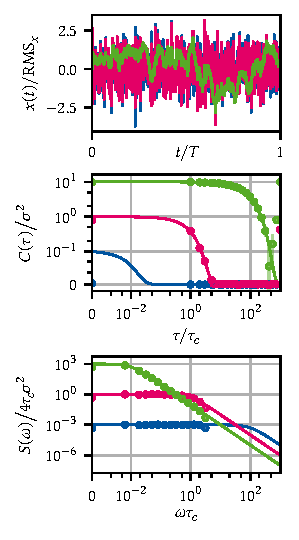
\includegraphics{img/pdf/spectrometer/lorentzian_psdcorr}
    \caption[\imgsource{img/py/spectrometer/lorentz.py}]{
        Ornstein-Uhlenbeck process.
        Simulated time traces (top), autocorrelation function (middle), \gls{psd} (bottom) of the Ornstein-Uhlenbeck process.
        Top: Simluated time traces using the algorithm presented in \cref{ch:ff:time_domain_methods}.
        The data are normalized to the computed \gls{rms} (equal to $\sigma$ in the continuous case).
        Middle: Theoretical autocorrelation function (\cref{eq:speck:ou:autocorrelation}, solid lines) and computed from the simulated data averaged over \num{e3} traces (circles, subset of points).
        Error bars indicate the standard error of the mean, axes are scaled with respect to the parameters of the magenta data, and data are plotted on an $\asinh$-scale.
        Bottom: Theoretical \gls{psd} (\cref{eq:speck:ou:psd}, solid lines) and periodograms computed from the simulated data using \code{scipy.signal.periodogram()}, \cf \cref{eq:speck:periodogram}, averaged over \num{e3} traces (circles, subset of points).
        Axes are again scaled with respect to the parameters of the magenta data and plotted on an $\asinh$-scale.
        Parameters are $\tau_c = \dt\times\{\num{e-2},\num{e0},\num{e2}\}$ and $\sigma^2=\sqrt{\tau_c}/4$ for blue, magenta, and green data, respectively.
    }
    \label{fig:speck:psdcorr}
\end{marginfigure}

To become familiar with the quantities $C(\tau)$ and $S(\omega)$, consider the Ornstein-Uhlenbeck process~\cite{Uhlenbeck1930}, the only stationary Gaussian Markovian stochastic process~\cite{VanKampen1976}.
The autocorrelation function of the Ornstein-Uhlenbeck process is given by
\begin{align}\label{eq:speck:ou:autocorrelation}
    C(\tau) = \sigma^2\e^{-\flatfrac{\tau}{\tau_c}},
\end{align}
with $\sigma$ the \gls{rms} and $\tau_c$ the correlation time of the process.
The \gls{psd} in turn is the Lorentzian function
\begin{align}\label{eq:speck:ou:psd}
    S(\omega) = \frac{2\sigma^2\tau_c}{1 + (\omega\tau_c)^2}.
\end{align}
For a given discretization time step \dt and hence bandwidth $\omega\in [0, \pi\fs]$, the Ornstein-Uhlenbeck process interpolates between perfectly uncorrelated, white noise ($\flatfrac{\dt}{\tau_c}\to\infty, S(\omega) = 2\tau_c\sigma^2$), correlated, Brownian noise ($\flatfrac{\dt}{\tau_c}\gg 1, S(\omega) = \flatfrac{2\sigma^2}{\tau_c\omega^2}$), and perfectly correlated, quasistatic noise ($\flatfrac{\dt}{\tau_c}\to 0, S(\omega) = \sigma^2\delta(\omega)$).
\Cref{fig:speck:psdcorr} depicts simulated data and its autocorrelation function and \gls{psd} for exemplary parameters: in the white noise limit ($\tau_c = \num{e-2}\dt$, blue), in the intermediate regime ($\tau_c = \dt$, magenta), and in the correlated regime ($\tau_c = \num{e+2}\dt$, green).
From the time series plot at the top it becomes clear that the \gls{rms} alone is insufficient to describe the properties of noisy signals as the curves differ significantly despite being normalized to their \gls{rms}.
The autocorrelation functions averaged over \num{e3} realizations of the noisy signals as well as their theoretical (continuous) value, \cref{eq:speck:ou:autocorrelation}, are plotted in the middle panel, normalized to $\tau_c=\dt$ and $\sigma^2=\flatfrac{\dt}{4}$.
For the white noise limit (blue), correlations are too short to be resolved with the given time discretization.
The correlations decay to $\e\inverse$ at $\flatfrac{\tau}{\tau_c}=\num{e-2},\num{e0},\num{e+2}$, respectively.
Finally, the bottom panel shows the \gls{psd}, \cref{eq:speck:ou:psd}, and its periodogram estimate, again averaged over \num{e3} realizations of the signal and normalized to $\tau_c=\dt$ and $\sigma^2=\flatfrac{\dt}{4}$.
The cross-over from white to Brownian \gls{psd} occurs at $\omega = \tau_c$.
While the simulated data for $\tau_c = \num{e-2}\dt$ appears perfectly white, that for $\tau_c = \num{e2}\dt$ appears perfectly \oneoverf-like because the spectrum is only white below the smallest resolvable frequency $\df = T\inverse$.

Having gotten an intuition for the quantities $C(\tau)$ and $S(\omega)$, let us move on to see how the latter may be obtained from time series data.
\Cref{eq:speck:psd:definition} represents the starting point for the experimental spectrum estimation procedure.
Instead of a continuous signal $x(t), t\in [0, T]$, consider its discretized version\sidenote{
    We only discuss the problem of equally spaced samples here.
    Variants for spectral estimation of time series with unequal spacing exist~\cite{Lomb1976,Scargle1982}.
}
\begin{align}\label{eq:speck:signal:discrete}
    x_n \qc n\in\lbrace 0, 1, \dotsc, N - 1\rbrace
\end{align}
defined at times $t_n = n\dt$ with $T = N\dt$ and where $\dt = \fs\inverse$ is the sampling interval (the inverse of the sampling frequency \fs).
Invoking the ergodic theorem,\sidenote{
    Note that the limit of perfectly correlated noise, $S(\omega)\propto\delta(\omega)$, technically does \emph{not} correspond to an ergodic process because $C(\tau)=\text{const.}\,\forall\tau\in(-\infty,\infty)$.
    In practice, this is always a mathematical idealization and the spectrum is actually better described by a nascent $\delta$-function with a small but finite width.
}
we can replace the long-term average in \cref{eq:speck:psd:definition} by the ensemble average over $M$ realizations of the noisy signal, $\left\lbrace x_n\gth{m}\right\rbrace_m$, and write
\begin{align}\label{eq:speck:psd:bartlett}
    S_n &= \frac{1}{M} \sum_{m=0}^{M-1} \abs{\hat{x}_n\gth{m}}^2 \\
        &= \frac{1}{M} \sum_{m=0}^{M-1} S_n\gth{m}
\end{align}
where $\hat{x}_n\gth{m}$ is the discrete Fourier transform of $x_n\gth{m}$, we defined the \emph{periodogram} of $x_n\gth{m}$ by
\begin{align}\label{eq:speck:periodogram}
    S_n\gth{m} = \abs{\hat{x}_n\gth{m}}^2,
\end{align}
and $S_n$ is an \emph{estimate} of the true \gls{psd} sampled at the discrete frequencies $\omega_n = \flatfrac{2\pi n}{T} \in 2\pi\times\lbrace\flatfrac{-\fs}{2}, \dotsc, \flatfrac{\fs}{2}\rbrace$.\sidenote{
    We blithely disregard integer algebra issues occuring here for conciseness and leave it as an exercise for the reader to figure out what the exact bounds of the set of $\omega_n$ are.
}
\Cref{eq:speck:psd:bartlett} is known as Bartlett's method~\cite{Bartlett1948} for spectrum estimation.\sidenote{
    \label{sidenote:continuum_limit}
    By taking the limit $M\to\infty$ one recovers the true \gls{psd}, \[\lim_{M\to\infty}S_n = S(\omega_n).\]
    The continuum limit is as always obtained by sending $\dt\to 0, N\to\infty, N\dt=\text{const}$.
}

To better understand the properties of this estimate, let us take a look at the parameters $\dt$, $N$, and $M$.
The sampling interval $\dt$ defines the largest resolvable frequency by the Nyquist sampling theorem,
\begin{align}\label{eq:speck:f_max}
    \fmax = \frac{\fs}{2} = \frac{1}{2\dt}.
\end{align}
In turn, the number of samples $N$ determines the frequency resolution $\df$, or smallest resolvable frequency,
\begin{align}\label{eq:speck:f_min}
    \fmin = \df = \frac{1}{T} = \frac{1}{N\dt} = \frac{\fs}{N}.
\end{align}
Lastly, $M$ determines the variance of the set of periodograms $\bigl\lbrace S_n\gth{m}\bigr\rbrace_{i=0}^{M-1}$ and hence the accuracy of the estimate $S_n$.

In practice, the ensemble realizations $i$ are of course obtained sequentially, implying that one acquires a time series of data $x_n, n\in\lbrace0, 1, \dotsc, NM - 1\rbrace$ and partitions these data into $M$ sequences of length $N$.
It becomes clear, then, that the Bartlett average (\cref{eq:speck:psd:bartlett}) trades spectral resolution (larger $N$) for estimation accuracy (larger $M$) given the finite acquisition time $T = NM\dt$.

An improvement in data efficiency can be achieved using Welch's method~\cite{Welch1967}.
To see how, we first need to discuss spectral windowing.

\section{Window functions}\label{sec:speck:theory:windows}
Partitioning a signal $x_n$ into $M$ sections $x_n\gth{m}$ of length $N$ is mathematically equivalent to multiplying the signal with the rectangular \emph{window function} given by\sidenote{
    This window is also known as the boxcar or Dirichlet window.
}
\begin{align}\label{eq:speck:window:boxcar}
    w_n\gth{m} =
    \begin{dcases}
        1 &\qif* (m - 1) N \leq n < m N\qand \\
        0 &\qelse*
    \end{dcases}
\end{align}
so that $x_n\gth{m} = x_n w_n\gth{m}$.
Now recall that multiplication and convolution are duals under the Fourier transform, implying that
\begin{align}\label{eq:speck:window:ft_pairs}
    \hat{x}_n\gth{m} = \hat{x}_n \ast \hat{w}_n\gth{m},
\end{align}
where the Fourier representation of the rectangular window\sidenote{
    $\sinc(x) = \flatfrac{\sin(x)}{x}$.
}
\begin{align}
    \hat{w}_n\gth{m} &= \hat{w}_n \e^{-\i(m - \flatfrac{1}{2})\omega_n T}, \label{eq:speck:window:boxcar:fourier}\\
             \hat{w}_n &= T\sinc\left(\frac{\omega_n T}{2}\right). \label{eq:speck:window:boxcar:fourier:unshifted}
\end{align}
\Cref{fig:speck:boxcar_fourier} shows the unshifted rectangular window $\hat{w}_n$ in Fourier space.
We can hence understand the Fourier spectrum of $x_n\gth{m}$ as sampling $\hat{x}_n$ with the probe $\hat{w}_n\gth{m}$.
However, whereas in the continuum limit (see \cref{sidenote:continuum_limit}) \cref{eq:speck:window:boxcar:fourier:unshifted} tends towards $\delta(\omega_n)$ and thus will produce a faithful reconstruction of the true spectrum, the finite sample rate $\fs$ of discrete signals and observation length $T$ induce finite frequency sampling and bandwidth of the probe as well as \emph{sidelobes}.\sidenote{
    For the optically inclined: this is akin to Fraunhofer diffraction at an aperture.
}
These effects incur what is known as \emph{spectral leakage} and \emph{scalloping loss}, respectively, and lead to artifacts and deviations of the spectrum estimator $S_n$ from the true spectrum $S(\omega_n)$~\cite{Harris1978,Koopmans1995}.

\begin{marginfigure}
    \centering
    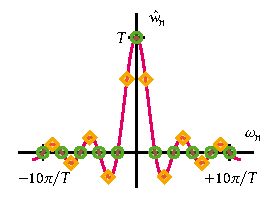
\includegraphics{img/pdf/spectrometer/rect}
    \caption[\imgsource{img/py/spectrometer/pyspeck.py}]{
        The Fourier representation of the rectangular window in continuous time (solid line) and for discrete frequencies $\omega_n = \flatfrac{2\pi n}{T}$ (circles).
        Introducing a phase shift, that is, shifting the window with respect to the signal in time, effectively shifts $\omega_n \to \omega_{n+\eta}$ as indicated for $\eta=\flatfrac{1}{2}$ (diamonds).
        This incurs scalloping loss.
    }
    \label{fig:speck:boxcar_fourier}
\end{marginfigure}

For this reason, a plethora of \emph{window functions} have been introduced to mitigate the effects of spectral leakage.
Key properties of a window are the spectral bandwidth (center lobe width) and sidelobe amplitude between which there typically is a tradeoff.\sidenote{
    Wikipedia gives a good overview of existing window functions~\cite{WindowFunctionWiki}.
}
A window frequently used in spectral analysis is the Hann window~\cite{Nuttall1981},
\begin{align}\label{eq:speck:window:hann}
    w_n\gth{m} =
    \begin{dcases}
        \sin^2\left(\frac{\pi n}{N}\right) &\qif* (m - 1)N\leq n < mN\qand \\
        0 &\text{else},
    \end{dcases}
\end{align}
with the Fourier representation of the unshifted window,
\begin{align}\label{eq:speck:window:hann:fourier_unshifted}
    \hat{w}_n &= \frac{T}{2}\sinc\left(\frac{\omega_n T}{2}\right)
                 %  \frac{1}{2(1 - \flatfrac{\omega_n T}{2\pi})(1 + \flatfrac{\omega_n T}{2\pi})},
                    \frac{1}{1 - \left(\flatfrac{\omega_n T}{2\pi}\right)^2}
\end{align}
shown in \cref{fig:speck:hann_fourier}.
The favorable properties of the Hann window are apparent when compared to the rectangular window in \cref{eq:speck:window:boxcar:fourier:unshifted} and \cref{fig:speck:boxcar_fourier}; the sidelobes are quadratically suppressed while the center lobe is broadened by a factor of two.

\begin{marginfigure}
    \centering
    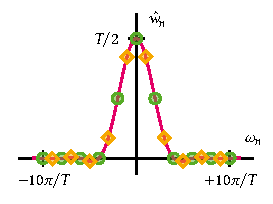
\includegraphics{img/pdf/spectrometer/hann}
    \caption[\imgsource{img/py/spectrometer/pyspeck.py}]{
        The Fourier representation of the Hann window in continuous time (solid line) and for discrete frequencies $\omega_n$ (circles).
        Diamonds indicate discrete sampling when the window completely out of phase with the signal (\cf \cref{fig:speck:boxcar_fourier}).
    }
    \label{fig:speck:hann_fourier}
\end{marginfigure}

Another favorable property of the Hann window is that $w_0\gth{0} = w_{N-1}\gth{0} = 0$.
This suppresses detrimental effects arising from a possible discontinuity ($x_0\gth{0}\neq x_{N-1}\gth{0}$) at the edge of a data segment related to the discrete Fourier transform, which assumes periodic data.\sidenote{
    Although this can usually also be achieved approximately by detrending the data before performing the Fourier transform, which is a good idea in any case.
}

\section{Welch's method}\label{sec:speck:theory:welch}
Contemplating \cref{eq:speck:window:hann}, one might come to the conclusion that using a window such as this is not very data efficient in the sense that a large fraction of samples located at the edge of the window is strongly suppressed and hence does not contribute significantly to the spectrum estimate.
To alleviate this lack of efficiency, one can introduce an overlap between adjacent data windows.
That is, instead of partitioning the data $x_n$ into $M$ non-overlapping sections of length $N$, one shifts the $m$th window forward by $-mK$ with $K>0$ the overlap.
Finally, the periodogram (\cref{eq:speck:periodogram}) is computed for each window and subsequently averaged to obtain the spectrum estimator (\cref{eq:speck:psd:bartlett}).

This method of spectrum estimation is known as Welch's method~\cite{Welch1967}.
One can show~\cite{Welch1967} that the correlation between the periodograms of adjacent, overlapping windows is sufficiently small to avoid a biased estimate.
The overlap naturally depends on the choice of window; a typical value for the Hann window $K = \flatfrac{N}{2}$ with which one would obtain $M = \flatfrac{2L}{N} - 1$ windows for data of length $L$.\sidenote{
    Again neglecting integer arithmetic issues.
}
\begin{figure}
    \centering
    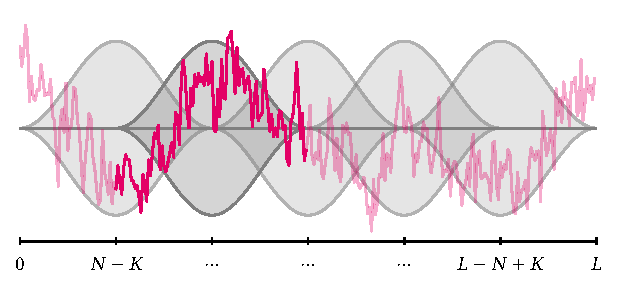
\includegraphics[width=\textwidth]{img/pdf/spectrometer/welch}
    \caption[\imgsource{img/py/spectrometer/pyspeck.py}]{
        Illustration of Welch's method for spectrum estimation.
        The data (magenta) of length $L$ is partitioned into $K = \flatfrac{2L}{N} - 1$ segments of length $N$.
        Each segment is multiplied with a window function (gray) which reduces spectral leakage and other artifacts.
        A finite overlap $K$ between adjacent windows (gray) ensures efficient sample use.
    }
    \label{fig:speck:welch}
\end{figure}

\Cref{fig:speck:welch} conceptually illustrates Welch's method for a trace of \oneoverf noise with $L = 300$ samples in total.
Choosing the Hann window and an overlap of \qty{50}{\percent} results in $M=5$ segments for a window length of $N=100$.
The data in the second window is highlighted.

\section{Parameters \& Properties of the \acrshort{psd}}\label{sec:speck:theory:welch:parameters}
\begin{margintable}[*-7]
    \centering
    \footnotesize
    \caption[Overview of spectrum estimation parameters]{
        Overview of spectrum estimation parameters.
        The parameters can be assigned into four groups
        \begin{enumerate*}[
            before=\unskip{: }, itemjoin={{, }}, itemjoin*={{, and }}
        ]
            \item \acrshort{daq} parameters configuring the \acrlong{daq} device
            \item Welch parameters specifying the periodogram averaging
            \item Spectrum properties induced by the above
            \item External parameters unrelated to the others
        \end{enumerate*}.
    }
    \label{tab:speck:theory:parameters}
    \renewcommand{\arraystretch}{1.1}
    \begin{tabularx}{\marginparwidth}{ c l }
        \multicolumn{2}{l}{\textsc{1. \acrshort{daq} parameters}} \\
        \toprule
        $L$ & Total number of samples \\
        \fs & Sample rate \\
        [0.5ex]
        \multicolumn{2}{l}{\textsc{2. Welch parameters}} \\
        \toprule
        $K$ & Number of overlap samples \\
        $N$ & Number of segment samples \\
        $M$ & Number of Welch segments \\
        [0.5ex]
        \multicolumn{2}{l}{\textsc{3. Spectrum parameters}} \\
        \toprule
        \fmin & Smallest resolvable frequency \\
        \fmax & Largest resolvable frequency \\
        [0.5ex]
        \multicolumn{2}{l}{\textsc{4. Miscellaneous parameters}} \\
        \toprule
        $O$ & Number of outer averages \\
    \end{tabularx}
\end{margintable}
We are now in a position to discuss how the various parameters of a time series relate to both the physical parameters of the resulting spectrum estimate and to each other.
To this end, we will go through the typical procedure of acquiring a spectrum estimate using Welch's method chronologically.

To acquire data using some form of (digital) \gls{daq}, one usually needs to specify two parameters first: the total number of samples to be acquired, $L$, and the sample rate \fs.
This results in a measurement of duration $T = L\dt$ where $\dt = \fs\inverse$ as previously mentioned.
The choice of \fs already induces an upper bound on the first parameter characterizing the \gls{psd} estimate: the largest resolvable frequency $\fmax\leq\flatfrac{\fs}{2}$ (\cf \cref{eq:speck:f_max}, but note that we allow \fmax to be smaller than half the sample rate in anticipation of hardware constraints).
Next, we choose a number of Welch averages, $M$, \ie, data partitions, and their overlap, $K$.
In doing so, one fixes the number of samples per partition $N$ and thereby induces the lower bound on the second parameter characterizing the \gls{psd} estimate: the frequency spacing $\df = \flatfrac{1}{N} \leq \fmin$ (\cf \cref{eq:speck:f_min}).\sidenote[][*-3]{
    Technically, the smallest resolvable frequency in a \gls{fft} is zero, of course. But as data is typically detrended (a constant or linear trend subtracted) before computation of the periodogram, the smallest \emph{meaningful} frequency is given by \fmin.
}
% TODO: be consistent in use of segment vs partition?
Finally, we can introduce a number of \emph{outer} averages $O$, that is, the number of data batches that are acquired.
While not directly related to Welch's method, choosing $O > 1$ can, for instance, help achieve a certain variance if the number of samples per batch, $L$, is limited by the \acrlong{daq} hardware, or simply allow for updating the spectrum estimate as data is being acquired.
\Cref{fig:speck:theory:parameters} shows the relationships of the various parameters among each other.
In \cref{subsec:speck:software:design:daq}, I lay out how these inter-dependencies are implemented in software.

\begin{figure}
    \centering
    \begin{tikzpicture}[
    >=stealth,
    auto,
    box/.style={
        draw,
        rectangle,
        rounded corners,
        thick,
        align=center,
        inner sep=2mm,
%        drop shadow,
    },
    float1/.style={box, fill=RWTHmagenta25, text=RWTHmagenta100},
    float2/.style={box, fill=RWTHmagenta10, text=RWTHmagenta75},
    int1/.style={box, fill=RWTHgreen25, text=RWTHgreen100},
    int2/.style={box, fill=RWTHgreen10, text=RWTHgreen75},
    int3/.style={box, fill=RWTHblack10, text=RWTHblack100},
]

    % Central node: nperseg
    \node[int1] (nperseg) {$N$};

    % Frequency branch: relative to nperseg, all nodes placed at the same x-coordinate.
    \node[float1, above left=1cm of nperseg, anchor=center] (fs) {\fs};
    \node[float1, below left=1cm of nperseg, anchor=center] (df) {\df};
    \node[float2, left=of fs] (fmax) {\fmax};
    \node[float2, left=of df] (fmin) {\fmin};

    % Segmentation branch: relative to nperseg
    \node[int2, right=of nperseg] (npts) {$L$};
    \node[int2, above right=of npts, anchor=center] (noverlap) {$K$};
    \node[int2, below right=of npts, anchor=center] (nseg) {$M$};

    % Stand-alone node for n_avg
    \node[int3, above=1cm of $(npts)!0.5!(nperseg)$] (navg) {$O$};

    % Draw frequency branch arrows
    \draw[->] (nperseg) -- (fs);
    \draw[->] (nperseg) -- (df);
    \draw[<->] (df) to[bend left=45] (fs);
    \draw[->] (fs) to[bend right=45] (fmax);
    \draw[->] (df) to[bend left=45] (fmin);
    \draw[<->] (fs) -- (nperseg);
    \draw[<->] (df) -- (nperseg);

    % Draw segmentation branch arrows (nperseg, noverlap, and n_seg together inform n_pts)
    \draw[<->] (nperseg) -- (npts);
    \draw[->] (noverlap) -- (npts);
    \draw[->] (nseg) -- (npts);

    % n_avg remains independent (no arrows drawn)

\end{tikzpicture}

    \caption[\imgsource{img/tikz/spectrometer/daq_settings.tex}]{
        Relationships of data acquisition parameters (\cf \cref{tab:speck:theory:parameters,tab:speck:software:parameters}, with arrows indicating dependencies.
        $N$, \fs, and \df are the central quantities defining the estimated spectrum's properties.
        From \fs and \df follow (bounds for) \fmax and \fmin.
        From $N$, together with $K$ and $M$, follows $L$, the total number of samples per data batch.
    }
    \label{fig:speck:theory:parameters}
\end{figure}

To conclude this chapter, let us discuss some of the properties of stochastic processes and their autocorrelation function and \gls{psd}.
Consider again the process $x(t)$.
We say $x(t)$ is \emph{Gaussian} if $x(t)\sim\mathcal{N}(\mu, \sigma^2)\,\forall t$, meaning that the value of $x(t)$ at a given point in time follows a normal distribution with some mean $\mu$ and variance $\sigma^2$ over multiple realizations of the process.
In this case, its statistical properties are fully described by the autocorrelation function $C(\tau)$ and \gls{psd} $S(\omega)$.
This is because only the first two cumulants of a Gaussian distribution are nonzero~\cite{Fox1978}.
For the purpose of noise estimation, the assumption of Gaussianity is a rather weak one as the noise typically arises from a large ensemble of individual fluctuators and is therefore well approximated by a Gaussian distribution by the central limit theorem~\cite{Krzywda2020}.\sidenote{
    As an example, consider electronic devices, where voltage noise is thought to arise from a large number of defects and other charge traps in oxides being populated and depopulated at certain rates $\gamma$. The ensemble average over these so-called \glspl{tlf} then yields the well-known \oneoverf-like noise spectra~\cite{Schriefl2006,Beaudoin2015} (at least for a large density~\cite{Mehmandoost2024}).
}
Even if $x(t)$ is not perfectly Gaussian, non-Gaussian contributions can be seen as higher-order contributions if viewed from the perspective of perturbation theory, and therefore the \gls{psd} still captures a significant part of the statistical properties.
For this reason, the \gls{psd} is the central quantity of interest in noise spectroscopy.
Let us just note at this point that techniques to estimate higher-order spectra (or \emph{polyspectra}) exist~\cite{Chandran1994,Norris2016,Szankowski2017}.

For real signals $x(t)\in\mathbb{R}$, the autocorrelation function $C(\tau)$ is an even function, while for $x(t)\in\mathbb{C}$ its real part is even and its complex part odd.
From this it immediately follows that for real $x(t)$ $S(\omega)$ is also an even function and one therefore distinguishes the \emph{two-sided} \gls{psd} $S^{(2)}(\omega)$ defined over $\mathbb{R}$ from the \emph{one-sided} \gls{psd} $S^{(1)}(\omega) = 2 S^{(2)}(\omega)$ defined only over $\mathbb{R}^+$.
Complex $x(t)$ such as those generated by \glspl{lia} after demodulation in turn have asymmetric, two-sided \glspl{psd}.
In this chapter so far, we have implicitly employed the two-sided definition, but in the software package presented in \cref{ch:speck:software}, two-sided spectra are used only for complex data since they contain redundant information for real data.

% mainfile: ../../main.tex
\chapter{The \pyspeck software package}\label{ch:speck:software}
\mylettrine{I}{n} this chapter, I introduce the \pyspeck \python package\sidenote{
    The package repository is hosted on \href{https://git.rwth-aachen.de/qutech/python-spectrometer/}{GitLab}.
    Its documentation is automatically generated and hosted on \href{https://qutech.pages.rwth-aachen.de/python-spectrometer/}{GitLab Pages}.
    Releases are automatically published to \href{https://pypi.org/project/python-spectrometer/}{PyPI} and allow the package to be installed using \code{pip install python-spectrometer}.
}
and lay out its design and functionality.
This software package was developed to make it easier for experimentalists to transfer the mathematical machinery introduced in \cref{ch:speck:theory} to the lab.
While in principle the entire process of spectrum estimation from a given array of time series data is already covered by the \code{welch()} routine in \scipy~\sidecite{WelchScipy}, obtaining the data array is not standardized.
Different \gls{daq} instruments have different capabilities, both on the hardware and the software level, and different driver interfaces to communicate with them.
This implies custom \acrlong{daq} code is required for every instrument, introducing a significant entry barrier to spectral analysis.
The \pyspeck package implements a simple interface to different hardware instruments that allows for changing the hardware backend without having to adapt the user-facing code and also incorporates different hardware constraints.

What is more, noise spectroscopy tends to be a visual endeavor in practice; it is hard to compare different noise spectra based on quantitative reasoning alone.
Data visualization is hence an integral part of noise spectroscopy, but plotting is not just plotting.
Do we want the data to be shown on a log-log scale?\sidenote{
    The short answer is yes, but it comes with visual side-effects that demand other ways of plotting data at times.
    The long answer is therefore yes, \emph{and} \dots
}
Do we want to show the relative magnitude of different data sets?
Do we want to inspect the time traces as well?
The \pyspeck package addresses these questions by allowing users to interactively change features of the main plot window to adapt it to the form best suited to the situation at hand.

Moreover, when concerned with noise spectrum estimation, we are typically more interested in specifying parameters of the resulting \gls{psd} rather than parameters of the underlying time series data.
The \pyspeck package approaches \acrlong{daq} from the inverse direction: rather than inferring the spectrum properties from the time series data, users specify the properties they would like the resulting spectrum to have and the package chooses the correct parameters for \acrlong{daq} accordingly.

\section{Package design and implementation}\label{sec:speck:software:design}
\begin{marginfigure}[-3.75cm]
    \forestset{
    dir tree/.style={
        for tree={
            parent anchor=south west,
            child anchor=west,
            anchor=mid west,
            inner ysep=0pt,
            grow'=0,
            align=left,
            s sep=1ex,
            edge path={
                \noexpand\path [draw, \forestoption{edge}] (!u.parent anchor) ++(0.75em,0) |- (.child anchor)\forestoption{edge label};
            },
            font=\footnotesize\ttfamily,
            if n children=0{}{
                delay={
                    prepend={[,phantom, calign with current]}
                }
            },
            fit=band,
            before computing xy={
                l=1.5em
            }
        },
    }
}
\begin{forest}
    dir tree
    [
        [{\faIcon[regular]{folder} \pyspeckpath{doc}{doc}}]
        [{\faIcon[regular]{folder-open} \pyspeckpath{src}{src}}
            [{\faIcon[regular]{folder-open} \pyspeckpath{src/python_spectrometer}{python\_spectrometer}}
                [{\faIcon[regular]{folder-open} \pyspeckpath{src/python_spectrometer/daq}{daq}}
                    [{\faIcon[regular]{file-code} \pyspeckpath{src/python_spectrometer/daq/__init__.py}{\_\_init\_\_.py}}]
                    [{\faIcon[regular]{file-code} \pyspeckpath{src/python_spectrometer/daq/base.py}{base.py}}]
                    [{\faIcon[regular]{file-code} \pyspeckpath{src/python_spectrometer/daq/qcodes.py}{qcodes.py}}]
                    [{\faIcon[regular]{file-code} \pyspeckpath{src/python_spectrometer/daq/settings.py}{settings.py}}]
                    [{\faIcon[regular]{file-code} \ldots}]
                ]
                [{\faIcon[regular]{file-code} \pyspeckpath{src/python_spectrometer/__init__.py}{\_\_init\_\_.py}}]
                [{\faIcon[regular]{file-code} \pyspeckpath{src/python_spectrometer/_audio_manager.py}{\_audio\_manager.py}}]
                [{\faIcon[regular]{file-code} \pyspeckpath{src/python_spectrometer/_plot_manager.py}{\_plot\_manager.py}}]
                [{\faIcon[regular]{file-code} \pyspeckpath{src/python_spectrometer/core.py}{core.py}}]
            ]
        ]
        [{\faIcon[regular]{folder} \pyspeckpath{tests}{tests}}]
        [{\faIcon[regular]{file-code} \pyspeckpath{pyproject.toml}{pyproject.toml}}]
        [{\faIcon[regular]{file-code} \ldots}]
    ]
\end{forest}

    \caption[Source tree structure of the \pyspeck package.]{
        Source tree structure of the \pyspeck package.
        Driver wrappers are placed in the \code{daq} subpackage.
        \code{core.py} exports the \code{Spectrometer} class.
    }
    \label{fig:speck:software:tree}
\end{marginfigure}
The \pyspeck package provides a central class, \code{Spectrometer}, that users interact with to perform data acquisition, spectrum estimation, and plotting.
It is instantiated with an instance of a child class of the \code{DAQ} base class that implements an interface to various \gls{daq} hardware devices.\sidenote[][4.6cm]{
    Actually \emph{drivers} to be more precise.
}
New spectra are obtained by calling the \code{Spectrometer.take()} method with all acquisition and metadata settings.
In the following, I will go over the the design of these aspects of the package in more detail.

\subsection{Data acquisition}\label{subsec:speck:software:design:daq}
\Cref{fig:speck:software:tree} shows the directory structure of the source code.
The \code{daq} subpackage contains on the one hand the declaration of the \code{DAQ} abstract base class (\code{base.py}) and its child class implementations (\code{qcodes.py}, \etc), and on the other the \code{settings.py} module, which defines the \code{DAQSettings} class.
This class is used in the background to validate data acquisition settings both for consistency (see \cref{subsec:speck:theory:welch:parameters}) and hardware constraints.

\begin{margintable}
    \footnotesize
    \centering
    \setmintedinline[Python]{fontsize=\footnotesize}
    \caption[Overview of spectrum estimation parameters]{
        Variable names used in \cref{ch:speck:theory} and their corresponding parameter names as used in \pyspeck and \code{scipy.signal.welch()}~\cite{WelchScipy}.
    }
    \label{tab:speck:software:parameters}
    \begin{tabular}{ c C }
        \toprule
        Variable & Parameter \\
        \midrule
        $L$ & n_pts \\
        $N$ & nperseg \\
        $K$ & noverlap \\
        $M$ & n_seg \\
        $O$ & n_avg \\
        \fs & fs \\
        \fmax & f_max \\
        \fmin & f_min \\
        \bottomrule
    \end{tabular}
\end{margintable}

To better understand the necessity of this functionality, consider the typical scenario of a physicist\sidenote{
    Let's call her Alice.
}
in the lab.
Alice has wired up her experiment, performed a first measurement, and to her dismay discovered that the data is too noisy to see the sought-after effect.
She sets up the \pyspeck code to investigate the noise spectrum of her measurement setup.
From her noisy data she could already estimate the frequency of the most harrowing noise, so she knows the frequency band $[\fmin, \fmax]$ she is most interested in.
But because she is lazy,\sidenote{
    Physicists generally are.
}
she does not want to do the mental gymnastics to convert \fmin to the parameter that her \gls{daq} device understands, $L$ (see \cref{tab:speck:software:parameters}), especially considering that $L$ depends on the number of Welch averages and the overlap.
Furthermore, while she could just about do the conversion from \fmax to the other relevant \gls{daq} parameter, \fs, in her head, her device imposes hardware constraints on the allowed sample rates she can select!
The \code{DAQSettings} class addresses these issues.
It is instantiated with any subset of the parameters listed in \cref{tab:speck:software:parameters}\sidenote{
    \code{DAQSettings} inherits from the builtin \code{dict} and as such can contain arbitrary other keys besides those listed in \cref{tab:speck:software:parameters}.
    However, automatic validation of parameter consistency is only performed for these special keys.
}
and attempts to resolve the parameter interdependencies lined out in \cref{subsec:speck:theory:welch:parameters} upon calling \code{DAQSettings.to_consistent_dict()}.\sidenote{
    Since the graph spanned by the parameters is not acyclic, this only works \emph{most} of the time.
}
This either infers those parameters that were not given from those that were or, if not possible, uses a default value.
Child classes of the \code{DAQ} class can subclass \code{DAQSettings} to implement hardware constraints such as a finite set of allowed sampling rates or a maximum number of samples per data buffer.

For instance, Alice might want to measure the noise spectrum in the frequency band $[\qty{1.5}{\hertz}, \qty{72}{\kilo\hertz}]$.
Although she would not have to do this explicitly,\sidenote{
    Settings are automatically parsed when passed to the \code{take()} method of the \code{Spectrometer} class.
}
she could inspect the parameters after resolution using the code shown in \cref{lst:speck:daq:settings}.

\begin{listing}[htpb]
    \begin{py}
        >>> from python_spectrometer.daq import DAQSettings
        >>> settings = DAQSettings(f_min=1.5, f_max=7.2e4)
        >>> settings.to_consistent_dict()
        {'f_min': 1.5,
         'f_max': 72000.0,
         'fs': 144000.0,
         'df': 1.5,
         'nperseg': 96000,
         'noverlap': 48000,
         'n_seg': 5,
         'n_pts': 288000,
         'n_avg': 1}
    \end{py}
    \caption{
        \code{DAQSettings} example showcasing automatic parameter resolution.
        \code{n_avg} determines the number of outer averages, \ie, the number of data buffers acquired and processed individually.
    }
    \label{lst:speck:daq:settings}
\end{listing}

\begin{marginlisting}[-2.5cm]
    \begin{py}[fontsize=\footnotesize]
    {'f_min': 14.30511474609375,
     'f_max': 72000.0,
     'fs': 234375.0,
     'df': 14.30511474609375,
     'nperseg': 16384,
     'noverlap': 0,
     'n_seg': 1,
     'n_pts': 16384,
     'n_avg': 1}
    \end{py}
    \caption[Resolved \code{DAQSettings} for MFLI Scope]{
        Resolved settings for the same input parameters as in \cref{lst:speck:daq:settings} but for the \code{ZurichInstrumentsMFLIScope} backend with hardware constraints on \code{n_pts} and \code{fs}.
    }
    \label{lst:speck:daq:settings:mfli_scope}
\end{marginlisting}

If the instrument she'd chosen for data acquisition had been a Zurich Instruments MFLI's Scope module,\sidenote[][2.7cm]{
    \url{https://docs.zhinst.com/labone_api_user_manual/modules/scope/index.html}
}
the same requested settings would have resolved to those shown in \cref{lst:speck:daq:settings:mfli_scope}.\sidenote[][3.5cm]{
    And issued a warning to inform the user their requested settings could not be matched.
}
This is because the Scope module constrains $L\in[2^{12},2^{14}]$ and $\fs\in\qty{60}{\mega\hertz}\times 2^{[-16, 0]} \approx \allowbreak \lbrace \qty{915.5}{\hertz}, \allowbreak \dotsc, \allowbreak \qty{30}{\mega\hertz}, \qty{60}{\mega\hertz}\rbrace$.

As already mentioned, the \code{DAQ} base class implements a common interface for different hardware backends, allowing the \code{Spectrometer} class to be hardware agnostic.
That is, changing the instrument that is used to acquire the data does not necessitate adapting the code used to interact with the \code{Spectrometer}.
To enable this, different instruments require small wrapper drivers that map the functionality of their actual driver onto the interface dictated by the \code{DAQ} class.
This is achieved by subclassing \code{DAQ} and implementing the \code{DAQ.setup()} and \code{DAQ.acquire()} methods.
Their functionality is best illustrated by the internal workflow as representatively shown in \cref{lst:speck:daq:workflow}.

\begin{listing}[htpb]
    \begin{py}
        daq = MyDAQ(driver_handle)

        parsed_settings = daq.setup(**user_settings)
        acquisition_generator = daq.acquire(**parsed_settings)

        for data_buffer in acquisition_generator:
            estimate_psd(data_buffer)
    \end{py}
    \caption[\gls{daq} workflow pseudocode]{
        \gls{daq} workflow pseudocode.
        A \code{MyDAQ} object (representing the instrument \code{My}) is instantiated with a driver object (for instance a \href{https://github.com/microsoft/qcodes}{QCoDeS} \code{Instrument}).
        The instrument is configured with the given \code{user_settings}.
        Calling the generator function \code{daq.acquire()} with the actual device settings returns a generator, iterating over which yields one data buffer per iteration.
        The data buffers can then be passed to further processing functions (the \gls{psd} estimator in our example).
    }
    \label{lst:speck:daq:workflow}
\end{listing}

When acquiring a new spectrum, all settings supplied by the user are first fed into the \code{setup()} method where instrument configuration takes place.
The method returns the actual device settings,\sidenote{
    Which might differ from the requested settings as outlined above.
}
which are then forwarded to the \code{acquire()} generator function.
Here, the instrument is armed (if necessary), and subsequently data is fetched from the device and yielded to the caller \code{n_avg} times, where \code{n_avg} is the number of outer averages.\sidenote{
    \Ie, the number of time series data batches acquired, as opposed to the number of Welch averages \code{n_seg} within one batch.
}
An exemplary implementation of a \code{DAQ} subclass for a fictitious instrument is shown in \cref{lst:speck:daq:pseudocode}.
In addition to the methods to configure the instrument and perform data acquisition, it is possible to override the \code{DAQSettings} property to implement instrument-specific hardware constraints such as, in this example, the number of samples per buffer being constrained to the discrete interval $[1, 2048]$.
Leveraging the \code{qutil.domains} module, more complex constraints such as sample rates restricted to an internal clock rate divided by a power of two\sidenote{
    See for example the implementation of the \href{https://git.rwth-aachen.de/qutech/python-spectrometer/-/blob/main/src/python_spectrometer/daq/atsaverage.py}{AlazarTech ATS9440} digitizer card.
}
can be specified.

\begin{listing}
    \begin{py}
        # daq/mydaq.py
        import dataclasses
        from qutil.domains import DiscreteInterval
        from .base import DAQ
        from .settings import DAQSettings

        @dataclasses.dataclass
        class MyDAQ(DAQ):
            handle: mydriver.DeviceHandle

            @property
            def DAQSettings(self) -> type[DAQSettings]:
                class MyDAQSettings(DAQSettings):
                    ALLOWED_NPERSEG = DiscreteInterval(1, 2048)
                return MyDAQSettings

            def setup(self, **settings) -> dict:
                settings = self.DAQSettings(settings)
                parsed_settings = settings.to_consistent_dict()
                self.handle.configure(parsed_settings)
                return parsed_settings

            def acquire(self, n_avg: int, *, **settings) -> Generator:
                self.handle.arm(n_avg)
                for _ in range(n_avg):
                    self.handle.wait_for_trigger()
                    yield self.handle.fetch()
                return self.handle.metadata
    \end{py}
    \caption[\code{DAQ} pseudocode]{
        Exemplary code for a \code{DAQ} implementation of some instrument with given driver class \code{DeviceHandle} in the package \code{mydriver}.
        The \code{MyDAQ} class is instantiated with a \code{DeviceHandle} instance.
        Optionally, the \code{DAQSettings} property can be overridden to implement hardware constraints or default values for data acquisition parameters.
        For this, the \code{qutil.domains} module provides several classes that represent bounded domains and sets.
        The \code{setup()} method parses the given acquisition settings and configures the instrument through the external driver interface \code{handle.configure()}.
        The \code{acquire()} method arms the instrument (if necessary) and loops over the number of outer averages, \code{n_avg}.
        In the body of the loop, it can wait for external triggers (or send software triggers) before yielding a batch of data fetched from the external driver interface.
        Once acquisition is done, the method can return arbitrary metadata to the \code{Spectrometer} object to attach to the stored data.
    }
    \label{lst:speck:daq:pseudocode}
\end{listing}

\subsection{Data processing}\label{subsec:speck:software:design:processing}
Once time series data has been acquired using a given \code{DAQ} backend, it could in principle immediately be used to estimate the \gls{psd} following \cref{eq:speck:psd:bartlett}.
However, it is often desirable to transform, or process, the data in some fashion.
This can include simple transformations such as accounting for the gain of a \gls{tia} and convert the voltage back to a current,\sidenote{
    Although it is of course less than trivial to discriminate between current and voltage noise in a \gls{tia}.
}
or more complex ones such as applying calibrations.
In particular, since the process of computing the \gls{psd} already involves Fourier transformation, the processing can also be performed in frequency space.

In \pyspeck, this can be done using a \code{procfn} (in the time domain) or \code{fourier_procfn} (in the Fourier domain).
The former is specified as an argument directly to the \code{Spectrometer} constructor.
It is a callable with signature \code{(x, **kwargs) -> xp}, that is, takes the time series data as its first (positional) argument and arbitrary settings that are passed through from the \code{take()} method as keyword arguments, and returns the processed data.
\Cref{lst:speck:procfn} shows a simple function that accounts for the gain of an amplifier.
The latter is specified in the \code{psd_estimator} argument of the \code{Spectrometer} constructor.
This argument allows the user to specify a custom estimator for the \gls{psd}, in which case a callable is expected.
Otherwise, it should be a mapping containing parameters for the default \gls{psd} estimator, \code{scipy.signal.welch()}~\sidecite{WelchScipy}.
Here, the keyword \code{fourier_procfn} should be a callable with signature \code{(xf, f, **kwargs) -> (xfp, fp)}.\sidenote{
    \Ie, the \code{psd_estimator} argument would be \code{{"fourier_procfn": fn}}.
}
That is, it should take the frequency-space data, the corresponding frequencies, and arbitrary keyword arguments and return a tuple of the processed data and the corresponding frequencies.

\begin{marginlisting}
    \begin{py}[fontsize=\footnotesize]
        def comp_gain(x, gain=1.0, **_):
            return x / gain
    \end{py}
    \caption[Simple \code{procfn} example]{
        A simple \code{procfn}, which converts amplified data back to the level before amplification.
        Note the token \code{**_} variable keyword argument that ensures no errors arise from other parameters being passed to the function.
        More complex processing chains can concisely be defined with \code{qutil.functools.FunctionChain} that pipes the output of one function into the input of the next.
    }
    \label{lst:speck:procfn}
\end{marginlisting}

The latter are required in case the function modifies the frequencies.\sidenote{
    One example is the \code{octave_band_rms()} function from the \code{qutil.signal_processing} subpackage~\cite{OctaveBandRmsQutil} that decimates frequencies to fractions of octave bands. See \cref{part:setup} for a use-case. TODO: ref
}
A simple example for a processing function in Fourier space is shown in \cref{lst:speck:fourier_procfn}, which computes the \mbox{(anti-)}derivative of the data using the fact that
\begin{marginlisting}
    \begin{py}[fontsize=\footnotesize]
        def derivative(xf, f, n=0, **_):
            return xf / (2j * pi * f)**n
    \end{py}
    \caption[Simple \code{fourier_procfn} example]{A simple \code{fourier_procfn}, which calculates the \mbox{(anti-)}derivative.}
    \label{lst:speck:fourier_procfn}
\end{marginlisting}
\begin{align}\label{eq:speck:fourier_derivative}
    \pdv[n]{t} \xrightarrow{\mathrm{F.T.}} \left(\i\omega\right)^n
\end{align}
under the Fourier transform.
In \cref{part:setup}\todo{ref}, I discuss more complex use-cases of the processing functionality included in \pyspeck in the context of vibration spectroscopy.

\section{Feature overview}\label{sec:speck:software:features}
Now that we have a basic understanding of the design choices underlying \pyspeck, let us discuss the typical workflow of using the package.
Two modes of operation are to be distinguished: first, \enquote{serial} mode, in which users record new spectra manually, and second, \enquote{live} mode, in which new data is continuously being acquired.
The former is well suited to a structured approach to noise spectroscopy, where data is retained persistently and discrete changes are made to the system between data acquisitions.
The latter is aimed at a more fluent workflow in which data is not retained and data acquisition runs in the background.\todo{blabla}

\subsection{Serial spectrum acquisition}\label{subsec:speck:software:features:serial}
The default mode for spectrum acquisition using \pyspeck revolves around the \code{take()} method.
Key to this workflow is the idea that each acquired spectrum be assigned a comment that allows to easily identify it in the main plot.
For instance, this comment could contain information about the particular settings that were active when the spectrum was recorded, or where a particular cable was placed.

Consider as an example the procedure of \enquote{noise hunting}, \ie, debugging a noisy experimental setup.
The experimentalist,\sidenote{
    Let's call him Bob.
}
having discovered that his data is noisier than expected, sets up the \code{Spectrometer} class with an instance of the \code{DAQ} subclass for the \gls{daq} instrument connected to his sample, a Zurich Instruments MFLI.\sidenote{
    For the MFLI, \code{DAQ} subclasses for both the \href{https://docs.zhinst.com/labone_api_user_manual/modules/scope/index.html}{Scope} and the \href{https://docs.zhinst.com/labone_api_user_manual/modules/daq/index.html}{DAQ} module are implemented.
    The former gives access to the signal before and the latter to the signal after demodulation.
}
Choosing the frequency bounds, say $\fmin = \qty{10}{\hertz}$ and $\fmax = \qty{100}{\kilo\hertz}$, and using the sensible defaults for the remaining spectrum parameters, Bob first grounds the input of his \gls{daq} to record a \emph{baseline} spectrum.
Thus far, his code would hence look something like that shown in \cref{lst:speck:workflow:serial}, which produces the plot shown in \cref{fig:speck:software:workflow:baseline}.

\begin{listing}[htpb]
    \begin{py}
        from python_spectrometer import Spectrometer, daq
        from qutil.functools import scaled

        mfli_daq = daq.ZurichInstrumentsMFLIDAQ(session, device)
        spect = Spectrometer(mfli_daq, procfn=scaled(1e6),
                             processed_unit='μV')

        spect.take('baseline', f_min=1e1, f_max=1e5, daq='grounded')
    \end{py}
    \caption[\pyspeck serial workflow]{
        Setup and serial workflow using the \pyspeck package.
        \code{session} and \code{device} are \gls{api} objects of the \code{zhinst.toolkit} driver package.
        It is therefore possible to simply use the driver objects that are already in use in the measurement setup.
        The \code{procfn} and \code{processed_unit} arguments help converting raw data into a more human-friendly unit.
    }
    \label{lst:speck:workflow:serial}
\end{listing}
\begin{figure}
    \centering
    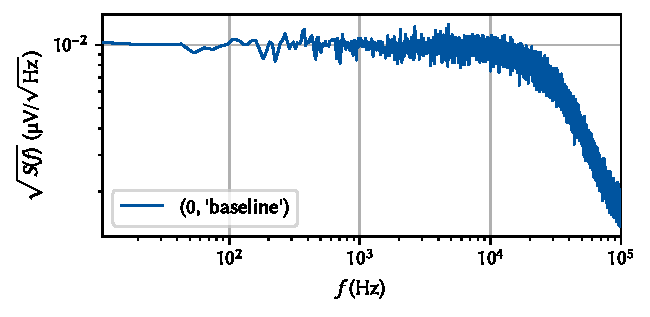
\includegraphics{pdf/spectrometer/workflow_baseline}
    \caption{
        The \pyspeck plot after acquiring the (here: synthetic) baseline spectrum.
        By default, the \gls{asd} = √\gls{psd} is displayed in the main plot.
        Each spectrum is assigned a unique identifier key consisting of an incrementing integer and the user comment, and can be refered to by either (or both) when interacting with the object.
    }
    \label{fig:speck:software:workflow:baseline}
\end{figure}

After acquiring the baseline, he next ungrounds the \gls{daq} to obtain a representative spectrum of the noise in an actual measurement.
He then proceeds by tweaking things on his setup, testing out different parameters, \etc
Every time he changes something, he acquires another spectrum using \code{take()}, labeling each with a meaningful comment for identification.
\begin{listing}[H]
    \begin{py}
        settings = {'f_min': 1e1, 'f_max': 1e5, 'daq': 'connected'}
        spect.take('connected', **settings)
        spect.take('lifted cable', cable='lifted', **settings)
        spect.take('jumped', **settings)
    \end{py}
    \caption[]{
        Code to acquire additional spectra.
        Arbitrary key-value pairs can be passed to the \code{take()} method, which are stored as metadata if they do not apply to any functions downstream in the data processing chain.
    }
    \label{lst:speck:workflow:spectra}
\end{listing}
\begin{figure}
    \centering
    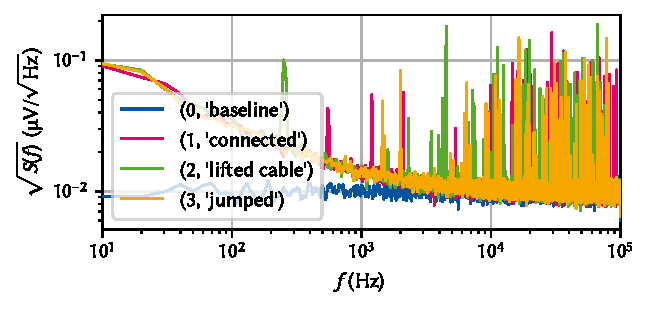
\includegraphics{pdf/spectrometer/workflow_spectra}
    \caption{
        The \pyspeck plot after acquiring additional (synthetic) spectra.
        Each spectrum is uniquely identified by a two-tuple of \code{(index, comment)}.
    }
    \label{fig:speck:software:workflow:spectra}
\end{figure}
The code shown in \cref{lst:speck:workflow:spectra} would then leave him with the spectrometer plot as shown in \cref{fig:speck:software:workflow:spectra}.
While working, Bob realizes he'd like see the signal in the time-domain as well.
He easily achieves this by setting \code{spect.plot_timetrace = True}, which adds an oscilloscope subplot to spectrometer figure as shown in \cref{fig:speck:software:workflow:timetrace}.

\begin{figure}
    \centering
    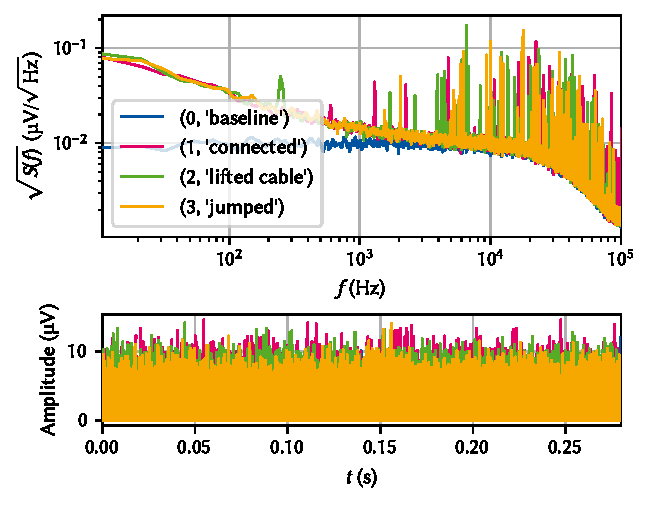
\includegraphics{pdf/spectrometer/workflow_timetrace}
    \caption{
        The \pyspeck plot shown in \cref{fig:speck:software:workflow:spectra} when setting \code{spect.plot_timetrace = True}.
        This adds a subplot that shows the time series data from which the \gls{psd} was computed akin to what an oscilloscope would show.
        Note that this is the entire time series, \ie, the data of length $L$, which is (by default, using Welch's method) segmented for spectrum estimation.
    }
    \label{fig:speck:software:workflow:timetrace}
\end{figure}

Bob now observes that the noise spectra he has recorded display many sharp peaks in particular at high frequencies while the \oneoverf noise floor seems pretty consistent across different measurements.
This makes it harder for him to evaluate whether any of his changes are actually an improvement or not.
The \pyspeck package allows addressing this by plotting the integrated spectra in another subplot.
Bob's spectrometer figure after setting \code{spect.plot_cumulative = True} is shown in \cref{fig:speck:software:workflow:cumulative}.
In the case that \code{spect.plot_amplitude == True}, this new subplot shows the \gls{rms} in the band $[\fmin, f]$,
\begin{align}\label{eq:speck:software:cumulative}
    \rms_S(f)\equiv\rms_S(\fmin, f),
\end{align}
and the band power (\cref{eq:speck:psd:bandpower}) otherwise.

\begin{figure}
    \centering
    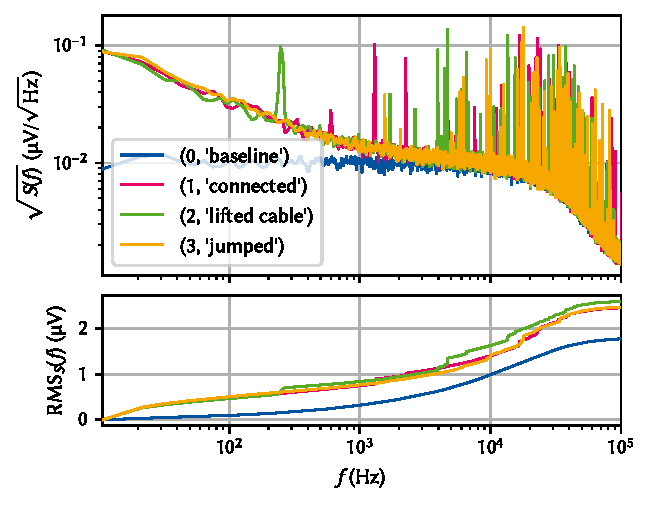
\includegraphics{pdf/spectrometer/workflow_cumulative}
    \caption{
        The \pyspeck plot shown in \cref{fig:speck:software:workflow:spectra} when setting \code{spect.plot_cumulative = True}.
        This adds a subplot that shows the \gls{rms} (see \cref{eq:speck:psd:bandpower}) which can be helpful in evaluating the contribution of individual peaks in the spectrum to the total noise power.
        Both the oscilloscope subplot (\cref{fig:speck:software:workflow:timetrace}) and the \gls{rms} subplot can also be shown at the same time.
    }
    \label{fig:speck:software:workflow:cumulative}
\end{figure}

The cumulative \gls{rms} plot already helps, but Bob would like a more quantitative comparison of relative spectral powers.
Therefore, he rescales the spectra in terms of their relative powers expressed in \unit{\decibel}\sidenote{
    Recall that the decibel is defined by the ratio $L_P$ of two powers $P_1, P_2$ as~\cite{Pozar2012}
    \begin{align*}
        L_P = 10\log_{10}\left(\frac{P_1}{P_2}\right)\,\unit{\decibel}.
    \end{align*}
}
by applying the following settings, which produces the plot shown in \cref{fig:speck:software:workflow:db}:
\begin{py}
    spect.plot_dB_scale = True
    spect.plot_amplitude = False
    spect.plot_density = False
\end{py}
\begin{figure}
    \centering
    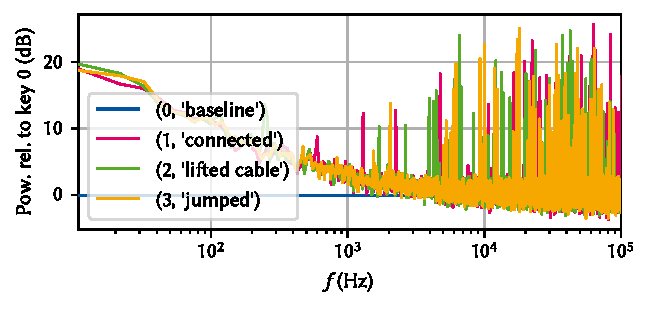
\includegraphics{pdf/spectrometer/workflow_db}
    \caption[The \pyspeck plot in relative mode.]{
        The \pyspeck plot in relative mode.
        Starting from the state in \cref{fig:speck:software:workflow:spectra}, we set \code{spect.plot_dB_scale = True} as well as \code{spect.plot_amplitude = False} and \code{spect.plot_density = False} to compare the relative noise powers with respect to the baseline.
    }
    \label{fig:speck:software:workflow:db}
\end{figure}
The attribute \code{plot_density} controls whether the \emph{\acrlong{psd}} or the \emph{power spectrum} is plotted.\sidenote{
    \label{sidenote:speck:software_vocabulary}
    At this point, we \emph{do} need to distinguish between the \gls{psd} and the power spectrum counter to \cref{sidenote:speck:theory_vocabulary} in \cref{ch:speck:theory}.
    The \gls{psd} and power spectrum are related by the \gls{enbw},
    \begin{align*}
        \text{Spectral density} \xrightarrow{\times\enbw} \text{Spectrum},
    \end{align*}
    which is itself a function of the sampling rate and the properties of the spectral window~\cite{Harris1978},
    \begin{align}\label{eq:speck:software:enbw}
        \enbw = \fs\frac{\sum_n\hat{w}_n^2}{\left[\sum_n\hat{w}_n\right]^2}.
    \end{align}
}
Scaling the data to the power spectrum instead of the density, Bob can get an estimate of the \gls{rms} at a single frequency by reading off the peak height.
Additionally displaying the data in \unit{\decibel} then gives insight into relative noise powers of different spectra.

Bob carries on with his enterprise and continues to acquire spectra until, finally, he finds the source of his noise!
Alas, his spectrometer plot is now overflowing with plotted data when really he just wants to compare the baseline, the original, noisy state, and the final, clean spectrum.
He simply calls
\begin{py}
    spect.hide(*range(2, 10))
\end{py}
to hide the eight spectra of unsuccessful debugging, leaving him with a plot as shown in \cref{fig:speck:software:workflow:success}.

\begin{figure}
    \centering
    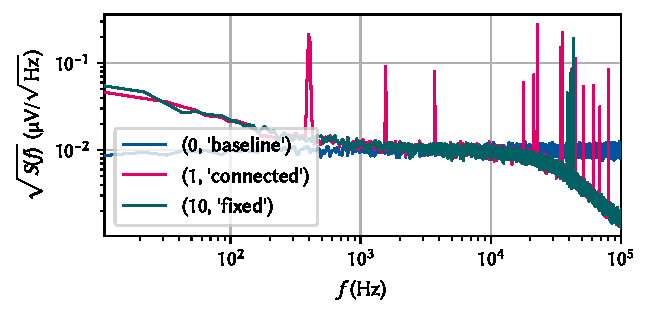
\includegraphics{pdf/spectrometer/workflow_success}
    \caption{
        The \pyspeck plot after multiple additional spectra were acquired and hidden.
        Hiding spectra that one is not interested in anymore is achieved through \code{spect.hide(*range(2, 10))}.
        This is reversed by \code{spect.show(*range(2, 10))}.
        Data can also be dropped (\code{spect.drop(key)}) or deleted (\code{spect.delete(key)}) from the internal cache and disk, respectively.
    }
    \label{fig:speck:software:workflow:success}
\end{figure}

Finally, happy with the results, Bob serializes the state of the spectrometer to disk, allowing him to pick up where he left off at a later point in time:
\begin{py}
    spect.serialize_to_disk('2032-12-24_noise_hunting')
\end{py}
The next week, Bob is asked by his team about his progress on debugging the noise in their setup.
Even though he is working from home that day and does not have access to the lab computer, Bob simply uses his laptop computer and pulls up the \code{Spectrometer} session stored on the server, allowing them to interactively discuss the spectra:
% Important: Spectrometer(
%    bla
%)
% breaks something!
\begin{py}
    file = '2032-12-24_noise_hunting'
    # Read-only instance because no DAQ attached
    spect = Spectrometer.recall_from_disk(savepath / file)
\end{py}
This opens up the plot shown in \cref{fig:speck:software:workflow:success} again.
While they cannot acquire new spectra in this state,\sidenote{
    They could of course always attach a \code{DAQ} instance to the spectrometer and continue as they were.
}
they can still use all the plotting features like showing or hiding spectra, or changing plot types as discussed above.

\subsection{Live spectrum acquisition}\label{subsec:speck:software:features:live_view}
Manually recording spectra in the workflow outlined in \cref{subsec:speck:software:features:serial} becomes tedious at some point, and experimenters tend to become negligent with keeping metadata and comments up to date as they continue to change settings.
Once a certain number of spectra has been obtained, the spectrometer plot also becomes crowded, and hiding old spectra manually is cumbersome.
Moreover, each time a spectrum is captured, data is saved to disk, potentially accruing large amounts of disk space.
For these reasons, the \pyspeck package also offers a non-persistent live mode for displaying spectra continuously.

This mode is facilitated by the \code{qutil.plotting.live_view} module that provides asynchronous plotting functionality based on \matplotlib.
The \code{live_view} module supports both the multithreading and multiprocessing paradigms for concurrency in order to keep the interpreter responsive.
In the former case, the window hosting the figure runs in the main thread and is kept responsive using \matplotlib's GUI event loop mechanisms.
In the latter, the plotting takes place in a separate process, resulting in true parallelism.

The live mode is started with the \code{Spectrometer.live_view()} method.
Data is continuously acquired\sidenote{
    Technically, a very large \code{n_avg} is used.
}
in a background thread using the same \code{DAQ} interface as the serial mode.
Instead of saving the data on disk and managing plotting from \pyspeck, however, the data is fed into a queue.\sidenote{
    A queue is a concurrency mechanism for exchanging data between multiple threads or processes.
}
A \code{live_view.IncrementalLiveView2D} object then retrieves the data from the queue and handles plotting in a GUI event loop.
To start a spectroscopy session with the same parameters as in \cref{subsec:speck:software:features:serial} with a given \code{Spectrometer} object (see \cref{lst:speck:workflow:serial}), we would call
\begin{py}
    view = spect.live_view(f_min=1e1, f_max=1e5, in_process=True)
\end{py}
which would open a figure window such as that shown in \cref{fig:speck:software:live_view}.
Similar to \code{take()}, the data acquisition parameters are passed to \code{live_view()} as keyword arguments.\sidenote{
    The difference is, of course, that we do not need to specify a comment since no data is retained.
}
The \code{in_process} argument specifies if multiprocessing (\code{True}) or multithreading (\code{False}) is used.
Dictionaries with customization parameters for the \code{live_view} object can further be passed to the method.

\begin{figure}
    \centering
    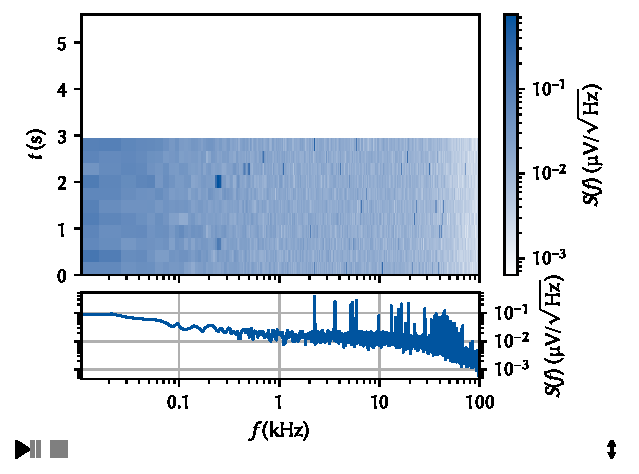
\includegraphics{pdf/spectrometer/live_view}
    \caption[Spectrometer live view]{
        Spectrometer live view.
        The bottom plot shows the most recently acquired spectrum, while the top plot shows a waterfall plot of the most recent ones.
        Data acquisition runs in a background thread, keeping the interpreter responsive and available to interact with instruments, for example.
        The icons in the bottom left and right corner allow interacting with the live view.
    }
    \label{fig:speck:software:live_view}
\end{figure}

% mainfile: ../../main.tex
\chapter{Conclusion and outlook}\label{ch:speck:conclusion}
\AutoLettrine{In} \thispart, I introduced the \pyspeck \python package for interactive, backend-agnostic noise spectroscopy.
I first presented the theory behind spectral noise estimation based on time series analysis in \cref{ch:speck:theory}.
There, I showed how, by the Wiener-Khinchin theorem, the \gls{psd} $S(\omega)$ is related to a time-dependent signal by the Fourier transform of its autocorrelation function $C(\tau)$.
After discretizing the problem, I discussed how the arising spectral windowing introduces distortions in the estimated \gls{psd} through effects such as spectral leakage and scalloping loss.
The introduction of windowing naturally led to the need for a more efficient method of spectrum estimation to avoid data wastefulness.
This is addressed by Welch's method, which trades spectral resolution for estimation accuracy for a given input size by dividing the input into segments and letting them overlap.
Finally, I discussed the various parameters that influence the properties of the spectrum estimate produced by Welch's method.

In \cref{ch:speck:software}, I then introduced the \pyspeck package that facilitates noise spectroscopy based on the theory developed in the previous chapter.
While in principle agnostic to the specific technique (simple periodogram, Bartlett's method, \etc), it employs Welch's method by default to perform efficient estimation of noise \acrlongpl{psd}.
To make noise spectroscopy as approachable as possible, the package provides a unified interface to various hardware and software backends to manage \acrlong{daq}.
Furthermore, it incorporates rich plotting features to ease data analysis and thereby expedite the feedback loop with the lab.
I first outlined the design choices underlying the source code and explained the mechanism employed to infer \gls{daq} settings from, for example, the physical parameters of the resulting spectrum estimate.
I described the interface to drivers for different hardware instruments that makes it possible to use the same user code for spectrum acquisition independent of the specific instrument used for \acrlong{daq} while at the same time keeping the amount of required driver code at a minimum.
Finally, I showcased the interactive features by means of a typical workflow.
Here, the serial approach of recording single spectra that are saved to disk at a time stands in contrast to the non-persistent live mode, where data is continuously acquired and displayed in a separate thread or process.

%\paragraph{Outlook.\label{par:speck:outlook}}
There are several possible avenues for future development of the \pyspeck package.
An obvious case is adding support for more \gls{daq} hardware instruments by implementing \code{DAQ} interfaces.
Modular devices such as those offered by \sidehref{https://www.qblox.com/research}{QBLOX} and \sidehref{https://www.quantum-machines.co/}{Quantum Machines} are on track to become the new standard in quantum technology labs.
Implementing drivers for these instruments would benefit the adoption of both the instruments and the \pyspeck package.
Another valuable addition would be to add support for generic instruments abstracted by \qumada~\cite{Huckemann2025a}.
\qumada is a \qcodes-based measurement framework that provides a unified interface to instruments in order to -- in a similar spirit to \pyspeck's \code{DAQ} interface -- abstract away internals of individual instruments and provide users with a standardized way to interact with them.
This approach should naturally lend itself to a single implementation of the \code{DAQ} class supporting various instruments through the unified \qumada interface.

Next, incorporating noise spectroscopy into the standard measurement workflow of quantum device experiments would allow experimentalists to quickly gauge noise levels as they are performing measurements.
If for some reason the noise changed\sidenote{
    As it happens often, unfortunately.
}
the experimentalist could quickly obtain insight into the noise by analyzing the spectrum.
In a client-server architecture, which is inherently asynchronous, such as Zurich Instrument's \sidehref{https://www.zhinst.com/ch/en/instruments/labone/labone-instrument-control-software}{LabOne} software, this is already possible using the web interface.
But of course the strength of the \pyspeck package stems from its capacity to be utilized in conjunction with any hardware instrument.

\begin{marginlisting}
    \begin{py}[
        fontsize=\footnotesize,%
        breaklines,%
        breakafter=.,%
    ]
        # daq/tee.py
        import dataclasses
        import threading
        import multiprocessing as mp

        from .base import DAQ

        @dataclasses.dataclass
        class TeeDAQ(DAQ):
            settings: mp.managers.DictProxy
            queue: mp.JoinableQueue
            event: threading.Event

            def setup(self, **_):
                settings = self.DAQSettings(self.settings)
                return settings.to_consistent_dict()

            def acquire(self, **_):
                while not self.event.is_set():
                    yield self.queue.get(block=True)
    \end{py}
    \caption[\code{TeeDAQ} template]{
        Template design for a proxy \code{DAQ} implementation to stream noise spectra from an external measurement framework.
        The \code{settings} attribute is a dictionary proxy shared between processes and used to pass acquisition parameters from the measurement framework to \pyspeck.
    }
    \label{lst:speck:conclusion:tee}
\end{marginlisting}

One way to implement such functionality would be to introduce a proxy \code{DAQ} subclass to be used together with the live mode presented in \cref{subsec:speck:software:features:live_view}.
This proxy class would serve as an interface to external measurement software and expose two attributes; first, a data queue, into which the external code could place arbitrary time series data that was obtained during some measurement, and second, a shared dictionary to hold acquisition parameters as these might change between measurements.
Because the live view mode runs in the background, the external measurement framework could push data to the queue whenever new data was taken without obstructing the measurement workflow.

\Cref{lst:speck:conclusion:tee} shows a template design for such a \code{TeeDAQ} class.
The \code{setup()} method ignores the input parameters and instead obtains the current settings from the shared \code{settings} proxy.
Similarly, instead of fetching data from an instrument itself, the \code{acquire()} method attempts to fetch data from the shared \code{queue} and blocks the thread if no data is present, thereby efficiently idling and consuming no resources unless triggered by the external caller.
A measurement framework would then interact with the \code{TeeDAQ} object as exemplarized by the following code:
\begin{py}
    daq = TeeDAQ(...)
    spect = Spectrometer(daq)
    view = spect.live_view()
    ...
    data = measure(fs, n_pts)
    daq.settings.update(fs=fs, n_pts=n_pts)
    daq.queue.put(data)
\end{py}
Measurement frameworks integrating with this interface could thus provide experimentalists live feedback on current noise levels with negligible overhead and minimal code adaptation.

Finally, it might be useful to not only allow estimating \glspl{psd} but also \glspl{csd} or \emph{cross-spectra}.
The cross-spectrum\sidenote{
    Again, we use the two terms interchangably unless otherwise indicated, see \cref{sidenote:speck:theory_vocabulary} in \cref{ch:speck:theory}.
}
is the Fourier transform of not the autocorrelation but the cross-correlation function $C(\tau)$ (\cref{eq:speck:autocorrelation}) between two random processes.
Take a set of processes $\{x_1(t), \allowbreak x_2(t), \allowbreak \dotsc, \allowbreak x_n(t)\}$ that correspond to noise measured at different locations in a sample.
The cross-correlation function between variables $x_i$ and $x_j$ is then given by\sidenote{
    Again assuming wide-sense stationary processes.
}
\begin{align}\label{eq:speck:conclusion:crosscorrelation}
    C_{ij}(\tau) = \expval{x_i(t)\conjugate x_j(t + \tau)}.
\end{align}
This function (and its Fourier pair the cross-spectrum $S_{ij}(\omega)$) quantifies the degree of correlation between noise at site $i$ and noise at site $j$.
Unlike the \emph{auto}-spectrum (or self-spectrum), the cross-spectrum is always a complex quantity, even for real $x_i(t)$.
It is not hard to see that for quantum processors, for example, these kinds of correlations could have significant impact on operation, and on error correction in particular~\cite{Aharonov2006,Nickerson2019,Clader2021}.
To incorporate cross-spectra in the \pyspeck package, only small changes should be necessary.

First, the data acquisition logic would need to be adapted.
Two possible routes suggest themselves here; first, specialized \code{DAQ} classes could be implemented that, in place of yielding one batch of time series data, yield two batches each time they are queried.
This approach first of all requires instruments with multiple channels,\sidenote{
    If one sticks to single \code{DAQ} instances managing single instruments.
}
which is not necessarily given.
Furthermore, it would incur additional coding efforts by having to re-implement each \code{DAQ} class for cross-spectra.
On the other hand, it would arguably make synchronization between channels easier to achieve.

A less involved path would adapt the \code{Spectrometer} class to work with multiple \code{DAQ}s.
This would not involve additional driver work\sidenote{
    Except possibly ensuring thread safety and timing synchronization if multiple \code{DAQ} objects communicate with the same physical instrument.
}
and allow the \code{Spectrometer} object to ensure synchronization between the different \code{DAQ}s.
The internal workflow shown in \cref{lst:speck:daq:workflow} would then need to be slightly adapted to the code shown in \cref{lst:speck:conclusion:cross_workflow}.
The downside of this approach is that synchronization of different instruments or channels would need to be taken care of externally.

\begin{listing}[htpb]
    \begin{py}
        daq_1 = MyDAQ(driver_handle, channel=1)
        # Or MyOtherDAQ(driver_handle_2) if another instrument
        daq_2 = MyDAQ(driver_handle, channel=2)
        daqs = (daq_1, daq_2)

        parsed_settings = [daq.setup(**user_settings) for daq in daqs]
        assert all_equal(parsed_settings), "DAQ settings do not match"

        acquisition_generators = [daq.acquire(**parsed_settings[0])
                                  for daq in daqs]
        for data_buffers in zip(*acquisition_generators):
            estimate_csd(*data_buffers)
    \end{py}
    \caption[Proposed \code{DAQ} workflow for cross-spectra]{
        Proposed \code{DAQ} workflow for estimating cross-spectra.
        Each hardware channel (same or different instruments) is assigned to a \code{DAQ} object.
        After instrument configuration, it is asserted that the parameters match.
        Finally, data is fetched from both channels and fed into a \gls{csd} estimator.
        Note that triggering would need to be implemented externally.
    }
    \label{lst:speck:conclusion:cross_workflow}
\end{listing}

Further code adaptations would involve minor changes such as replacing the spectrum estimator with \code{scipy.signal.csd()}~\sidecite{CSDScipy} for \gls{csd} estimation\sidenote{
    In practice, working with the normalized \gls{csd}, or correlation coefficient~\cite{Rojas-Arias2023,Yoneda2023}
    \begin{align}
        r_{ij}(\omega) = \frac{S_{ij}(\omega)}{\sqrt{S_{ii}(\omega)S_{jj}(\omega)}}
    \end{align}
    with $S_{ii}(\omega)$ the \gls{psd} of process $x_i$ would likely be more favorable.
}
and make the plotting conform to complex data.\sidenote{
    It could be worthwile to add a subplot to display both the magnitude and phase of the complex quantity $S_{ij}(\omega)$.
}
% TODO:
%  - improve this part?
%  - spectrogram?
%  - rms plot in live view?


\pagelayout{wide} % No margins
\part{Characterization and Improvements of a Millikelvin Confocal Microscope}
\label{part:setup}
\pagelayout{margin} % Restore margins
\glsresetall

% mainfile: ../../main.tex
\chapter{Introduction}\label{ch:setup:introduction}

\begin{partcontribs}
    Parts of the results presented in \thispart have been published in Reference~\sidecite{Descamps2024}.
    Thomas Descamps\sidenote[a]{Then at \RWTHFZJ} and Feng Liu\sidenotemark[a] originally designed the setup together with Hendrik Bluhm\sidenote[b]{\RWTHFZJ} and constructed it.
    Julian Ritzmann\sidenote[c]{\RUB} and Arne Ludwig\sidenotemark[c] grew the wafer on which Matthias Künne fabricated the sample used to measure the electron temperature in \cref{sec:setup:cooling:etemp}.
    The chip used to measure photon antibunching in \cref{sec:setup:optics:g2} was grown by Xuelin Jin.\sidenote[d]{\FZJ}
    Marcus Eßer\sidenote[e]{\RWTH} kindly lent the accelerometer used in \cref{sec:setup:vibrations:accel}.
\end{partcontribs}

\lettrine[lines=3,lhang=0.33,loversize=0.25,depth=1]{Q}{uantum} technology is maturing and entering the realm of commercial application~\cite{Schleich2016,Mohseni2017,QTBMBF,QTCEN,QTEU}.
Despite this progress, its potential is arguably far from fully tapped.
From the perspective of the physicist, quantum technology can not only serve the industrial sector, though, but also become a new tool in the researcher's belt to explore new physics on the nanoscale, where quantum mechanics governs the behavior of individual particles as well as many-body interactions and collective effects.
Given the multidisciplinarity of the field, this presents a unique opportunity to explore in particular the intersection of different areas of physics such as optomechanics~\cite{Aspelmeyer2014,Barzanjeh2022}, quantum thermodynamics~\cite{Goold2016,Deffner2019,Cangemi2024} and batteries~\cite{Campaioli2024}, quantum gravity~\cite{Degen2017,Bass2024}, and more.

In the solid state, electrical and optical properties dominate.
Here, their intersection brings together two of the perhaps technologically most advanced and permeating branches of physics.
The small energy scales involved in electronic \emph{intra}-band effects or many-body correlations often necessitate extremely low temperatures in the Millikelvin range for observation.
While optical effects on the other hand are fairly robust due to their large energy scales in the visible range,\sidenote{
    Typically quoted as \qtyrange{380}{750}{\nano\meter} corresponding to \qtyrange{1.65}{3.26}{\electronvolt}.
}
semiconductors or semimetals such as graphene allow optical \emph{inter}-band transitions and as such coupling between the valence and conduction band, which in themselves are predominantly governed by low-energy physics.
Thus, observing many-body effects of quasiparticle excitations such as a \gls{bec} of excitons~\cite{Kohn1970,High2012,Combescot2017,Morita2022,Zhang2024}, for example, places high demands on the experimental setup, requiring not only very low temperatures but also optical access.

For quantum technologies, the development of a quantum network based on optically interfaced solid-state spins is among the foremost goals~\cite{Awschalom2018,Azuma2023,Heindel2023,Zajac2025}.
There, single optical photons are used to transmit quantum information across long distances and qubits encoded in single spins -- electronic or nuclear -- are used to store and process information locally.
Owing to their small magnetic moment and strong Coulomb interaction, electron spin qubits usually require temperatures well below \qty{1}{\kelvin} for high-fidelity operation, and a coherent interface between these and a \enquote{flying qubit} -- a photon encoding information, for example, in its helicity or time-of-arrival degree of freedom -- would thus also need to be placed in an optically accessible cryostat capable of reaching such low temperatures.

\Citeauthor{Descamps2024}~\cite{Descamps2021,Descamps2024} presented a free-space confocal microscope integrated into a fully wired cryogen-free \gls{dr} (\odin) that facilitates such experiments.
In the following, I give a brief outline of the setup described in more detail in \citer{Descamps2021}.
The microscope is constructed with the optics fixed in place on top of the cryostat, alleviating the need to remove and re-align them when opening and closing the cryostat.
Optical fibers deliver light to the cryostat from the optical table and back, simplifying the connection between the two components.
On the optical table, a tunable \gls{cw} \ch{Ti}:sapphire laser\sidenote{
    A spectrally filtered, pulsed \unit{\femto\second}-laser (\pulsedlaser) is also available but unused in \thethesis.
}
(\tisalaser) generates coherent radiation that is attenuated by a variable \gls{nd} filter mounted on an electrically controlled rotation stage (\thorlabsrotator) and can be blocked by an electrically controlled filter flipper (\thorlabsflipper).
The attenuated light is coupled into a \gls{smf} patch cable (\thefiber) and delivered to the optical head on top of the cryostat, which I describe and analyze in more detail in \cref{ch:setup:optics}.
Waveplates mounted on piezoelectric rotation stages (\rotator) with controller \rotatorcontroller allow electromechanical control of the polarization state.
The sample is mounted on three piezoelectric linear steppers (\positioner) with controller \positionercontroller that allow for precise control of the sample position.
Light collected from the sample is coupled into another \gls{smf} patch cable on the optical head and, on the optical table, launched into a diffraction grating spectrometer (\thespectrometer) with a focal length of \qty{1}{\meter} \acrshort{na}-matched to the fiber by a pair of singlet lenses.
The spectrometer houses two gratings (\qty{600}{gr\per\milli\meter} and \qty{1800}{gr\per\milli\meter}) mounted on a rotating turret.
Two exit ports selectable by an electrically controlled mirror let the dispersed light exit the spectrometer onto either a thermoelectrically cooled \gls{ccd} (\theccd) or, through an adjustable slit allowing spectral filtering, into a \gls{hbt} interferometer.
The interferometer consists of a 50:50 \gls{bs} on whose exit ports the light is focused into two \glspl{mmf} connected to an \gls{apd}-based \gls{spcm} (\thespcm) each.
A streaming time-to-digital converter (\tagger) then assigns time tags to the output pulses of the \glspl{spcm} heralding the arrival of a single photon.

The entire setup thus consists of various different components of different nature -- mechanical, optical, electrical, or a combination thereof -- made by various different manufacturers, making the unified control of all instruments challenging.
During the work on \thethesis, I extended the \python driver coverage within the \qcodes framework to include all components that provide an \gls{api} for external control.
This enables fully remote operation and allows for complete automation of the setup.\sidenote{
    Remote turn-on of the laser still requires explicit user input for safety reasons.
}
I furthermore implemented the bottom-loading technique for fast sample exchange, whereby the \gls{mxc} is held at \qty{10}{\kelvin} while the sample puck is removed or replaced using a special adapter from below.
Turnaround cycles of approximately one day from base temperature to base temperature can be achieved in this way, in contrast to a full warm-up and cooldown cycle time including removal and replacement of all cryostat shields of one week.
The optical alignment turns out to be remarkably stable during this procedure and it is usually not required to manually adjust it after a bottom loading cycle.

In \thispart, I analyze, characterize, and improve upon three different parts of this measurement setup.
First, I investigate the refrigeration capabilities of the \gls{dr} to address the question of how the modifications for optical access impact the cooling performance (\cref{ch:setup:cooling}).
There, I present measurements of various sources of heating and compare them to the available cooling power before turning attention to the achievable electron temperature in a \GaAsAlGaAs quantum dot.
In \cref{ch:setup:optics}, I then discuss the confocal microscope itself, that is, the optics mounted to the cryostat, including the objective and ocular lenses as well as the coupling to the \glspl{smf}.
I review the fundamentals of the relevant physics in order to guide the reader through the lens selection process and subsequently compare the estimated setup efficiency to measurements, focusing on the mode profile of dipole radiation emitted from a point source inside a dielectric slab.
Moreover, I characterize the laser spot on the sample using the imaging capabilities of the optical head as well as the cross-polarization extinction performance.
To validate the optical performance of the microscope, I demonstrate that signatures of non-classical light, specifically photon anti-bunching from a \gls{saqd} single-photon source, can be readily observed.
Lastly, in \cref{ch:setup:vibrations}, I address the impact of vibrations introduced by the cryostat's operation on the microscope performance.
Given that we would like to resolve features on the micrometer scale, and need to couple light emitted from the sample into a \gls{smf} with \gls{mfd} of \qty{5}{\micro\meter}, random displacements induced by the acoustic waves generated by the cryostat's \gls{ptr} during operation can potentially limit the microscope's capabilities severely.
I take a passive air spring suspension approach to decouple the cryostat from a static rigid reference frame and allow it to be displaced freely and in-phase with the external perturbation.
Employing two different techniques, I characterize the vibration noise using the tools developed in \cref{part:speck} and show that the vibrations can indeed be attenuated to a degree sufficient for operation of the microscope.

% mainfile: ../../main.tex
\chapter{Cryostat performance}\label{ch:setup:cooling}
\AutoLettrine{An} essential feature of the confocal microscope discussed in \thethesis is its capability to perform optical measurements at Millikelvin temperatures.
As individual quantum systems are singled out for applications in quantum technology, thermal excitations with energy $\kb T = \qty{86}{\micro\eV\per\kelvin}\times T$ quickly become the dominating energy scale and overshadow the desired effects.
Hence, typical energies in the solid state on the \unit{\micro\eV} scale, such as Zeeman energies of individual spins with energy $\mub B = \qty{58}{\micro\eV\per\tesla}\times B$, require temperatures well below \qty{1}{\kelvin} to suppress thermal excitations and maintain $\kb T \ll \mub B$.

By design the \odin dry \gls{dr} housing the microscope is rated for base temperatures at the \acrfull{mxc} plate below $\Tmxc=\qty{10}{\milli\kelvin}$ and a cooling power of \qty{450}{\micro\watt} at $\Tmxc=\qty{100}{\milli\kelvin}$.
However, several factors, both passive and active, introduce additional heat loads that can potentially raise the base temperature if too large:
\begin{enumerate}
    \item \label{itm:setup:cooling:wiring}
    DC and RF wiring.
    These introduce thermal links between the sample and higher temperature stages as well as add noise that raises the electron temperature in the sample.
    \item \label{itm:setup:cooling:positioners}
    Wiring and operation of the \positioner nanopositioners.
    The nanopositioners require special low-impedance connections to ensure a large enough bandwidth for the slip-stick mode of operation.
    Moreover, the resistive position readout introduces additional heating.
    \item \label{itm:setup:cooling:optical}
    Optical access.
    The free-space optical access requires a direct \gls{los} port to the sample.
    This inevitably allows infrared radiation from room temperature into the cryostat, something that is usually painstakingly prevented when designing a cryostat.
    Furthermore, optical experiments involve irradiating the sample with a highly focused laser beam, some of which will be absorbed and contribute to heating.
\end{enumerate}

In this chapter, I characterize the cooling performance of the dry \gls{dr} housing the microscope in various ways.
I first discuss the cooling power in terms of the base temperature \Tmxc reached for different configurations in \cref{sec:setup:cooling:power}.
This is often quoted as the bath, lattice, or \emph{phonon} temperature,\sidenote{
    This terminology can be misleading as the phonon temperature can also be measured with a quantum transport device, which will most likely see a different phonon temperature than the thermometer on the mixing chamber plate because of a temperature gradient between the heating source close to the sample and sink (the mixing chamber) close to the thermometer.
}
and can be read out using the resistive \ch{RuO_2} thermometry setup installed in the \gls{dr}.
Then, in \cref{sec:setup:cooling:etemp}, I present measurements of the \emph{electron} temperature, a quantity that is arguably more expressive of the cryostat's capability to perform precise measurements as it is more sensitive to, for example, electrical noise introduced by the wiring.
In order to avoid duplication, I refer readers to References~\cite[Section 4.1]{Descamps2021} and~\cite[Section II]{Descamps2024} for more details on the cryostat layout and design.

\section{Cooling power}\label{sec:setup:cooling:power}
The base temperature (\Tmxc) can be read out from the resistance bridge connected to the gas handling PC controlling the cryostat.
Two different thermometers are installed on the mixing chamber, a Cernox\textsuperscript{\textregistered} sensor that works in the range from room temperature down to around \qty{2}{\kelvin} for cooldown, and a \ch{RuO_2} sensor that works from \qty{30}{\kelvin} down to the Millikelvin regime for base temperature operation.
The resistance bridge performs a four-terminal measurement of the sensor resistance and converts it to a temperature according to a sensor-specific calibration $\Tmxc(R_{\ch{RuO_2}})$.
Since the particular sensor installed in the system was only calibrated down to \qty{30}{\milli\kelvin}, I had to extrapolate the calibration curve as the system reaches lower temperatures than this, and hence the temperatures below this threshold quoted here are not guaranteed to be correct.

\begin{marginfigure}
    \centering
    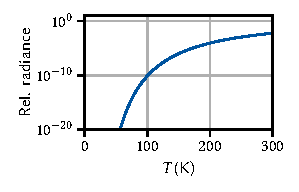
\includegraphics{img/pdf/setup/black_body_radiance}
    \caption[\imgsource{img/py/setup/cooling_power.py}]{
        Relative black-body radiance obtained by integrating \cref{eq:setup:cooling:blackbody} from $\lambda = \qtyrange{0}{4.5}{\micro\meter}$ and normalizing to the total radiance.
        At $T=\qty{300}{\kelvin}$, the fraction of total radiance residing in the high-energy part of the spectrum is still only \qty{0.6}{\percent}.
    }
    \label{fig:setup:cooling:blackbody}
\end{marginfigure}

With the configuration described in \citer{Descamps2021}, the \gls{dr} reached a base temperature of $\Tmxc = \qty{30}{\milli\kelvin}$.
This included all DC and \gls{rf} wiring as well as a single \gls{ar}-coated window sealing the vacuum space on top of the fridge for optical access.
To investigate the influence of ambient thermal radiation entering the cryostat through the optical access port, or, more generally, radiation from the higher- to lower-temperature stages, I measured the base temperature for two additional configurations; once with an additional \gls{ar}-coated window inserted into the optical path on the Cold ($\sim\qty{80}{\milli\kelvin}$) plate, and once with three windows installed on the \gls{pt1} ($\sim\qty{50}{\kelvin}$), \gls{pt2} ($\sim\qty{4}{\kelvin}$), and Still ($\sim\qty{800}{\milli\kelvin}$) plates.
The windows (\thewindow) are made from UV fused silica with \gls{ar} coating.\sidenote{
    Depending on the manufacturer, the coating for the range \qtyrange{650}{1050}{\nano\meter} is called \acrshort{bbar} VIS-\acrshort{nir} or \acrshort{bbar}-B.
}
The manufacturer quotes a typical reflectance of \qty{0.25}{\percent} in the relevant wavelength range of \qtyrange{700}{1000}{\nano\meter}, while the glass is largely transmissive for wavelengths below $\lambda_{\mr{cutoff}}\sim\qty{4.5}{\micro\meter}$.
Since the spectral radiance of thermal black-body radiation~\cite{Planck1900}
\begin{equation}\label{eq:setup:cooling:blackbody}
    B_\lambda(\lambda, T) = \frac{2 h c^2}{\lambda^5}\frac{1}{\exp(\flatfrac{hc}{\lambda\kb T}) - 1}
\end{equation}
is small up to $\lambda_{\mr{cutoff}}$ at low ($\leq\qty{300}{\kelvin}$) temperatures as shown in \cref{fig:setup:cooling:blackbody}, we expect the windows be largely opaque to thermal radiation and hence be quite effective in reducing the radiative heat load.
As further the radiative power scales with $T^4$ and there is at the same time more cooling power available at higher-temperature stages, installing windows there result in an overall better performance.

\begin{margintable}
    \centering
    \footnotesize
    \caption{
        \Gls{mxc} temperature for different configurations of \gls{ar} coated windows (\thewindow) inside the \gls{dr}.
    }
    \label{tab:setup:cooling:windows}
    \begin{tabular}{lr}
        \toprule
        \textsc{Windows}                      & $T_\mathrm{\acrshort{mxc}}$ \textsc{(mK)} \\
        \midrule
        None                                  & 30.0                                      \\
        Cold                                  & 11.0                                      \\
        \acrshort{pt1}, \acrshort{pt2}, Still & 7.9                                       \\
        \bottomrule
    \end{tabular}
\end{margintable}

\Cref{tab:setup:cooling:windows} shows the measured mixing chamber temperatures for the different window configurations.
Indeed, already a single window installed on the Cold plate significantly reduces the base temperature.
While the windows do introduce additional reflections of the laser spot when imaging the sample, their intensity is low enough, and their position on the camera far enough away from the main spot, to be an issue.
On the contrary, the reflections can be quite useful when aligning the laser spots from the two arms of the optical head by aligning them in such a way that the reflections overlap.

Besides the ambient radiation, there is also the heat load introduced by the partial absorption of the laser excitation when conducting optical measurements.
In order to both characterize the heat load and measure the absorptance \absorptance of our sample, I irradiated a flip-chip-bonded membrane sample (see \cref{part:exp}) with the laser at \qty{815}{\nano\meter} and measured the increase in base temperature.
The sample consists of a \qty{220}{\nano\meter} thick \GaAsAlGaAs membrane glued with epoxy to a \ch{Si} host substrate chip for handling.
As the samples are flip-chip bonded, light that is transmitted through the chip without being absorbed or reflected will then hit the surrounding puck and scatter.
Thus, to be precise, I measured $\absorptance+\transmittance$ this way, where \transmittance is the transmittance, assuming that light that exits the membrane will be absorbed \emph{somewhere} and contribute to heating.
I will nonetheless refer to the measured quantity as simply \absorptance.
In \cref{sec:exp:tmm}, I analyze the absorptance, reflectance, and transmittance of such membrane samples in more detail.

With the power meter mounted in the transmission direction of the excitation arm of the optical head (\cf \cref{fig:setup:optics:optical_path}), I measured the amount of power directed towards the sample by scaling the measured power with the ratio of transmittance and reflectance of the \gls{bs}, $\transmittance\div\reflectance\approx\num{15}$.
Assuming negligible losses on the way towards the sample, I then recorded the mixing chamber temperature as function of laser power.
To relate that change in temperature to a heat load $\dot{Q}$ deposited on the sample, I calibrated the cooling power of the \gls{dr} using the built-in heaters.
Setting a heater power and waiting for the mixing chamber temperature to settle yields the cooling power $P_{\mr{cool}}$ as function of temperature \Tmxc, which is expected to follow the quadratic relationship~\cite{DeWaele2011}
\begin{equation}\label{eq:setup:cooling:dr_power}
    P_{\mr{cool}} = \dot{Q} = \alpha \Tmxc^2 + \beta.
\end{equation}
We can then use a simple model of absorption of the laser on the sample in thermal equilibrium,
\begin{equation}\label{eq:setup:cooling:absorptance}
    P_{\mr{cool}} = P_{\mr{nr}} = \absorptance P_{\mr{laser}},
\end{equation}
where $P_{\mr{nr}}$ is the amount of power deposited into nonradiative emission channels causing heating of the lattice, to relate the incident laser power $P_{\mr{laser}}$ to the cooling power and thus obtain the absorptance \absorptance.

\begin{marginfigure}[*-15]
    \centering
    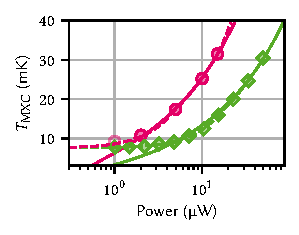
\includegraphics{img/pdf/setup/laser_heating}
    \caption[\imgsource{img/py/setup/cooling_power.py}]{
        \Acrlong{mxc} temperature as function of heater (magenta) and laser (green) power.
        Solid lines are fits to \cref{eq:setup:cooling:dr_power} including only the solid markers.
        Green dashed line is a quadratic smoothing spline fit to all laser data points.
        Magenta dashed line is the laser spline scaled to match the heater data with fitted factor $\absorptance=\qty{28}{\percent}$, corresponding to the fraction of laser power absorbed and non-radiatively emitted.
    }
    \label{fig:setup:cooling:laser}
\end{marginfigure}

\Cref{fig:setup:cooling:laser} shows data sets obtained with the \gls{mxc} heater (magenta) and laser (green).
The solid lines are fits to \cref{eq:setup:cooling:dr_power} including the solid data points only as at low powers there is clearly a deviation from the square-root relationship between the two.
Comparing the fit results for $\alpha$, we obtain $\absorptance = \qty{28.5}{\percent}$.
Alternatively, we can fit a quadratic smoothing spline to the laser data (magenta dashed line) and fit a version scaled according to \cref{eq:setup:cooling:absorptance} to the heater data (green dashed line).
This yields $\absorptance = \qty{28.1}{\percent}$ in good agreement to the value obtained from fitting the theoretical model (\cref{eq:setup:cooling:dr_power}).
Furthermore, the data shows that only at laser powers above \qty{10}{\micro\watt} the \gls{mxc} heats up appreciably.

Lastly, let us address the impact of the \positioner position readout.
The nanopositioners are crucial in the operation of the microscope as they are used to position the sample with respect to the focal spot of the objective lens.
They operate in slip-stick mode which naturally generates heat through friction when moving.\sidenote[][*-12]{
    In physics terms, the slip-stick scheme corresponds to alternating adiabatic and diabatic ramps.
    Slowly ramping up a DC voltage elongates the piezoelectric element by a small amount and moves the positioner table.
    When quickly jumping back down to \qty{0}{\volt}, the table slips and stays in place while the piezo contracts back to its equilibrium elongation.
    This way, distances much larger than the piezoelectric elongation can be travelled.
    Staying in the adiabatic regime results in reproducible displacements but also limits the travel.
}
However, the resistive position readout also contributes to heating, so in order to assess if the readout should be switched off when it is not required to avoid unnecessarily elevated cryostat temperatures, I measured \Tmxc as a function of readout voltage.
Note that the \positionercontroller piezo controller offers the option of lock-in measurement for readout, which should be enabled as it improves the \gls{snr} and thus allows for a smaller readout voltage $V_{\mr{AC}}$.

\begin{marginfigure}[*-8]
    \centering
    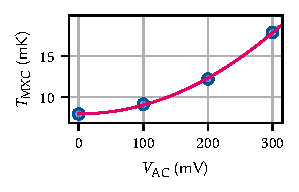
\includegraphics{img/pdf/setup/anc_readout_heating}
    \caption[\imgsource{img/py/setup/cooling_power.py}]{
        \Acrlong{mxc} temperature as function of nanopositioner AC readout voltage.
        The secondary axis indicates the conversion from \Tmxc to power obtained in \cref{fig:setup:cooling:laser} which is approximately linear in this regime, leading to the expected $P\sim R\inverse V_{\mr{AC}}^2$ behavior.
        Solid line is a fit to the power with $R=\qty{16.9}{\kilo\ohm}$.
    }
    \label{fig:setup:cooling:anc}
\end{marginfigure}

\Cref{fig:setup:cooling:anc} shows the temperature as function of $V_{\mr{AC}}$, as well as the equivalent power from the calibration performed in \cref{fig:setup:cooling:laser}.
The expected Ohmic behavior is evident, resulting in a resistance of $R=\qty{16.9}{\kilo\ohm}$.
We can conclude that for $V_{\mr{AC}} < \qty{100}{\milli\volt}$, heating from the positioner readout is negligible.
In this regime, the \gls{snr} of the measurement is acceptable, and hence the readout can be safely left enabled without affecting the heat budget of the cryostat.

\section{Electron temperature}\label{sec:setup:cooling:etemp}
In the previous section, I discussed various sources of heating of the cryostat temperature measured at the mixing chamber plate using a commercial resistive thermometer.
An arguably more relevant metric for quantum device experiments is the electronic temperature which -- depending on how it is measured in detail -- corresponds to the temperature of the Fermi distribution of electrons in or coupled to a reservoir rather than the temperature of the crystal lattice.
Precisely because the behavior of these quantum devices depends so sensitively on the electron temperature, one can also flip this relationship on its head and use them to \emph{measure} the temperature, an instance of single controlled quantum systems being used as highly sensitive probes of physical quantities known as \emph{quantum sensing}~\cite{Degen2017}.
\Glspl{gdqd} hosted in the \gls{2deg} of a semiconductor heterostructure offer several different ways of measuring the electron temperature that are each different in subtle ways.
For example, using an adjacent charge sensor, one can measure the width of a lead\sidenote{
    A \enquote{lead} is a reservoir of charge carriers coupled to a quantum dot.
}
(charge) transition~\cite{Maradan2014} or the width of the inter-dot (charge) transition in a double \gls{qd}~\cite{DiCarlo2004}.
Simpler still, one can measure the width of a Coulomb resonance in the conductance through a \gls{qd}~\cite{Ihn2009,Maradan2014}.
All of these methods rely on some form of energy reference scale that relates the energy of an electron confined in a \gls{qd} to some externally controlled parameter such as a voltage, however.
Typically this is the so-called \emph{lever arm} $\alpha$, which is the constant of proportionality between the plunger gate voltage and the electrochemical potential $\mu_N$ for adding the $N$th electron to the quantum dot~\cite{Ihn2009}.
It can be measured using pulsed-gate spectroscopy~\cite{Fujisawa2001,Harbusch2010}, photon-assisted tunneling~\cite{Kouwenhoven1994}, or finite-bias spectroscopy (Coulomb diamonds)~\cite{Kouwenhoven2001,Ihn2009}, for example.

\begin{marginfigure}
    \centering
    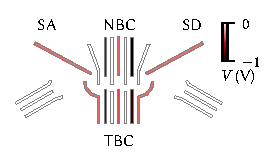
\includegraphics{img/pdf/setup/diamonds_gl}
    \caption[\imgsource{img/py/setup/transport.py}]{
        Gate layout of a quadruple \acrlong{qd} with two charge sensor \glspl{qd} from \citer{Cerfontaine2019}.
        Ohmic contacts used for transport measurements are right (left) of SA (SD).
        NBC and TBC are the gates in the middle of the top and bottom rows.
        The gates are colored according to the voltages applied with the device hosting a single large \gls{qd} in the few-electron, sequential tunneling regime.
    }
    \label{fig:setup:cooling:etemp:gl}
\end{marginfigure}

Here, I chose the simplest of these techniques that require the least tune-up to avoid unnecessarily complicating things.
That is, I formed a single \gls{qd} in a gated \GaAsAlGaAs heterostructure and extracted the lever arm from Coulomb diamonds and the electron temperature from the conductance trace of a Coulomb resonance at zero bias in the sequential tunneling regime.
The gate layout of the device used is shown in \cref{fig:setup:cooling:etemp:gl}.
Designed for two-qubit experiments with two-electron spin qubits by \citet{Cerfontaine2019}, I tuned the device to host a single large \gls{qd} in the center of the device.
The gates are color-coded according to the voltages applied with the device in the few-electron regime.
I applied a bias voltage at the Ohmic contact situated to the right of gate SA\sidenote{
    I use the same naming scheme for gate electrodes as Reference~\cite[Chapter 7]{Cerfontaine2019}.
}
using a home-built \decadac voltage source and measured the current at the Ohmic contact to the left of gate SD using a \baseltia I/V converter with non-inverting input shorted to ground.
Gate voltages were also supplied by the \decadac, divided by six and low-pass filtered at room temperature in the \gls{bob}.
All but the four long gates (RFA--RFD) coming in from the top of the device were connected to the filtered DC lines as described in \citer{Descamps2021}.\sidenote{
    The sample is mounted on a high-frequency \gls{pcb} whose on-board capacitors form the second link in a second-order $RC$ low-pass filter.
    Between the \gls{pcb} and the $z$-axis nanopositioner, there is a \ch{Cu} plate connected directly to the top interface of the sample puck via flexible braids for heat sinking as the positioners have poor thermal conductivity~\cite{Descamps2024}.
    However, this plate is also crucial for providing a ground connection for the \gls{pcb} and, consequently, the functioning of the $RC$ low-pass, as the positioners are also not electrically conductive.
}
The former were connected to RF lines attenuated with \qtylist{20;6;0;3}{\decibel} attenuators mounted to the \gls{pt2}, Still, Cold, and \gls{mxc} plates, respectively, and connected to a \hdawg but unused during these experiments.

To tune the electrochemical potential in the dot, I set up a virtual plunger gate~\cite{Botzem2018} from a linear combination of the gates NBC and TBC by performing a two-dimensional sweep of TBC against NBC\@.
From the slope $m$ of a charge transition in the voltage space spanned by TBC and NBC, I computed the weights of the virtual gate in terms of the physical gates as
\begin{equation}
    V_{\mr{p}} = \frac{1}{\sqrt{1 + m^2}}\left(\mr{TBC} + \abs{m}\times \mr{NBC}\right).
\end{equation}
Following this procedure, even a dot that does not lie in the middle between the two gates, \ie, couples more strongly to one than the other gate, should not move in position when changing the virtual gate voltage.
Having set up the virtual plunger gate, I performed a Coulomb diamond measurement wherein the (virtual) plunger gate is swept as the source-drain bias voltage is varied.\sidenote{
    In this case, the source-drain bias is asymmetric as the drain is always grounded and only the electrochemical potential of the source reservoir is changed.
    This does not qualitatively change the physics of the measurement, though.
}
The left panel of \cref{fig:setup:cooling:etemp:diamonds} shows the current of the Coulomb diamond measurement.
Starting from zero bias, when current can only flow through the Coulomb-blockaded \gls{qd} when both source and drain are aligned with an energy level in the dot, increasing the bias voltage opens up the \emph{bias window}, allowing current to flow as long as the dot's energy level is inside the window.
This defines areas of zero (blockaded) current within the space of plunger and bias voltage that takes on the shape of a diamond whose height (along the bias axis) is given by the energy penalty of adding another electron to the dot~\cite{Ihn2009},
\begin{equation}
    E_\mr{add} = \mu_{N+1} - \mu_N = E_c + \Delta E,
\end{equation}
where $\mu_N$ is the electrochemical potential of the dot with $N$ electrons, $E_c$ is the charging energy due to Coulomb repulsion, and $\Delta E$ is the single-particle energy spacing.
At the same time, the width of a diamond (along the gate voltage axis) is given by
\begin{equation}
    \Delta V_{\mr{p}} = \alpha\inverse E_\mr{add},
\end{equation}
implying that we can extract the lever arm $\alpha$ from the geometry of the diamonds.
Drawing lines with slopes $m_1$ and $m_2$ along the onsets and offsets of current through the Coulomb resonance at zero bias (dashed gray lines), I obtained
\begin{equation}
    \alpha = \abs{\Delta m} = \abs{m_1 - m_2} \approx\qty{0.11}{\eV\per\volt}.
\end{equation}

\begin{figure*}
    \centering
    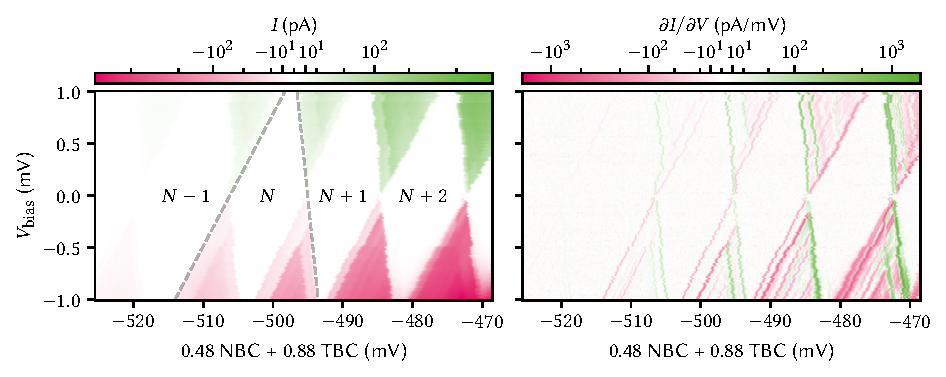
\includegraphics{img/pdf/setup/diamonds}
    \caption[\imgsource{img/py/setup/transport.py}]{
        Coulomb diamond measurement of the single \gls{gdqd} confined by applying static voltages to the gates shown in \cref{fig:setup:cooling:etemp:gl}.
        The left panel shows the current measured with a \gls{tia} with a bias applied on one side of the device.
        The horizontal axis shows the virtual plunger gate swept for each bias voltage indicated on the vertical axis.
        The difference in slope of the dashed gray lines around the $N$-electron diamond yields the lever arm $\alpha$ converting virtual plunger gate voltage to (relative) energy inside the dot.
        From the fact that the slopes are not equal up to a sign we can infer that the coupling to source and drain reservoirs is unequal also, indicating that either the dot is situated closer to SA than to SD, or the topology of the tunneling contacts in the \gls{2deg} is different due to different electrostatic potential.
        The right panel shows the differential conductance obtained from differentiating the data from the left panel along the plunger gate axis.
        Clearly visible are several additional transition lines which correspond to excited states inside the dot becoming energetically available within the bias window.
    }
    \label{fig:setup:cooling:etemp:diamonds}
\end{figure*}

Although not of particular interest for the electron temperature, a Coulomb diamond measurement can also be used for excited state spectroscopy.
Computing the differential conductance $\partial I/\partial V_{\mr{p}}$ makes visible a host of additional transition lines in the conducting region of the map (right panel of \cref{fig:setup:cooling:etemp:diamonds}).\sidenote[][*-2]{
    Features inside the blockaded region can also occur, indicative of co-tunneling.
}
These correspond to excited states of the quantum dot entering the bias window.
Their sign depends on the tunnel coupling of the state to source and drain~\cite{Ihn2009}.

\begin{marginfigure}[*-3]
    \centering
    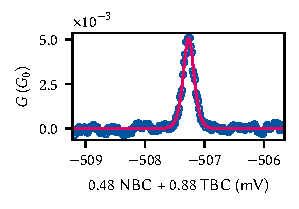
\includegraphics{img/pdf/setup/coulomb_resonance}
    \caption[\imgsource{img/py/setup/transport.py}]{
        Conductance of a Coulomb resonance in the sequential tunneling regime.
        The magenta line is a fit to \cref{eq:setup:cooling:etemp:resonance} with $T = \qty{74.9}{\milli\kelvin}$ and $\Gamma = \qty{0.524+-0.005}{\micro\eV}$.
    }
    \label{fig:setup:cooling:etemp:resonance}
\end{marginfigure}

Having measured the energy reference scale, the lever arm $\alpha$, I proceeded to measure the conductance through a single Coulomb resonance as function of virtual plunger gate voltage $V_{\mr{p}}$ in order to measure the electron temperature.
The line shape of such a resonance is qualitatively different in two limiting regimes of two competing energy scales, the tunnel coupling $\Gamma$ of the quantum dot to the leads and the thermal energy $\kb T$.
If the former dominates, transport through the \gls{qd} is said to be in the resonant (coherent) tunneling regime while if the latter dominates, it is said to be in the sequential (incoherent) tunneling regime~\cite{Beenakker1991,Ihn2009}.
For resonant tunneling, the line shape has the form of a Lorentzian of width $\Gamma$.
For sequential tunneling, the line shape of a resonance at $V_{\mr{p}}^{\mr{res}}$ is given by~\cite{Beenakker1991}
\begin{equation}\label{eq:setup:cooling:etemp:resonance}
    G(V_{\mr{p}}) = \frac{e^2}{2h}\frac{\Gamma}{4\kb T}\cosh^{-2}\left[\frac{\alpha\left(V_{\mr{p}} - V_{\mr{p}}^{\mr{res}}\right)}{2\kb T}\right]
\end{equation}
in linear response (small bias).
Thus, I tuned the device to small tunnel couplings (high tunnel barriers) and measured $G(V_{\mr{p}})$ with a small bias voltage.
The resulting conductance trace is shown in \cref{fig:setup:cooling:etemp:resonance} together with a fit to \cref{eq:setup:cooling:etemp:resonance}.
From the fit we can extract the parameters $T = \qty{74.9}{\milli\kelvin} = \qty{6.5}{\micro\eV}/\kb$ and $\Gamma = \qty{0.524+-0.005}{\micro\eV} = \qty{6.08+-0.06}{\milli\kelvin}\times\kb$, confirming the sequential tunneling regime of $\Gamma\ll\kb T$.\sidenote[][*-9]{
    In a different tuning state of the device, the conductance would also sometimes change sign close to the resonance at small biases.
    The line shape in this configuration was well described by source and drain reservoirs at different temperatures,
    \begin{equation*}
        G(V_{\mr{p}}) \propto f(V_{\mr{p}} - V_{\mr{p}}^{\mr{res,S}}) - f(V_{\mr{p}} - V_{\mr{p}}^{\mr{res,D}}),
    \end{equation*}
    with the Fermi-Dirac distribution
    \begin{equation*}
        f(V) = \left[\exp(\alpha V/\kb T) + 1\right]\inverse.
    \end{equation*}
    The precise physical mechanism behind this behavior is not understood.
}
The achieved electron temperature is therefore low enough for high-fidelity qubit experiments with energy splittings $\sim\qty{100}{\micro\eV}$.
% mainfile: ../../main.tex
\chapter{Optical path}\label{ch:setup:optics}
\AutoLettrine{The} confocal microscope integrated into a millikelvin-temperature cryogen-free \gls{dr} accommodating free-space optical measurements together with DC and AC electrical control was designed and set up by \citeauthor{Descamps2024}~\cite{Descamps2021,Descamps2024}.
In this chapter, I lay out improvements to the design to improve the optical efficiency of the microscope.
I review the relevant relationships between optical parameters, estimate the maximum expected efficiency, and compare it to measurements.
Furthermore, I characterize the cross-polarization extinction and outline various schemes I established to automatically control the motorized stages regulating the excitation power and rejection as well as the diffraction grating spectrometer and \gls{ccd}.
Lastly, I demonstrate the setup's efficacy to measure photon anti-bunching in a \g2 measurement on self-assembled quantum dots in \ch{InGaAs}.

\begin{marginfigure}[*-8]
    \begin{tikzpicture}[
    scale=2,%
    font=\footnotesize,%
    thick,%
    symmetryaxis/.style = {RWTHblack50,thin,dash dot},%
    lens/.style = {thick,<->},%
    optics/.style = {thick,black},%
    window/.style = {RWTHblue75,fill=RWTHblue25,text=black,opacity=0.75},%
    cryostat/.style = {RWTHblack75,thin,text=black},%
    midarrow1/.style = {postaction=decorate, decoration={markings,mark=at position 0.15 with \arrow{stealth}}},%
    midarrow2/.style = {postaction=decorate, decoration={markings,mark=at position 0.85 with \arrow{stealth}}},%
    midarrow/.style = {midarrow1, midarrow2},%
]    % requires libraries angle,quotes,calc,decorations.markings

    \ifdefined\CA
    \else
        \newlength\CA
    \fi
    \ifdefined\f
    \else
        \newlength\f
    \fi
    \ifdefined\dx
    \else
        \newlength\dx
    \fi
    \setlength\CA{0.25cm}
    \setlength\f{0.4cm}
    \setlength\dx{0.25cm}

    \coordinate (origin) at (0, 0);
    \coordinate (bs1) at (0, 0);
    \coordinate (bs2) at (0, -1);
    \coordinate (window) at ($(bs2) + (0, -0.8)$);
    \coordinate (objective) at ($(window) + (0, -1.5)$);

    \coordinate (detection-halfwave) at ($(bs1) + (0, 0.6)$);
    \coordinate (analyzer) at ($(detection-halfwave) + (0, 1*\dx)$);
    \coordinate (detection-ocular) at ($(detection-halfwave) + (0, 2*\dx)$);

    \coordinate (quarterwave) at ($(bs1) + (0.6, 0)$);
    \coordinate (excitation-halfwave) at ($(quarterwave) + (1*\dx, 0)$);
    \coordinate (polarizer) at ($(quarterwave) + (2*\dx, 0)$);
    \coordinate (excitation-ocular) at ($(quarterwave) + (3*\dx, 0)$);

    \coordinate (cmos-ocular) at ($(bs2) + (0.6, 0) + (3*\dx, 0)$);

    \coordinate (source) at ($(objective) - (0, \f)$);
    \coordinate (detection-fiber) at ($(detection-ocular) + (0, \f)$);
    \coordinate (excitation-fiber) at ($(excitation-ocular) + (\f, 0)$);
    \coordinate (cmos) at ($(cmos-ocular) + (\f, 0)$);

    % Symmetry axes
    \draw[symmetryaxis]
        ($(bs1) - (\CA*2,0)$)
        -- ($(excitation-fiber) + (\f/4,0)$)
    ;
    \draw[symmetryaxis]
        ($(bs2) - (\CA*2,0)$)
        -- ($(cmos) + (\f/4,0)$)
    ;
    \draw[symmetryaxis]
        ($(source) - (0, \f/4)$)
        -- ($(detection-fiber) + (0, \f/4)$)
    ;

    % Cryostat
    \draw[cryostat]
        ($(window) - (1.5*\CA, -0.025)$)
        -- ++($(-\f/2, 0)$)
        -- ($(source) - (1.5*\CA + \f/2, \f/2)$)
        -- ++($(3*\CA + \f, 0)$)
        -- ($(window) + (1.5*\CA + \f/2, 0.025)$) node[below,midway,rotate=90,xshift=5mm] {Cryostat}
        -- ++($(-\f/2, 0)$)
    ;

    % Beamsplitters
    \draw
        ($(bs1) - (1.5*\CA, 1.5*\CA)$) node[below left,xshift=2.1mm] {\acrshort{bs}1}
        -- ++($(3*\CA, 3*\CA)$)
    ;
    \draw[dashed]
        ($(bs2) - (1.5*\CA, 1.5*\CA)$) node[below left,xshift=2.1mm] {\acrshort{bs}2}
        -- ++($(3*\CA, 3*\CA)$)
    ;

    % Lenses
    \draw[lens]
        ($(objective) - (1.5\CA, 0)$)
        -- ++($(3*\CA, 0)$) node[right] {O}
    ;
    \draw[lens]
        ($(detection-ocular) - (1.5\CA, 0)$)
        -- ++($(3*\CA, 0)$) node[right] {D}
    ;
    \draw[lens]
        ($(excitation-ocular) + (0, 1.5\CA)$)
        -- ++($(0, -3*\CA)$) node[below] {E}
    ;
    \draw[lens]
        ($(cmos-ocular) + (0, 1.5\CA)$)
        -- ++($(0, -3*\CA)$) node[below] {C}
    ;

    % Optical elements
    \draw[optics,dashed]
        ($(detection-halfwave) - (1.5*\CA, 0)$)
        -- ++($(3*\CA, 0)$) node[right] {\halfwave}
    ;
    \draw[optics]
        ($(excitation-halfwave) + (0, 1.5*\CA)$)
        -- ++($(0, -3*\CA)$) node[below] {\halfwave}
    ;
    \draw[optics]
        ($(quarterwave) + (0, 1.5*\CA)$)
        -- ++($(0, -3*\CA)$) node[below] {\quarterwave}
    ;
    \draw[optics]
        ($(polarizer) + (0, 1.5*\CA)$)
        -- ++($(0, -3*\CA)$) node[below] {P}
    ;
    \draw[optics]
        ($(analyzer) - (1.5*\CA, 0)$)
        -- ++($(3*\CA, 0)$) node[right] {A}
    ;

    % Excitation beam
    \draw[midarrow,RWTHred100]
        (excitation-fiber)
        -- ++($(-\f, -\CA)$)
        -- ($(bs1) - (\CA, \CA)$)
        -- ($(-\CA, 0) + (objective)$)
        -- (source)
    ;
    % CMOS beam
    \draw[midarrow2,RWTHbordeaux100,dashed]
        (source)
        -- ++($(\CA, \f)$)
        -- ($(bs2) + (\CA, \CA)$)
        -- ($(cmos-ocular) + (0, \CA)$)
        -- (cmos)
    ;
    % Detection beam
    \draw[midarrow,RWTHbordeaux100]
        (source)
        -- ++($(\CA, \f)$)
        -- ($(\CA, 0) + (detection-ocular)$)
        -- ++($(-\CA, \f)$)
    ;

    % Windows
    \draw[window]
        ($(window) - (1.5*\CA, 0)$)
        rectangle ($(window) + (1.5*\CA, 0.05)$) %node[right] {Window}
    ;

\end{tikzpicture}

    \caption[\imgsource{img/tikz/setup/optical_path.tex}]{
        Reduced sketch of the microscope optical path.
        A Gaussian beam is launched from a \gls{smf} and collimated by the excitation ocular (E).
        It is polarized (P), passes \halfwave- and \quarterwave-plates, and is reflected into the cryostat by a 90:10 \acrfull{bs}.
        An objective lens (O) focuses the beam onto the sample and collects and collimates the emitted light.
        It exits the cryostat, is transmitted through the \gls{bs} and an analyzer (A) before being focused into the \gls{smf} by the detection ocular (D).
        Another \halfwave-plate can be inserted below the analyzer to rotate the plane of polarization, and another beam splitter can be inserted below the first to divert some of the light to a \acrshort{cmos} camera with ocular lens (C).
        Not shown is the cold mirror that deflects the collimated beam before the objective lens.
    }
    \label{fig:setup:optics:optical_path}
\end{marginfigure}

\section{Light coupling}\label{sec:setup:optics:coupling}
While the microscope arrangement on top of and inside the cryostat is free space optics to enable imaging of the sample, illumination and collected light are routed to and from the optical table using \glspl{smf}.
Convenience aside, for the illumination this is a natural choice since the guiding mode of these fibers very closely approximates the fundamental \TEM{00} laser mode~\cite{Kowalevicz2006}.
For the collected light, it is less obvious that a \gls{smf} is the best choice.
Coupling light -- of any mode profile -- in and out of fibers invariably incurs losses.
Because of the small mode field diameters on the order of a few micrometers, aligning the optics for coupling is a sensitive task and subject to external disturbances such as vibrations (\cf \cref{ch:setup:vibrations}).
Moreover, even for perfect mode matching and alignment, there are reflection losses on the percent level.
In \cref{subsec:setup:optics:coupling:efficiency}, I discuss the coupling of collected light into the \gls{smf} in more detail.
Despite these loss mechanisms, the single-mode character of the detection fiber is crucial to the microscope's operation because the cross-polarization extinction critically relies on the spatial filtering of the reflected mode by the fiber~\cite{Benelajla2021,Steindl2023}.
I discuss the cross-polarization extinction in more detail in \cref{subsec:setup:optics:coupling:rejection}.

\subsection{Choosing lenses}\label{subsec:setup:optics:coupling:lenses}
\Cref{fig:setup:optics:optical_path} shows a sketch of the free space optical path.
There are three lenses that need to fulfil different tasks.
First, the excitation ocular (E), which collimates the Gaussian beam launched from the fiber.
Next, the objective lens (O), which focuses the beam onto the sample and at the same time collects and collimates the reflected and emitted light.
Finally, the collected light is focused by the detection ocular (D) into another fiber for spectral analysis.
Since Gaussian beams behave fundamentally differently to geometrical optics, there are different requirements for the lens specifications.
In the following, I will review the different beam behaviors and outline the rationale behind the choices made for the lenses.

The fundamental Gaussian \TEM{00} mode has the rotationally symmetric electric field profile~\cite{Yariv1989}
\begin{equation}\label{eq:setup:optics:coupling:efield:tem00}
E(\rho, z) = E_0\frac{w_0}{w(z)}\exp\left\lbrace -\i\left[kz - \arctan(\frac{z}{z_0})\right] - \rho^2\left[\frac{1}{w(z)^2} + \frac{ik}{2 R(z)}\right]\right\rbrace
\end{equation}
with the beam waist radius $w_0$, the beam's $1/\e$-radius
\begin{equation}\label{eq:setup:optics:coupling:gaussian:radius}
    w(z)^2 = w_0^2\left(1 + \frac{z^2}{z_0^2}\right),
\end{equation}
the wavefront radius of curvature
\begin{equation}
    R(z) = z\left(1 + \frac{z_0^2}{z^2}\right),
\end{equation}
the Rayleigh range
\begin{equation}\label{eq:setup:optics:coupling:gaussian:rayleigh_range}
    z_0 = \frac{\pi w_0^2}{\lambda},
\end{equation}
and where $z=0$ at the beam waist as well as $\lambda = \lambda_0/n$ the wavelength in the propagating medium.
For a \gls{smf}, the \gls{mfd} is $2 w_0$ and a beam launched from it expands according to \cref{eq:setup:optics:coupling:gaussian:radius} with $z=0$ in its end face.

The Rayleigh range determines the the extent of the mode's near field.
At $z=z_0$, the diameter of the beam is $w(z_0) = w_0\sqrt{2}$.
In the far field, the beam divergence is given by
\begin{equation}\label{eq:setup:optics:coupling:gaussian:divergence}
    \theta_{\mr{beam}} = \arctan(\frac{w_0}{z_0}) \approx \frac{\lambda}{\pi w_0}.
\end{equation}
Collimating a Gaussian beam emerging from a \gls{smf} thus requires matching $\theta_{\mr{beam}}$ with the \gls{na} of the lens such that $\NA\geq\sin\theta_{\mr{beam}}$.
Conversely, coupling a beam into a \gls{smf} requires matching the fiber's \gls{mfd} to the spot size, which is constrained by diffraction.
From \cref{eq:setup:optics:coupling:gaussian:divergence} we find, by setting $w = f\tan\theta_{\mr{beam}}$, the rule-of-thumb
\begin{equation}\label{eq:setup:optics:coupling:gaussian:diffraction_limit}
    w_0 \approx \frac{\lambda f}{\pi w}
\end{equation}
where $w$ is the beam radius at the focusing lens.\sidenote{
    Note that this disregards diffraction at the aperture and is thus only a good approximation for a \acrshort{ca} well larger than $w$.
}
For non-Gaussian beams one typically assumes a flattop profile whose diffraction pattern is given by~\cite{Hecht2017},
\begin{equation}\label{eq:setup:optics:coupling:flattop:diffraction_pattern}
    E(\rho) = E_0 2\pi w^2 \frac{\exp(-\i k f)}{f} \frac{J_1(\flatfrac{kw\rho}{f})}{\flatfrac{kw\rho}{f}},
\end{equation}
where $w$ is the radius of the lens aperture and $J_1(x)$ is the Bessel function of order one, and quotes the radius of the first Airy disk,
\begin{equation}\label{eq:setup:optics:coupling:flattop:diffraction_limit}
    w_0 \approx 1.22\frac{\lambda f}{2 w}.
\end{equation}
Finally, let us note that the efficiency with which two electric field modes $E_1$ and $E_2$ can be matched, the \emph{matching efficiency}, is given by the normalized spatial overlap integral~\cite{Paschotta2005},
\begin{equation}\label{eq:setup:optics:coupling:efficiency:mode_matching}
    \eta_{\mr{m}}(E_1, E_2) = \frac{\int\dd{S}\abs{E_1(\rho)}^2\int\dd{S}\abs{E_2(\rho)}^2}{\abs{\int\dd{S} E_1(\rho) E_2(\rho)}^2}.
\end{equation}

\paragraph{Excitation path}
Now, for as small a spot on the sample as possible, we conclude from \cref{eq:setup:optics:coupling:gaussian:diffraction_limit} that we should choose an objective lens with a small focal length \fob (large \acrshort{na}) and illuminate it with a beam with a large diameter $2 w$.
As the lens diameter and hence the \acrfull{ca}\sidenote{
    The \gls{ca} is the diameter over which the lens specifications hold.
    Outside this diameter, light may still be transmitted but is not guaranteed to behave according to the lens design.
}
is constrained by the available space in the sample puck, the best lens was found to be \objectivelens~\cite{Thorlabs354330} with $\fob = \qty{3.1}{\milli\meter}$, $\NA = \num{0.7}$, and infinity-side $\CA = \qty{5}{\milli\meter}$.\sidenote{
    A lens with even higher \gls{na} exists~\cite{LightPath355330} but I found it to have too short a \gls{wd} to put our flip-chipped samples into focus.
    Samples with a different mounting strategy might benefit from the slightly increased focusing power of that lens.
}
Having chosen the objective lens, we can next select the excitation ocular to match the beam diameter.
For our typical excitation wavelengths around \qty{800}{\nano\meter}, the best-matching \gls{smf} has $\MFD = 2 w_0 = \qty{5}{\micro\meter}$~\cite{Thorlabs780HP}.
Again using \cref{eq:setup:optics:coupling:gaussian:diffraction_limit} and solving for $f$, we find $\foc = \flatfrac{\pi w_0 w}{\lambda} \approx \qty{24.5}{\milli\meter}$ when setting $w = \flatfrac{\CA}{2}$.
Since $w$ specifies the $\flatfrac{1}{e}$-radius of the beam, we should choose a lens resulting in a collimated beam diameter that is smaller than the \gls{ca}, \ie, a shorter focal length.
The lens that best matches this requirement is \ocularlens~\cite{ThorlabsA280TM} with $\foc = \qty{18.4}{\milli\meter}$, resulting in a collimated beam diameter of $2 w \approx\qty{3.8}{\milli\meter}$.\sidenote{
    A lens with larger focal length and hence wider beam diameter and resulting smaller spot size exists~\cite{LightPath354850} but its design wavelength is further off from our typical working wavelengths.
    It is also unmounted, making its integration into the optical head more cumbersome.
}
Collimating the Gaussian beam launched from a \gls{smf} may be viewed as transforming the beam waist $w_0\to w$, implying that the Rayleigh range after collimation is $z_0\approx\qty{14}{\meter}$ (\cref{eq:setup:optics:coupling:gaussian:rayleigh_range}), and the objective lens at a distance of $z\sim\qty{1.5}{\meter}$ is well in the beam's near field with negligible divergence (\cf \cref{eq:setup:optics:coupling:gaussian:radius}).
With the beam diameter and focal lengths set, we can compute the expected spot size to be $2 w_0\approx\qty{0.84}{\micro\meter}$.
In \cref{subsec:setup:optics:coupling:imaging} and \cref{sec:setup:vibrations:optic}, I compare this value to measurements.

We have thus far addressed illumination of the sample with Gaussian laser light.
What now remains to deal with is the reverse direction; that is, collection of the emitted photoluminescence and focusing it into a \gls{smf} using the detection ocular lens (\enquote{D} in \cref{fig:setup:optics:optical_path}).
Before turning our attention to that task, let us briefly compare the expected performance with the lenses chosen here to those chosen in \citer{Descamps2021}.
There, the ocular lens had a focal length of $\foc = \qty{6.2}{\milli\meter}$ and the objective lens $\fob = \qty{4.51}{\milli\meter}$.
With these parameters, we obtain a beam diameter of $2w \approx\qty{1.3}{\milli\meter}$ just after collimation and a Rayleigh range of $z_0\approx\qty{1.5}{\meter}$, implying that the beam broadens by $\sim\sqrt{2}$ by the time it arrives at the objective lens $z\sim\qty{1.5}{\meter}$ away.
This would result in a spot size of $2 w_0\approx\qty{1.3}{\micro\meter}$, roughly a factor of two larger than with the lenses we chose here.

\paragraph{Detection path}\label{par:setup:optics:coupling:detection}
To choose an appropriate lens for focusing light into the \gls{smf} for spectroscopic analysis, the detection ocular (\enquote{D} in \cref{fig:setup:optics:optical_path}), let us assume that the objective lens is fully illuminated by the emitted light.
This results in a beam with diameter corresponding to the infinity-side \gls{ca} of the objective lens.
Further neglecting beam divergence, we must then choose the focal length of the ocular such that the diffraction-limited spot size matches the \gls{mfd} of the \gls{smf}.
Taking the beam to have a flattop profile, an assumption that I test more closely in \cref{subsec:setup:optics:coupling:efficiency}, the radius of the first Airy disk is given by \cref{eq:setup:optics:coupling:flattop:diffraction_limit}.
For the objective lens chosen in the previous paragraph, inverting that equation leads to $f\approx\qty{12.8}{\milli\meter}$.
However, the first Airy disk includes slightly less of the total power than the $1/e^2$ diameter of a Gaussian beam (\cf \cref{eq:setup:optics:coupling:efield:tem00}) corresponding to the \gls{smf}'s \gls{mfd}.
I therefore chose a slightly larger focal length, leading to the same lens as used for the excitation ocular, \ocularlens with $\foc = \qty{18.4}{\milli\meter}$ and resulting in a mode matching efficiency for a hypothetical flattop beam of $\eta_{\mr{m}} = \qty{78}{\percent}$.\sidenote{
    Numerical optimization of the mode overlap given by \cref{eq:setup:optics:coupling:efficiency:mode_matching} for \cref{eq:setup:optics:coupling:efield:tem00,eq:setup:optics:coupling:flattop:diffraction_pattern} results in $\foc=\qty{21.6}{\milli\meter}$ and $\eta_{\mr{m}}=\qty{82}{\percent}$, indicating the choice fits quite well.
}
Again comparing the lens chosen here with that by \citer{Descamps2021} with $\foc = \qty{6.2}{\milli\meter}$, we find that we expect only $\eta_{\mr{m}} = \qty{13}{\percent}$ of a flattop beam's intensity focused onto the fiber end face to couple into the fiber's \TEM{00} mode.

\begin{figure*}
    \centering
    {\begingroup
        \hypersetup{hidelinks}
        \import{img/pgf/setup}{choosing.pgf}
    \endgroup}
    \caption[\imgsource{img/py/setup/single_mode_fiber_coupling.py}]{
        Performance of selected lenses from the Thorlabs and Edmund Optics catalogs for Gaussian (left) and geometric (right) optics.
        The left panel shows the diameter $D$ of a Gaussian beam launched from a \gls{smf} with $\MFD = \qty{5}{\micro\meter}$ and collimated by the given lens at the position $z = \qty{1.5}{\meter}$ behind the lens for various models.
        For lenses with different \acrlongpl{ca} on both sides, I assume a magnification of the beam by their ratio, resulting in the deviation from the theoretical beam diameter shown as a dashed gray line for some lenses, but note that this is a rough approximation for lens underfulling in particular.
        The green contours show the theoretical spot size diffraction limit, $2w_0$ (\cref{eq:setup:optics:coupling:gaussian:diffraction_limit}), for a beam with diameter $2w=D$.
        To the left of the minimum of the (apparent, note the logarithmic scale) parabola, the beam diameter increases with shorter focal length because the beam divergence after the collimating lens becomes relevant as the beam's far field extends to the objective lens plane.
        The right panel shows the same lenses, this time plotting their (larger, if different) \gls{ca} diameter $D$ as well as the geometric \gls{na} calculated as $\NA = \sin\arctan(D/2f)$ (magenta contours).
    }
    \label{fig:setup:optics:coupling:lenses}
\end{figure*}

The above considerations for choosing lenses are visualized in \cref{fig:setup:optics:coupling:lenses}, which plots selected lenses from the Thorlabs and Edmund Optics catalog for different scenarios to help selecting models for a specific task.
The left panel deals with Gaussian optics and plots the collimated beam diameter $D$ of a Gaussian beam launched from the \gls{smf}, collimated by the given lens, and monitored at a distance of $z=\qty{1.5}{\meter}$ behind it.
This takes into account beam expansion due to diffraction, which depends on the focal length of the collimating lens and results in the non-monotonous dependence $D(f)$.
The contours indicate the expected spot size of the beam when the objective lens is illuminated by a beam of diameter $D$.
The right panel deals with geometric optics and plots the \gls{na} computed from the \gls{ca} diameter $D$ and the focal length as $\NA = \sin\arctan(D/2f)$.\sidenote{
    Note that for high \gls{na}, this value can deviate from the value quoted by the manufacturer.
}
To choose a pair of collimating and objective lenses, first pick the former from the left panel.
Then choose an objective lens from the right panel to suit the focusing power needs.
Identifying the objective lens in the left panel and drawing a vertical line from its focal length and a horizontal line from the collimator's beam diameter gives the expected spot size of the beam where the two lines cross.

Having picked the lenses defining the characteristics of the microscope, let us now take a closer look at the expected efficiency.

\subsection{Collection efficiency}\label{subsec:setup:optics:coupling:efficiency}
In a confocal microscope geometry, light is collected using the same lens that is also used for illumination of the sample.
For excitation with a Gaussian laser beam but non-Gaussian radiation being emitted, this means that two different beam behaviors need to be matched, a task that is likely not possible to achieve completely.
In the case of photoluminescence in a pristine semiconductor \gls{qw}, the optical interband transitions are well described by in-plane dipole matrix elements~\cite{Gu2013}.
If, on the other, the light emerges from a \gls{pcc}, the far field pattern is close to a Gaussian mode and the considerations below need to be adjusted accordingly~\cite{Wu2024}.
Here, I discuss dipole emission from the \gls{qw}, which needs to be coupled into a \gls{smf} with near-Gaussian mode profile, invariably resulting in losses.
A detailed analysis of the electric field profile to compute the expected coupling efficiency from the sample into the \gls{smf} is beyond our scope here as it would require taking into account the full sample and lens geometries as well as diffraction, a task only possible by employing a full-fledged numerical optics simulation suite.
However, we can make some crude simplifications of the problem to estimate the order of magnitude of these effects.
To this end, I model the light source as a point dipole beneath the surface of a homogeneous slab of dielectric material and the real lenses as ideal thin lenses.

\begin{marginfigure}
    \begin{tikzpicture}[
    scale=2,%
    font=\footnotesize,%
    thick,%
    axis/.style={RWTHblack75,text=black},%
]
    % requires libraries angle,quotes,calc

    \newlength\CA
    \setlength\CA{1cm}
    \newlength\tick
    \setlength\tick{0.1cm}

    \coordinate (origin) at (0,0);
    \coordinate (dipole) at (0,-0.5);
    \coordinate (interfacemargin) at (0.25,0);
    \coordinate (lens) at (0,1);
    \coordinate (lensmargin) at ($(\CA,1)$);

    % Coordinate axes
    \draw[->,axis]
        (origin)
        -- ($(\CA,0) + (0.4,0)$) node[right] {$x$}
    ;
    \draw[->,axis]
        (0.0,-0.75)
        -- ($(lens) + (0,0.25)$) node[above] {$z$}
    ;
    % Xticks
    \draw[axis]
        (\CA,0)
        -- ++(0,-\tick) node[below] {$w$}
    ;
    % Yticks
    \draw[axis]
        (lens)
        -- ++(-\tick,0) node[left] {\fob}
        (origin)
        -- ++(-\tick,0) node[left] {$0$}
        (dipole)
        -- ++(-\tick,0) node[left] {$-d$}
    ;
    % Angles
    \draw[thin,axis]
        ($(interfacemargin) - (0,0.1)$)
        -- ++(0,0.5) node (beta) {}
    ;
    \pic[draw,"$\alpha$",angle eccentricity=1.5,axis]
        {angle = interfacemargin--dipole--origin}
    ;
    \pic[draw,"$\beta$",angle eccentricity=1.5,axis]
        {angle = lensmargin--interfacemargin--beta}
    ;

    % Lens and QW
    \draw[very thick]
        (lens)
        -- ++(1.25,0) node[right] {Ob.}
    ;
    \draw[dashed,RWTHblack75]
        ($(dipole) + (0,0.05)$)
        -- ++(1.25,0)
        ($(dipole) - (0,0.05)$)
        -- ++(1.25,0)
    ;
    \node[anchor=west] at ($(dipole) + (1.25,0)$) {\acrshort{qw}};

    % Margin beam
    \draw[->,RWTHred100]
        (dipole)
        -- (interfacemargin)
        -- (lensmargin)
        -- ++(0,0.25)
    ;
\end{tikzpicture}

    \caption[\imgsource{img/tikz/setup/emission.tex}]{
        Sketch of a light source located inside a dielectric medium ($z < 0, n > 1$) emitting light in the upwards direction to collection by an objective lens in air ($z > 0, n = 1$).
        The red line indicates the marginal ray of the lens with focal length \fob and \gls{ca} $2w$.
    }
    \label{fig:setup:optics:coupling:emission}
\end{marginfigure}

Consider the situation sketched in \cref{fig:setup:optics:coupling:emission}.
A dipole $\bvec{p}$ oriented along $x$ in the plane of a \ch{GaAs} \gls{qw} with refractive index $n$ buried at a depth $d$ beneath the surface of the sample emits light into the halfspace above it.
In spherical coordinates $(r, \vartheta, \varphi)$ oriented along $x$, that is, embedded in the cartesian coordinate system $(y, z, x)$, the emitted radiation has the field components~\cite{Griffiths2017}
\begin{align}
    \bvec{E}(r, \vartheta) &= A(r)\left[E_r(r, \vartheta)\ubvec{r} + E_{\vartheta}(r, \vartheta)\ubvec{\vartheta}\right] \label{eq:setup:optics:coupling:dipole:efield}\\
    \bvec{H}(r, \vartheta) &= \frac{\epsilon}{\mu} A(r) H_{\phi}(r, \vartheta)\ubvec{\phi} \label{eq:setup:optics:coupling:dipole:hfield}
\end{align}
with
\begin{align}
    A(r) &= \frac{\abs{\bvec{p}}k^2}{4\pi\epsilon}\frac{\exp(\i k r)}{r} \\
    E_r(r, \vartheta) &= \left(\frac{2}{k^2 r^2} - \frac{2\i}{k r}\right)\cos\vartheta \\
    E_{\vartheta}(r, \vartheta) &= \left(\frac{1}{k^2 r^2} - \frac{\i}{k r} - 1\right)\sin\vartheta \\
    H_{\phi}(r, \vartheta) &= -\left(\frac{\i}{k r} + 1\right)\sin\vartheta
\end{align}
and where $\vartheta=\arctan\left(\sqrt{z^2 + y^2}/x\right)$, $r$ is the distance from the point dipole, and $k=2\pi/\lambda=2\pi n/\lambda_0$ and $\epsilon=\epsilon_\mr{r}\epsilon_0$ are the wavenumber and the permittivity in the medium, respectively.
Since $kr$ is of order unity at $z=0$, the semiconductor surface is in the dipole's intermediate-field regime where all terms contribute roughly equally.

The emitted light is refracted at the surface and we collect and collimate it with an objective lens (labeled \enquote{O}) with $\NA=\sin\theta^\prime_\mr{m}$ at distance \fob above the surface of the sample, where \fob is the focal length and $\theta^\prime_\mr{m}$ the angle of the marginal ray.
The \gls{na} determines the maximum amount of light the objective lens can collect, and using Snell's law we can relate the angle of a ray outside the sample $\theta^\prime$ to the angle inside the sample $\theta = \arctan(\sqrt{x^2 + y^2}/z)$,
\begin{equation}\label{eq:setup:optics:coupling:snell}
    \sin\theta^\prime = n\sin\theta,
\end{equation}
with $n\approx 3.57$ at $\lambda_0=\qty{800}{\nano\meter}$ and $T=\qty{0}{\kelvin}$.
This yields $\theta_{\mr{m}} = \arcsin(\flatfrac{\NA}{n}) \approx\qty{11}{\degree}$ for the emission angle of the marginal ray inside the semiconductor, implying that only a small fraction of light escapes the sample.
Indeed, according to Poynting's theorem the radiated power through the surface $\Sigma$ is given by
\begin{equation}\label{eq:setup:optics:coupling:power}
    \expval{P} = \int_{\Sigma}\dd{\bvec{\Sigma}}\cdot\expval{\bvec{S}(r, \vartheta)}
\end{equation}
with the time-averaged Poynting vector
\begin{equation}\label{eq:setup:optics:coupling:poynting}
    \expval{\bvec{S}(r, \vartheta)} = \frac{1}{2}\re(\bvec{E}(r, \vartheta)\times\bvec{H}^{\ast}(r, \vartheta)).
\end{equation}
As I show in \cref{sec:app:setup:optics:collection}, the fraction of the power radiated into the cone $\theta\in[0, \theta_{\mr{m}}]$ able to be collected by the objective lens, the \emph{collection efficiency}, is thus
\begin{equation}\label{eq:setup:optics:coupling:efficiency:collection}
    \eta_{\mr{c}} = \frac{1}{2} - \frac{1}{8 n^3}\left(4n^2 - \NA^2\right)\sqrt{n^2 - \NA^2} \approx \qty{1.4}{\percent}
\end{equation}
with $\NA=\num{0.7}$ for the chosen objective lens (\cf \cref{subsec:setup:optics:coupling:lenses}).

\begin{marginfigure}[*-6]
    \centering
    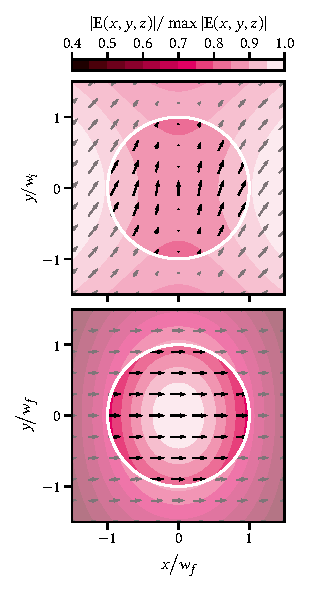
\includegraphics{img/pdf/setup/modes_2d}
    \caption[\imgsource{img/py/setup/extraction.py}]{
        Electric field at the sample surface (top) and the objective lens plane (bottom).
        The white circle indicates the area from which light can be collected, corresponding to the marginal angle $w_i = d\tan\theta_{\mr{m}}$ for the upper and $w_f = \flatfrac{\CA}{2}$ for the lower plot.
        The arrows represent the projection of the vector-valued electric field onto the $xy$-plane.
        At the interface, the polarization is mostly out-of-plane and along $y$, but in the far field, represented by the lens plane, it is almost perfectly polarized along $x$.
        The intensity profile changes from a local minimum at the center to maximal with a roughly circular dependence.
    }
    \label{fig:setup:optics:coupling:modes_2d}
\end{marginfigure}

In order to estimate the fiber coupling efficiency of the light escaping the sample and collected by the objective lens focused by the ocular lens \enquote{D}, we need to consider refraction and transmission of the electric field at the surface, collimation by the objective lens, as well as diffraction at the ocular lens aperture.
A detailed accounting of these effects is beyond the scope of this thesis.
However, let us at least gain an intuition for the degree of these effects.
Since we observe the dipole, oriented in-plane inside the \gls{qw}, from the side, it is useful to rotate the spherical coordinate system so that it is embedded in the coordinate system $(x, y, z)$ as defined in \cref{fig:setup:optics:coupling:emission} with coordinates $(r, \theta, \phi)$.

The magnitude of the electric field vector in the surface plane, which I derive in more detail in \cref{sec:app:setup:optics:modes}, is shown in the upper panel of \cref{fig:setup:optics:coupling:modes_2d}.
The circle delimits the cone of emission bounded by $\theta_\mr{m}$ (radius $w_i$) while the arrows indicate the projection of the electric field $\bvec{E}(x, y, z)$ onto the interface, indicating that the polarization in the plane points mostly along $y$ at this distance from the source.
Accounting for refraction and modifying the perpendicular and parallel ($s$ and $p$) components of the electric field according to Fresnel's equations~\cite{Hecht2017} results in the electric field in the plane of the objective lens at a distance of $\fob$ shown in the lower panel.
Here, the circle indicates the \gls{ca} of the lens with radius $w_f$.
The picture is quite different from before.
First, the field is almost exclusively polarized along $x$, the dipole axis, as we might have expected.
Moreover, the intensity $\propto\abs{\bvec{E}}^2$ does not depend strongly on the azimuthal angle $\phi$ at this distance, allowing us to approximate the field as rotationally invariant to estimate the coupling efficiency into the \gls{smf}.\sidenote[][*4]{
    Note that, while a fairly good approximation for the amplitude, this is likely not a good approximation for the phase because $k w_i \sim 1$, meaning that when the light exits the sample the phase is not constant across the surface, and the approximation as a point source just below the surface emitting a spherical wave warrants further investigation, \cf \cref{sec:app:setup:optics:modes}.
}
As shown in \cref{sec:app:setup:optics:modes}, the field after collimation is thus to good approximation given by
\begin{equation}\label{eq:setup:optics:coupling:efield:lens}
    \bvec{E}(r, \theta) = \tilde{A}(r)E_x(\theta)
\end{equation}
with
\begin{align}
    \tilde{A}(r) &= \frac{\abs{\bvec{p}}k^2}{4\pi\epsilon}\frac{\exp(\i k z)}{r} \\
    E_x(\theta) &= \frac{2n\pi\cos\theta\left[\cos\theta + n\nu(\theta) + n\nu(\theta)\cos\theta + \nu(\theta)^2\right]}{[n\cos\theta + \nu(\theta)][\cos\theta + n\nu(\theta)]} \label{eq:setup:optics:coupling:efield:lens:x}
\end{align}
and where $\nu(\theta) = \sqrt{1 - n^2\sin^2\theta}$.
For $\tilde{A}(r)$, we assumed a perfect lens that transforms a spherical wave front with constant phase at constant $r$ into a plane wave with constant phase at constant $z$.

\begin{marginfigure}[*-2]
    \centering
    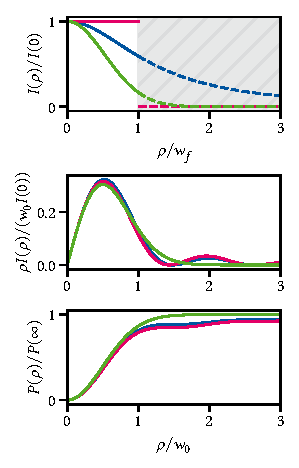
\includegraphics{img/pdf/setup/modes_1d}
    \caption[\imgsource{img/py/setup/extraction.py}]{
        Electric field modes.
        Top: mode intensity of the light collected from the semiconductor at the objective lens plane (blue) in comparison to a flattop (magenta) and Gaussian \TEM{00} mode with theoretical beam diameter after collimating with the ocular lens (green).
        $w_f$ is the lens \gls{ca} radius.
        Middle: diffraction pattern of the collimated beam when focusing onto the \gls{smf} end face with the ocular lens (blue), the flattop approximation (magenta), and the fiber's guiding mode (green).
        The curves are scaled with the radial coordinate $\rho$ to highlight the Airy rings.
        Bottom: power encased by a circle with radius $\rho$, $P(\rho)\propto\int_0^{\rho}\dd{\rho^\prime} \rho^{\prime} I(\rho^{\prime})$.
    }
    \label{fig:setup:optics:coupling:modes_1d}
\end{marginfigure}

The radial intensity profile ($\rho = \fob\tan\theta$ and $r=\sqrt{\rho^2 + \fob^2}$) given by the absolute value square of \cref{eq:setup:optics:coupling:efield:lens} is shown in the upper panel of \cref{fig:setup:optics:coupling:modes_1d} together with a flattop (magenta) and a Gaussian (green) beam profile for comparison.
The intensity drops to about half its maximum at the edge of the lens aperture, $\rho=w$.
We may thus expect the mode matching to be qualitatively different from the flattop behavior discussed previously when coupling this beam into a \gls{smf} with a guiding mode very closely approximating the Gaussian \TEM{00} mode.

The light collected and collimated by the objective lens next passes through the ocular lens in the detection arm which focuses it into the \gls{smf}.
The image of the beam on the fiber end face is given by the Fraunhofer diffraction pattern generated by the wave (\cref{eq:setup:optics:coupling:efield:lens}) incident on the ocular lens aperture, which I give in \cref{sec:app:setup:optics:diffraction}.
The resulting diffraction pattern, \cref{eq:app:setup:optics:diffraction}, scaled with the radius $\rho$ is plotted in the middle panel of \cref{fig:setup:optics:coupling:modes_1d} together with the corresponding Airy disk result for a flattop beam (\cref{eq:setup:optics:coupling:flattop:diffraction_pattern}) and the \gls{smf}'s guiding Gaussian mode.
The pattern of the flattop and the more accurate mode profile from \cref{eq:setup:optics:coupling:efield:lens} are quite similar, but noticeably differ from the Gaussian mode at higher radii $\rho$.
The lower panel shows the fraction of power included in a circle of radius $\rho$, $P(\rho)\propto \int_0^{\rho}\dd{\rho^{\prime}} \rho^{\prime} I(\rho^{\prime})$, demonstrating that we can expect the mode matching to be fairly good.
Indeed, evaluating \cref{eq:setup:optics:coupling:efficiency:mode_matching} for the light field ($E_{\mr{l}}$, \cref{eq:setup:optics:coupling:efield:lens}) and the fiber's guiding mode ($E_{\mr{g}}$, \cref{eq:setup:optics:coupling:efield:tem00}), results in
\begin{equation}\label{eq:setup:optics:coupling:efficiency:mode_matching:eval}
    \eta_{\mr{m}}(E_{\mr{l}}, E_{\mr{g}})\approx\qty{83}{\percent}
\end{equation}
for our parameters, slightly better than the naive result using the flattop beam.
Together with the collection efficiency (\cref{eq:setup:optics:coupling:efficiency:collection}) and accounting for the transmittivity of the \gls{bs}, $T\approx\qty{87}{\percent}$,\sidenote[][*3]{
    \label{sidenote:setup:optics:bs}
    While the specifications of the beamsplitter are $T\div R = \qty{90}{\percent}\div \qty{10}{\percent}$, in reality $T\div R\approx\qty{87}{\percent}\div \qty{6}{\percent}$ which also varies slightly with polarization.
}
the \emph{optical efficiency}~\cite{Sze2007} from sample to fiber is thus
\begin{equation}\label{eq:setup:optics:coupling:efficiency:optical}
    \eta_{\mr{o}} = \eta_{\mr{c}}\eta_{\mr{m}} T \approx\qty{1.0}{\percent}.
\end{equation}

\begin{margintable}[*2]
    \centering
    \footnotesize
    \begin{threeparttable}
        \caption{
            Measured efficiencies of optical elements along the detection path for laser light reflected from the sample.
            All efficiencies are with respect to the previous stage, \ie, the first row is the amount of power measured after \gls{bs}1 divided by the power entering the cryostat
        }
        \label{tab:setup:optics:efficiency:measured}
        \begin{tabularx}{\marginparwidth}{lS}
            \toprule
            \textsc{Opt. element}                   & {Efficiency (\unit{\percent})} \\
            \midrule
            Collection + \acrshort{bs}1\tnote{a}    & 37.8 \\
            Analyzer\tnote{b}                       & 67.6 \\
            Detection fiber\tnote{c}                & 39.1 \\
            Spectrometer\tnote{d}                   & 22.2 \\
            \midrule
            Total                                   & 2.2 \\
            \bottomrule
        \end{tabularx}
        \begin{tablenotes}
            \scriptsize
            \item[a] Reflected and transmitted through windows and \acrshort{bs}1
            \item[b] Transmitted through the analyzer
            \item[c] Emitted from the detection \acrshort{smf}
            \item[d] Emitted from the spectrometer side exit port
        \end{tablenotes}
    \end{threeparttable}
\end{margintable}

Due to the small intensities when dealing with \gls{pl} emitted from a membrane sample, it is difficult to measure this efficiency directly to compare it to the theoretical expectation.
What can be done rather easily is measure the reflected laser power as it is collected by the objective lens.
Together with the reflectance obtained from the calibration measurement in \cref{sec:setup:vibrations:optic}, we can then estimate the various efficiencies.
With the polarizer and analyzer co-polarized for maximum transmission and the laser $s$-polarized \wrt to \gls{bs}1 (\cf \cref{fig:setup:optics:optical_path}), I measured the efficiencies listed in \cref{tab:setup:optics:efficiency:measured}.
The \enquote{Collection + \gls{bs}1} efficiency corresponds to $Tr$ with $r$ the reflectance of the sample and matches reasonably well the expected value of $r=\abs{(n-1)/(n+1)}^2\approx\qty{32}{\percent}$ for \ch{GaAs}.
The transmittance of the analyzer (a nanoparticle linear film polarizer~\cite{ThorlabsLPVIS050-MP2}) is lower than expected from the datasheet, which quotes around \qty{80}{\percent} at \qty{800}{\nano\meter}.
Coupling into the \gls{smf} (\enquote{Detection fiber}) is significantly worse than expected from the considerations in \cref{subsec:setup:optics:coupling:lenses} for a Gaussian beam.
Since the beam used to measure the efficiencies is launched from and collimated by the same fiber type and lens as used to collect the light, the coupling efficiency should theoretically be as large as unity.
However, due to the small \gls{mfd}, alignment is tricky and vibrations may be expected to significantly reduce the coupling efficiency (\cf \cref{ch:setup:vibrations}).
It is moreover unclear how well the beam retains its Gaussian \TEM{00} mode profile after traversing the entire optical path (\cf \cref{fig:setup:optics:optical_path}).
Lastly, the throughput efficiency of the spectrometer is also lower than expected by a factor of order two.
The gratings have efficiencies on the order of \qty{50}{\percent}, and since the measurement was conducted with monochromatic light, there should be no other significant loss channels, indicating the spectrometer might not be perfectly well aligned.
To fully account for all losses, the \gls{pde} (also called \gls{qe}) of the \gls{ccd} (\ccd, $\eta_{\QE}\sim\qty{85}{\percent}$) or the \glspl{spcm} (\spcm, $\eta_{\QE}\sim\qty{65}{\percent}$) needs to be taken into account.
In summary, while certainly allowing room for improvement, the total optical efficiency of $\eta_{\mr{o,tot}} = \qty{2.2}{\percent}$ given by the power arriving at the plane of measurement -- either the \gls{ccd} or the \glspl{spcm} -- as fraction of the power incident on the cryostat is at an acceptable level.

\subsection{Imaging the laser spot}\label{subsec:setup:optics:coupling:imaging}
As the confocal microscope is free space, we are in a position to image the sample using a white light source.
We can also, though, use the imaging capabilities to inspect the laser spot focused onto the sample and compare it to the behavior expected from \cref{subsec:setup:optics:coupling:lenses}.
To this end, I coupled the laser into both excitation and detection arm of the microscope and aligned their spots on top of each other on a gold gate fabricated using optical lithography -- ensuring close to perfect reflectivity -- by monitoring their image on the \cmoscam (\cf \cref{fig:setup:optics:optical_path}).
A feature of known size, for example the width of the gate, can be used to calculate the magnification of the lens system defined by $O$ and $C$ (\cf \cref{sec:setup:vibrations:optic}).\sidenote{
    Note that this varies slightly depending on the focal distance of sample and camera from their respective lenses.
    Theoretically, we expect the magnification to be given by the ratio of their focal lengths, $M=\foc/\fob\approx\num{32}$.
}
Once aligned and blocking the beam from each arm in turn, I recorded a picture of the spots.

\begin{figure}
    \centering
    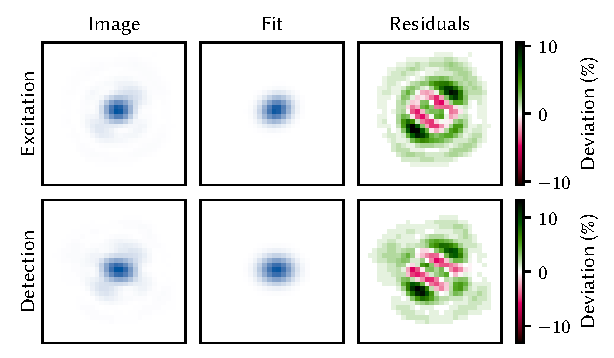
\includegraphics{img/pdf/setup/spots}
    \caption[\imgsource{img/py/setup/imaging.py}]{
        Imaging of the laser spots using the free-space imaging capabilities of the confocal microscope.
        Left column shows images of the spot on an optical gate taken with the \gls{cmos} camera, while the middle column shows the fit to \cref{eq:setup:optics:coupling:intensity:tem00} rotated by a variable amount.
        Right column shows the residuals of the fit, highlighting non-Gaussian components in the beam.
        Top row is the excitation, bottom the detection path.
    }
    \label{fig:setup:optics:coupling:imaging}
\end{figure}

From \cref{eq:setup:optics:coupling:efield:tem00}, we can deduce that a perfect, aberration-free spot would have the two-dimensional intensity distribution
\begin{equation}\label{eq:setup:optics:coupling:intensity:tem00}
    I(x, y) = I(0, 0) \exp\left\lbrace -\frac{2 x^2}{w_{0,x}^2} -\frac{2 y^2}{w_{0,y}^2} \right\rbrace,
\end{equation}
where $w_{0,\lbrace x,y\rbrace}$ are the beam waist radii in $x$ and $y$-direction, respectively, which are equal in the perfect case and introduce ellipticity else.
Allowing for ellipticity as well as a rotation of the coordinate system with respect to the axes of the \gls{cmos} camera, we can fit \cref{eq:setup:optics:coupling:intensity:tem00} to the pictures obtained previously.
The result is shown in \cref{fig:setup:optics:coupling:imaging} for the excitation path in the upper and the detection path in the lower row.
The first column shows a cropped section of the recorded images, showing good alignment between both spots but also some sidelobes along perpendicular axes rotated by around \qty{45}{\degree} to the camera axes.
This is also reflected in the relative residuals of the fitted spot that clearly shows that the spot is not described only by a Gaussian \TEM{00} mode.
However, extracting the beam waist radii from the fits and scaling with the magnification factors, which display a slight asymmetry between the two axes, \num{30} to \num{27.4}, we obtain reasonable results between \num{1.4} and \num{2} times larger than the diffraction limit given by the lens geometries, \cf \cref{subsec:setup:optics:coupling:lenses}, as shown in \cref{tab:setup:optics:coupling:imaging}.
For a more faithful measurement of the spot size one typically performs a knife-edge measurement.
This has the advantage that it does not depend on additional components of the optical path such as the beam splitter \acrshort{bs}2 and focusing lens.
In \cref{sec:setup:vibrations:optic} I perform such a measurement in the context of vibration spectroscopy.

\begin{margintable}
    \centering
    \footnotesize
    \caption{
        Beam waist radii extracted from the fits of \cref{eq:setup:optics:coupling:intensity:tem00} to the images recorded using the imaging path of the confocal microscope.
    }
    \label{tab:setup:optics:coupling:imaging}
    \begin{tabular}{lSS}
        \toprule
        \textsc{Beam waist} (\unit{\micro\meter})    & $w_{0, x}$ & $w_{0, y}$ \\
        \midrule
        Detection path                               & 0.58       & 0.75 \\
        Excitation path                              & 0.60       & 0.84 \\
        Diffraction limit                            & 0.42       & 0.42 \\
        \bottomrule
    \end{tabular}
\end{margintable}

From experience, the sidelobes present in \cref{fig:setup:optics:coupling:imaging} can be suppressed with better alignment and are most likely due to an imperfect focal distance of the fiber collimating lenses $D$ and $E$ resulting in a secondary (back) focal plane before the objective lens.
The asymmetry resulting in elliptical spot cross sections, on the other hand, might be due to several factors including a tilt of the sample or alignment of the imaging arm of the microscope.\sidenote{
    Notice that the asymmetry is due solely to the magnification factor rather than the image on the camera,
}
Finally, note that the excitation spot typically looks worse than the detection spot, likely because of the additional optical elements introducing beam distortions.

\subsection{Cross-polarization extinction}\label{subsec:setup:optics:coupling:rejection}
An essential part of the confocal microscope's design is the ability to reject the excitation laser from coupling into the detection fiber.
In a conventional microscope, this issue is avoided because one can arrange the illumination and detection lenses such that their optical axes are orthogonal and the light used for excitation of the sample does not scatter into the objective lens.
In a confocal geometry, though, the same lens is used for excitation and detection, and unwanted excitation light dominates the response unless filtered out by means of, \eg, a notch filter.
This limits the optical bandwidth of the microscope and hence other techniques are desirable.
Here, excitation rejection is achieved by cross-polarization of the polarizer (P, \polarizer) setting the polarization axis of the beam launched from the excitation \gls{smf} and the analyzer (A, \polarizer) just before coupling the light into the detection \gls{smf}.
As demonstrated by \citet{Benelajla2021}, this technique enables extinction ratios\sidenote{
    Defined as incident power over transmitted power.
}
up to \num[print-unity-mantissa=false]{1e10} in a confocal geometry, far beyond the bare polarizer extinction ratio of up to $\sim\num[print-unity-mantissa=false]{1e8}$~\cite{ThorlabsLPVIS050-MP2}.
In our case, vibrations and rough sample surfaces from which the light is reflected limit the extinction ratio to $\sim\num[print-unity-mantissa=false]{1e6}$.

As the laser beam launched from the excitation fiber is already polarized, rather than rotate the polarizer, the plane of polarization is rotated using a \halfwave plate.
To compensate for ellipticities introduced by the \gls{bs}, windows, and sample reflection, a \quarterwave plate is inserted after the \halfwave plate~\cite{Kuhlmann2013}.
The waveplates are mounted on piezoelectric rotation stages (\rotator with \rotatorcontroller controller), allowing for computer-controlled adjustment of the angles.
Previously, a third rotation stage was used to rotate the analyzer, but I found this to deteriorate the fiber coupling, most likely due to an angle-dependent beam deflection of the analyzer.\sidenote[][*-5]{
    This effect was less pronounced with the unmounted version of the same polarizer, \polarizerunmounted.
    That though introduced significant etaloning with a free spectral range of $\Delta\lambda\approx\lambda^2/2 n l\approx\qty{100}{\pico\meter}$ matching the substrate thickness of $l = \qty{2}{\milli\meter}$~\cite{Ismail2016}.
}
Furthermore, the optics behind the analyzer such as the diffraction grating have polarization-dependent properties so that it is in any case a good idea to fix the plane of polarization.
I therefore used only the waveplates on the excitation arm to fine-tune the excitation rejection, which is not ideal since the same argument as before naturally also applies to the optics behind these, such as the beam splitter whose ratio is polarization dependent.
It is hence advisable to insert another \halfwave plate on a rotation stage before the analyzer and use it together with the \quarterwave plate for rejection control.

To analyze the properties of the excitation rejection, I measured the \gls{od} as a function of the relative waveplate angles $\Delta\phi_{\halfwave(\quarterwave)}$.
The \gls{od} is defined as
\begin{equation}\label{eq:setup:optics:od}
    \OD = \log_{10}\left(\frac{P_{\mr{i}}}{P_{\mr{t}}}\right),
\end{equation}
where $P_{\mr{t}}$ is the transmitted power after and $P_{\mr{i}}$ the incident power before the analyzer.
To evaluate this expression, I measured the photon flux $\dot{\Phi}_{\mr{t}}$ after the spectrometer using the \glspl{spcm} when irradiating a sample with the laser and compared it to the power $P$ measured at the optical head.
Together with the optical efficiency $\eta_{\mr{o,tot}}$ measured in \cref{subsec:setup:optics:coupling:efficiency}, the \gls{spcm}'s \gls{pde} $\eta_{\QE}$, and the beam splitter ratio $T\div R$ (\cf \cref{sidenote:setup:optics:bs}), \cref{eq:setup:optics:od} then becomes
\begin{equation}\label{eq:setup:optics:od:eval}
    \OD = \log_{10}\left(\frac{P\times\flatfrac{R}{T}}{\flatfrac{hc}{\lambda}\times\dot{\Phi}_{\mr{t}}/\eta_{\mr{o,tot}}\eta_{\QE}}\right).
\end{equation}

\begin{figure}
    \centering
    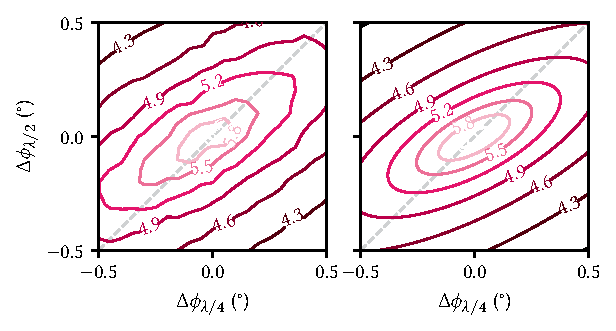
\includegraphics{img/pdf/setup/rejection}
    \caption[\imgsource{img/py/setup/excitation_rejection.py}]{
        \Gls{od} measured (left) and fitted (right) as function of relative \quarterwave and \halfwave angles.
        The dashed gray line indicates the axis along which there should be no dispersion if all optics between polarizer and analyzer were polarization-independent.
    }
    \label{fig:setup:optics:rejection}
\end{figure}

\Cref{fig:setup:optics:rejection} shows the measurement when the laser was focused on an exciton trap (\cf \cref{part:exp}) in the left panel.
The dashed gray line indicates the axis along which the \gls{od} should theoretically be constant (rotating the \halfwave plate changes the plane of polarization, so the \quarterwave plate should need to be rotated by the same amount to retain a constant angle between plane of polarization and fast axis of the waveplate).
The \gls{od} reaches maximum values around \num{6.4} -- corresponding to an extinction ratio of \num{2.5e6} -- but quickly falls off by more than an order of magnitude even for small angular displacements.\sidenote{
    The maximum achievable \gls{od} depends strongly on the sample surface off which the laser is reflected, see also \citer{Kumar2016a}.
}
Qualitatively, one finds that close to the extinction maximum, the count rate $\dot{\Phi}_{\mr{t}}$ is a rotated paraboloid of the form
\begin{equation}
    \dot{\Phi}_{\mr{t}} = \bvec{a}\transpose\bvec{\Delta\tilde{\phi}}^2 + \dot{\Phi}_0
\end{equation}
with $\bvec{\Delta\tilde{\phi}} = R(\pi/4+\theta)\bvec{\Delta\phi}$, $\bvec{\Delta\phi} = (\Delta\phi_{\quarterwave},\Delta\phi_{\halfwave})\transpose$, and $R(\theta)$ a rotation matrix.
Inserting into \cref{eq:setup:optics:od:eval} yields
\begin{equation}\label{eq:setup:optics:od:fit}
    \OD = \log_{10}\left(\frac{P R\lambda\eta_{\mr{o,tot}}\eta_{\QE}}{h c}\right) - \log_{10}(\bvec{a}\transpose\bvec{\Delta\tilde{\phi}}^2 + \dot{\Phi}_0),
\end{equation}
a fit to which is shown in the right panel of \cref{fig:setup:optics:rejection}, displaying good agreement with the data.
From the fit, we extract $\theta=\qty{-17}{\degree}$, indicating a non-negligible polarization dependence, as well as quadratic dispersion coefficients $\partial^2\OD/\bvec{\Delta\tilde{\phi}}^2=\qty[per-mode=symbol]{-0.16}{\per\milli\textdegree\squared}$ and \qty[per-mode=symbol]{-0.02}{\per\milli\textdegree\squared} perpendicular (parallel) to the axis along $\flatfrac{\pi}{4}+\theta$, respectively.

The optics between polarizer and analyzer furthermore display chromatic dispersion.
When changing the excitation wavelength, the angles of \halfwave and \quarterwave plate therefore need to be re-optimized.
I describe the automatic calibration procedure implemented in the measurement framework to this end in \cref{part:exp}.

\section{Exemplary measurement of non-classical light}\label{sec:setup:optics:g2}
As a demonstration of the optical capabilities of the setup, I performed second-order coherence measurements of an \ch{InAs} \gls{saqd} in \ch{GaAs}.
\Glspl{saqd} are \glspl{oaqd} that form at random locations during epitaxial growth.
They have demonstrated excellent optical properties and show potential for technological applications such as quantum repeaters~\cite{Petroff2001,Warburton2013,Lodahl2015,Zajac2025}.
In particular, \glspl{saqd} can be operated as single-photon sources.
Because they locally deform the band structure, they can capture and confine excitons.
Owing to their small spatial extents, strong Coulomb interaction shifts the energy of excitonic complexes other than the neutral exciton $X^{0}$, implying that light emitted at $h\nu = E_{X^{0}}$ upon recombination is certain to contain a single photon within a time window on the scale of the exciton lifetime.
This so-called photon \emph{anti-bunching} behavior\sidenote{
    Also known as sub-Poissonian statistics.
}
can be measured with a \gls{hbt} interferometer and serves as a fingerprint of single-photon source behavior.

\begin{marginfigure}
    \centering
    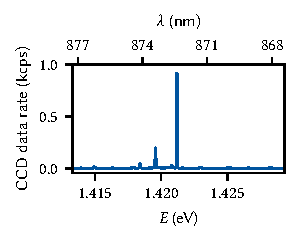
\includegraphics{img/pdf/setup/ingaas_pl}
    \caption[\imgsource{img/py/setup/g2.py}]{
        \Gls{pl} spectrum of a \gls{saqd} under \gls{cw} excitation at \qty{793}{\nano\meter}.
    }
    \label{fig:setup:optics:ingaas:pl}
\end{marginfigure}

I loaded and cooled down an \ch{InAs/GaAs} chip with \glspl{saqd} and selected a bright and isolated emission line.
A typical \gls{pl} spectrum under \gls{cw} above-gap excitation is shown in \cref{fig:setup:optics:ingaas:pl}.
The brightest line at $\qty{1.4212}{\eV} = \qty{872.39}{\nano\meter}$ has a width of around $\qty{15}{\micro\eV} = \qty{12}{\pico\meter}$ close to the grating\sidenote{
    \qty{1800}{lines\per\milli\meter}, resulting in a dispersion of $\dv*{\lambda}{x} = \qty{325}{\pico\meter\per\milli\meter}$ in the focal plane.
}
resolution limit of around \qty{5}{pm}.
To perform a \g2 experiment, light emitted by the source is spectrally filtered using the \spectrometer diffraction grating spectrometer and sent through a 50:50 \gls{bs} with a \spcm \gls{spcm} on each exit port.
The clicks from the detectors are time-correlated using a counting card (\tagger), computing the second-order coherence function~\cite{Kimble1976,Walls1979,Cohen-Tannoudji1998}
\begin{equation}
    \g{2}(\tau) = \frac{\expval{\hat{n}_1(t)\hat{n}_2(t + \tau)}}{\expval{\hat{n}_1(t)}\expval{\hat{n}_2(t)}},
\end{equation}
where $\hat{n}_i(t) = \hat{b}^\dagger_i(t) \hat{b}_i(t), i\in\lbrace 1,2\rbrace$ is the photon-number operator for a single mode at detector $i$ and averaging takes place over time.
For a weakly excited artificial atom, one expects this function to take on the form~\cite{Walls1979}
\begin{equation}\label{eq:setup:optics:g2:fit}
    \g{2}(\tau) = \left[1 - \exp(-\flatfrac{\tau\gamma}{2})\right]^2,
\end{equation}
where $\gamma$ is the Einstein $A$ coefficient, \ie, the spontaneous emission rate or inverse lifetime $1/T_1$ of the excited state.

\begin{marginfigure}
    \centering
    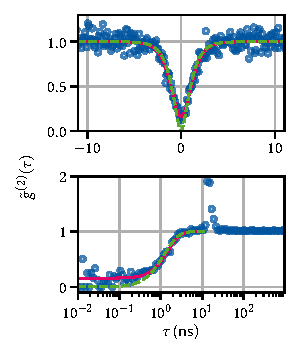
\includegraphics{img/pdf/setup/ingaas_g2}
    \caption[\imgsource{img/py/setup/g2.py}]{
        \g{2} measurement of the emission line at \qty{872.267}{\nano\meter} under \gls{cw} excitation with \qty{1}{\micro\watt} at \qty{793}{\nano\meter}.
        The monochromator bandwidth was $\Delta\lambda = \qty{200}{\pico\meter} = \qty{325}{\micro\eV}$.
    }
    \label{fig:setup:optics:ingaas:g2}
\end{marginfigure}

The upper panel of \cref{fig:setup:optics:ingaas:g2} shows the measurement after a total run time of around \qty{17}{\hour} together with a fit to \cref{eq:setup:optics:g2:fit} from which we extract a lifetime of $\gamma\inverse = \qty{430+-11}{\pico\second}$.
$\g2(0)$ does not quite reach the theoretically expected value of zero.
Likely causes include the remnant dark counts of the detectors\sidenote{
    On the order of \qty{50}{cps} each.
    The average count rate during the experiment was $\sim\qty{5.5}{\kilo cps}$ and \qty{5.9}{\kilo cps}.
}
and additional decay channels.
The lower panel shows the same measurement for logarithmically spaced time lags $\tau$ covering a wider range.
A peculiar feature shows at $\tau = \qty{13.4}{\nano\second}$, where the measurement suggests a bunching of photons with $\g2(\tau) \approx 2$.
The origin of this bump is not understood.
One possible cause might be multiple reflections in the setup.
However, in free space the delay corresponds to a time-of-flight distance of \qty{4}{\meter}, far larger than any distances in the setup besides the path between objective and ocular lens at $\sim\qty{1.5}{\meter}$.
Assuming a refractive index of $n=\num{1.4}$ for a typical \gls{smf} results in a characteristic distance of \qty{2.8}{\meter} which also does not match any components in the setup.\sidenote{
    The closest match is the \qty{10}{\meter} fiber from the optical head to the optical table.
}
What can be said is that it is related to the setup rather than a physical process in the sample since the feature also appeared in \g2 measurements on different samples.
For measurements such as the one performed here, though, this effect may safely be treated as a measurement artefact and ignored.
Only in case the characteristic decay time $\gamma\inverse$ approached \qty{10}{\nano\second} this would need to be investigated more carefully.
Finally, I note that the dependence of the integrated peak power on excitation power for this line was superlinear, suggesting an excitonic complex rather than the natural exciton as the source of emission.
The line at \qty{1.4196}{\eV} did show a linear relationship and produced qualitatively the same \g2 results.

% mainfile: ../../main.tex
\chapter{Vibration noise}\label{ch:setup:vibrations}
\AutoLettrine{A} microscope's performance is limited chiefly by two factors; first and foremost the resolution and imaging fidelity are limited by the systematic aberrations introduced by the optics.\sidenote{
    Besides the limit set by the wavelength-dependent diffraction, of course.
}
Various types of aberrations exist, and modern microscopes usually include a complex assembly of optics to compensate for these errors.
The second factor is vibration noise.
This becomes more significant the higher the resolution of the microscope simply because ambient, environmental vibrations within the range of human civilization are typically on the order of $\qty{100}{\micro\meter\per\second}$ \gls{rms}~\cite{Gordon1999}.
Comparing that to transmission electron microscopes with atomic resolution, it is clear that these instruments require purpose-built rooms to reduce the vibration level to acceptable levels.

The demands on the microscope discussed in \thethesis are fortunately much more relaxed as the features we need to resolve are on the micrometer scale.
However, we face the additional challenge of ultra-low temperatures, or rather the manner in which they are achieved.
The microscope is integrated into a \emph{dry} \gls{dr}.
In contrast to a \emph{wet} \gls{dr}, which uses a liquid Helium bath, these systems achieve the pre-cooling necessary for the \ch{^3He}/\ch{^4He} dilution refrigeration cycle to work by adding a secondary refrigeration mechanism, usually a \gls{ptr}.
These are closed-cycle systems that work with \ch{^4He} compressed to \textasciitilde\qty{21}{\bar} on the high-pressure and \textasciitilde\qty{7}{\bar} on the low-pressure side.
A rotating valve connecting high and low pressure lines to the cryostat in turn produces alternating gas flow inside a regenerator, where the gas absorbs heat at the low-temperature and and deposits heat at the high-temperature end~\cite{Radebaugh2009,DeWaele2011}.
In commercial \glspl{ptr} the frequency of the pulses of Helium gas, determined by the rotary valve motor, is usually fixed at values around \qty{1.5}{\hertz}.

Naturally, the compressor, the rotary valve motor, and the Helium pulses themselves introduce vibrations into the cryostat.
While the cold foot of the \gls{ptr} is not rigidly connected to the cryostat interior,\sidenote{
    In the \odin copper braids connect the cold head to the \gls{pt1} and \gls{pt2} plates.
    There exist commercial systems that use gas exchange instead, for example the \mbox{CryoConcept} HEXA-DRY series~\cite{CryoConceptHexaDry}.
}
the entire cold head assembly rests with rubber feet on the cryostat top plate in the system's delivery status.
Thus, our microscope does not only encounter passive environmental vibrations but also the active perturbation from the \gls{ptr}.

Several authors have addressed vibration decoupling in \glspl{ptr}.
\citet{Caparrelli2006} employed active control of a sample stage at \qty{3}{\kelvin} to attenuate vibrations.
\citet{Pelliccione2013,Oh2021,Esser2024} constructed scanning gate microscopes in \gls{ptr}-cooled systems, demonstrating excellent displacement noise.
\citet{Kalra2016} investigated the impact of \gls{ptr}-vibrations on electrical noise while \citet{Riabzev2009,Olivieri2017,Schmoranzer2019} investigated the generation and decoupling of vibrations.
Due to space constraints, the complexity of decoupling solutions we can apply to our microscope is limited.
Nonetheless, I show in the following chapter that the rigid-body construction of the optics together with passive air spring damping reduces the vibration noise to an adequate level for our purposes.

This chapter is laid out as follows.
In \cref{sec:setup:vibrations:isolation}, I briefly discuss the theoretical underpinnings of vibration isolation to inform its optimization.
To characterize and improve upon the isolation, I performed vibration noise spectroscopy using the techniques and tools presented in \cref{part:speck}.
I employed two different approaches that I lay out in the following; first, using a commercial piezoelectric accelerometer (\cref{sec:setup:vibrations:accel}) and second, using the optical response of a spatial reflectance gradient (\cref{sec:setup:vibrations:optic}).
As will become clear, the two approaches complement each other because they are sensitive to slightly different quantities.

\section{Vibration isolation}\label{sec:setup:vibrations:isolation}
A simple yet effective method of vibration isolation is to suspend the system on passive air springs.
These are typically constructed with two separate air chambers, a spring and a damping chamber, connected by pneumatic tubing.
The load is rigidly mounted to a plunger that rests on a diaphragm sealing the spring chamber.
Excitations of the load induce oscillations in the variable spring chamber volume.
The connection to the fixed-volume damping chamber provides a flow impedance\sidenote{
    The speed of a fluid in laminar flow through a round pipe is proportional to the pressure gradient along the flow direction and to the square of the distance from the wall.
}
that manifests as a damping force to the spring chamber oscillations.

\subsection{Damping theory}\label{subsec:setup:vibrations:isolation:theory}

\begin{marginfigure}
    \centering
    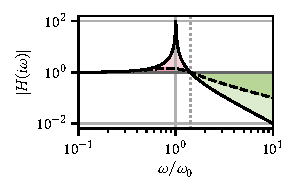
\includegraphics{img/pdf/setup/spring_tf}
    \caption[\imgsource{img/pdf/setup/springs.py}]{
        Force transmission function of a damped harmonic oscillator with $\gamma=\omega_0/100$ (solid black line) and $\gamma=\omega_0/2$ (dashed black line).
        Below the break frequency $\omega=\sqrt{2}\omega_0$ (dotted vertical line), external excitations are amplified (shaded red area).
        For larger damping $\gamma$, the amplification at resonance becomes smaller.
        Above $\omega=\sqrt{2}\omega_0$, excitations are attenuated (shaded green area).
        Both amplification below and attenuation above the break frequency become smaller as the damping rate $\gamma$ is increased.
    }
    \label{fig:setup:vibrations:spring:tf}
\end{marginfigure}

Let us adopt a simple toy model to gain an intuition for the behavior of a mass suspended on air springs as function of vibration frequency by modelling it as a damped harmonic oscillator.
Consider the displacement from equilibrium $x(t)$ of the test mass $m$ and switch on an external perturbation $u(t)$ acting on the \emph{base} of the spring, implying that the driving force experiences both the damping rate $\gamma$ and the spring stiffness $k=m\omega_0^2$ with $\omega_0$ the resonant frequency of the undamped system.
We can then compute the transfer function $H(s)$ from the Laplace transform of the Newtonian equation of motion,
\begin{equation}\label{eq:setup:spring:eom}
    \ddot{x}(t) + 2\gamma[\dot{x}(t)-\dot{u}(t)] + \omega_0^2 [x(t)-u(t)] = 0,
\end{equation}
yielding
\begin{equation}\label{eq:setup:spring:tf}
    H(s) = \frac{\hat{x}(s)}{\hat{u}(s)} = \frac{2\gamma s + \omega_0^2}{s^2 + 2\gamma s + \omega_0^2}.
\end{equation}
The magnitude of the transfer function evaluated at $s=\i\omega$ is shown in \cref{fig:setup:vibrations:spring:tf} for two different dampings, $\gamma = \omega_0/200$ (solid black line) and $\gamma = \omega_0/2$ (dashed black line).
Below $\omega=\sqrt{2}\omega_0$ (vertical dotted line), external impulses are in fact amplified.
The maximum at the damped system's resonance $\omega_{\mr{r}} = [\omega_0^2 - \gamma^2]^{\flatfrac{1}{2}}$ becomes smoothed out and smaller as the damping $\gamma$ is increased but never drops below unity.
This is the reason why resonance frequencies as small as possible are desirable in vibration isolation.
Above this frequency, the system initially attenuates with \qty{40}{\decibel} per decade up to $\omega=\omega_0^2/(2\gamma)$ and with \qty{20}{\decibel} per decade beyond for $\gamma/\omega_0\to 0$ (the underdamped case).
In the strongly damped case ($\gamma/\omega_0\to\infty$) the attenuation is only \qty{20}{\decibel} per decade starting at $\omega = 2\gamma$.

From \cref{eq:setup:spring:tf,fig:setup:vibrations:spring:tf}, we can infer two possible approaches to isolating a mass from vibrations.
The first is to make the system's resonance frequency $\omega_0$ as small as possible by resting it on a spring damping system.
This maximizes the region in which external influences are attenuated.
The second is to do the opposite, \ie, make the entire system as stiff (large $k$) and thereby $\omega_0$ as large as possible.
While this minimizes the attenuation region, it also moves the amplification region close to the resonance to higher frequencies, and possibly further away from the external excitation.
Consequently, this approach makes most sense if it is known that low-frequency excitations are the dominant source of vibrations.

A widely used metric for the isolation demand of vibration-sensitive equipment are the so-called \gls{vc}~\cite{Gordon1992,Gordon1999}.
These are design standard specifications for buildings housing, for example, lithography tools.
The \glspl{vc} are defined in terms of band-limited \gls{rms} values similar to what we have employed in \cref{part:speck} (\cf \cref{eq:setup:vibrations:rms,eq:speck:psd:bandpower}).
However, instead of computing the band-limited \gls{rms} with a fixed lower band edge, one uses bands of a fixed width, typically over one-third of an octave.
To be specific, the one-third octave is defined in terms of its midband frequency $f_{\mr{m}}$ as the interval
\begin{equation}\label{eq:setup:vibrations:third_octave}
    f\in f_{\mr{m}}\times\left[10^{-\flatfrac{1}{20}},10^{\flatfrac{1}{20}}\right] \approx f_{\mr{m}}\times\left[2^{-\flatfrac{1}{6}},2^{\flatfrac{1}{6}}\right]
\end{equation}
whose bandwidth \df is approximately \qty{26}{\percent} larger than $f_{\mr{m}}$ and where the latter is defined referenced to \qty{1000}{\hertz}~\cite{ansi_octave_bands}.
The $\flatfrac{1}{3}$ octave band \gls{rms} is then given by
\begin{equation}\label{eq:setup:vibrations:octave_band_rms}
    \rms_{\flatfrac{1}{3}\,\mr{oct.}}(f_{\mr{m}}) = \sqrt{\int_{f_{\mr{m}}/10^{1/20}}^{f_{\mr{m}}\times 10^{1/20}}\dd{f}S(f)},
\end{equation}
where $S(f)$ is the noise \gls{psd} (see \cref{ch:speck:theory}).
The criteria, given as velocities rather than displacements or accelerations because it is argued that the limit to photolithography resolution is image velocity, are reproduced from \citer{Gordon1999} in \cref{tab:setup:vibrations:vc}.
For the typical feature sizes we would like our microscope to resolve, the \acrshort{vc}-B criterion is a fair target.
I will use them below to classify the vibration isolation of the confocal microscope.

\begin{margintable}[*-13]
    \centering
    \footnotesize
    \caption{\Glspl{vc} and \acrshort{iso} guidelines~\cite{Gordon1999}.}
    \label{tab:setup:vibrations:vc}
    \begin{tabular}{ c @{}S@{} }
        \toprule
        \multicolumn{2}{l}{$\flatfrac{1}{3}$ \textsc{octave band \gls{rms} (\unit{\micro\meter\per\second})}} \\
        \midrule
        Workshop (\acrshort{iso})        & 800  \\
        Office (\acrshort{iso})          & 400  \\
        Residential day (\acrshort{iso}) & 200  \\
        Op. theater (\acrshort{iso})     & 100  \\
        \acrshort{vc}-A                  & 50   \\
        \acrshort{vc}-B                  & 25   \\
        \acrshort{vc}-C                  & 12.5 \\
        \acrshort{vc}-D                  & 6    \\
        \acrshort{vc}-E                  & 3    \\
        \bottomrule
    \end{tabular}
\end{margintable}

\subsection{Microscope isolation concept}\label{subsec:setup:vibrations:isolation:concept}
What does this mean for our case of a dry \gls{dr}?
The rotary valve motor of the \gls{ptr} generates pulses with frequency \qty{1.4}{\hertz}.
Commercial damping systems that the space constraints in our lab allow to be accommodated, for example the CFM Schiller MAS 25~\cite{CFMSchiller}, have resonance frequencies around $f_0 = \qty{2.5}{\hertz}$, implying the first two harmonics of the \gls{ptr} excitation fall into the amplification regime as discussed above.
We are thus right in-between the two regimes and it is a-priori unclear which isolation scheme to choose without detailed mechanics simulations.
Hence, the initial isolation concept for the cryostat envisaged mounting the rotary valve motor rigidly to the stiff aluminium item profile frame, which was additionally filled with sand to increase the system's resonance frequency.

However, prompted by a sudden increase in visually observed vibrations in the microscope image, I modified the cryostat frame to house three air springs~\sidecite{CFMSchiller} in the hopes of isolating the microscope from external disturbances.\sidenote{
    As it turned out, the cause was a damaged nanopositioner bearing rather than environmental.
    Fortuitiously, the endeavour still proved successful and resulted in an improved vibration performance as I show below.
}
To this end, I decoupled the frame from which the cryostat itself is suspended from the support frame resting on the lab ground as sketched in \cref{fig:setup:vibrations:suspension}.
Extruding from the square footprint of the support frame at two adjacent corners and the center of the diametrically opposite side, the three air springs are mounted with the base on angle brackets connected to the support frame while their plunger is mounted to a second angle bracket connected to the cryostat frame.
The springs are connected by pneumatic tubing to a central pressure regulation panel that is connected to the building's central air pressure line.
The vertical placement of the springs is chosen such that when the air springs are deflated the cryostat frame rests on the support frame, establishing the same rigid connection that existed previously.
This allows examining the influence of the air springs on the vibration isolation without modifying the setup by simply venting the pressurized air from the springs.

\begin{marginfigure}[*-7]
    \centering
    \begin{tikzpicture}[x=1cm,y=1cm,line cap=butt,line join=miter]

    %--------------------------------
    % Styles
    %--------------------------------
    \tikzset{
        frame/.style  ={line width=0.8},
        bracket/.style={line width=0.8},
        brace/.style  ={line width=0.6},
        spring/.style ={line width=0.8, decorate, decoration={zigzag,segment length=4pt,amplitude=1.2pt}},
        springGuides/.style={line width=0.5, draw=RWTHblack75, densely dotted},
        cryo/.style   ={line width=0.7, color=RWTHblack75},
        hidden/.style ={dash pattern=on 2pt off 1.3pt, color=RWTHblack75},
        groundline/.style={line width=0.6},
        hatch/.style={thin}
    }

    %--------------------------------
    % Parameters (match your current drawing)
    %--------------------------------
    \def\W{2.5}      % total width
    \def\Hlow{4.0}   % lower frame outer height
    \def\BW{0.4}     % frame wall thickness (both frames)
    \def\Gap{0.5}    % vertical gap between frames
    \def\Hup{1.5}    % upper frame outer height

    \def\Bext{0.7}   % bracket extension
    \def\Bv{0.7}     % bracket vertical leg length
    \def\Bth{0.1}    % bracket leg thickness

    % Cryostat envelope (rectangle in 2D)
    \def\CxL{0.6}    % left x of cryostat
    \def\CxR{1.9}    % right x of cryostat
    \def\Cpt{0.2}    % top plate thickness
    \def\CyBot{1.6}  % cryostat bottom y

    % Key coordinates
    \coordinate (Llow) at (0,\Hlow);
    \coordinate (Lup)  at (0,\Hlow+\Gap);
    \coordinate (Rlow) at (\W,\Hlow);
    \coordinate (Rup)  at (\W,\Hlow+\Gap);

    %--------------------------------
    % Ground (line + simple hatch)
    %--------------------------------
    \draw[groundline] (-\Bext,0) -- (\W+\Bext,0);
    \foreach \i in {0,...,13}{
        \draw[hatch] ({-\Bext+0.3*\i},0) -- ({-\Bext-0.3+0.3*\i},-0.3);
    }

    %--------------------------------
    % Lower frame
    %--------------------------------
    \draw[frame] (0,0) rectangle (\W,\Hlow);
    \draw[frame] (\BW,0) rectangle (\W-\BW,\Hlow-\BW);

    %--------------------------------
    % Upper frame
    %--------------------------------
    \draw[frame] (0,\Hlow+\Gap) rectangle (\W,\Hlow+\Gap+\Hup);
    \draw[frame] (\BW,\Hlow+\Gap+\BW) rectangle (\W-\BW,\Hlow+\Gap+\Hup-\BW);

    %--------------------------------
    % Left brackets (L-angles) and spring
    %--------------------------------
    % Lower left bracket
    \draw[bracket]
    ($(Llow)+(-\Bext,0)$) -- (Llow) -- ++(0,-\Bv) -- ++(-\Bth,0)
    -- ++(0,\Bv-\Bth) -- ++(-\Bext+\Bth,0) -- cycle;
    \draw[brace] ($(Llow)+(-\Bext+\Bth,-\Bth)$) -- ($(Llow)+(-\Bth,-\Bv+\Bth)$);

    % Upper left inverted bracket
    \draw[bracket]
    ($(Lup)+(-\Bext,0)$) -- (Lup) -- ++(0,\Bv) -- ++(-\Bth,0)
    -- ++(0,-\Bv+\Bth) -- ++(-\Bext+\Bth,0) -- cycle;
    \draw[brace] ($(Lup)+(-\Bext+\Bth,\Bth)$) -- ($(Lup)+(-\Bth,\Bv-\Bth)$);

    % Left spring: end plates + zigzag + dashed guides
    \draw[frame] ($(Llow)+(-\Bext+\Bth,0)$) -- ($(Llow)+(-\Bth,0)$);
    \draw[frame] ($(Lup)+(-\Bext+\Bth,0)$) -- ($(Lup)+(-\Bth,0)$);
    \draw[spring] ($(Llow)+(-\Bext+0.34,0)$) -- ($(Lup)+(-\Bext+0.34,0)$);
    \draw[springGuides] ($(Llow)+(-\Bext+\Bth,0)$) -- ($(Lup)+(-\Bext+\Bth,0)$);
    \draw[springGuides] ($(Llow)+(-\Bth,0)$) -- ($(Lup)+(-\Bth,0)$);

    %--------------------------------
    % Right brackets (mirror) and spring
    %--------------------------------
    % Lower right bracket
    \draw[bracket]
    ($(Rlow)+(\Bext,0)$) -- (Rlow) -- ++(0,-\Bv) -- ++(\Bth,0)
    -- ++(0,\Bv-\Bth) -- ++(\Bext-\Bth,0) -- cycle;
    \draw[brace] ($(Rlow)+(\Bext-\Bth,-\Bth)$) -- ($(Rlow)+(\Bth,-\Bv+\Bth)$);

    % Upper right inverted bracket
    \draw[bracket]
    ($(Rup)+(\Bext,0)$) -- (Rup) -- ++(0,\Bv) -- ++(\Bth,0)
    -- ++(0,-\Bv+\Bth) -- ++(\Bext-\Bth,0) -- cycle;
    \draw[brace] ($(Rup)+(\Bext-\Bth,\Bth)$) -- ($(Rup)+(\Bth,\Bv-\Bth)$);

    % Right spring: end plates + zigzag + dashed guides
    \draw[frame] ($(Rlow)+(\Bth,0)$) -- ($(Rlow)+(\Bext-\Bth,0)$);
    \draw[frame] ($(Rup)+(\Bth,0)$) -- ($(Rup)+(\Bext-\Bth,0)$);
    \draw[spring] ($(Rlow)+(0.34,0)$) -- ($(Rup)+(0.34,0)$);
    \draw[hidden] ($(Rlow)+(\Bth,0)$) -- ($(Rup)+(\Bth,0)$);
    \draw[hidden] ($(Rlow)+(\Bext-\Bth,0)$) -- ($(Rup)+(\Bext-\Bth,0)$);

    %--------------------------------
    % Cryostat (front edges solid, hidden edges dashed)
    %--------------------------------
    % Hidden edges behind upper frame web
    \draw[hidden] (\CxL,\Hlow+\Gap) -- (\CxL,\Hlow+\Gap+\BW);
    \draw[hidden] (\CxR,\Hlow+\Gap) -- (\CxR,\Hlow+\Gap+\BW);

    % Top plate
    \draw[cryo] (\CxL,\Hlow+\Gap+\BW) -- ++(0,\Cpt) -- ++(\CxR-\CxL,0) -- ++(0,-\Cpt);

    % Visible front edges down to top of lower frame
    \draw[cryo] (\CxL,\Hlow+\Gap) -- (\CxL,\Hlow);
    \draw[cryo] (\CxR,\Hlow+\Gap) -- (\CxR,\Hlow);

    % Hidden through lower frame web
    \draw[hidden] (\CxL,\Hlow) -- (\CxL,\Hlow-\BW);
    \draw[hidden] (\CxR,\Hlow) -- (\CxR,\Hlow-\BW);

    % Visible down to near floor
    \draw[cryo] (\CxL,\Hlow-\BW) -- (\CxL,\CyBot);
    \draw[cryo] (\CxR,\Hlow-\BW) -- (\CxR,\CyBot);
    \draw[cryo] (\CxL,\CyBot) -- (\CxR,\CyBot);

    % Small bottom features (optional)
    \draw[cryo] (\CxL+0.1,\CyBot) rectangle ++(0.2,-0.4);
    \draw[cryo] (\CxR-0.1,\CyBot) rectangle ++(-0.2,-0.4);

\end{tikzpicture}
    \caption[\imgsource{img/tikz/setup/suspension.tex}]{
        Sketch of the cryostat suspension.
        There are two separate frames (thick black lines), the upper of which the cryostat (grey outline) is attached to.
        The frames are connected by air springs mounted on angle brackets extruding from the frames.
    }
    \label{fig:setup:vibrations:suspension}
\end{marginfigure}

In the following, I will characterize the performance of the system with and without the air springs active using two different methods.

\section{Accelerometric vibration spectroscopy}\label{sec:setup:vibrations:accel}
The most straightforward method of measuring vibration noise is an accelerometer.
These are devices that convert translational forces, for example by means of a loaded spring, into electrical signals.
They are mounted rigidly to the \gls{dut} and typically connected to some sort of signal conditioner providing a constant current bias to the sensor and putting out a voltage proportional to the acceleration.
The most sensitive and low-frequency designs use piezoelectric materials like Quartz crystals for sensitivities in the range of \qty{10}{\volt\per\gaccel} with a broadband noise floor of \qty{2}{\micro\gaccel}~\cite{WilcoxonAccel}.

In order to evaluate the vibration level at the sample position, I designed a small angle bracket onto which the accelerometer\sidenote{
    \accelerometer kindly lent by Marcus Eßer~\cite{WilcoxonAccel}.
}
can be screwed either in vertical or horizontal direction in the sample puck of the \gls{dr}, enabling measurements of the displacement noise along the direction of gravity as well as perpendicular to it and the optical axis.
The accelerometer is connected to the coaxial cables installed in the cryostat via an adapter cable from imperial 10-32 to \acrshort{sma} connector.
Outside of the cryostat, the signal is routed to a signal conditioner that provides the necessary current bias and outputs a voltage which is digitized by a \thedmm \gls{dmm} connected to the measurement computer.
Since the sensor's (conditioned) output is a voltage directly proportional to the acceleration, it is straightforward to compute the displacement \gls{psd} from time series data measured with the \gls{dmm} using the \pyspeck package presented in \cref{ch:speck:software}~\cite{Hangleiter_pyspeck}.
Leveraging the \code{fourier_procfn} argument, we can transform the voltage data first to acceleration and then, by integration, to displacement in frequency space as indicated in \cref{lst:setup:vibrations:accel}.

\begin{marginlisting}[*-11]
    \begin{pycode}[
        fontsize=\footnotesize,
        breaklines,%
        breakafter=.,%
    ]
        from qutil.signal_processing import fourier_space
        from qutil.functools import chain, scaled
        from qutil import const

        sensitivity = scaled(1 / 9.9 / const.g)
        fourier_procfn = chain(
            sensitivity,
            fourier_space.derivative
        )
    \end{pycode}
    \caption{
        Functionality to transform the conditioned voltage to displacement in Fourier space.
        \code{sensitivity} is the calibration function from voltage to acceleration.
    }
    \label{lst:setup:vibrations:accel}
\end{marginlisting}
\begin{figure}
    \centering
    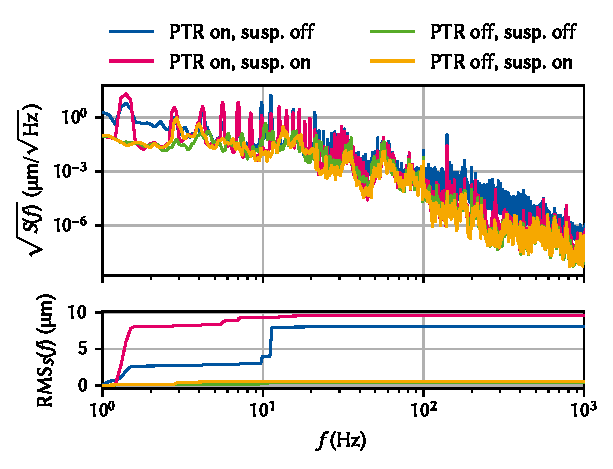
\includegraphics{img/pdf/setup/spect_accel}
    \caption[\imgsource{img/py/setup/vibration_spectroscopy.py}]{
        Top: displacement noise spectra acquired with the accelerometer at room temperature when the \gls{ptr} is switched on (blue, magenta) or off (green and orange), and when the air suspension is switched enabled (magenta, orange) or disabled (blue, green).
        Bottom: band-limited \gls{rms} computed from the \glspl{psd} in the upper panel (\cf \cref{eq:speck:psd:bandpower}).
        Turning on the \gls{ptr} increases the \gls{rms} noise amplitude by more than an order of magnitude over the entire frequency spectrum.
        The suspension slightly worsens the total noise because the low-frequency pulses excite the system close to the air springs' resonance frequency of \qty{2.5}{\hertz}.
    }
    \label{fig:setup:vibrations:accel}
\end{figure}

To assess the impact of the \gls{ptr} and the suspension, I measured the displacement noise \gls{psd} for each combination of the two being switched on and off.
The cryostat was closed, its vacuum chamber evacuated, and the magnet, a significant seismic mass, mounted as usual.
The measurements are shown in \cref{fig:setup:vibrations:accel} together with the band-limited \gls{rms} (\cf \cref{eq:speck:psd:bandpower}),
\begin{equation}\label{eq:setup:vibrations:rms}
    \rms_S(f) = \sqrt{\int_{f_\mr{min}}^{f}\dd{f^\prime}S(f^\prime)}
\end{equation}
with $S(f)$ the displacement noise \gls{psd}.
When the \gls{ptr} is switched off, the spectra with and without suspension are dominated by broadband vibration noise, although quite some structure around \qtylist{15;33;60}{\hertz} can be observed.\sidenote[][*-6]{
    Note the curious peaks slightly offset from the second and third harmonic of the \gls{ptr} frequency in the spectrum with suspension enabled and \gls{ptr} disabled.
    We may speculate that these are due to the \glspl{ptr} of other cryostats in other labs in the vicinity that are transmitted through the floor.
    Two were running two rooms over at the time the data was acquired.
}
When it is switched on, the \gls{ptr} pulses at \qty{1.4}{\hertz} and a large number of its higher harmonics visually dominate the spectra.
Clearly, the suspension has a larger impact in this case, matching qualitatively the behavior discussed in \cref{sec:setup:vibrations:isolation}.
At high frequencies, it manages to almost completely suppress the broadband excitation observed without the suspension.
At low frequencies, on the other hand, the \gls{ptr} harmonics are amplified to the degree that the band-limited \gls{rms} is dominated by their contribution.
Only at around \qty{10}{\hertz}, the attenuation starts to take effect.
The accelerometer noise floor can be seen to roughly fall off as $1/f^2$, compatible with white noise in the signal conditioning electronics.
Overall, the \gls{ptr} is found to raise the displacement noise \gls{rms} amplitude from \qty{0.5}{\micro\meter} to \qty{10}{\micro\meter} while the suspension, over the entire frequency range, has at best no positive influence.

This result is less than encouraging.
At that level of \gls{rms}-fluctuations, we would have a slim chance of resolving micrometer-scale features using the microscope.
But is the \emph{absolute} magnitude of displacement noise at the sample position really the correct measure for the microscope performance?
Indeed, if the sample oscillates in phase with the objective and ocular lenses as well as the \gls{smf}, we will still obtain a perfect imaging fidelity.
So actually only the \emph{relative} displacements of sample, lenses, and detection fiber affect the achievable resolution of the microscope.
To characterize these, I developed an optical \emph{in-situ} technique to measure the displacement noise based on knife-edge reflectance fluctuations that I will present in the following section.

\section{Optical vibration spectroscopy}\label{sec:setup:vibrations:optic}
The gate electrodes on our samples are fabricated using two separate lithography processes; first, the smallest structures are written using electron-beam lithography in two steps.
Then, larger structures on the order of \qty{1}{\micro\meter} and above are written using optical lithography.
In the region where the two overlap on the mesa to establish electrical contact, the highly reflective \ch{Ti/Au} optical gates have a width of \qty{14}{\micro\meter} and a height of \qty{160}{\nano\meter} and lie on top of the poorly reflecting \ch{GaAs} surface, resulting in a step-like reflectance profile.
Scanning perpendicularly across such a straight edge between a poorly and a highly reflecting material is known as a knife-edge measurement and is frequently used to measure the spatial extent of a laser spot~\cite{Arnaud1971,Skinner1972,Khosrofian1983}.
We can use the same setup to measure the displacement noise; instead of manually shifting our knife edge across the beam spot, though, we measure the reflectance fluctuations induced by the knife edge fluctuating relative to the spot due to external perturbations.

\begin{marginfigure}
    \centering
    \begin{tikzpicture}[
    round/.style={rounded corners=10pt},%
    font=\footnotesize,%
]

    % Mesa edge
    \draw[thick]
        (-2,0)
        -- ++(4.5,0)
    ;
    % Gate
    \path[draw=black, thick, fill=RWTHblack10, round]
        (-0.75,1)
        -- ++(0,-2.5)
        -- ++(1.5,0)
        -- ++(0,2.5)
    ;
    \path[draw=black, thick, dashed]
        (-0.75,1)
        -- ++(1.5,0)
    ;
    % Scan direction
    \draw[->, thick]
        (0.25,-0.75)
        -- ++(1,0) node[right] [align=center]{Scan \\ direction}
    ;
    % Laser spot
    \draw[dashed]
        (0.75,-0.75) circle (0.25)
    ;
    % Coordinate axes
    \draw[->]
        (1.75,0.3)
        -- ++(0.5,0) node[above] {$y$}
    ;
    \draw[->]
        (1.75,0.3)
        -- ++(0,0.5) node[right] {$z$}
    ;
    \draw
        (1.75,0.3) circle (0.1) node[left] {$x$}
    ;

    % Labels
    \node (mesa) at (-1.5,-0.25) {Mesa};
    \node (gate) at (0,0) [align=center]{Optical \\ gate};

\end{tikzpicture}
    \caption[\imgsource{img/tikz/setup/knife_edge.tex}]{
        Sketch of the region of the sample used for optical vibration spectroscopy.
        The coordinate system follows the magnet's; $z$ is parallel to gravity, and $x$ is perpendicular to the \gls{qw} plane.
        The optical gate extends further north as indicated by the dashed line.
    }
    \label{fig:setup:vibrations:knife_edge:sketch}
\end{marginfigure}

The scenario is sketched in \cref{fig:setup:vibrations:knife_edge:sketch} in the coordinate system defined by the magnet such that $z$ is along gravity's axis and $x$ is the out-of-plane axis.
Focusing the laser (indicated by a dashed circle) onto the edge of the optical gate, we can move the sample using the $y$-axis nanopositioner and observe a decrease in reflected intensity if the gate is moved away from the laser and an increase if it is moved towards the laser.
This gradient in reflected intensity can be inverted to obtain the vibration noise along $y$ by monitoring the intensity as a function of time.

Let us take a closer look at the reflected intensity when the laser spot has a finite overlap with the edge of the gate.
Under the simplifying assumption of a perfectly sharp drop-off and taking the reflectance of the Gold gate to be unity, we can write the reflectance as function of the coordinate perpendicular to the gate edge at $y=0$ as
\begin{equation}\label{eq:setup:reflectance_step}
    \reflectance(y) = \begin{dcases}
        1, & y \leq 0 \\
        \reflectance_0, & y > 0,
    \end{dcases}
\end{equation}
where $\reflectance_0$ is the reflectance of the bare \ch{GaAs} surface.
Assuming a perfect Gaussian (\gls{tem}$_{00}$ mode) beam characterized by its waist radius $w_0$ at which the intensity drops to $1/e^2$ of its maximum value, the laser intensity profile in 1D is given by
\begin{equation}\label{eq:setup:gaussian}
    I(y) = I_0\exp(-\frac{2y^2}{w_0^2}),
\end{equation}
where $I_0 = P_0/w_0$ with $P_0$ the total beam power.
The power reflected when the spot partially overlaps with the reflectance step can then be expressed as the convolution
\begin{equation}\label{eq:setup:knife_edge}
    P_{\mr{r}}(y) = \reflectance(y) \ast I(y) = \frac{I_0 w_0}{2}\sqrt{\frac{\pi}{2}}\left[ 1 - (1 - \reflectance_0)\erf\left(\frac{y\sqrt{2}}{w_0}\right) \right]
\end{equation}
in the $yz$ focal plane, where $\erf(y)$ is the error function.

\begin{marginfigure}
    \centering
    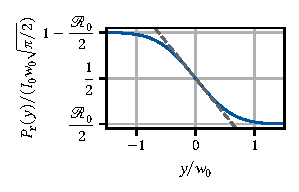
\includegraphics{img/pdf/setup/knife_edge_theory}
    \caption[\imgsource{img/py/setup/vibration_spectroscopy.py}]{
        Theoretical reflected power for a Gaussian beam of width $w_0$ and a reflectance contrast of $1-\reflectance_0$ according to \cref{eq:setup:knife_edge}.
        The dashed line indicates the leading order approximation at $y=0$.
    }
    \label{fig:setup:vibrations:knife_edge:theory}
\end{marginfigure}

The function $P_{\mr{r}}(y)$ is plotted in \Cref{fig:setup:vibrations:knife_edge:theory}.
The maximum contrast that can be achieved is given by $1-\reflectance_0$.
Furthermore, for $y\in[-w_0/2, w_0/2]$ the function is well-approximated by
\begin{equation}\label{eq:setup:knife_edge:approx}
    P_{\mr{r}}(y)\approx -I_0(1-\reflectance_0)y + \frac{I_0 w_0}{2}\sqrt{\frac{\pi}{2}}
\end{equation}
drawn as a dashed line.
Since we measure the photon count rate rather than the power, $\Phi = \flatfrac{P\lambda}{hc}$ with $\lambda$ the laser wavelength, we rewrite this as
\begin{equation}\label{eq:setup:knife_edge:linearized}
    \Phi_{\mr{r}}(y) = -sy + \frac{\Phi_0}{2}\sqrt{\frac{\pi}{2}}.
\end{equation}
where we defined the \emph{sensitivity}
\begin{equation}\label{eq:setup:knife_edge:sensitivity}
    s = \frac{\Phi_0}{w_0}(1 - \reflectance_0).
\end{equation}
Hence, to obtain a more sensitive probe for vibrations, meaning that small variations in $y$ lead to large variations in $\Phi_{\mr{r}}$, one could either improve the reflectance contrast $1-\reflectance_0$, decrease the spot size $w_0$, or increase the incident photon flux $\Phi_0$.\sidenote[][*-1]{
    Note that the smaller $w_0$, the smaller also the maximum displacement amplitude that can be resolved as the derivative goes to zero as $y\to\pm\infty$.
}
In our case, the former two are fixed by the sample and the setup, respectively , whereas the latter is limited by the maximum data transfer rate of the \tagger counting card, \qty{9}{\mega\sample\per\second}.

Starting from \cref{eq:setup:knife_edge:linearized}, it is straightforward to obtain the displacement in the vicinity of $y=0$ as function of photon flux,
\begin{equation}\label{eq:setup:knife_edge:procfn}
     y(\Phi_{\mr{r}}) = \frac{w_0}{1-\reflectance_0}\left[\frac{1}{2}\sqrt{\frac{\pi}{2}} - \frac{\Phi_{\mr{r}}}{\Phi_0}\right].
\end{equation}
To summarize, we can position the laser spot on the edge of an optical gate and record a time trace of the photon flux by using the \taggershort to count the photons detected by the \glspl{apd} mounted on the side exit of the spectrometer.
Using \cref{eq:setup:knife_edge:procfn} we can then convert the flux into a displacement and proceed with the usual spectral noise estimation as explained in \cref{part:speck}.

\begin{marginfigure}[*-13]
    \centering
    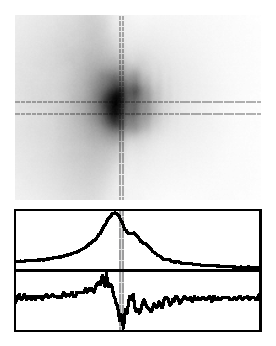
\includegraphics{img/pdf/setup/knife_edge}
    \caption[\imgsource{img/py/setup/vibration_spectroscopy.py}]{
        Calibration of the length reference scale.
        The top shows a \acrshort{cmos} camera image (higher intensity darker) of the white light spot on the edge of the optical gate as indicated in \cref{fig:setup:vibrations:knife_edge:sketch}.
        Several diffraction lines can be seen parallel to the edge.
        The vertical dashed lines indicate the region in which the intensity slope was fitted.
        The horizontal dashed lines indicate the extent of rows averaged over.
        The lower plots show a line cut along the central row of the considered region (top) and its derivative (bottom).
    }
    \label{fig:setup:vibrations:calibration:length_scale}
\end{marginfigure}

I will now lay out the experimental procedure of calibrating the system to (implicitly) obtain the parameters $w_0$, $\reflectance_0$, and $\Phi_0$.
The first challenge is obtaining a proper length reference scale.
While the nanopositioners on which the sample is mounted do in principle have a resistive position readout, it is extremely unreliable at small displacements.
Therefore, I calibrated the relative position using the imaging arm of the optical head.
\Cref{fig:setup:vibrations:calibration:length_scale} depicts the procedure.
Illuminating the sample with the white light, I positioned the spot on the edge of the optical gate and imaged the sample with the \cmoscam.
I then extracted the position of the edge, in pixels, for several rows to obtain some statistics by fitting a linear function to the edge profile in a small region between two refraction maxima.
Repeating this step for different DC voltages applied to the nanopositioner, this yields the proportionality factor between the nanopositioner DC voltage, $V_{\mr{DC}}$, and the position of the gate edge on the camera.
By measuring the total width of the gate on the camera image, I obtained the magnification by referencing it to the design width,
\begin{equation}\label{eq:setup:knife_edge:magnification}
    M = \frac{w[\unit{\pixel}]}{w[\unit{\micro\meter}]} = \frac{\qty{116}{\pixel}}{\qty{14}{\micro\meter}} \approx \qty{8.3}{\pixel\per\micro\meter}.
\end{equation}
Again performing a linear fit to the data for different voltages then results in the linear transformation from DC voltage to position (upper panel of \cref{fig:setup:vibrations:calibration:pos_vs_cps}).
Of course it is also possible to fit the full knife-edge function, \cref{eq:setup:knife_edge}, to the data shown in \cref{fig:setup:vibrations:calibration:pos_vs_cps}.
From this, the spot size $w_0$ and the actual bare \ch{GaAs} surface reflectance $\reflectance_0$ can be extracted.
Here we are content with the linear approximation; refer to \cref{subsec:app:setup:vibrations:knife_edge} for the full fits.

\begin{marginfigure}[*-15]
    \centering
    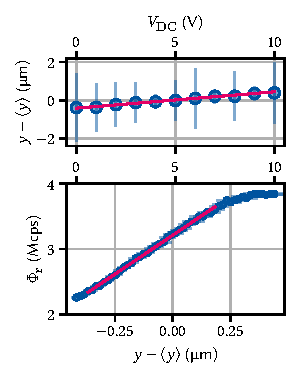
\includegraphics{img/pdf/setup/knife_edge_fits}
    \caption[\imgsource{img/py/setup/vibration_spectroscopy.py}]{
        Top: linear fit of the edge positions extracted from the analysis in \cref{fig:setup:vibrations:calibration:length_scale}.
        Error bars are propagated standard errors of the weighted average of edge positions extracted from different rows.
        Bottom: laser photon count rate as function of position set by the nanopositioner.
        Fitting the region $V_{\mr{DC}}\in[0.5, 7]\,\unit{\volt}$ yields $s\approx\qty{2.36+-0.02}{\mega\cps\per\micro\meter}$ (\cf \cref{eq:setup:knife_edge:linearized}).
        Error bars on $\Phi_{\mr{r}}$ show the standard error of the mean over multiple observations and error bars on $y$ show the fit error from the top panel.
    }
    \label{fig:setup:vibrations:calibration:pos_vs_cps}
\end{marginfigure}

Lastly, I switched from white light illumination to the laser, focused it onto the edge of a gate, and measured the photon count rate reflected off the sample as a function of $V_{\mr{DC}}$, from which we can finally extract the desired sensitivity (slope) $s\approx\qty{2.36+-0.02}{\mega\cps\per\micro\meter}$ of count rate over displacement.
The data and fit are shown in the bottom panel of \cref{fig:setup:vibrations:calibration:pos_vs_cps}.
Clearly, the count rate is linear in the displacement over a large range, indicating that for fluctuations with amplitude on the order of \qty{100}{\nano\meter} \gls{rms}, the measurement sensitivity should be sufficiently robust.

\begin{figure}
    \centering
    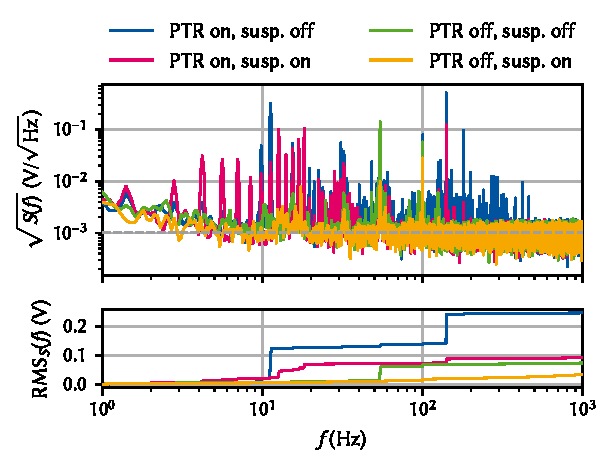
\includegraphics{img/pdf/setup/spect_optic}
    \caption[\imgsource{img/py/setup/vibration_spectroscopy.py}]{
        Top: displacement noise spectra acquired with the optical \emph{in-situ} method at room temperature when the \gls{ptr} is switched on (blue, magenta) or off (green and orange), and when the air suspension is switched enabled (magenta, orange) or disabled (blue, green).
        The dashed gray line indicates the theoretical noise floor derived in \cref{subsec:setup:vibrations:optic:noise_floor}.
        Bottom: band-limited \gls{rms} computed from the \glspl{psd} in the upper panel (\cf \cref{eq:speck:psd:bandpower}).
        The \gls{ptr} has a much smaller effect than when measuring the absolute displacement noise with the accelerometer, increasing the \gls{rms} only by a factor of two.
        While the lowest-order \gls{ptr} harmonics are amplified by up to an order of magnitude in amplitude with the suspension enabled, they contribute relatively little to the total \gls{rms} and are compensated by the superior high-frequency attenuation behavior.
        The total $\rms_S \approx \qty{100}{\nano\meter}$ with the cryostat in operation is below the typical \unit{\micro\meter} feature size.
    }
    \label{fig:setup:vibrations:optic}
\end{figure}

We are now at last able to measure the displacement noise using \pyspeck.
Setting \code{procfn} to the linear transformation given in \cref{eq:setup:knife_edge:procfn} and measuring the counts registered by the \glspl{apd} using the \taggershort,\sidenote{
    Since the \glspl{apd} are arranged in a \gls{hbt} geometry, I combined the counts of both instruments using the virtual channel functionality of the \taggershort.
}
I obtained the displacement noise \glspl{psd} shown in \cref{fig:setup:vibrations:optic}.
A few things stand out.
First, rather than the $f^{-2}$ background observed with the accelerometer in \cref{sec:setup:vibrations:accel}, the noise floor is white ($S(f)=\text{const.}$) at approximately $\qty{1}{\nano\meter\per\sqrt{\hertz}}$.
To understand why, we need to take a closer look at the counting statistics, which we will postpone for a bit in order to first finish our discussion of the noise spectra.
Second, the overall noise level is much -- by a factor of 20 \gls{rms} -- lower than with the accelerometer.
We can attribute this to the fact that the optical method is sensitive to relative rather than absolute displacements.
If the cryostat and the optical head were infinitely stiff we would measure no displacement noise with this method -- intrinsic noise floor notwithstanding -- whereas the accelerometer is still sensitive to oscillations of the cryostat on the air spring fulcrum.
In that sense the optical method gives us the more pertinent results because only the displacements seen by the light travelling through the microscope ultimately matter.
Third, in contrast to the accelerometer measurements, the \gls{rms} amplitude is reduced by half when the suspension is active.
Although the harmonics of the \gls{ptr} frequency of \qty{1.4}{\hertz} are again amplified by the suspension below \qty{10}{\hertz}, raising the band-limited \gls{rms} above that with the suspension disabled, there occurs a crossover at the eighth harmonic frequency beyond which the attenuation outweighs the amplification at low frequency.\sidenote{
    It furthermore appears that even a measurement whose sole electronic device is a picosecond-resolution counting card cannot escape \qty{50}{\hertz} power line noise (or in this case its second harmonic).
}

\subsection{Noise floor}\label{subsec:setup:vibrations:optic:noise_floor}
The noise floor in the optical vibration measurements shown in \cref{fig:setup:vibrations:optic} is qualitatively very different from that observed with the accelerometer.
There, the \emph{acceleration} noise floor was white,\sidenote{
    Remember that as acceleration is the second time derviative of displacement, in frequency space this translates to $y\propto a/f^2$ (\cref{eq:speck:fourier_derivative}).
}
whereas with the optical method the \emph{displacement} noise floor is white, hinting at a different underlying mechanism.

To elucidate this issue, and thereby understand the limitations of the optical vibration spectroscopy technique, we model the detection event of a single photon (a \enquote{click}) arriving at the detector at a random time $t_i$ as a $\delta$-function so that the total flux as function of time is given by
\begin{equation}\label{eq:setup:flux_comb}
    \Phi(t) = \sum_i \delta(t-t_i).
\end{equation}
Assuming them to be uncorrelated, the time difference between subsequent clicks is exponentially distributed with average rate $\bar{\Phi}$, $\lvert t_{i+1}-t_i\rvert\sim\expdist(\bar{\Phi})$~\cite{ExponentialDistributionWiki}.
From this it follows that the number of clicks $N(\dt)$ within a given time bin $t\in [s, u]$ of length $\dt = \lvert u - s\rvert$ is Poisson distributed, $N(\dt)\sim\poisson(\bar{N})$, with mean number of counts $\expval{N(\dt)} = \bar{N} = \bar{\Phi}\dt$~\cite{PoissonDistributionWiki}.
Using the formalism developed in \cref{sec:speck:theory:time_series_estimation}, we can now compute the \gls{psd} of the stochastic process $\delta N(\dt) = N(\dt) - \bar{N}$.
To this end, observe that because we assumed arrivals to be uncorrelated, $N_{u^\prime}(\dt)$ for a time bin starting at $t=u^\prime$ is independent of $N_{s^\prime}(\dt)$ for a time bin starting at $t=s^\prime$.
In other words, the autocorrelation function of $\delta N(\dt)$ is nonzero only for the same time bins,
\begin{equation}\label{eq:setup:poisson:autocorrelation}
    C_{\delta N(\dt)}(\tau) = \expval{(N_s(\dt) - \bar{N})(N_u(\dt) - \bar{N})} = \variance(N(\dt))\delta(\tau),
\end{equation}
where $\tau = s^\prime - u^\prime$ and $\delta(\tau)$ is to be understood in a broad sense as zero if $\abs{\tau} > \dt$ and $\flatfrac{1}{2\dt}$ else.
For the Poisson distribution the variance is equal to its mean so that we obtain
\begin{equation}\label{eq:setup:poisson:autocorrelation:evaluated}
    C_{\delta N(\dt)}(\tau) = \bar{N}\delta(\tau).
\end{equation}
In the limit of $\dt\to 0$, we can then perform the Fourier transform to obtain the \gls{psd} of $\delta N = \lim_{\dt\to 0}\delta N(\dt)$,\sidenote{
    Despite appearances, $S_{\delta N}$ has units \unit{\cts\squared\per\hertz}.
    The discrepancy stems from the difficulty in defining a continuous white noise process.
}
\begin{equation}\label{eq:setup:poisson:psd}
    S_{\delta N}(\omega) = \bar{N},
\end{equation}
that is, $\delta N$ is a white noise without frequency dependence.\sidenote{
    Note that we could have also arrived at this result directly by computing the autocorrelation function $\expval{\delta N(t)\delta N(t-\tau)}$ from \cref{eq:setup:flux_comb} with $N(t) = \int\dd{t}\Phi(t)$.
}
$S_{\delta N}$ can be seen as the \emph{instantaneous} number noise \gls{psd}.

As a last step, we consider once again discretely sampling the \emph{continuous} process $\delta N$ with \gls{psd} $S_{\delta N}(\omega)$ at rate $\fs=\dt\inverse$ in order to find an expression for the \gls{psd} of the discrete process $\delta N(\dt)$, $S_{\delta N(\dt)}(\omega)$.
We know from above that $\variance(\delta N(\dt)) = \bar{N}$.
On the other hand, recall from \cref{sec:speck:theory:time_series_estimation} that also
\begin{align}\label{eq:setup:shot_noise:var}
    \variance(\delta N(\dt)) = \intinf\ddf{\omega} S_{\delta N(\dt)}(\omega) = \int_{-\flatfrac{\fs}{2}}^{\flatfrac{\fs}{2}}\dd{f} S_{\delta N(\dt)}(f)
\end{align}
where the last equality holds true because of the finite bandwidth of the discretely sampled signal.
Since $S_{\delta N}$ is white, it follows that $S_{\delta N(\dt)}$ is, too, and we can directly evaluate \cref{eq:setup:shot_noise:var}, obtaining\sidenote{
    $S_{\delta N(\dt)}$ also has units \unit{\cts\squared\per\hertz}.
}
\begin{equation}\label{eq:setup:shot_noise:psd}
    S_{\delta N(\dt)}(\omega) = \frac{\bar{N}}{\fs}.
\end{equation}
To convert to the displacement noise \gls{psd}, we can simply convert units using the calibration derived above because if $N\sim\poisson(\bar{N})$ then so $y\sim\poisson(\flatfrac{\bar{N}\fs}{s})$ where $s$ is the slope of the calibration converting displacements to count rates, \ie, the sensitivity (see \cref{fig:setup:vibrations:calibration:pos_vs_cps,eq:setup:knife_edge:linearized}).
Hence,\sidenote{
    Note that this is the two-sided \gls{psd}; to convert to the one-sided version used in this chapter, multiply by two.
}
\begin{equation}\label{eq:setup:shot_noise:noise_floor}
   S_{\delta y(\dt)}(\omega) = \frac{\bar{N}}{\fs}\times\left(\frac{\fs}{s}\right)^2 = \frac{\bar{\Phi}}{s^2}
\end{equation}
with $\delta y = y - \expval{y}$.
This type of noise is known as \emph{shot noise}.
It was first studied in the context of electron transport by \citet{Schottky1918} and results from the discrete nature of, in our case, photons and their stochastic emission times~\cite{Blanter2000}.
For the parameters in the present measurements, $\bar{\Phi}\approx\qty{3}{\mega\cps}$ and $s\approx\qty{2.36}{\mega\cps\per\micro\meter}$ (\cf \cref{fig:setup:vibrations:calibration:pos_vs_cps}), we obtain a shot noise floor of $S_{\delta y(\dt)}\approx\qty{1}{\nano\meter\per\sqrt{\hertz}}$ in excellent agreement with the data shown in \cref{fig:setup:vibrations:optic} where the theoretical value is indicated by a gray dashed line.

Inserting the theoretical expectation for the sensitivity $s$, \cref{eq:setup:knife_edge:sensitivity}, into \cref{eq:setup:shot_noise:noise_floor}, we find that
\begin{equation}\label{eq:setup:shot_noise:noise_floor2}
    S_{\Delta y(\dt)}(\omega) = \frac{\epsilon}{\Phi_0}\left(\frac{w_0}{1-\reflectance_0}\right)^2
\end{equation}
if we identify $\bar{\Phi} = \epsilon\Phi_0$ for some (fixed) setup efficiency \eps.
This shows a clear path towards improving the \gls{snr} of the method.
Just as the sensitivity $s$ is improved by increasing $\bar{\Phi}$ and $1-\reflectance_0$ and by decreasing $w_0$, so is the shot noise floor, albeit quadratically in $w_0$ and $1-\reflectance_0$.
For example, for a reduction in spot size by a factor of two from inserting a different objective lens and a tenfold increase in maximum count rate achieved by replacing the counting card with a more powerful model,\sidenote{
    \swinst offers models with up to \qty{1.2}{\giga\sample\per\second}, although at that rate the jitter and dead time of the \glspl{apd} would start to become the limiting factors~\cite{SwabianTimeTagger}.
    Since very high frequencies are not of interest, a simpler photo-diode that supports batched measurement would also suffice.
}
our simple model predicts a noise floor of $\qty{25}{\pico\meter\per\sqrt{\hertz}}$, a reduction by a factor of \num{40}.

\begin{figure}
    \centering
    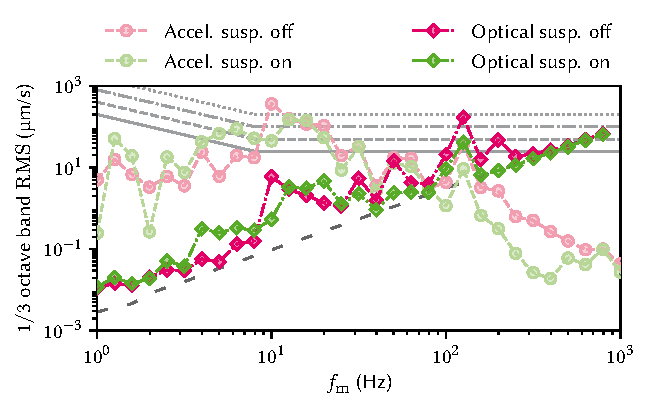
\includegraphics{img/pdf/setup/vc}
    \caption[\imgsource{img/pdf/setup/vibration_spectroscopy.py}]{
        $\flatfrac{1}{3}$ octave band \gls{rms} velocity computed for vibration measurements with the \gls{ptr} enabled and the suspension disabled (magenta) or enabled (green).
        Circles (diamonds) show data obtained with the accelerometer (optical method).
        The \glspl{vc} \acrshort{vc}-B, \acrshort{vc}-A and first two \acrshort{iso} levels are indicated as gray lines (solid, dashed, dash-dotted, dotted); see \cref{tab:setup:vibrations:vc}.
        Accelerometer data are above the \acrshort{vc}-B criterion for about three octaves centered around $f_{\mr{m}}=\qty{10}{\hertz}$, where even the \acrshort{iso} \enquote{residential day} level is breached.
        Optical data are more favorable, in particular with the suspension enabled (green).
        Towards high frequencies, the data are dominated by the wideband shot noise floor indicated by the loosely dashed dark gray line, suggesting the true displacement \gls{rms} is well below the \acrshort{vc}-B criterion.
    }
    \label{fig:setup:vibrations:vc}
\end{figure}

To conclude this section, let us come back to the \acrlongpl{vc} defined in \cref{subsec:setup:vibrations:isolation:theory} and evaluate the microscope based on the two different measurement methods presented in this chapter.
The $\flatfrac{1}{3}$ octave band \gls{rms} velocities computed for the vibration spectra with \gls{ptr} enabled shown in \cref{fig:setup:vibrations:accel,fig:setup:vibrations:optic} are plotted in \cref{fig:setup:vibrations:vc}.
Based on the data from the accelerometer (circles), the microscope does not meet the targeted level of vibration isolation (\acrshort{vc}-B, solid gray line) over three octaves.
Because this method of measuring the vibration noise is sensitive to absolute changes, we can understand qualitatively why this is the case if we view the accelerometer at the sample position as the end of a large pendulum whose fulcrum is in the center of the plane spanned by the three air springs.
A rough estimate gives a resonant frequency of \qty{0.5}{\hertz},\sidenote{
    The center of mass sits close to the magnet approximately $l = \qty{1}{\meter}$ below the springs so that we have $f = (2\pi)\inverse\sqrt{\flatfrac{g}{l}}\approx\qty{0.5}{\hertz}$.
}
implying frequencies in the considered range, $[4, 32]\,\unit{\hertz}$, are fairly effective at exciting motion in the pendulum (\cf \cref{subsec:setup:vibrations:isolation:theory}).
By contrast, with the optical method we do not pick up on such motion because the ocular lens focusing the light into the \gls{smf} is fixed in the co-rotating frame with respect to our imagined pendulum.
Indeed, the \gls{vc} velocities computed for this method show that they are orders of magnitude smaller at low frequencies in particular since only deviations from the rigid body picture established above induce a change in signal.
Furthermore, the \gls{rms} is dominated by the broadband shot noise floor indicated by the loosely dashed dark gray line, implying that the true vibration-induced \gls{rms} is well below our targeted \acrshort{vc}-B criterion.

\section{Routes for improvement}\label{sec:setup:vibrations:outlook}
Several improvements could be made to the system if the external conditions would allow it.
First, the rotary valve motor should be moved further away from the cold head.\sidenote{
    Clearly, this will impact the performance of the \gls{ptr} to some extent and should therefore be considered carefully.
}
As per the initial installation status, it is currently connected to the cold head with a flexible hose at a right angle and a distance of roughly \qty{50}{\cm}, which is below the minimum bend radius recommended by \oxinst.\sidenote{
    Note that the orientation of the motor, which is horizontal with the axis, is also not the recommended configuration.
}
Additionally, the term \enquote{flexible} is relative here given the pressure of \qty{20}{\bar}.
Increasing the length of the hose should reduce its relative rigidity and thereby its ability to transmit vibrations from the motor to the cold head.

Next, the cold head should be mounted firmly to a secondary reference frame, for instance the ceiling or the lower cryostat frame on which the springs rest.
An intuitively obvious step, it has also been shown in the literature that decoupling the \gls{ptr} from the cryostat in this fashion leads to significant improvements in vibration isolation~\cite{Olivieri2017}.\sidenote{
    The former option was attempted, but showed no clear improvements in the measurements for reasons unclear, see \cref{sec:app:setup:vibrations} for additional data.
    It did emphatically deteriorate the inter-departmental atmosphere.
    Apologies to the institute on the floor above.
}
Acoustic insulation of the room and \gls{ptr} flex hoses could further improve the low-frequency response of the system~\cite{Schmoranzer2019,Oh2021}.
Lastly, let me note that there also exist cryocoolers with variable operating frequency that can thus be tuned away from problematic resonances in the system~\cite{TransMitPTR}.

In \cref{sec:app:setup:vibrations} I show additional spectroscopy data, including data measured along the gravitational axis in the puck and on the floor of different rooms, which suggests moving to a different laboratory could also benefit the vibration stability, as well as data for different configurations of the \gls{ptr} motor.

% mainfile: ../../main.tex
\chapter{Conclusion \& outlook}\label{ch:setup:conclusion}
\AutoLettrine{Noise}

\begin{marginfigure}
    \centering
    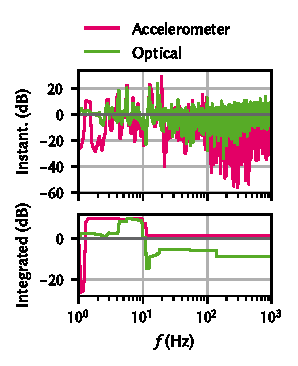
\includegraphics{img/pdf/setup/spect_dB}
    \caption[\imgsource{img/py/setup/vibration_spectroscopy.py}]{

    }
    \label{fig:}
\end{marginfigure}



\pagelayout{wide} % No margins
\part{Optical Measurements of Electrostatic Exciton Traps in Semiconductor Membranes}
\label{part:exp}
\pagelayout{margin} % Restore margins
\glsresetall

% mainfile: ../../main.tex
\chapter{Introduction}\label{ch:exp:introduction}
\begin{partcontribs}
    An overview of wafers measured in \thispart is given in \cref{tab:app:exp:samples}.
    Nikolai Spitzer\sidenote[a]{Ruhr-Universität Bochum.} grew wafer \textsc{\#15460 (\enquote{Honey})}.
    Julian Ritzmann\sidenotemark[a] grew wafer \textsc{\#15271 (\enquote{Fig})}.
    Chao Zhao\sidenote[b]{Then at Forschungzentrum Jülich.} grew wafer \textsc{\#M1\_05\_49}.
    Thomas Descamps fabricated the sample \textsc{Doped M1\_05\_49-2}.
    Sebastian Kindel fabricated the samples \textsc{Honey H13} and \textsc{Fig F10}.
\end{partcontribs}

\AutoLettrine{Just} as quantum computers are conceived as the quantum analogon of classical computers with bits and logic operations switched out by quantum counterparts, so can one devise \emph{networks} of such objects, where quantum information generated or processed at a quantum \emph{node} is distributed across long distances through the quantum counterparts of classical information channels~\cite{Nielsen2011,Simon2017}.
Famously envisioned by \citet{Kimble2008}, the concept can be extended to the idea of a \emph{quantum internet}.
A wide array of ideas has been put forth that make use of the theoretical capabilities of such quantum networks.

Initially, quantum networks were studied in the context of quantum cryptography~\cite{Bennett1984,Ekert1991,Deutsch1996,Gisin2002}.
There, the no-cloning theorem and clever use of entanglement ensure quantum-secured communication between distant parties that cannot be eavesdropped upon or tampered with by adversarial parties without detection.\sidenote{
    As ever in cryptography, new protocols keep getting hacked and loop-holes are discovered~\cite{Huang2018,Pang2020}.
    It will be interesting to see, therefore, if the security will faithfully transfer from theory to experiment.
}
Considerable attention has also been paid to the notion of distributed quantum computation~\cite{Cirac1999}.
As quantum computers do not appear to be on the same course of miniaturization as classical computers have been, there might turn out to be a limit to the physical size of quantum computers and, hence, a limit to the processing power of a monolithic node.
Distributed quantum computation resolves this bottleneck by allowing computations to be executed across separate nodes much like classical supercomputer clusters.
Although a comprehensive resource assessment of the feasibility of such approaches is still outstanding, initial results are promising~\cite{Jacinto2025}, and experimental demonstrations of small computations have recently been shown~\cite{Main2025}.
A concept combining distributed quantum computation with quantum cryptography is blind quantum computation~\cite{Childs2005,Giovannetti2013}, which promises a form of cloud-based quantum computation.
Also here first experimental demonstrations have been achieved~\cite{Wei2025}.

Next, quantum networks have garnered interest in the field of quantum sensing~\cite{Eldredge2018}.
This term refers to the branch of quantum technology in which individual quantum systems are employed as highly sensitive sensors, for example of magnetic fields, or, more generally, to perform measurements of physical quantities~\cite{Giovannetti2004,Degen2017}.
For example, there exist proposals to employ quantum networks for long-baseline telescopes that use optical interferometry to enhance the resolution of astronomical imaging~\cite{Gottesman2012,Khabiboulline2019}, akin to the techniques used to produce the first image of a supermassive black hole~\cite{TheEventHorizonTelescopeCollaboration2019}, or global networks of quantum clocks~\cite{Komar2014}.
Going beyond technological applications, the capability to coherently transmit quantum states across large distances opens the pathway to tests of quantum theory itself, and where it might fail~\cite{Weinberg1989}.\sidenote{
    This area of physics is termed \emph{foundations of physics}.
}
At least since the publication of the \gls{epr}--paradox~\cite{Einstein1935}, tests of the non-locality of quantum mechanics have been proposed~\cite{Bell1964,Clauser1969} and performed~\cite{Hensen2015,Storz2023}.
More recently, for example, a small quantum network was used to rule out a description of quantum theory by real numbers~\cite{Li2022} and we may expect more such experiments to come~\cite{Shadbolt2014}.
Indeed, as the first small-scale experimental demonstrators arrive~\cite{Knaut2024,Liu2024,Kucera2024,Stolk2024}, research into complex quantum networks and their properties and possible applications is still in its beginnings~\cite{Nokkala2024}.\sidenote{
    Take for example the recent interest in quantum causal order~\cite{Hardy2009,Goswami2020,Rozema2024}, originally envisioned to study gravitational effects on quantum coherence.
}

So how does such a quantum network work?
In the \enquote{canonical quantization} picture we already adopted previously, we might simply replace classical, optical links by quantum versions thereof and similarly transmit \emph{flying} qubits instead of bits through those channels.
However, even optical fibers, the backbone of the modern internet, are lossy, and since the photon loss scales exponentially with distance, there would be little hope to build networks larger than a few to a few tens of kilometers.\sidenote{
    We can expect a survival probability of \qty{1}{\percent} over a distance of \qty{100}{\kilo\meter}~\cite{Azuma2023}.
    There is therefore arguably no feasible alternative to optical transmission over long distances.
}
In classical networks, this problem is remedied by repeater stations that simply produce copies of incoming photons and thus amplify the signal.
In quantum mechanics, however, this is forbidden by the no-cloning theorem, which states that one cannot achieve a perfect copy of a qubit prepared in an arbitrary and unknown quantum state~\cite{Wootters1982,Dieks1982}.
To the rescue comes, then, entanglement.
By letting two adjacent repeater stations share a bipartite maximally entangled state (often referred to as a \gls{epr} or Bell pair), a station, Charlie, positioned between two others, Alice and Bob, each of whom Charlie shares Bell pairs with can perform a Bell measurement on the two halves of the pairs in his possession und thereby project Alice and Bob's halves into a state that is maximally entangled between the two of them.
This technique of entangling two states that have never interacted with each other is known as entanglement swapping~\cite{Zukowski1993,Pan1998}.
\citet{Briegel1998,Dur1999} then proposed a quantum repeater protocol that uses entanglement swapping, enhanced by entanglement distillation,\sidenote{
    Also known as entanglement purification.
}
to successively entangle neighboring pairs of entangled states whose resource requirements scale logarithmically with the length of the quantum channel between the ends of which entanglement needs to be established.
What is more, the protocol tolerates error and loss rates on the percent level and is thus much more benign than \gls{qec}.
Following the initial proposal, more improved schemes were developed that tolerate higher errors~\cite{Dur2007} or employ entirely different techniques~\cite{Bayrakci2022}, see \citer{Azuma2023} for a review, and recently also experimental realizations have been shown~\cite{Krutyanskiy2023}.

A crucial detail of the protocol is that it requires storing Bell states until the heralding of successful entanglement in a quantum memory.\sidenote{
    I note that there exist also protocols for memoryless, all-optical quantum repeaters~\cite{Li2019,Azuma2023}.
}
In practice, this means that quantum repeaters require a coherent light-matter interface between photonic flying qubits and stationary quantum memory since storing photons is not feasible.
Such an interface has been the subject of intense research and there exist a large number of competing approaches that differ in choice of material platform for the memory and choice of encoding for the photon~\cite{Awschalom2018,Beukers2024}.
Among the most advanced are atomic and defect-based systems.
Atomic (and ionic) systems are a natural choice as the energy scales of atomic transitions are compatible with photons in the telecom range ($\sim\qty{1550}{\nano\meter}$)~\cite{Sangouard2011,Covey2023,Krutyanskiy2023,Liu2024,Kucera2024}.
Nuclear spins coupled to defects in crystal lattices have long spin lifetimes at the same time as optical transitions~\cite{Togan2010,Nguyen2019,Bergeron2020,Stolk2024,Knaut2024}.
Optically interfacing semiconductor spin qubits\sidenote{
    By semiconductor spin qubits, I refer to qubits encoded in the spin of one or more electrons or holes confined in \glspl{qd}, in contrast to spins attached to charged defect centers or nuclear spins.
}
or superconducting qubits, on the other hand, is arguably more challenging because of a separation of energy scales.
While qubits in these systems have energy splittings in the \unit{\giga\hertz} regime, telecom photons have energies of hundreds of \unit{\tera\hertz}, and so bridging this gap requires some sort of intermediary or \emph{transducer}.
For superconducting qubits, approaches based on mechanical resonators~\cite{Mirhosseini2020} and electro-optic nonlinear materials~\cite{Wang2022} have been pursued among others.
For spin qubits, excitons (or complexes thereof) confined in \glspl{oaqd} such as self-assembled \glspl{qd}~\cite{Stranski1937,Koguchi1991,Koguchi1993,NobuyukiKoguchi1993} appear to be most promising owing to their excellent optical properties.
Due to the fast recombination speeds of excitons, their suitability as a qubit is limited.
Single charge carriers confined to \glspl{saqd} have been explored instead~\cite{Warburton2013}, but still face the problem that the growth of \glspl{saqd} is random and as such coupling two or more qubits is extremely challenging.
By contrast, spin qubits confined in \glspl{gdqd} have reached a high level of maturity~\cite{Burkard2023,Stano2025}, and the promise of scalability by leveraging the highly advanced industrial semiconductor fabrication technology still holds true.

\citet{Jocker2019} thus proposed a protocol for transferring the quantum state of a photonic, polarization-encoded qubit to that of a spin qubit confined in a \gls{gdqd} by means of a \gls{oaqd} serving as intermediary in order to benefit from the benign optical properties of the latter and the long coherence times and processing capabilities of the former.
In the protocol, an incident photon generates an exciton in the \gls{oaqd}, transferring the quantum state to the exciton.
By application of a strong in-plane magnetic field, bright and dark states of the exciton are mixed and electron and hole remain in a product state with all information encoded in the electron spin.
This allows discarding the hole and subsequently transferring the electron state to the \gls{gdqd}, the details of which depend on the encoding chosen, either single-spin (\gls{ld}) or two-spin (\gls{st}) qubit.
The protocol is agnostic to the precise realization of the \gls{oaqd}, although it adopts parameters from \glspl{saqd}.
A crucial ingredient of the protocol is that the \gls{oaqd} be in tunnel-coupling distance to the \gls{gdqd} in order to enable exchange coupling or the adiabatic transfer of the photo-electron.
For \glspl{saqd} this is a challenging endeavor since, as mentioned above, their growth is random and therefore requires one to first locate the dots and then align the gates during fabrication of the \gls{gdqd}.
Because of the exponential dependence of tunnel coupling on the distance, this alignment needs to be very precise indeed.

An alternative to an \gls{saqd} was proposed by \citet{Descamps2021} in form of an electrostatic exciton trap.
Here, excitons are designed to be confined not by local modifications of the band structure during growth but by application of out-of-plane electric fields through gate electrodes.
This tilts the band structure and lowers the exciton energy by the \gls{qcse}, where exciton dissociation is prevented by charge carrier confinement in a \gls{qw}.
To avoid dissociation by lateral electric fields, \citet{Descamps2021} developed a fabrication process to thin down the semiconductor heterostructure to a thin membrane symmetric about the \gls{qw}, allowing lithographic patterning of laterally aligned, nanometer-scale gate electrodes on both sides of the membrane~\cite{Descamps2023}.
Application of voltages of the same magnitude but opposite polarity to gates on the top and bottom side of the membrane then produces -- to leading order -- a local electric field without changing the chemical potential in the \gls{qw} itself, while voltages of the same polarity have just the opposite effect.
Together with the out-of-plane confinement by the \gls{qw}, this should in theory provide 0D-confinement of exciton purely by electrostatic means and allow for the top-down, scalable fabrication of \glspl{oaqd} in close proximity to other, conventional \glspl{gdqd}.
What is more, the confinement strength and potential relative to the neighboring \gls{gdqd} can be finely tuned by well-established techniques.

In \citer{Descamps2023}, \citeauthor{Descamps2023} demonstrated the implementation of the membrane fabrication process as well as initial progress towards forming a \gls{gdqd} in transport and optical measurement of the lowering of the local exciton potential by the \gls{qcse}.
Yet unobserved was the signature of \gls{qd}-behavior in an exciton trap as manifested by, for example, the resolution of orbital splittings or single-photon emission.
In \thispart, I present optical measurements of exciton traps towards this goal.
It is outlined as follows.
In \cref{ch:exp:theory}, I give an introduction to the physics of \gls{pl} in semiconductors as well as the influence of electric fields.
Following that, I introduce the \python measurement framework I wrote to control the experiment in \cref{ch:exp:mjolnir}.
Then, in \cref{ch:exp:observations}, I present measurements of doped membranes.
I show data of an exciton trap and discuss the voltage, power, and position dependence of the \gls{pl} emission as well as \gls{ple} measurements.
Finally, I perform simulations of the membrane structure to explain the quenching of \gls{pl} intensity observed when focusing a gate and propose slight modifications to the heterostructure design to mitigate this effect.
I conclude with an outlook in \cref{ch:exp:conclusion}.
% mainfile: ../../main.tex
\chapter{Photoluminescence and excitons in semiconductors}\label{ch:exp:theory}
\AutoLettrine{Semiconductors} are the foundation of the modern age of technology.
In large parts, this is due to their favorable optical properties, determined chiefly by their band gap on the order of \qty{1}{\electronvolt}, that enable wide-ranging applications from semiconductor lasers over photo-detectors to optical communication technology.
Semiconductors can be classified into \emph{direct} and \emph{indirect} categories, where the terminology refers to the location of the band gap, that is, the smallest energy difference between valence and conduction band in the Brillouin zone.
A direct semiconductor's band gap features a valence band maximum at the same point in $k$-space as a conduction band minimum.
Such materials, a prime example of which is the compound \ch{GaAs} with a band gap of $E_{\mr{g}}=\qty{1.519}{\electronvolt}$ at $T=\qty{0}{\kelvin}$ in the \gls{nir} spectrum~\cite{Vurgaftman2001}, emit electromagnetic radiation with energy $h\nu = E_{\mr{g}}$ when electrons excited from the valence into the conduction band recombine with a hole.
When the excitation occurs through optical absorption, this effect is known as \acrlong{pl}.

Of course, besides their optical applications, semiconductors are also the backbone of the modern electronics industry.
Their band gap allows tuning the conductivity by means of the field effect wherein the potential and thereby the band structure is locally modified by means of a voltage applied to a gate electrode.
This facilitates the construction of voltage-controlled transistors.
The development of remote-doping techniques then enabled the growth of extremely high-mobility \glspl{2deg} in \GaAsAlGaAs heterostructures~\cite{Ihn2009}.
In these structures, dopants are introduced into the \ch{AlGaAs} barrier layer some \qty{50}{\nano\meter} away from the \ch{GaAs} layer and thus spatially separated by a \ch{AlGaAs} spacer layer.
This reduces Coulomb scattering in the \gls{2deg} induced by the doping and produces very high-quality samples as evidenced for example by the observation of the fractional quantum Hall effect~\cite{Stormer1999a}.
It is hence not at all surprising that early quantum dot experiments also took place in this well-understood material system.
While undoped approaches to electron and hole spin qubits in \ch{GaAs} exist~\cite{Harrell1999,Chen2012,Li2014,Tracy2014}, they introduce added complications because of the need to electrostatically induce a \gls{2deg} and reliably contacting it~\cite{Rossler2016}.
What is more, these issues are exacerbated when the structures need to be thinned down to a membrane~\cite{Descamps2021,Kindel2025}.
Therefore, to accommodate \glspl{gdqd} next to the \gls{oaqd} in the membrane, the devices measured in \thispart are fabricated on doped heterostructures hosting a \gls{2deg}.
In the following, I discuss the optical behavior of these structures under illumination.\sidenote{
    The \emph{electrical} behavior is another matter; there, illumination can lead to the creation, trapping, and de-trapping of free charge carriers that alter the transport properties of the device, leading to electrical hysteresis and instability~\cite{Fujita2021,Shetty2022,Wang2023,Reznikov2024,Kindel2025}.
}
I take a simple analytical approach in order to capture the most relevant physics and obtain a qualitative understanding.
For quantitative results, a more detailed method incorporating electrostatics would be required; I refer the reader to \citer{Descamps2021} for such simulations.

\section{Photoluminescence in doped \GaAsAlGaAs heterostructures}\label{sec:exp:theory:pl}
Consider an intrinsic, direct-gap, Zincblende semiconductor such as \ch{GaAs} with a band gap of $E_{\mr{g}} = \qty{1.519}{\electronvolt}$ at zero temperature~\cite{Vurgaftman2001}.
At the $\Gamma$-point, the conduction band is well approximated by a parabolic band with effective mass $m^\ast_{\mr{c}}/m_{\mr{e}} = 0.067$ and is offset by $E_{\mr{g}}/2$ above the Fermi level $\mu$.
Offset by the same absolute amount in the opposite direction is the valence band, which close to $\Gamma$ is fourfold degenerate with heavy and light holes with effective masses $m^{\ast}_{\mr{hh}}/m_{\mr{e}} = 0.34$ and $m^{\ast}_{\mr{lh}}/m_{\mr{e}} = 0.09$, respectively~\cite{Miller1984a}.
The third valence band\sidenote{
    The valence bands are $p$-like and hence contain contributions from three twofold degenerate atomic orbitals.
}
is split off by the spin-orbit interaction and lies \qty{0.34}{\electronvolt} below the other valence bands~\cite{Davies2009}.
Introducing confinement in one direction, for example by doping a \GaAsAlGaAs heterojunction or growing a \ch{GaAs} \gls{qw} sandwiched between two layers of \ch{AlGaAs}, lifts the fourfold degeneracy of light and heavy holes and leaves -- under usual conditions -- the latter as the valence band ground state.

\begin{marginfigure}
    \centering
    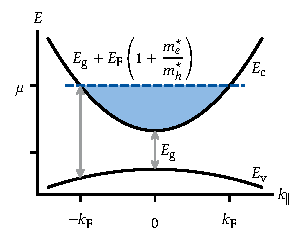
\includegraphics{img/pdf/experiment/2deg_sketch}
    \caption[\imgsource{img/py/experiment/pl.py}]{
        Band structure diagram of a doped heterostructure (after \citer{Kamburov2017}).
        Due to the $n$-type doping, the conduction band is filled up to the Fermi level $\mu$.
        Photonic excitation of an electron-hole pair can only occur at $\abs{k} > k_\mr{F}$ into the free states above $\mu$ due to the small photon momentum.
        Recombination can occur within a bandwidth of $E_\mr{F}(1 + m^\ast_{\mr{c}}/m^\ast_{\mr{hh}})$.
    }
    \label{fig:exp:theory:bandstructure:doped}
\end{marginfigure}

Doping in sufficiently high concentration then raises the Fermi level from mid-gap to inside the conduction band in the plane of confinement, resulting in a band structure as sketched in \cref{fig:exp:theory:bandstructure:doped}.
The bands remain parabolic as function of the in-plane wave vector $k_{\parallel}$ close to $\Gamma$.
The conduction band is filled up to $\mu$ where, measured from the conduction band edge, $E_{\mr{c}}(k_{\parallel} = k_{\mr{F}}) = E_{\mr{F}} = \hbar^2 k_{\mr{F}}^2/2m^\ast_{\mr{c}}$ with the Fermi wave vector $k_{\mr{F}}\sim\qty{1e8}{\per\meter}$.
Now, absorption of a photon incident on the semiconductor demands conservation of energy and momentum.
The latter condition implies that hole and electron have close to equal momentum because $k_{\gamma} = 2\pi/\lambda\approx\qty{8e6}{\per\meter}$ is much smaller than $k_{\mr{F}}$.
Thus, excitation of an electron-hole pair from the valence into the conduction band occurs only for $k\geq k_{\mr{F}}$.
By contrast, recombination can take place for any $k$ in principle.
In practice, however, photo-electrons quickly relax down to the Fermi level, and recombination takes place between electrons inside the Fermi sea and photo-holes somewhere in the valence band at $k\leq k_{\mr{F}}$.\sidenote{
    For sufficiently localized states in real space, a wide range of $k$ states in the valence band is available for recombination as states are extended in $k$-space.
    We can estimate the localization length required for states up to $k_{\mr{F}}$ to participate by $\Delta x \geq\flatfrac{1}{2\Delta k} = 1/2k_{\mr{F}}\sim\qty{5}{\nano\meter}$ for a typical \gls{2deg}.
}
The former condition then implies $E_{\gamma} \geq E_{\mr{g}} + E_{\mr{F}}\left(1 + m^{\ast}_{\mr{c}}/m^{\ast}_{\mr{hh}}\right)$ because no free electron states are available in the conduction band below $\mu$ due to the Pauli exclusion principle and where the term in parentheses is due to the valence band dispersion.
Many-body effects due to localized photo-holes scattering with electrons of the Fermi sea can lead to a strong enhancement of luminescence intensity at the Fermi edge, the so-called \gls{fes}~\cite{Mahan1967,Mahan1967a,Skolnick1987}.
The intensity of the \gls{pl} at the Fermi edge relative to recombination at the band edge ($k_{\parallel} = 0$) is thus an indicator of the \gls{qw} interface quality and degree of alloy fluctuations, both of which lead to hole localization~\cite{Melin2000,Gabbay2008}.

Free electron-hole pairs created by photo-excitation can form hydrogenic bound states due to the Coulomb attraction of their opposite electric charges, \emph{excitons}.
In two dimensions, this effect is strongly enhanced due to the increased overlap of electron and hole wave functions.
Furthermore, the reduced dimensionality also enhances the binding energy from $\sim\qty{4}{\milli\electronvolt}$ in bulk \ch{GaAs} to up to four times that in \ch{GaAs} \glspl{qw}~\cite{Andreani1990,Gilliland1997}.
Rather than the continuum of the joint density of states of valence and conduction band discussed previously, excitons are discrete states whose energy is lower than the band gap energy by the binding energy, $E_X = E_{\mr{g}} - E_{\mr{b}}$.
In doped \glspl{qw} hosting a \gls{2deg}, the free carriers can screen the exciton binding energy and lead to an ionized electron-hole plasma~\cite{Palmieri2020}.
This is known as the insulator-to-metal (Mott) transition in semiconductors~\cite{Mott1968}.
Competing with this are so-called Mahan excitons~\cite{Mahan1967,Mahan1967a} that give rise to the \gls{fes}~\cite{Schleife2011}.

Next, I discuss the influence of an electric field on excitons.
For this, we return to undoped structures for simplicity.

\section{The quantum-confined Stark effect}\label{sec:exp:theory:qcse}
\begin{marginfigure}
    \centering
    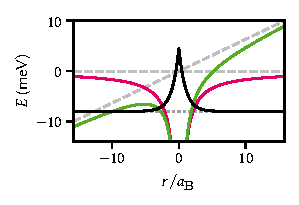
\includegraphics{img/pdf/experiment/in_plane_field}
    \caption[\imgsource{img/py/experiment/qcse.py}]{
        Effect of an in-plane electric field on an exciton wave function.
        In the hole's reference frame, the electron sees a static attractive Coulomb potential (magenta), resulting in a bound state (dotted gray line, wave function sketched in black).
        Applying an electric field ($F=\qty{100}{\milli\volt\per\micro\meter}$, dashed gray lines) tilts the Coulomb potential (green) and leads to a transparent barrier through which the electron can tunnel out.
    % In-plane fields -> field ionization -> line broadening \cite{Miller1985}
    }
    \label{fig:exp:theory:in_plane_field}
\end{marginfigure}

Consider the electron-hole pair in bulk \ch{GaAs} in the co-moving frame of the hole.
The hole generates the Coulomb potential
\begin{equation}
    V(r) = \frac{e}{4\pi\eps_0\eps_{\mr{r}}\abs{r}},
\end{equation}
where $\eps_{\mr{r}} = \num{13.3}$ is the relative permittivity of \ch{GaAs} at low temperatures, which attracts the electron by the Coulomb energy $E(r) = qV(r) = -eV(r)$.
\Cref{fig:exp:theory:in_plane_field} depicts the Coulomb potential in magenta and the bound electron's wave function sketched in black.
The electron-hole separation $r$ is shown in units of the exciton Bohr radius in two dimensions~\cite{Olsen2016}
\begin{equation}
    a_{\mr{B}} = \frac{2\pi\eps_0\eps_{\mr{r}}\hbar^2}{\mu e^2} = \qty{6}{\nano\meter}
\end{equation}
with $\mu$ the reduced effective mass of conduction and heavy-hole valence bands.

We now apply an electric field $F$.
This modifies the potential seen by the electron by $erF$ as sketched in green \cref{fig:exp:theory:in_plane_field}.
Ignoring changes to the electron wave function, we can see that the electron can tunnel out of the Coulomb potential, leading to \emph{field-induced ionization} of the exciton.
Now place the exciton in a \gls{qw} instead of in bulk with the electric field pointed such that it is out-of-plane of the \gls{qw}.
The field still tilts the potential, but because electrons and holes are confined into a quasi-two-dimensional plane, they cannot escape and hence do not dissociate.
This is the \gls{qcse}~\cite{Miller1984}.

In order to obtain a qualitative understanding of the \gls{qcse}, consider an undoped \ch{GaAs/Al_{0.33}Ga_{0.66}As} \gls{qw} of width $L = \qty{20}{\nano\meter}$.
We take a 57:43 ratio for the band offsets~\cite{Miller1984a}, resulting in discontinuities of height $\Delta E_{\mr{c}} = \qty{0.24}{\electronvolt}$ and $\Delta E_{\mr{hh}} = \qty{0.18}{\electronvolt}$ at the interfaces for the conduction and the heavy-hole valence band, respectively, and $m^\ast_{\mr{c}}/m_{\mr{e}} = \num{0.067}$ and $m^\ast_{\mr{hh}}/m_{\mr{e}} = \num{0.34}$ for the effective masses.\sidenote{
    I note that the literature knows many different values for the hole effective mass in the plane of a quantum well, suggesting that one should actually measure it to be confident in the actual value.
}
Assuming an infinitely deep well for simplicity, the eigenenergies are
\begin{equation}\label{eq:exp:theory:square_well:eps}
    E_n = \frac{1}{2 m^\ast}\left[\frac{\pi\hbar n}{L}\right]^2
\end{equation}
and the eigenstates are
\begin{equation}\label{eq:exp:theory:square_well:psi}
    \psi_n(z) = \sqrt{\frac{2}{L}}\sin(\frac{n\pi z}{L}).
\end{equation}
The ground state energy is then \qty{14}{\milli\electronvolt} (\qty{3}{\milli\electronvolt}) above (below) the conduction (valence) band edge, corresponding to \qty{6}{\percent} (\qty{2}{\percent}) of the respective band offsets and implying that the infinite-well approximation is acceptable,\sidenote{
    In a finite well, the wave functions decay exponentially into the barriers and result in slightly lower eigenenergies.
    However, the qualitative behavior remains the same.
}
while the first excited state lies \qty{42}{\milli\electronvolt} higher than the ground state.
The upper panel of \cref{fig:exp:theory:qcse:bandstructure} depicts the first two wave functions of electrons and holes in a band structure diagram.
Due to the symmetry of the confining potential, the wave functions are symmetric around the center of the well.

Now, applying an out-of-plane electric field tilts the bands and pulls electrons and holes to opposite interfaces of the \gls{qw}.
The Hamiltonian for the electrons in this case reads~\cite{Rabinovitch1971,Miller1985,Davies2009}
\begin{equation}\label{eq:exp:theory:qcse:hamiltonian}
    H = -\frac{\hbar^2}{2m^\ast}\dv[2]{z} + eFz
\end{equation}
if we take $z$ to be zero at an interface and choose $F \geq 0$.
Introducing the length and energy scales~\cite{Davies2009}
\begin{gather}
    \tilde{\eps} = \left[\frac{\left(\hbar eF\right)^2}{2m^\ast}\right]^{\frac{1}{3}}, \\
    \tilde{z} = \left[\frac{\hbar^2}{2m^\ast eF}\right]^{\frac{1}{3}} = \frac{\tilde{\eps}}{eF},
\end{gather}
and defining
\begin{equation}
    Z_n(z) = z/\tilde{z} - \eps_n/\tilde{\eps}
\end{equation}
with $\eps_n$ the eigenvalues of $H$, the Schrödinger equation becomes~\cite{Rabinovitch1971}
\begin{equation}\label{eq:exp:theory:qcse:se}
    \dv[2]{Z_n}\psi_n(Z_n) = Z_n\psi_n(Z_n).
\end{equation}
\Cref{eq:exp:theory:qcse:se} is known as the Stokes or Airy equation and has the general solution
\begin{equation}
    \psi_n(Z_n) = \alpha_n\Ai(Z_n) + \beta_n\Bi(Z_n),
\end{equation}
where $\Ai(z)$ and $\Bi(z)$ are the Airy functions.
$\Ai(z)$ and $\Bi(z)$ oscillate for $z < 0$ and decay (grow) exponentially for $z > 0$, respectively.
As we assumed infinitely high barriers at $z = 0$ and $z = L$, the boundary conditions impose
\begin{equation}
    \psi_n(Z_n(0)) = \psi_n(Z_n(L)) = 0,
\end{equation}
which completely determines the eigenstates and -energies.
For large well widths or fields ($eFL/\eps_n\gg 1$), the second term is exponentially suppressed and the eigenenergies are given by the zeros of $\Ai(Z_n)$.
For zero field, one recovers the square well solution (\cref{eq:exp:theory:square_well:psi,eq:exp:theory:square_well:eps}).

\begin{marginfigure}[*-34]
    \centering
    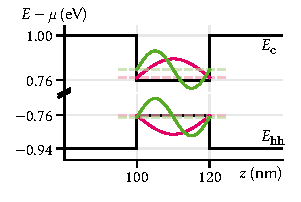
\includegraphics{img/pdf/experiment/qw_undoped_0V}
    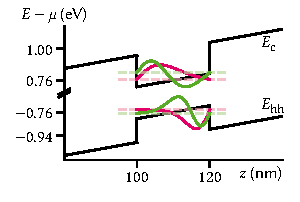
\includegraphics{img/pdf/experiment/qw_undoped_1V}
    \caption[\imgsource{img/py/experiment/qcse.py}]{
        \Gls{qcse} in an undoped \acrshort{qw}.
        Top: conduction and heavy-hole valence band profiles along the growth direction.
        The wave functions of the first two eigenstates in the well are drawn in magenta and green, respectively.
        The ground state transition is larger by $\Delta E = \qty{17}{\milli\electronvolt}$ than the gap $E_{\mr{g}}$ due to the confinement.
        Bottom: same structure as above with an out-of-plane electric field applied across the structure ($F=\qty{5}{\volt\per\micro\meter}$).
        Analytical wave functions in the infinite-well approximation are shown in magenta and green again.
        The wave functions get pushed to opposite interfaces of the \acrshort{qw}, lowering the ground state transition energy by $\Delta E = -\qty{10}{\milli\electronvolt}$.
        Excitonic effects are not included.
    }
    \label{fig:exp:theory:qcse:bandstructure}
\end{marginfigure}

The finite-field case is shown in the lower panel of \cref{fig:exp:theory:qcse:bandstructure} for $F=\qty{5}{\volt\per\micro\meter}$.
Owing to the larger effective mass of the heavy holes, the characteristic length scale $\tilde{z}$ is shorter and hence the corresponding wave functions are narrower (more localized) than their electronic counterparts.
The ground state transition energy at this field is \qty{10}{\milli\electronvolt} below the gap or \qty{27}{\milli\electronvolt} lower than in the zero-field case.

For a full quantitative accounting of the transition energies, the exciton binding energy as well as finite barrier heights would need to be included.
The former is on the order of \qtyrange{6}{9}{\milli\electronvolt} in \ch{GaAs} and becomes smaller as the overlap of the electron and hole wave functions is reduced when applying an electric field, pulling the wave functions to opposite interfaces~\cite{Miller1984}.
For the latter, \citet{Miller1985} found that finite-well properties could be reproduced by using effective well widths with infinite-well models.

\subsection{In-plane confinement}\label{subsec:exp:theory:qcse:trap}
% TODO: Motivate why we do all this! -> oscillator strength
So far, we have considered the \gls{qcse} in a single dimension, as if we were to apply a global electric field.
However, as we saw before, the field lowers the exciton energy below the \gls{qw} confinement and hence, if applied locally, results in an effective confinement potential in the plane of the \gls{qw}.
\citet{Descamps2021} performed numerical simulations for a geometry with circular gate electrodes with \qty{200}{\nano\meter} diameter on both sides of a membrane, finding a confinement depth of $V_0 =\qty{20}{\milli\electronvolt}$ at $F=\qty{5}{\volt\per\micro\meter}$ that is well approximated by a single-particle harmonic potential for the center-of-mass wave function of the exciton, $V(\rho) = M\omega^{2}\rho^{2}/2 - V_0$, with mass $M = m^\ast_{\mr{c}} + m^\ast_{\mr{hh}}$ and confinement strength $\omega/2\pi = \qty{738}{\giga\hertz}$ corresponding to an oscillator length $\xi=\sqrt{\hbar/M\omega}=\qty{20}{\nano\meter}$.
To obtain a qualitative picture, let us interpolate this result for different fields.
The depth of confinement corresponds to the energy shift induced by the \gls{qcse} and is quadratic in $F$, $V_0 = -\alpha F^2$.
At vanishing field, there should be no in-plane potential, $\omega=0$.
Hence, we can assume that $\omega\propto F$ to leading order and thus $V(\rho) = \beta M F^{2} \rho^{2}/2 - \alpha F^{2}$.

How does this in-plane confinement modify the wave function?
We ignore the relative motion of electron and hole as the optical properties of the exciton are dominated by the behavior at zero separation for $a_{\mr{B}}/\xi < 1$~\cite{Kavokin1994}, and consider only $\Delta n = 0$ transitions, \ie, electron and hole in the same $z$ quantum state, as $\Delta n\neq 0$ transitions are much weaker~\cite{Davies2009}.
Let us further initially assume a separable wave function and choose cylindrical coordinates according to the symmetry of the potential.
We then have
\begin{equation}\label{eq:exp:theory:qcse:trap:psi}
    \Psi_{np\ell}(z_{\mr{e}}, z_{\mr{h}}, \rho, \phi) = \psi_n(z_{\mr{e}})\psi_n(z_{\mr{h}})\chi_{p\ell}(\rho)\exp(i\ell\phi)
\end{equation}
where\sidenote{
    Note that \citet{Karimi2014} miss a factor $2\pi$ in the normalization.
}~\cite{Karimi2014}
\begin{equation}\label{eq:exp:theory:qcse:trap:ho:psi}
    \chi_{p\ell}(\tilde{\rho}, \phi) = \sqrt{\frac{2p!}{2\pi\xi^2(p + \abs{\ell})!}}\exp(-\tilde{\rho}^2/2)\tilde{\rho}^{\abs{\ell}}L_p^{\abs{\ell}}\left(\tilde{\rho}\right)
\end{equation}
with the associated Laguerre polynomial $L_p^{\abs{\ell}}(x)$ and we used the shorthand $\tilde{\rho} = \rho/\xi$.
The numbers $p\in\mathbb{N}$ and $\ell\in\mathbb{Z}$ denote the principal and orbital momentum quantum numbers.
The eigenenergies of the harmonic oscillator solution, \cref{eq:exp:theory:qcse:trap:ho:psi}, are given by
\begin{equation}\label{eq:exp:theory:qcse:trap:ho:eps}
    \eps_{p\ell} = \hbar\omega\left(2p + \abs{\ell} + 1\right).
\end{equation}
To account for a finite well width ($L\approx\xi$ in our case), we can to a first approximation perform the replacement $\rho\to r = \sqrt{\rho^2 + z^2}$ in \cref{eq:exp:theory:qcse:trap:psi}.
The resulting wave function $\Psi_{np\ell}(r, z_{\mr{h}})$ at fixed electron coordinate $z_{\mr{e}}$ is shown in \cref{fig:exp:theory:qcse:wf} for $n = \ell = 0$ (which makes it independent of $\phi$).
For $\ell=0$, $\Psi_{np\ell}$ has $n$ nodes along $z$ and $p$ nodes along $\rho$.

\begin{figure}
    \centering
    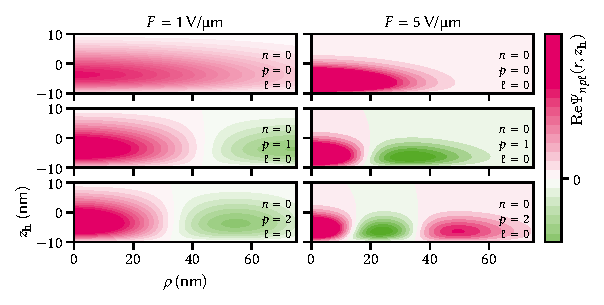
\includegraphics{img/pdf/experiment/wavefunction}
    \caption[\imgsource{img/py/experiment/qcse.py}]{
        Center-of-mass exciton wave function (hole sector) in a harmonic trap under an electric field.
        Left column shows the low-field and right column the high-field case.
        Top row is the ground state, middle and bottom row the first and second excited state in the plane, respectively.
        The out-of-plane wave function is the ground state in all cases ($n=0$) and the trap confinement strength $\omega/2\pi = \qty{738}{\giga\hertz}$ for $F=\qty{5}{\volt\per\micro\meter}$~\cite[Section~2.2.2]{Descamps2021} and linearly interpolated for \qty{1}{\volt\per\micro\meter} (see text).
    }
    \label{fig:exp:theory:qcse:wf}
\end{figure}

At last, we can use the exciton wave function $\Psi_{nm\ell}(r, \phi, z_{\mr{e}}, z_{\mr{h}})$ to estimate the \emph{oscillator strength}, a quantity often quoted in semiconductor spectroscopy.
The oscillator strength puts in relation the quantum mechanical transition rate with the emission rate of a classical oscillator with frequency $\omega = \Delta E/\hbar$ matching the transition energy~\cite{Hilborn1982}.
For a dipole transition from state $\ket{i}$ to state $\ket{j}$, it may be written as~\cite{Davies2009}
\begin{equation}
    f_{ji} = \frac{2\mu\Delta E_{ji}}{\hbar^2} \abs{\!\matrixelement{j}{\bvec{r}}{i}}^2,
\end{equation}
where $\mu$ is the reduced mass of the exciton.
As the selection rules only allow in-plane dipole transitions for heavy holes, we write~\cite{Kavokin1994}
\begin{subequations}\label{eq:exp:oscillator_strength}
    \begin{equation}\tag{\ref{eq:exp:oscillator_strength}}
        f_{np\ell} = \frac{2\mu\eps_{np\ell}}{\hbar^2} J_{r}^2 J_{\phi}^2 \abs{\!\matrixelement*{u_{\mr{c}}}{x}{u_{\mr{hh}}}}^2
    \end{equation}
    for transitions with $\Delta n = \Delta p = \Delta\ell = 0$, where
    \begin{align}
        J_{r} &= \int_{0}^{L}\dd{z}\int_0^{\infty}\dd{\rho}\rho\psi_n\gth{\mr{e}}(z)\psi_n\gth{\mr{h}}(z)\chi_{p\ell}(\sqrt{\rho^2 + z^2}), \label{eq:exp:theory:osc:rz} \\
        J_{\phi} &= \int_0^{2\pi}\dd{\phi}\exp(\i\ell\phi), \label{eq:exp:theory:osc:phi} \\
        \eps_{np\ell} &= \eps_n + \eps_{p\ell},
    \end{align}
\end{subequations}
and $\ket*{u_{\mr{c}(\mr{hh})}}$ are the Bloch functions of the valence and conduction band, respectively, that we have neglected so far.
From \cref{eq:exp:theory:osc:phi}, we immediately see that the oscillator strength of states with nonzero orbital momentum ($\ell\neq 0$) vanishes, $f_{np0}=0$!
This in turn implies from \cref{eq:exp:theory:qcse:trap:ho:eps} that the exciton level spacing in a radially symmetric trap is given by $\Delta E = 2\hbar\omega=\qty{1}{\milli\electronvolt}$, a factor of two larger than assumed by \citet{Descamps2021}.

As we tilt the bands, energy levels below the \gls{qw} become available in the barrier once $\Delta E_{\mr{c}(\mr{hh})} - \eps_{n} < eFd$ with $d$ the width of the barrier and $\Delta E_{\mr{c}(\mr{hh})}$ is the height of the conduction (valence) band discontinuity.
This allows confined carriers to escape the \gls{qw} with a finite probability by tunneling through the barrier, an effect known as Fowler-Nordheim tunneling.
If this probability becomes too large, trapped excitons can dissociate by electron or hole tunneling through the barriers before recombining, and thereby lower the radiative recombination efficiency (internal quantum efficiency, see \cref{subsec:setup:optics:coupling:efficiency}) and introduce additional errors in the spin-photon interface.
Following \citer{Davies2009}, we can estimate the tunneling probability as\sidenote{
    The same result up to a slightly different numerical prefactor in the exponent is obtained more formally from the WKB approximation~\cite{Descamps2021}.
}
\begin{equation}\label{eq:exp:theory:qcse:tunneling:probability}
    \mathscr{T}_n(F) \approx \exp\left\lbrace -\frac{\sqrt{4 m^\ast [\Delta E_{\mr{c}(\mr{hh})} - \eps_n]^3}}{e F\hbar}\right\rbrace.
\end{equation}
The tunneling rate $\Gamma_n$ can then be estimated by the frequency that a confined charge carrier \enquote{visits} the edge of the \gls{qw} multiplied by the probability that it tunnels, $\mathscr{T}_n$~\cite{Larsson1988}.
That is, we take $\eps_n$ to be a kinetic energy and calculate the velocity as
\begin{equation}
    v_n = \frac{\hbar k_n}{m^\ast_{\mr{c}(\mr{hh})}} = \sqrt{\frac{2 \eps_n}{m^\ast_{\mr{c}(\mr{hh})}}}.
\end{equation}
Then the frequency of one round trip inside the \gls{qw} is
\begin{equation}
    \tau_n\inverse = \frac{v_n}{2L} = \frac{1}{L}\sqrt{\frac{\eps_n}{2 m^\ast_{\mr{c}(\mr{hh})}}}
\end{equation}
and
\begin{equation}\label{eq:exp:theory:qcse:tunneling:rate}
    \Gamma_n = \frac{\mathscr{T}_n}{\tau_n}.
\end{equation}
What is the order of magnitude of $\tau_n$?
For an energy of $\eps_n = \qty{10}{\milli\electronvolt}$, $\tau_n\approx\qty{200}{\femto\second}$ for electrons and \qty{400}{\femto\second} for holes.
The tunneling probability $\mathscr{T}_n$ therefore needs to be quite small indeed for the rate $\Gamma_n$ to remain small.

\begin{marginfigure}
    \centering
    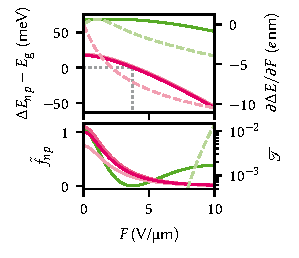
\includegraphics{img/pdf/experiment/qcse_field_dependence}
    \caption[\imgsource{img/py/experiment/qcse.py}]{
        Electric field dependence of the \gls{qcse} for the first two energy levels in the \gls{qw}.
        Top: the ground state energy (magenta) shows the expected quadratic dependence; the confinement energy is compensated at around $F=\qty{3.7}{\volt\per\micro\meter}$.
        Higher in-plane orbital levels are shown for the \gls{qw} ground state in decreasing saturation.
        For zero field, the splitting is zero as there is no in-plane confinement.
        At maximum field, the splitting is $2\hbar\omega = \qty{2}{\milli\electronvolt}$.
        Dashed lines (right axis) show the derivative, revealing that the \gls{qw} excited state is actually raised in energy at low fields.
        Bottom: oscillator strengths (same color code as above).
        Dashed lines (right axis) show the electron tunneling rate through the barrier, dash-dotted the holes.
    }
    \label{fig:exp:theory:qcse:field}
\end{marginfigure}

\Cref{fig:exp:theory:qcse:field} summarizes the \gls{qcse} in a \gls{qw} additionally confined in the plane by local electric fields.
The top panel shows the exciton transition energy $\Delta E_{np}$ for $\Delta n = \Delta p = 0$ in solid lines.\sidenote{
    Note again that we neglected the exciton binding energy, which decreases with increasing field and hence slightly reduces the redshift~\cite{Miller1984}.
}
The first three in-plane sublevels due to the harmonic potential are drawn in less saturated colors but hard to see because the level spacing is much smaller than the out-of-plane \gls{qw} subband spacing, $\sim\qty{1}{\milli\electronvolt}/\qty{50}{\milli\electronvolt}$.
The ground state shows the expected quadratic dependence on the electric field also obtained, for example, from perturbation theory.
Drawn as a dashed line is the induced dipole moment,
\begin{equation}
    \bvec{p}_{np}(F) = \pdv{\Delta E_{np}}{F}\ubvec{z},
\end{equation}
which is monotonously decreasing for the ground state as function of electric field $F$, consistent with a continuous lowering of energy.
For the first excited state, the induced dipole moment is actually positive below \qty{2}{\volt\per\micro\meter}, leading to a repulsive interaction and hence a raising of the transition energy by up to \qty{1}{\milli\electronvolt}.
The lower panel shows the oscillator strength, \cref{eq:exp:oscillator_strength}, normalized to its value of the ground state at zero field, $f_{00}(F=0)$.
For the ground state it decays exponentially with the electric field as the overlap between electron and hole wave functions, which decay exponentially into the \gls{qw} themselves, is reduced.
$f_{0p}$ for higher in-plane orbital states ($p > 0$, magenta, decreasing saturation) has an envelope following the ground state's exponential decay but vanishes at $p$ points in $F$ due to the fact that the wave function has $p$ nodes.
By contrast, $f_{10}$ for the first excited \gls{qw} state (green) does not decay to zero at large fields but also has a zero at an intermediate field because of the wave function's node along $z$.

Finally, the right axis shows the estimated tunneling rates (\cref{eq:exp:theory:qcse:tunneling:rate}) of the electron (hole) ground (excited) states in dashed (dash-dotted) magenta (green) lines, respectively.
Rates of electrons are at least four orders of magnitude larger than those of holes owing to their smaller effective mass despite the larger band offset.
At $F=\qty{5}{\volt\per\micro\meter}$ corresponding to a voltage of \qty{1}{\volt} across a membrane of \qty{200}{\nano\meter} thickness, the electron tunnel rate is on the order of \qty{1}{\hertz}, but rises very quickly above that.
Considering once again a \gls{qw} hosting a \gls{2deg} and neglecting associated band bending effects, the rate corresponds to a current through a circular area of \qty{1}{\micro\meter} in diameter of \qty{1}{\femto\ampere} at an electron density of $n = \qty{5e11}{\per\centi\meter\squared}$, but already \qty{500}{\pico\ampere} (\qty{800}{\kilo\hertz}) at \qty{7.5}{\volt\per\micro\meter}.
For single excitons, however, which have a lifetime on the order of \qty{1}{\nano\second}, even a tunnel rate of \qty{1}{\mega\hertz} results in a sufficiently low tunnel probability $\sim\qty{1}{\permill}$.

\section{Excitonic complexes}\label{sec:exp:theory:complexes}
If we liken the exciton to a Hydrogen atom\sidenote{Although positronium is a better analogon.} with modified binding energy $E_{\mr{b}}$ and Bohr radius $a_{\mr{B}}$, it is natural to expect molecules and ions of these states to exist.
The simplest molecule, or excitonic complex, is the biexciton, the analog of the \ch{H2} molecule.
Following a similar argument as for the binding energy of the exciton, we expect that of the biexciton to also increase as the dimensionality of the system is reduced.
Indeed, in \glspl{qw} it has been measured to be on the order of \qty{1}{\milli\electronvolt}, \numrange{3}{4} times larger than in 3D~\cite{Miller1985a}, although also negative binding energies, corresponding to an anti-bonding state, have been reported~\cite{Kako2004,Dialynas2008,Amloy2011}.
A signature of biexcitons is the power dependence of their \gls{pl}.
The steady-state density of electron-hole pairs, which is proportional to the exciton density at low enough powers, is proportional to the irradiance, \ie, the excitation power.
Conversely, the probability to form a two-body bound state is proportional to the square of the density of those bodies and we hence expect the power under the \gls{pl} peak of a biexciton emission to be proportional to the square of the laser power used to excite the sample.

Besides the neutral biexciton, there exist also charged states consisting of three or more bodies.
Here, additional electrons or holes bind to an exciton, forming negative or positively charged trions similar to \ch{H-} or \ch{He+} ions.
Naturally, this process is favored when a large number of surplus charge carriers is present in the sample such as is the case in doped \glspl{qw} with a \gls{2deg} (or \gls{2dhg})~\cite{Finkelstein1995}.
In these structures, the trion binding energy has been found to also be on the order of \qty{1}{\milli\electronvolt}~\cite{Esser2000,Bar-Joseph2005}.
% mainfile: ../../main.tex
\chapter{The \mjolnir measurement framework}\label{ch:exp:mjolnir}
\AutoLettrine{To} facilitate the optical experiments in \thispart, I wrote a software package that controls the measurement workflow and all other interactions with the setup described in \cref{part:setup}, \sidehref{https://git-ce.rwth-aachen.de/qutech/lab_software/python-mjolnir}{\mjolnir}~\cite{Hangleiter_mjolnir}.
The package is written in \python, is open source, and has a documentation as well as some rudimentary tests.\sidenote{
    Testing code interacting with hardware is notoriously difficult to achieve in an automated manner.
}
In this chapter, I lay out the goals and non-goals behind its development and briefly describe the design, features, as well as the typical workflow.

\section{Rationale}\label{sec:exp:mjolnir:rationale}
There exist various software solutions for measurement control, ranging from commercial (\eg, \sidehref{https://www.keysight.com/de/de/products/software/application-sw/labber-software.html}{Keysight Labber}) over open source (\sidehref{https://quantify-os.org/}{\package{quantify},} \sidehref{https://github.com/toolsforexperiments/labcore}{\package{labcore}}) to home-built (\sidehref{https://git-ce.rwth-aachen.de/qutech/frameworks/qool-tool}{\package{elicit},} \sidehref{https://github.com/qutech/qumada}{\qumada}).
While most of these frameworks attempt to achieve some degree of universality and not be tailored towards a specific type of experiment or setup, some bias always exists and most are geared towards fully electrical experiments.
On the other hand, software for optical experiments naturally exists as well, but it often suffers the same shortcomings coming from a different direction, and there is fairly little on offer for experiments at the interface of quantum optics and transport.
An added complication is the availability of drivers.
Striving for full automation of the setup, a number of different drivers are required given the complexity of the setup and the mix of electrical, optical, and mechanical instruments (\cref{part:setup}).
Thus, \qcodes forms a good basis for our specific needs due to its large driver coverage.
However, the wide array of physical instruments demands some level of abstraction to promote reproducibility and ease-of-use.
Furthermore, while \qcodes provides measurement functionality, their definition involves a large amount of repetitive setup code that needs to be duplicated for each measurement, invites errors, and degrades legibility.
The \sidehref{https://microsoft.github.io/Qcodes/api/dataset/index.html\#qcodes.dataset.dond}{\code{doNd}} functionality abstracts some of this away for multi-dimensional loops but is not flexible enough for our purposes.

By contrast, the experiments conducted in \thethesis do not place high demands on timing accuracy and measurement speed as typical \gls{pl} integration times are relatively long.
The software thus does not need to prioritize sophisticated triggering and pulsing logic required by qubit experiments.
Because the requirements are rather specific, \mjolnir is therefore single-minded.
It does not aspire to be suitable for applications other than the ones it is designed for.
The implementation is extremely biased towards the particular set of instruments in use in the lab and does not attempt to generalize to allow for different instruments to be used.
At the same time, it is designed to be modular, and different functionalities should be able to easily be replaced by other solutions.

\section{Instrument abstraction}\label{sec:exp:mjolnir:instruments}
\begin{figure*}
    \centering
    \begin{tikzpicture}[
    >=stealth,
    auto,
    box/.style={
        draw,
        rectangle,
        rounded corners,
        thick,
        align=center,
        inner sep=2mm,
%        drop shadow,
    },
    logical/.style={box, fill=RWTHmagenta25, text=RWTHmagenta100},
    physical/.style={box, fill=RWTHgreen25, text=RWTHgreen100},
    calibration/.style={box, fill=RWTHorange25, text=RWTHorange100},
    main/.style={circle, draw, thick, minimum size=12mm},
    sub/.style={circle, draw, thin, minimum size=6mm, font=\small},
    arrow/.style={thick}
]

    % Logical instruments
    \node[logical] (sam) {\mjolnirapidoc{mjolnir.instruments.logical_instruments.html\#mjolnir.instruments.logical_instruments.Sample}{\code{Sample}}};
    \node[logical, above left=2cm and 0.9cm of sam] (det) {\mjolnirapidoc{mjolnir.instruments.logical_instruments.html\#mjolnir.instruments.logical_instruments.DetectionPath}{\code{DetectionPath}}};
    \node[logical, above right=2cm and 0.9cm of sam] (exc) {\mjolnirapidoc{mjolnir.instruments.logical_instruments.html\#mjolnir.instruments.logical_instruments.ExcitationPath}{\code{ExcitationPath}}};

    % Physical instruments
    \node[physical] (dac) at ($(sam)+(195:2.5cm)$) {QDAC-II};
    \node[physical] (fridge) at ($(sam)+(240:2.5cm)$) {Triton 450};
    \node[physical] (magnet) at ($(sam)+(300:2.5cm)$) {Mercury iPS};
    \node[physical] (samdot) at ($(sam)+(345:2.5cm)$) {\dots};

    \node[physical] (spectrometer) at ($(det)+(165:3cm)$) {FHR1000};
    \node[physical] (ccd) at ($(det)+(195:3cm)$) {iDus 416};
    \node[physical] (tagger) at ($(det)+(225:2.5cm)$) {TimeTagger 20};
    \node[physical] (detdot) at ($(det)+(285:2cm)$) {\dots};

    \node[physical] (laser) at ($(exc)+(15:3cm)$) {M² Solstis};
    \node[physical] (shutter) at ($(exc)+(345:3cm)$) {MFF101/M};
    \node[physical] (ndfilter) at ($(exc)+(315:2.5cm)$) {K10CR1/M};
    \node[physical] (excdot) at ($(exc)+(255:2cm)$) {\dots};

    % Calibration handlers
    \node[calibration] (ccdcal) at ($(det)+(0cm,2cm)$) {\mjolnirapidoc{mjolnir.calibration.html\#mjolnir.calibration.CcdCalibrationHandler}{\code{CcdCalibrationHandler}}};
    \node[calibration] (power) at ($(exc)+(-2cm,1cm)$) {\mjolnirapidoc{mjolnir.calibration.html\#mjolnir.calibration.PowerCalibrationHandler}{\code{PowerCalibrationHandler}}};
    \node[calibration] (rejection) at ($(exc)+(+1cm,2cm)$) {\mjolnirapidoc{mjolnir.calibration.html\#mjolnir.calibration.RejectionFeedbackHandler}{\code{RejectionFeedbackHandler}}};

    % Arrows from physical to logical instruments
    \foreach \subnode in {dac,fridge,magnet,samdot}
        \draw[arrow, ->] (\subnode) -- (sam);
    \foreach \subnode in {spectrometer,ccd,tagger,detdot}
        \draw[arrow, ->] (\subnode) -- (det);
    \foreach \subnode in {laser,shutter,ndfilter,excdot}
        \draw[arrow, ->] (\subnode) -- (exc);

    % Arrows from logical instruments to calibration handlers
    \foreach \subnode in {ccdcal}
        \draw[arrow, ->] (det) -- (\subnode);
    \foreach \subnode in {power,rejection}
        \draw[arrow, ->] (exc) -- (\subnode);

    % Connections between logical instruments
    \draw[arrow, dashed, <->] (exc) -- (sam);
    \draw[arrow, dashed, <->] (sam) -- (det);
    \draw[arrow, dashed, <->] (det) -- (exc);

\end{tikzpicture}
    \caption[\imgsource{img/tikz/experiment/mjolnir_instruments.tex}]{
        Abstraction of physical instruments.
        \mjolnir defines three logical instrument classes (magenta) that represent different aspects of the experiment and group various physical instruments (green).
        Logical instruments expose various logical parameters that include communication with multiple physical instruments.
        \code{Sample} can be subclassed to suit the particular type of device under investigation.
        Calibration handlers (orange) are controlled by the logical instruments governing the optical path.
        Logical instruments are part of a \qcodes \code{Station} and can interact with each other as indicated by the dashed arrows.
    }
    \label{fig:exp:mjolnir:layout}
\end{figure*}

Central to the \mjolnir package is the abstraction of physical instruments into logical ones, thereby grouping logical functionality provided by different physical devices.
Take for instance the tunable \gls{cw} \tisalaser laser.
It is cooled by a Thermotek T225p chiller and pumped by a \pumplaser \gls{dpss} laser.
Behind its exit aperture, a \thorlabsflipper acts as a shutter, a \gls{nd} filter mounted on a \thorlabsrotator controls the output power, while a \thorlabspowermeter monitors the power at the optical head and an \rotatorcontroller controls the polarization state of the optical head.
Thus, seven different instruments from five different manufacturers are required to control the illumination state of the sample.
As a user, however, one would simply like to en- or disable the laser and set wavelength, power, and polarization configuration of the optical head.

To simplify and abstract away the particularities of the physical instruments providing control over parts of a user-facing parameter such as the excitation wavelength,\sidenote{
    For example, the power meter needs to be informed when changing the wavelength to keep the internal calibration up to date.
}
three logical instruments implemented as subclasses of the \qcodes \code{Instrument} class govern the experimental apparatus:
\begin{enumerate}\label{enm:logical_instruments}
    \item \label{itm:logical_instruments:exc}
        \code{ExcitationPath}.
        Controls all physical instruments related to illumination of the sample, including the white light source.
    \item \label{itm:logical_instruments:det}
        \code{DetectionPath}.
        Controls instruments related to the detection of radiation emitted by the sample, \ie, the spectrometer, \gls{ccd}, and photon counting card.
    \item \label{itm:logical_instruments:sam}
        \code{Sample}.
        Controls the \qdac voltage source, cryostat, and magnet, and implements a software representation of the \gls{dut}.
\end{enumerate}
\Cref{fig:exp:mjolnir:layout} shows a graph outlining the relationship between physical and logical instruments.
In the following, I give a brief overview of the functionalities comprised by these logical instruments.

\subsection{Excitation path}\label{subsec:exp:mjolnir:logical_instruments:exc}
\begin{marginfigure}
    \forestset{
    dir tree/.style={
        for tree={
            parent anchor=south west,
            child anchor=west,
            anchor=mid west,
            inner ysep=0pt,
            grow'=0,
            align=left,
            s sep=1ex,
            edge path={
                \noexpand\path [draw, \forestoption{edge}] (!u.parent anchor) ++(0.75em,0) |- (.child anchor)\forestoption{edge label};
            },
            font=\footnotesize\ttfamily,
            if n children=0{}{
                delay={
                    prepend={[,phantom, calign with current]}
                }
            },
            fit=band,
            before computing xy={
                l=1.25em
            }
        },
    }
}
\begin{forest}
    dir tree
    [
        [{\faIcon[regular]{folder} doc}]
        [{\faIcon[regular]{folder-open} src}
            [{\faIcon[regular]{folder-open} mjolnir}
                [{\faIcon[regular]{folder-open} config}
                    [{\faIcon[regular]{file-code} physical\_[\ldots].yaml}]
                    [{\faIcon[regular]{file-code} optical\_path.yaml}]
                    [{\faIcon[regular]{file-code} fig\_F10.yaml}]
                    [{\faIcon[regular]{file-code} \ldots}]
                ]
                [{\faIcon[regular]{folder-open} instruments}
                    [{\faIcon[regular]{file-code} \_\_init\_\_.py}]
                    [{\faIcon[regular]{file-code} logical\_[\ldots].py}]
                    [{\faIcon[regular]{file-code} physical\_[\ldots].py}]
                ]
                [{\faIcon[regular]{folder-open} measurements}
                    [{\faIcon[regular]{file-code} \_\_init\_\_.py}]
                    [{\faIcon[regular]{file-code} handler.py}]
                    [{\faIcon[regular]{file-code} measures.py}]
                    [{\faIcon[regular]{file-code} sweeps.py}]
                ]
                [{\faIcon[regular]{folder} parameters}
                    %[{\faIcon[regular]{file-code} \_\_init\_\_.py}]
                    %[{\faIcon[regular]{file-code} customized.py}]
                ]
                [{\faIcon[regular]{folder-open} plotting}
                    [{\faIcon[regular]{file-code} \_\_init\_\_.py}]
                    [{\faIcon[regular]{file-code} live\_view.py}]
                    [{\faIcon[regular]{file-code} plot\_nd.py}]
                ]
                [{\faIcon[regular]{file-code} \_\_init\_\_.py}]
                [{\faIcon[regular]{file-code} calibration.py}]
                %[{\faIcon[regular]{file-code} \_version.py}]
                %[{\faIcon[regular]{file-code} helpers.py}]
                [{\faIcon[regular]{file-code} \ldots}]
            ]
        ]
        [{\faIcon[regular]{file-code} main.py}]
        [{\faIcon[regular]{file-code} pyproject.toml}]
        [{\faIcon[regular]{file-code} \ldots}]
    ]
\end{forest}

    \caption[\imgsource{img/tikz/experiment/mjolnir_tree.tex}]{
        Source tree structure of the \mjolnir package.
        Logical \qcodes instruments and parameters are defined in the \code{instruments} and \code{parameters} modules, respectively.
        Instruments are configured using \code{yaml} files located in a \code{config} subdirectory.
        The \code{measurements} module provides classes for the abstraction of measurements using \qcodes underneath.
        Live plots of instrument data as well as a plot function for multidimensional measurement data are defined in the \code{plotting} module.
        \code{calibration.py} contains routines for power, \acrshort{ccd}, and excitation rejection calibrations.
        The \code{main.py} file is a code cell-based script that serves as the entrypoint for measurements.
    }
    \label{fig:exp:mjolnir:tree}
\end{marginfigure}

As already outlined above, the \code{ExcitationPath} object controls everything related to the illumination of the sample.
The \code{active_light_source} parameter switches between laser, white light, and no illumination.
Turning on the laser comprises enabling the chiller, switching on the pump laser, waiting for it to ramp up, and asserting the wavelength lock is acquired.
For safety reasons, confirmation by the user that they are physically in the lab is required.
Furthermore, the \code{ExcitationPath} instrument implements setting the excitation power by means of a calibration of the \gls{nd} filter, see \cref{sec:exp:mjolnir:calibration}.
Since the output power of the laser varies depending on wavelength, the object furthermore provides a \code{wavelength_constant_power} parameter that automatically recalibrates the power once a new wavelength is set.
Finally, it manages the state of the automatic excitation rejection control, see \cref{sec:exp:mjolnir:calibration}.

\subsection{Detection path}\label{subsec:exp:mjolnir:logical_instruments:det}
The \code{DetectionPath} object is responsible for the optical analysis.
Chiefly, it manages the \thespectrometer spectrometer and provides convenient shorthands for selecting grating (\code{active_grating}) and exit port (\code{active_detection_path}, either \code{"ccd"} or \code{"apd"}).
It handles initialization of the spectrometer and the \gls{ccd} including the \gls{ccd} cooler and oversees calibration of the \gls{ccd} pixel-to-wavelength relation, see \cref{sec:exp:mjolnir:calibration}.
From the \gls{ccd} calibration and its pixel size, the dispersion at the imaging plane of the currently selected grating can be obtained, allowing the user to set the monochromator bandwidth of the spectrometer in terms of a wavelength window rather than the more abstract exit slit width.

\subsection{Sample}\label{subsec:exp:mjolnir:logical_instruments:sam}
The \code{Sample} class initializes the \qdac \gls{dac} and magnet power supply.
Mainly, though, it serves as an abstraction of the actual \gls{dut} and its \enquote{control knobs} such as gates.
Users implement subclasses for different sample designs.
As the samples we are concerned with in \thethesis, I discuss the main implementation, \code{TrapSample}, representing samples with exciton traps.
On a single sample, there are any number of traps consisting of one or both sets of top and bottom \enquote{central} and \enquote{guard} gates.
Each trap is implemented as a \qcodes \code{InstrumentModule}, \code{Trap}, that is part of a \code{ChannelList}.
The currently active trap (\ie, the one currently in focus by the microscope) is selected by the \code{active_trap} parameter and accessible through the \code{trap} property of the \code{TrapSample} object.
A \code{Trap} exposes the virtual gate parameters\sidenote[][*4]{
    Using the \qdac's built-in \hidelinkhref{https://qcodes.github.io/Qcodes_contrib_drivers/api/generated/qcodes_contrib_drivers.drivers.QDevil.html\#qcodes_contrib_drivers.drivers.QDevil.QDAC2.Arrangement_Context}{\code{Arrangement_Context}} virtual gate functionality.
}
\code{difference_mode} and \code{common_mode} (see \cref{subsec:exp:observations:pl:qcse}) as the difference and sum of top and bottom gate voltages, respectively, as well as the unmodified top and bottom gate voltage and corresponding leakage current parameters.
\Gls{dac} channels are mapped to their corresponding \code{Trap} parameters using \code{yaml} configuration files specific to each sample and hosted in a separate repository.

\section{Calibrations}\label{sec:exp:mjolnir:calibration}
\mjolnir implements three automatic calibration procedures in the classes \code{CcdCalibrationHandler}, \code{PowerCalibrationHandler}, and \mintinline[breaklines,breakbefore=FH]{python}{RejectionFeedbackHandler} (see \cref{fig:exp:mjolnir:layout}).
As their names suggest, these handle calibration of the \gls{ccd} pixel-to-wavelength conversion, the power transmission through the rotatable \gls{nd} filter, and the waveplate and polarizer angles for optimal laser rejection, respectively.

\subsection{CCD calibration}\label{subsec:sec:exp:mjolnir:calibration:ccd}
Because the dispersion of the spectrometer gratings depends to a small degree on wavelength, the calibration function converting horizontal \gls{ccd} screen pixels into wavelengths needs to be updated for every central wavelength selected using the grating.
In principle, this requires measuring the position of several reference wavelengths on the \gls{ccd} screen and fitting a polynomial of second or third degree.
As the tunable \gls{cw} laser is coupled to a wavelength meter with built-in calibration lamp (HighFinesse WS6), it lends itself naturally as a source of the reference wavelength.
In practice, the deviation from an established calibration function is usually small enough that simply shifting the center pixel (that is, the zeroth-order polynomial term) suffices for reasonably small wavelength ranges of tens of nanometers.
The \code{CcdCalibrationHandler} implements three different calibration schemes specified as the \code{ccd_calibration_update_mode} parameter of the \code{DetectionPath} instrument:
\begin{enumerate}
    \item \code{"full"}.
        The pixel position of the maximum intensity of nine equidistant wavelengths centered around the grating central wavelength and spread out over the entire range of the \gls{ccd} screen ($\sim\qty{45}{\nano\meter}$ for the \qty{600}{gr\per\milli\meter} grating and $\sim\qty{9}{\nano\meter}$ for the \qty{1800}{gr\per\milli\meter} grating) is measured sequentially and fitted to a third-degree polynomial.
    \item \code{"fast"}.
        The laser is set to the grating central wavelength and the zeroth-order coefficient of the previous calibration polynomial is shifted by the pixel distance between the peak and the horizontal center of the \gls{ccd} screen.
    \item \code{"dirty"}.
        The zeroth-order coefficient of the calibration polynomial is shifted by the difference in nominal grating and laser wavelengths.
\end{enumerate}
By default, the \code{"dirty"} mode is enabled as it does not require any grating moves or wavelength changes and is therefore the fastest.
Rather than recalibrating, old calibration data can also be loaded from disk if it is not older than a user-specified date.
Finally, note that the spectrometer grating motor also requires occasional recalibration.
Both the coefficient of linearity (converting motor steps to selected central wavelength) and the offset in motor steps can change over time.
Currently, this calibration is not automated but is instead compensated for by shifting the central wavelength on the \gls{ccd} screen.
In principle, the driver for the \thespectrometer spectrometer implements all necessary functionality for automating the calibration procedure already.

\subsection{Power calibration}\label{subsec:sec:exp:mjolnir:calibration:power}
The \gls{nd} filter\sidenote{
    Thorlabs NDC-25C-4~\cite{ThorlabsNDC-25C-4}.
}
mounted on the \thorlabsrotator rotation stage has a continuously variable \gls{od} (\cref{eq:setup:optics:od}) of \numrange{0.04}{4.0}, which depends quite sensitively on the wavelength.
In order to allow reliably setting a specified excitation power at any excitation wavelength, the \mjolnir package automates the calibration of the filter angle against transmitted power.
Two modes are implemented, \code{"full"} and \code{"fast"}.
In the former mode, the transmitted power is sampled at a given angular interval and the resulting data fitted using a quadratic smoothing spline.
\Cref{fig:exp:mjolnir:power_calibration} shows a typical measurement and spline fit at \qty{795}{\nano\meter}.
The specified power is then set by inverting the spline and evaluating at the given power.

\begin{marginfigure}
    \centering
    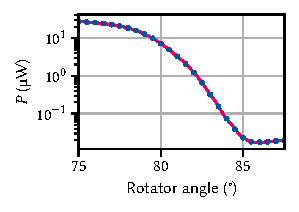
\includegraphics{img/pdf/experiment/power_calibration}
    \caption[\imgsource{img/py/experiment/calibration.py}]{
        Power calibration using the continuously variable \acrshort{nd} filter.
        Error bars from statistics are too small to see.
        Magenta line is a quadratic smoothing spline.
    }
    \label{fig:exp:mjolnir:power_calibration}
\end{marginfigure}

As performing the full calibration is quite time-consuming and furthermore the inversion not fully reliable, the \code{"fast"} calibration update mode sets the rotator angle by performing a noisy optimization.
Here, first the last valid full calibration is loaded and its spline scaled to the current power level.
Then, the residual sum of squares between the target power and the power meter reading is minimized using the \code{noisyopt} package~\cite{Mayer2016} with the starting value given by the angle predicted by the rescaled calibration spline.

\subsection{Rejection feedback}\label{subsec:sec:exp:mjolnir:calibration:rejection}
The excitation rejection by means of cross-polarization extinction has already been discussed in \cref{subsec:setup:optics:coupling:rejection}.
As shown there, the \gls{od} achieved by cross-polarizing the excitation beam with the analyzer mounted in the detection path reaches a maximum close to \num{6} and is extremely sensitive to small variations in the angles of the \quarterwave- and \halfwave-plates controlling polarization state.
Close to the optimum, the \gls{od} is well-described by a parabola as function of those angles, with a second-order polynomial coefficient on the order of \qty[per-mode = symbol]{-0.15}{\per\square\milli\txtdegree}.
Since the optics including the waveplates display chromatic dispersion, the excitation rejection needs to be re-optimized whenever the laser wavelength is changed, and the exponential angular dependence of the transmitted intensity places high demands on the dynamic range of the photo-detector used for measurement.
Therefore, the reflected laser intensity is measured with the \gls{apd} signal digitized by the \tagger on the side exit port of the spectrometer.\sidenote{
    The signals from both \glspl{apd} are combined to achieve the best \gls{snr}, see \cref{part:setup}.
}
The \taggershort can reliably cover a count rate range from \qtyrange{1e2}{1e6}{cps}, compared to the \theccd \gls{ccd} covering only \qtyrange{1e3}{1e5}{cps}.

In the \mjolnir package, the calibration is then carried out as a bivariate noisy minimization using \package{noisyopt}~\cite{Mayer2016}.
Upon initialization the power is set to a small value to avoid overexposing the detectors.
Then, the spectrometer is set to select the laser wavelength, the side exit port is selected, and the optimization over the \quarterwave- and \halfwave-angles is run within conservatively set bounds of $[\qty{-2.5}{\degree}, \qty{2.5}{\degree}]$, which has been found to be a good compromise of robustness and convergence speed.
A caching mechanism stores the optimal angles together with the current wavelength, which serves as a starting guess upon subsequent calibration runs.
The calibration is quite tedious and time-consuming for several reasons.
Chiefly, moving the waveplate angles is slow simply because it is a mechanical movement, and optimizers typically do not take into account the distance between subsequent sample points, potentially resulting in unnecessarily inefficient exploration of the parameter space.
Incorporating a penalty on the sample distance into the optimization algorithm would hence improve the convergence speed.
Additionally, due to vibrations in the cryostat (\cref{ch:setup:vibrations}), the \gls{rms} intensity of the back-scattered laser is large -- and larger the closer the excitation rejection is to its optimal value\sidenote{
    The count rate can vary by up to a factor of two with the frequency of the \gls{ptr} pulses.
} -- and thus requires long averaging times for a robust measurement.
Finally, the algorithm outlined above fails when the starting guess is too far away from the optimum, such as when the new wavelength is on the order of tens of \unit{nm} away from the previously optimized one.
A good -- albeit time-consuming -- strategy is then to incrementally update the wavelength.

\section{Measurement routines}\label{sec:exp:mjolnir:measurement}
Measurements in \mjolnir use the \qcodes infrastructure for data acquisition and storage.
To abstract away code for repetitive setup and teardown tasks, the user interacts with a \code{MeasurementHandler} object through the \code{measure()} method.
The class can be subclassed to customize the aforementioned tasks for different types of experiments (such as those that involve illumination with the laser and detection with the \gls{ccd}, \code{LaserCcdMeasurementHandler}), or add default parameters to every measurement (such as leakage currents or the laser power).
A measurement's independent parameters are passed to \code{measure()} as instances of a \code{Sweep} class which completely determines the measurement structure.
\code{Sweep} objects support syntactic sugar for concatenation (\code{@}), nesting (\code{|}), and parallelization (\code{&}).
Dependent parameters (those that should be measured) can be simple parameters or instances of a \code{Measure} class.\sidenote{
    Besides some optimization for measurements of parameters delegating from the same physical parameter, the latter exists mostly for (primitive) live plotting.
}
The state of external parameters, that is, parameters that are not varied or measured during a measurement, can be defined for the duration of the measurement using the \code{parameter_contexts} argument, a mapping from \qcodes parameters to valid values thereof.
This uses the \code{Parameter.set_to()} context manager to set the parameters to the given values before the measurement starts and restore their original values upon exit in a controlled manner, allowing users to ensure their device is in a well-defined state.
Custom setup and teardown tasks can furthermore be specified through the \code{add_before_run} and \code{add_after_run} arguments, respectively.

\begin{listing}[htpb]
    \begin{pycode}
        from mjolnir.measurement.handler import LaserCcdMeasurementHandler
        from mjolnir.measurement.sweeps import GridSweep
        from mjolnir.measurement.measures import Measure

        handler = LaserCcdMeasurementHandler(station)

        # excitation_path, sample are instances of the ExcitationPath and
        # TrapSample classes, respectively
        power_sweep = GridSweep(excitation_path.power_at_sample,
                                rng=(5e-9, 5e-7), num_points=11,
                                spacing='geom')
        gate_sweep = GridSweep(sample.trap.central_difference_mode,
                               rng=(-2, -1), num_points=51))

        # two-dimensional sweep over power and gate voltage
        sweeps = power_sweep | gate_sweep
        # keep track of the MXC temperature
        measures = sample.fridge.T8

        dataset = handler.measure(
            sweeps,
            measures,
            parameter_contexts={
                sample.trap.central_common_mode: -1,
                detection_path.central_wavelength: 825,
            },
            exposure_time=2
        )
    \end{pycode}
    \caption[\mjolnir measurement workflow]{
    Setup and measurement workflow using the \mjolnir package.
        \code{station} is a \qcodes \code{Station} object managing the instruments.
        The \code{sweeps} object describes a nested loop on whose inner iteration the difference mode parameter of the trap's central gate is swept over a linear grid and on whose outer iteration the laser power, adjusted for the \acrlong{bs} ratio, is swept over a logarithmically spaced grid.
        No dependent parameters (\code{Measure} objects) need to be explicitly specified as the \code{LaserCcdMeasurementHandler} measures the \gls{ccd} spectrum as well as laser power and leakage currents of the swept gates by default.
        The \code{parameter_contexts} argument is used to set the spectrometer wavelength to \qty{825}{\nano\meter} and the common mode voltage of the active trap to \qty{-1}{\volt}.
        The \code{exposure_time} argument is passed through to the \code{initialize} method, where it is used to set up the \gls{ccd} for acquisition.
    }
    \label{lst:exp:mjolnir:workflow}
\end{listing}

A typical workflow for a \gls{pl} measurement using laser and \gls{ccd} is sketched in \cref{lst:exp:mjolnir:workflow}.
The \code{MeasurementHandler} object automatically takes care of, among other things, arming the \gls{ccd}, acquiring a background image in the dark, and opening the laser shutter for the duration of the measurement.
Acquired data is saved to the \qcodes database, but a helper function exporting to the \xarray \code{Dataset} format is available.
Saved together with the data are a snapshot of the \qcodes \code{Station} as well as arbitrary custom metadata.
More details and examples on the measurement functionality can be found in the \sidehref{https://qutech.pages.git-ce.rwth-aachen.de/lab_software/python-mjolnir/}{documentation.}
Lastly, I note that the measurement functionality in \mjolnir is independent of the instrument abstraction and calibration logic and as such could be replaced or augmented with minimal effort by that of other \qcodes-based frameworks such as \package{quantify} or \package{labcore} to make use of their infrastructure.
I leave this option for future work.

\section{Plotting}\label{sec:exp:mjolnir:plotting}
\begin{figure*}
    \centering
    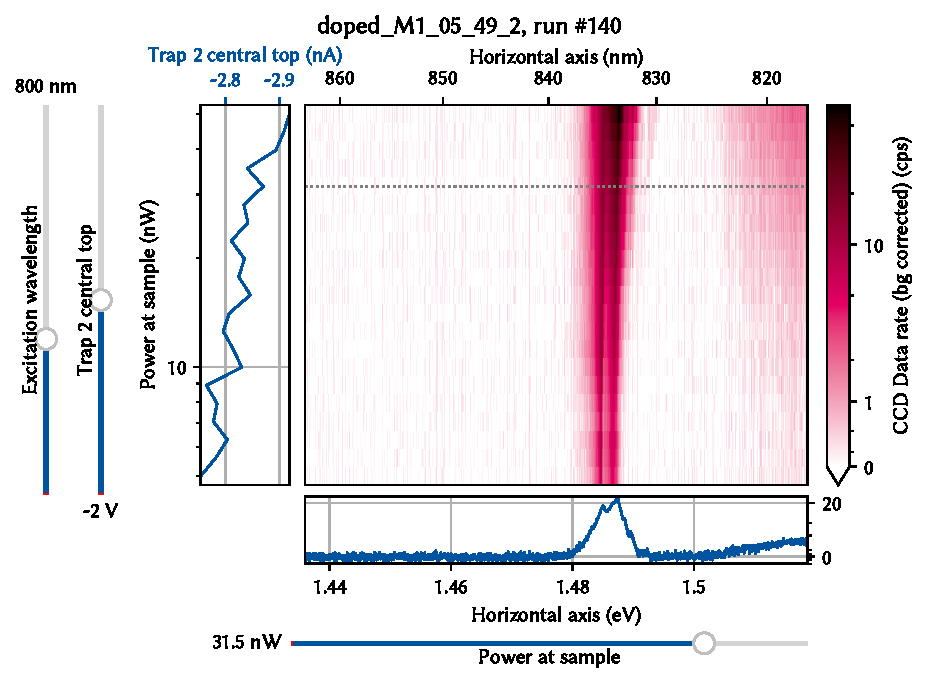
\includegraphics{img/pdf/experiment/plot_nd}
    \caption[\imgsource{img/py/experiment/pl.py}]{
        The \code{plot_nd()} plot window.
        The bottom panel, enabled by default, shows a horizontal line cut through the 2D data of the main panel whose $y$-value can be set with the adjacent slider widget.
        The left panel shows the leakage currents of gates that participate in the sweep and, if measured, the laser power.
        A vertical slider widget is added for each data dimension not displayed on the $x$ or $y$ axis of the main plot.
        The figure title shows the sample as well as the measurement identifiers assigned by \qcodes.
    }
    \label{fig:exp:mjolnir:plot_nd}
\end{figure*}

Optical measurements using \mjolnir often produce multi-dimensional datasets by virtue of the default parameter measured, the \gls{ccd} spectrum, being vector-valued or \emph{batched}.
To visualize such datasets with more than two dimensions, \mjolnir provides the \code{plot_nd()} function that plots 2D slices through the data as a false-color image and generates interactive slider widgets that allow users to modify the slice coordinates.
This facilitates interactively exploring large datasets and recognizing trends present in the data beyond two dimensions.
\Cref{fig:exp:mjolnir:plot_nd} shows an exemplary plot window for a four-dimensional data set obtained from a \gls{ccd} measurement sweeping laser wavelength, power, and a gate voltage, with \cref{lst:exp:mjolnir:plot_nd} showing the code necessary to produce the plot.

\begin{listing}
    \begin{pycode}
        import matplotlib as mpl
        from mjolnir.plotting import plot_nd

        fig, axes, sliders = plot_nd(
            dataset_or_run_id=140, vertical_target='power_at_sample',
            yscale='log^\prime, norm=mpl.colors.AsinhNorm(vmin=0),
            fig_kw=dict(figsize=(6.33585, 4.6))
        )
    \end{pycode}
    \caption[\texttt{plot_nd()} example]{
        Code to produce the plot shown in \cref{fig:exp:mjolnir:plot_nd}.
        If \code{dataset_or_run_id} is an integer, the currently connected \qcodes database is queried for this run identifier.
        Otherwise, it should be an \xarray \code{Dataset}.
    }
    \label{lst:exp:mjolnir:plot_nd}
\end{listing}

The plotting functionality is implemented using \matplotlib.
While not the most performant library, its flexibility in decorating and customizing plots as well as scaling data, such as the $\asinh$-scale normalization used in \cref{fig:exp:mjolnir:plot_nd}, made it the preferred choice.
To nonetheless improve the responsivity of the interactive elements, the plotted artists are \emph{blitted}\sidenote{
    Blitting refers to storing constant backgrounds of raster graphics and only redrawing changing elements.
    See the \matplotlib \href{https://matplotlib.org/stable/users/explain/animations/blitting.html}{documentation}.
}
using the \code{qutil.plotting.BlitManager} class from the \qutil library~\cite{Hangleiter_qutil}.
The data variable to be shown in the main panel can be selected with the \code{array_target} argument, which accepts a string and chooses the closest match in the dataset since the full parameter names are often a bit unwieldy.
Similarly, the coordinates to be plotted on the $x$- and $y$-axes are selected with the \code{horizontal_target} and \code{vertical_target} arguments, respectively.

In addition to plotting measurement data, \mjolnir implements live plotting of instrument data leveraging the \code{qutil.plotting.live_view} module.
Since most instruments do not support multiple concurrent connections, switching control between the \python console and the \gls{gui} program provided by the manufacturer can often be tedious.\sidenote{
    For instance, the \gls{ccd} \gls{gui}, Andor Solis, by default disables the thermoelectric cooler when exiting the program.
}
Thus, making use of their continuous data acquisition functionality is prohibitively time-consuming, but at the same time optical experiments frequently call for live observation of instrument data, for example when aligning the optics.
Live plotting is currently implemented for three different instruments and corresponding parameters; the \thorlabspowermeter power meter (power reading), the \theccd \gls{ccd} (spectrum or image), and the \tagger counting card (count rate(s)).
Data acquisition is executed in a background thread while the plot, implemented in \matplotlib, currently runs in the main thread, and hence does not update while the interpreter is blocked.
In principle, though, the \code{live_view} module also supports plotting in a separate process, making a multiprocessing implementation straightforward.
Interactive \gls{gui} elements in the \matplotlib figure allow for pausing and automatically rescaling the data.\sidenote{
    These two features can also be activated with the \textsc{space} and \textsc{r} keys.
}
Since for the \gls{ccd} data acquisition runs using the \emph{run till abort} mode of the device and as such continuously, the instrument is blocked for the duration of the live plot and it therefore needs to be closed before starting a measurement.
By contrast, the power meter and \taggershort parameters are simply queried regularly in sequential mode and can hence in principle remain open and running while performing measurements.
% mainfile: ../../main.tex
\chapter{Observations}\label{ch:exp:observations}
\AutoLettrine{Pidgeons}
\section{Transfer-matrix method simulations of the membrane structure}\label{sec:exp:tmm}
The \gls{tmm} is a computationally efficient method of obtaining the electric field in layered structures.
In this section, I perform simulations of the heterostructure membranes investigated in \thispart using the \pymoosh package~\cite{Langevin2024} to elucidate the observed quenching of \gls{pl} when illuminating gate electrodes as well as the overall optical efficiency.\sidenote{
    Strictly speaking, the term \acrshort{tmm} only refers to one of the several formalisms implemented in the \pymoosh package.
    While fast, it is not the most numerically stable, and other methods may be preferred if wall time is not a limiting issue.
}
I will first briefly recap the simulation method following \citer{Langevin2024}.
For more details, refer to \ibid and references therein.

Consider a layered structure along $z$ with interfaces at $z_i, i\in\lbrace 0, 1, \dotsc, N+1\rbrace$ that is translationally invariant along $x$ and $y$.
Each layer $i$ may consist of a different dielectric material characterized by a (complex) relative permittivity $\epsilon_{r,i}$.\sidenote{
    We disregard magnetic materials with relative permeability $\mu_r\neq 1$ for simplicity.
}
The electric field component along $y$ of an electromagnetic wave \gls{te} mode originating in some far away point satisfies the Helmholtz equation
\begin{equation}\label{eq:exp:tmm:helmholtz}
    \pdv[2]{E_y}{z} + \gamma_i^2 E_y = 0,
\end{equation}
where $\gamma_i = \sqrt{\epsilon_{r,i}k_0^2 - k_x^2}$ with $k_0=\flatfrac{\omega}{c}$ the wave vector in vacuum and $k_x$ the component along $x$.
In layer $i$ of the structure, the solution to \cref{eq:exp:tmm:helmholtz} may be written as a superposition of plane waves incident and reflected on the lower and upper interfaces~\cite{Langevin2024},
\begin{equation}\label{eq:exp:tmm:fields}
    \begin{dcases}
        E_{y,i}(z) = A_i^{+}\exp{\i\gamma_i[z-z_{i}]} + B_i^{+}\exp{-\i\gamma_i[z-z_{i}]}, \\
        E_{y,i}(z) = A_i^{-}\exp{\i\gamma_i[z-z_{i+1}]} + B_i^{-}\exp{-\i\gamma_i[z-z_{i+1}]},
    \end{dcases}
\end{equation}
where the coefficients with superscript $+$ ($-$) are referenced to the phase at the upper (lower) interface, respectively.
Matching these solutions at $z=z_i$ for all $i$ to satisfy the interface conditions imposed by Maxwell's equations gives rise to a linear system of equations, the solution to which can be obtained through several different methods.

A particularly simple method is the \acrlong{tmm} ($T$-matrix formalism), which corresponds to writing the interface conditions at $z=z_i$ as the matrix equation
\begin{equation}\label{eq:exp:tmm:interface}
    \pmqty{A_{i+1}^{+}\\B_{i+1}^{+}} = T_{i,i+1}\pmqty{A_{i}^{-}\\B_{i}^{-}}
\end{equation}
with
\begin{equation}\label{eq:exp:tmm:T}
    T_{i,i+1} = \frac{1}{2\gamma_{i+1}}\begin{pmatrix}
        \gamma_{i} + \gamma_{i+1} & \gamma_{i} - \gamma_{i+1} \\
        \gamma_{i} - \gamma_{i+1} & \gamma_{i} + \gamma_{i+1}
    \end{pmatrix}
\end{equation}
the transfer matrix for interface $i$.
Connecting the coefficients for adjacent interfaces within a layer of height $h_i = z_{i+1} - z_{i}$ requires propagating the phase,
\begin{equation}\label{eq:exp:tmm:propagation}
    \pmqty{A_{i}^{-}\\B_{i}^{-}} = C_{i}\pmqty{A_{i}^{+}\\B_{i}^{+}},
\end{equation}
with
\begin{equation}\label{eq:exp:tmm:C}
    C_{i} = \exp\left\lbrace\diag(-\i\gamma_i h_i, \i\gamma_i h_i)\right\rbrace.
\end{equation}
Iterating \cref{eq:exp:tmm:C,eq:exp:tmm:T}, the total transfer matrix $T = T_{0,N+1}$ then reduces to the matrix product
\begin{equation}\label{eq:exp:tmm:T:total}
    T = T_{N,N+1}\prod_{i=0}^{N-1} T_{i,i+1} C_i.
\end{equation}
From $T$, the reflection and transmission coefficients can be obtained as $r=A_0^{-}=-\flatfrac{T_{01}}{T_{00}}$ and $t=B_{N+1}^{+}=rT_{10} + T_{11}$.
Taking the absolute value square of reflection and transmission coefficients then yields the reflectance \reflectance and the transmittance \transmittance, which correspond to the fraction of total incident power being reflected and transmitted, respectively.
To obtain the absorptance \absorptance, the fraction of power being absorbed, in layer $i$, one can compute the difference of the $z$-components of the Poynting vectors (\cf \cref{eq:setup:optics:coupling:poynting}) at the top of layers $i$ and $i+1$.
In the \gls{te} case considered here, \cref{eq:setup:optics:coupling:poynting} reduces to~\cite{Langevin2024}
\begin{equation}\label{eq:exp:tmm:poynting}
    \bvec{S}_i = \re\left[\frac{\gamma_i^{\ast}}{\gamma_0}\left(A_i^{+} - B_i^{+}\right)^{\ast}\left(A_i^{+} + B_i^{+}\right)\right]
\end{equation}
and is hence straightforward to extract from the calculation of either the $S$ or $T$ matrices.

\Cref{eq:exp:tmm:T:total} is simple to evaluate on a computer, making this method attractive for numerical applications.
However, the opposite signs in the argument of the exponentials in \cref{eq:exp:tmm:C} can lead to instabilities for evanescent waves ($\gamma_i\in\mathbb{C}$) due to finite-precision floating point arithmetic~\cite{Duetz}.
Rewriting \cref{eq:exp:tmm:T} to have incoming and outgoing fields on opposite sides of the equality alleviates this issue while sacrificing the simple matrix-multiplication composition rule in what is known as the scattering matrix ($S$-matrix) formalism.
Finally, note that for a thorough accounting of in- and out-going field amplitudes, excitonic effects should be included, for example using the approach by \citet{DAndrea1990}.

Beyond the calculation of the aforementioned coefficients, the \gls{tmm} formalism also allows to compute the full spatial dependence of the fields.
Two cases are implemented in \pymoosh: irradiation of the layered structured with a Gaussian beam rather than plane waves of infinite extent, and a current line source inside the structure.
In the first case, the previously assumed translational invariance along $x$ leading to a plane-wave spatial dependence is replaced by a superposition of plane waves weighted with a normally distributed amplitude,\sidenote{
    \Ie, the inverse Fourier transform of $\mc{E}_0(k_x) E_{y,i}(k_x, z)$.
}
\begin{equation}\label{eq:exp:tmm:gauss:x}
    E_{y,i}(x,z) = \exp(\i k_x x)\rightarrow \int\ddf{k_x}\mc{E}_0(k_x) E_{y,i}(k_x, z)\exp(\i k_x x),
\end{equation}
with (\cf \cref{eq:setup:gaussian})
\begin{equation}\label{eq:exp:tmm:gauss:ampl}
    \mc{E}_0(k_x) = \frac{w_0}{2\sqrt{\pi}}\exp\left\lbrace - \i k_x x_0 -\left[\frac{w_0 k_x}{2}\right]^2\right\rbrace
\end{equation}
and
\begin{equation}\label{eq:exp:tmm:gauss:z}
    E_{y,i}(k_x, z) = A_{i}^{-}\exp\lbrace\i\gamma_i(k_x)[z-z_{i+1}]\rbrace + B_{i}^{+}\exp\lbrace -\i\gamma_i(k_x)[z-z_{i}]\rbrace,
\end{equation}
and where we considered only normal incidence for simplicity.

In the second case, \citet{Langevin2024} consider an AC current $I$ flowing through a translationally invariant, one-dimensional wire along $y$ at $x=x_{\mr{s}}$.
This introduces a source term into the Helmholtz equation \cref{eq:exp:tmm:helmholtz} which, upon Fourier transforming in $x$ direction, leads to
\begin{equation}\label{eq:exp:tmm:helmholtz:green}
    \pdv[2]{\hat{E}_y}{z} + \gamma_i^2\hat{E}_y = -\i\omega\mu_0 I\delta(z)\exp(\i k_x x_{\mr{s}}).
\end{equation}
The electric field $\hat{E}_{y,i}(k_x, z)$ is thus proportional to the Green's function of \cref{eq:exp:tmm:helmholtz:green} and can be obtained using a similar procedure as in the case of a distant source incident on the structure by matching the interface conditions.
Performing the inverse Fourier transform by means of \cref{eq:exp:tmm:gauss:x} with constant weights, $\mc{E}_0(k_x)\equiv 1$, then yields the two-dimensional spatial distribution of the electric field, $E_{y,i}(x, z)$.

\begin{figure}
    \centering
    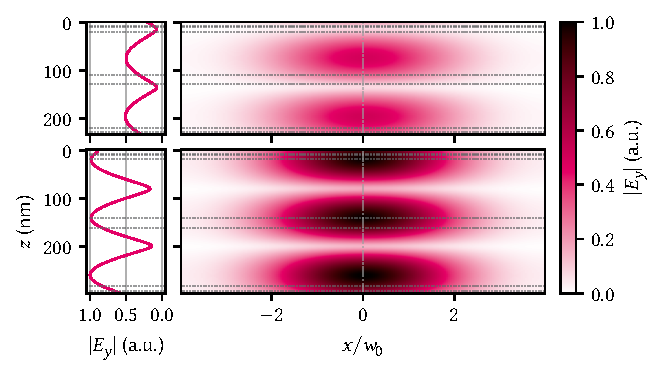
\includegraphics{img/pdf/experiment/tmm_field}
    \caption[\imgsource{img/py/experiment/tmm.py}]{
        Absolute value of the electric field inside the double-gated heterostructure under illumination with a Gaussian beam at $\lambda=\qty{825}{\nano\meter}$ from the top.
        Top (bottom) panels show the structure with the default (optimized) barrier thickness of \qty{90}{\nano\meter} (\qty{122}{\nano\meter}), respectively.
        Dotted horizontal lines indicate interfaces between different materials while the vertical dash-dotted line indicates the position of the line cuts shown in the left column.
        Increasing the thickness of the barrier has two beneficial effects; first, the overall field intensity inside the structure is higher by a factor of two, and second, there is a peak rather than a knot in the \gls{qw} at a depth of $\sim\qty{120}{\nano\meter}$ ($\sim\qty{150}{\nano\meter}$), leading to enhanced absorption.
    }
    \label{fig:exp:tmm:field}
\end{figure}

\begin{margintable}
    \centering
    \footnotesize
    \caption{
        Absorptance $\mathscr{A}$ and reflectance $\mathscr{R}$ in the \gls{qw} for different configurations of the heterostructure.
        \enquote{Bare} is the standard structure without gate electrodes.
        \enquote{TG} and \enquote{BG} are with a gate on either the top or bottom side.
        \enquote{TG+BG} is with gates on both sides as on a trap site.
    }
    \label{tab:exp:tmm:absorptance_reflectance}
    % This table is automatically generated by img/py/experiment/tmm.py
\begin{tabular}{lSS}
\toprule
 & {$\mathscr{A}$ (\unit{\percent})} & {$\mathscr{R}$ (\unit{\percent})} \\
\midrule
Bare & 2.9 & 22.4 \\
TG & 1.8 & 42.0 \\
BG & 0.5 & 82.7 \\
TG+BG & 0.4 & 84.8 \\
\bottomrule
\end{tabular}

\end{margintable}

\begin{marginfigure}
    \centering
    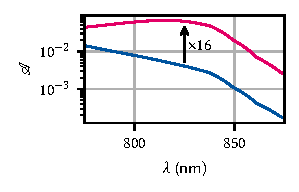
\includegraphics{img/pdf/experiment/tmm_absorptance}
    \caption[\imgsource{img/py/experiment/tmm.py}]{
        \Gls{qw} absorptance \absorptance in a heterostructure with default (blue) and optimized (magenta) barrier thickness and top and bottom gates as function of wavelength.
        Optimization was performed at \qty{825}{\nano\meter} using the differential evolution algorithm implemented in \pymoosh, resulting in a barrier thickness of \qty{122}{\nano\meter} and an absorptance better by a factor of \num{16} at \qty{6.3}{\percent}.
    }
    \label{fig:exp:tmm:wavelengths}
\end{marginfigure}
\clearpage
\begin{marginfigure}
    \centering
    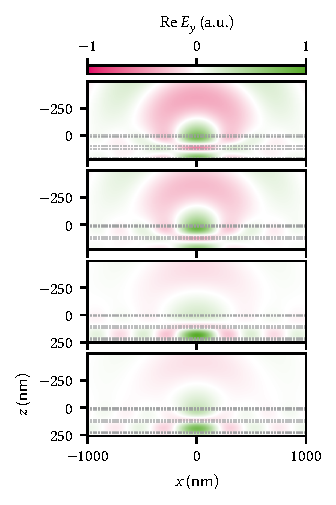
\includegraphics{img/pdf/experiment/tmm_green}
    \caption[\imgsource{img/py/experiment/tmm.py}]{
        Real part of the electric field emitted by a current line located in the \gls{qw} (black point) for different cases of the unoptimized structure.
        From top to bottom: bare heterostructure, top gate, bottom gate, top and bottom gate.
        The half space $z<0$ is the air above the membrane in the direction of the objective lens and the dotted lines indicate interfaces between materials.
        Evidently, the bottom gate reduces the amplitude in the upper half of the membrane and thereby the outcoupling efficiency compared to the structures with just a top gate, consistent with what is observed in the experiment.
    }
    \label{fig:exp:tmm:green}
\end{marginfigure}

\begin{marginfigure}
    \centering
    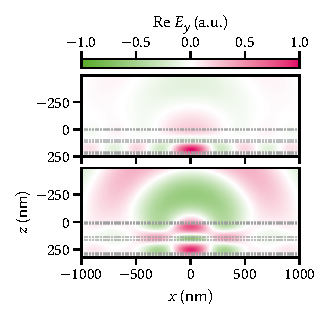
\includegraphics{img/pdf/experiment/tmm_green_opt_tgbg}
    \caption[\imgsource{img/py/experiment/tmm.py}]{
        Real part of the electric field emitted by a current line located in the \gls{qw} (black point) for the default (top) and optimized (bottom) structures with top and bottom gates.
        Optimizing the barrier thickness for absorption in the \gls{qw} evidently also drastically improves the outcoupling efficiency into the halfspace $z<0$.
    }
    \label{fig:exp:tmm:green:opt:tgbg}
\end{marginfigure}
\clearpage

\begin{marginfigure}
    \centering
    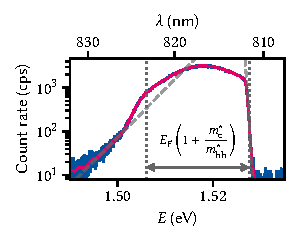
\includegraphics{img/pdf/experiment/2deg_pl}
    \caption[
        \sampleid{Doped M1_05_49-2}
        \thewavelength{795}.
        \thepower{0.92}{\micro}
        \protect\newline
        \imgsource{img/py/experiment/pl.py}
    ]{
        \Gls{pl} of the bare \gls{2deg}.
        Magenta line is a smoothing spline fit to the data.
        Indicated by dotted gray lines are the Fermi edge at high and the band edge at low energy.
        The Fermi edge has a Fermi distribution (exponential indicated by a dashed gray line) whose temperature is typically much higher than the lattice temperature ($\sim\qty{1}{\kelvin}$).
        Below the band edge there is an exponential tail (dashed gray line) due to impurities that permeates far into the gap.
    }
    \label{fig:exp:pl:2deg}
\end{marginfigure}

\Cref{fig:exp:pl:2deg} shows a typical \gls{pl} spectrum obtained on the bare, unbiased \gls{qw} of a doped membrane sample.
This measurement corresponds to the configuration already discussed in \cref{fig:exp:theory:bandstructure:doped}.
Due to the Pauli exclusion principle, electrons require an energy of at least $E_\mr{F}\left(1 + m_{\mr{c}}^\ast/m_{\mr{hh}}^\ast\right)$ above the band gap and, because of the vanishingly small photon momentum, a momentum of at least $k_\mr{F}$ to be excited into a free state above the Fermi level $\mu$ (dotted gray line).\sidenote{
    This is known as the Burstein-Moss shift~\cite{Burstein1954,Moss1954}.
}
Once excited, they quickly relax down to the Fermi edge at $\mu$ from where they can recombine emitting a photon.
As the Fermi sea is at a finite temperature, the high-energy shoulder of the \gls{pl} spectrum is hence thermally broadened according to the Fermi distribution function of the electron gas (dashed gray line).
The associated temperature is around \qty{1.5}{\kelvin} and hence orders of magnitude higher than the lattice temperature of \qty{10}{\milli\kelvin}.
This effect has already been observed by \citet{Pinczuk1984}.
Like in those experiments, the temperature of the Fermi edge does not vary significantly with excitation power, making carrier heating due to high excitation power an unlikely cause~\cite{Ulbrich1973}.

\Gls{pl} emission is possible also at lower energies as electrons inside the Fermi sea recombine with the free photo-hole that scatters towards the valence band ege.
The band gap then defines the low-energy shoulder of the \gls{pl} spectrum, below which there are -- ideally -- no states available (dotted gray line).
However, the \gls{pl} reveals there are indeed free states decaying exponentially into the gap, originating most likely from impurities (dashed gray line).
Compared to the results of \citet{Kamburov2017}, the \gls{pl} spectra obtained here are much flatter over energy, with the \gls{pl} peak typically close to the middle between gap and Fermi edge.
Conversely, \citet{Kamburov2017} observed a strong peak at the band gap,\sidenote{
    \Cf also \citet{Gabbay2008}, who observe all but no \gls{fes} in samples nominally comparable to ours.
}
indicating that in our samples holes are more strongly localized and therefore have a wider spread in $k$-space, enabling transitions in a wider range of wave vectors~\cite{Skolnick1987}.
This would in turn imply increased alloy disorder or interface roughness~\cite{Gabbay2008}, an observation we shall come back to in \cref{ch:exp:observations}. % TODO: ref multiplets

From the width of the \gls{2deg} emission, we can calculate the charge carrier density by relating it to the Fermi energy in two dimensions~\cite{Pinczuk1984,Ihn2009},
\begin{equation}\label{eq:exp:pl:n}
    n = \frac{m^{\ast}_{\mr{c}}E_{\mr{F}}}{\pi\hbar^2} = \frac{\mu\Delta E}{\pi\hbar^2},
\end{equation}
where $\Delta E$ is the bandwidth of the emission (dashed gray lines in \cref{fig:exp:pl:2deg}) and $\mu = m^{\ast}_{\mr{c}}m^{\ast}_{\mr{hh}}/(m^{\ast}_{\mr{c}} + m^{\ast}_{\mr{hh}})$ is the reduced mass of conduction and valence band.
For this particular sample, \cref{eq:exp:pl:n} yields $n = \qty{5e11}{\per\square\centi\meter}$ or, equivalently, $E_{\mr{F}} = \qty{18}{\milli\electronvolt}$ and $k_{\mr{F}} = \qty{1.8e8}{\per\meter}$.
Comparing this value to that obtained from a simulation of the heterostructure with nominal doping concentration $N_{\mr{d}} = \qty{6.5e17}{\per\cubic\centi\meter}$ using a self-consistent Poisson-Schrödinger solver~\cite{PoissonSchroedinger}, $n = \qty{1.4e11}{\per\square\centi\meter}$, shows a significant discrepancy indicating a severe mismatch between nominal and actual doping concentrations.\sidenote{
    Note that the carrier density obtained thus does not vary significantly with excitation power, ruling out photo-doping as a source of the discrepancy.
    See \cref{ch:app:exp:observations} for a measurement of the \gls{2deg} \gls{pl} as function of power.
}
Finally, we observe that the gap according to the preceding analysis is redshifted from the undoped bulk gap of \qty{1.519}{\electronvolt}~\cite{Vurgaftman2001} by \qty{13}{\milli\electronvolt}.\sidenote{
    The redshift is in fact larger still due to the confinement energy of the \gls{qw}, estimated to be $\qty{17}{\milli\electronvolt}$ in \cref{sec:exp:theory:qcse}.
}
\Citet{Descamps2021} hypothesized that the removal of the \ch{GaAs} substrate and the associated change in strain leads to this lowering of the band gap.
However, this effect was also already observed by \citet{Pinczuk1984} in \enquote{bulk} modulation-doped \ch{GaAs} \glspl{qw}.
There, the authors put forth a renormalization of the band gap due to many-body interactions as an explanation.
Indeed, it is likely just bandgap narrowing due to doping~\cite{Jain1992}.

\begin{figure}
    \centering
    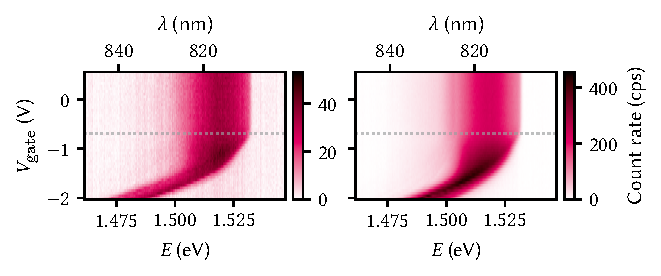
\includegraphics{img/pdf/experiment/honey_H13_stark_shift_vs_gate}
    \caption[
        \sampleid{Honey H13}
        \thewavelength{795},
        \thepower{1}{\micro}.
        \protect\newline
        \imgsource{img/py/experiment/pl.py}
    ]{
        \Gls{pl} as function of gate voltage on a single fan-out gate on the bottom (left) and top (right) side of the membrane.
        The behavior is qualitatively similar but the overall quantum efficiency lower by an order of magnitude for gates on the bottom (as-grown buried) side.
    }
    \label{fig:exp:pl:honey_H13_stark_shift_vs_gate}
\end{figure}

\begin{marginfigure}
    \centering
    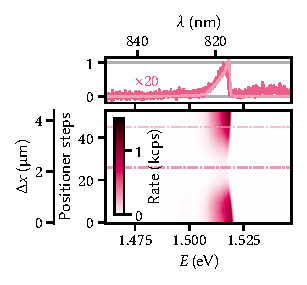
\includegraphics{img/pdf/experiment/fig_F10_positioning}
    \caption[
        \sampleid{Fig F10}
        \thewavelength{795}.
        \protect\newline
        \imgsource{img/py/experiment/pl.py}
    ]{
        \Gls{pl} of the unbiased \gls{qw} as the laser is stepped across a bottom gate.
        The line traces in the upper panel are taken at the positions indicated by dash-dotted lines.
        Positioner steps are converted to distance using a linear fit of the positioner readout after the initial hysteresis has worn off (about \num{10} steps).
        The Fermi edge shows a slight redshift when on top of the gate in this sample.
    }
    \label{fig:exp:pl:fig_F10_positioning}
\end{marginfigure}

\begin{marginfigure}
    \centering
    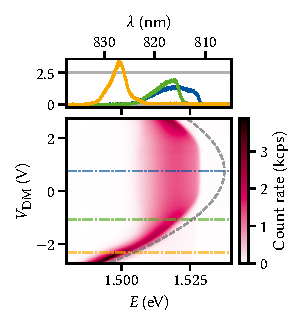
\includegraphics{img/pdf/experiment/doped_M1_05_49-2_difference_mode}
    \caption[
        \sampleid{Doped M1_05_49-2}
        \thevoltage{-1.3}{CM},
        \thewavelength{795}.
        \thepower{10}{\micro}.
        \protect\newline
        \imgsource{img/py/experiment/pl.py}
    ]{
        \Gls{pl} as function of difference-mode voltage on a large exciton trap.
        The observed Stark shift follows roughly the expected quadratic dispersion, but is offset by \qty{0.75}{\volt} with respect to zero bias.
        Dashed gray line is a guide to the eye of a parabola with curvature \qty{-3.5}{\milli\electronvolt\per\volt\squared}.
        Line cuts in the upper panel are taken at the voltages indicated by dash-dotted lines in the lower.
    }
    \label{fig:exp:pl:doped_M1_05_49-2_difference_mode}
\end{marginfigure}

\begin{marginfigure}
    \centering
    \includegraphics{img/pdf/experiment/doped_M1_05_49-2_ple_margin}
    \caption[
        \sampleid{Doped M1_05_49-2}
        \thevoltage{-1.3}{CM},
        \thepower{1}{\micro}.
        \protect\newline
        \imgsource{img/py/experiment/ple.py}
    ]{
    }
    \label{fig:exp:pl:doped_M1_05_49-2_ple_margin}
\end{marginfigure}

\begin{figure}
    \centering
    \includegraphics{img/pdf/experiment/doped_M1_05_49-2_ple_wide}
    \caption[
        \sampleid{Doped M1_05_49-2}
        \thevoltage{-1.3}{CM},
        \thepower{1}{\micro}.
        \protect\newline
        \imgsource{img/py/experiment/ple.py}
    ]{
    }
    \label{fig:exp:pl:doped_M1_05_49-2_ple_wide}
\end{figure}

\begin{figure}
    \centering
    \includegraphics{img/pdf/experiment/doped_M1_05_49-2_ple_delta}
    \caption[
        \sampleid{Doped M1_05_49-2}
        \thevoltage{-1.3}{CM},
        \thepower{1}{\micro}.
        \protect\newline
        \imgsource{img/py/experiment/ple.py}
    ]{
    }
    \label{fig:exp:pl:doped_M1_05_49-2_ple}
\end{figure}

\begin{figure}
    \centering
    \includegraphics{img/pdf/experiment/doped_M1_05_49-2_ple_cuts}
    \caption[
        \sampleid{Doped M1_05_49-2}
        \thevoltage{-1.3}{CM},
        \thepower{1}{\micro}.
        \protect\newline
        \imgsource{img/py/experiment/ple.py}
    ]{
        \Gls{pl} (solid lines) and \gls{ple} (dashed lines) for different voltages $V_{\mr{DM}}$ (\cf \cref{fig:exp:pl:doped_M1_05_49-2_difference_mode}).
        The \gls{ple} data points correspond to \gls{pl} spectra integrated up to the laser line.
        Arrows indicate the Stokes shift $\Delta E_{\mr{S}}$, which is approximately constant (although assignment of the gap peak is difficult for \qtylist{1.57;0}{\volt}) until the \gls{2deg} is fully depleted and the exciton resonance shifts quadratically with the electric field.
        The features at \qty{1.555}{\electronvolt} do not shift with the voltage and are thus likely unrelated to the trap.
        For the largest voltage, there is another peak at \qty{1.51}{\electronvolt} whose origin is unclear.
    }
    \label{fig:exp:pl:doped_M1_05_49-2_ple_cuts}
\end{figure}

\begin{figure}
    \centering
    \includegraphics{img/pdf/experiment/doped_M1_05_49-2_ple}
    \caption[
        \sampleid{Doped M1_05_49-2}
        \thevoltage{-1.3}{CM},
        \thepower{1}{\micro}.
        \protect\newline
        \imgsource{img/py/experiment/ple.py}
    ]{
    }
    \label{fig:exp:pl:doped_M1_05_49-2_ple}
\end{figure}

\begin{figure}
    \centering
    \includegraphics{img/pdf/experiment/doped_M1_05_49-2_power}
    \caption[
        \sampleid{Doped M1_05_49-2}
        \thevoltage{-2.7}{DM},
        \thevoltage{-1.3}{CM},
        \thewavelength{795}.
        \protect\newline
        \imgsource{img/py/experiment/pl.py}
    ]{
        \Gls{pl} as function of excitation power $P$ plotted on a logarithmic color scale.
        Two qualitatively different regimes are indicated by dashed gray lines as guides to the eye; below \qty{10}{\nano\watt}, the main peak displays a blueshift logarithmic in excitation power, $E = \qty{1.485}{\electronvolt} + \qty{5}{\milli\electronvolt}\log_{10} P$.
        Above, the blueshift diminishes significantly.
        Three additional lines, indicated by arrows, with varying power dispersion appear.
    }
    \label{fig:}
\end{figure}

\begin{figure*}
    \centering
    \includegraphics{img/pdf/experiment/doped_M1_05_49-2_multiplets}
    \caption[
        \sampleid{Doped M1_05_49-2}
        \thevoltage{0}{B}.
        \protect\newline
        \imgsource{img/py/experiment/pl.py}
    ]{
        Wide-range \gls{pl} parameter sweep on a large exciton trap plotted as function of excitation power and detection energy.
        Rows are data for three different excitation wavelengths, columns for four different top gate voltages $V_{\mr{T}}$ and share color and line cut scales.
        Line cuts are taken at the indicated positions of $P = \qtylist{7;16;35}{\nano\watt}$ and drawn scaled by the fraction of excitation power with respect to \qty{35}{\nano\watt}.
        % Atomic step fluctuations would shift by ~900 μeV (a = 5.6 Α)
    }
    \label{fig:exp:pl:doped_M1_05_49-2_multiplets}
\end{figure*}

% mainfile: ../../main.tex
\chapter{Conclusion \& outlook}\label{ch:exp:conclusion}
\AutoLettrine{Dogs}

\cite{Baeten2015,Glazov2020,Huang2023b}

\pagelayout{wide} % No margins
\part{A Filter-Function Formalism For Unital Quantum Operations}
\label{part:ff}
\pagelayout{margin} % Restore margins
\glsresetall

% mainfile: ../../main.tex
\chapter{Introduction}\label{ch:ff:introduction}
\begin{partcontribs}
    \Thispart is based to large extent on \sideciter{Hangleiter2021}, an early draft of which in turn was my Master's thesis~\sidecite{Hangleiter2019}, and as such contains text written by all three authors.
    \Cref{ch:ff:examples,sec:app:ff:time_domain_methods} additionally contains results published in \sideciter{Cerfontaine2021}.
    Parts of this work have also been included in \sideciter{Cerfontaine2019}.
    % TODO: can we make this nicer?
    Refer to References~\cite[Section 1.3]{Hangleiter2019} and~\cite[Section 3.7]{Cerfontaine2019} for detailed author contributions up to that point.
    \Cref{ch:ff:validation,sec:app:ff:concatenation} contain new results.
\end{partcontribs}
\begin{authornote}
    In Reference~\cite{Hangleiter2021}, extensive use was made of \citeauthor{Kubo1962}'s \emph{cumulant expansion}~\cite{Kubo1962}.
    Due to an error in \citeauthor{Kubo1962}'s paper which was only pointed out several years later~\cite{Fox1976} and we were not aware of, those results turned out to be not exact as claimed but approximate~\sidecite{Hangleiter2024}.\sidenote{
        Unfortunately, the error has proliferated through the literature and proves quite pervasive despite the significant amount of time that has passed since it was first discovered.
        Recent examples include~\citer{Norris2016}.
        One may only speculate if this is because of the 14 years that passed between the original publication and the correction, the lack of an erratum once the mistake had been discovered, or simply because of \citeauthor{Kubo1962}'s fame.
        In any case, it might serve as a cautionary tale and possibly an impetus to a less static publication system that allows, for example, cross-linking commentaries and critiques.
    }
    We address this discrepancy in \cref{ch:ff:validation}.
\end{authornote}
\AutoLettrine{In} the circuit model of quantum computing, computations are driven by applying time-local quantum gates.
Any algorithm can be compiled using sequences of one- and two-qubit gates~\cite{DiVincenzo1995}.
Ideal, error-free gates are represented by unitary transformations, so that simulating the action of an algorithm on an initial state of a quantum computer amounts to simple matrix multiplication.
Real implementations are subject to noise that causes decoherence resulting in gate errors.
If the noise is uncorrelated between gates, its effect can be described by quantum operations acting as linear maps on density matrices, even when several gates are concatenated.
A closely related approach is the use of a master equation in \gls{gksl} form~\cite{Gorini1976,Lindblad1976}, which governs the dynamics of density matrices under the influence of Markovian noise with a flat power spectral density.

Yet many physical systems used as hosts for qubits do not satisfy the condition of uncorrelated noise.
One example frequently encountered in solid-state systems is that of \oneoverf noise, which in principle contains arbitrarily long correlation times.
It emerges for instance as flux noise in superconducting qubits and electrical noise in quantum dot qubits~\cite{Brownnutt2015,Kumar2016a,Yoneda2018,Paladino2014}.
Whereas simple approaches exist to treat for example quasistatic noise, which corresponds to perfectly correlated noise (\ie, a spectrum with weight only at zero frequency), they cannot be applied to \oneoverf noise because of the wide distribution of correlation times it contains~\cite{Connors2022}.
Thus, there is a gap in the mathematical descriptions of gate operations for noises with arbitrary power spectra that exist between the extremal cases of perfectly flat (white) and sharply peaked (quasistatic) spectra.
To capture experimentally relevant effects important to understand the capabilities of quantum computing systems, a universally applicable formalism is hence desirable.
For example, one may expect the fidelity requirements for quantum error correction to be more stringent for correlated noise as errors of different gates can interfere constructively~\cite{Ng2009}.
On the other hand, it might also be possible to use correlation effects to one's benefit, attenuating decoherence by cleverly constructing the gate sequences in algorithms.

As experimental platforms begin to approach fidelity limits set by employing primitive pulse schemes~\cite{Veldhorst2014,Debnath2016,Yoneda2018} and detailed knowledge about noise sources and spectra in solid-state systems becomes available~\cite{Dial2013,Quintana2017,Malinowski2017}, control pulse optimizations tailored towards specific systems will be required to further push fidelities beyond the error correction threshold~\cite{Barends2014,Blume-Kohout2017}.
This calls for flexible and generically applicable tools as a basis for the numerical optimization of pulses as well as the detailed analysis of the quantum processes they effect.
In order to obtain a useful description also for gate operations that decouple from leading orders of noise, such as \glspl{dcg}~\cite{Khodjasteh2009}, beyond leading order results are required.

In \citer{Cerfontaine2021} we presented a formalism based on filter functions and the \gls{me} that addresses these needs and limitations of the canonical master equation approach for correlated noise.
Specifically, we showed how process descriptions can be obtained perturbatively for arbitrary classical noise spectra and derived a concatenation rule to obtain the filter function of a sequence of gates from those of the individual gates.
This work generalizes and extends these results.

\Glspl{ff} were originally introduced to describe the decay of phase coherence under \gls{dd} sequences~\cite{Kofman2001,Martinis2003,Uhrig2007,Cywinski2008} consisting of wait times and perfect $\pi$-pulses.
The formalism facilitated recognizing these sequences as band-pass filters that allow for probing the environmental noise characteristics of a quantum system through noise spectroscopy~\cite{Alvarez2011,Bylander2011,Paz-Silva2017,Malinowski2017} or optimizing sequences to suppress specific noise bands~\cite{Biercuk2009,Uys2009,Soare2014,Malinowski2017}.
It can also be extended to fidelities of gate operations for single~\cite{Green2012,Green2013} or multiple~\cite{Gungordu2018,Ball2020} qubits using the \gls{me}~\cite{Magnus1954,Blanes2009} as well as more general \gls{dd} protocols~\cite{Paz-Silva2014}.
The works by~\citet{Green2013} and~\citet{Clausen2010} also introduced the notion of the control matrix as a quantity closely related to the canonical filter function that is convenient for calculations.
In this context, the formalism's capability to predict fidelities of gate implementations has been identified and experimentally tested~\cite{Green2013,Kabytayev2014,Soare2014,Ball2016}.
More recently, it has also proved useful in assessing the performance requirements for classical control electronics~\cite{VanDijk2019}.

While analytical approaches allow for the calculation of filter functions of arbitrary quantum control protocols in principle, it is in practice often a tedious task to determine analytical solutions to the integrals involved if the complexity of the applied wave forms goes beyond simple square pulses or extends to multiple qubits.
Moreover, one does not always have a closed-form expression of the control at hand, such as is the case for numerically optimized control pulses.
This calls for a numerical approach which, while giving up some of the insights an analytical form offers, is universally applicable and eliminates the need for laborious analytical calculations.

Here, we build and extend upon our work of~\citer{Cerfontaine2021} and that of~\citer{Green2013} to show that the formalism can be recast within the framework of stochastic Liouville equations by means of the cumulant expansion~\cite{Kubo1962,Kubo1963,Fox1976,Bianucci2020}.
For Gaussian noise commuting with the control, this entails exact results for the quantum process of an arbitrary control operation using only first and second order terms of the \gls{me}~\cite{Magnus1954}.
If the noise is Gaussian but in general non-commuting, the cumulant expansion does not terminate~\cite{Fox1976}, but we show that the truncation still yields highly accurate results except in the ultralow-frequency regime by computing the exact filter function from random sampling.
Moreover, due to the fact that the \gls{me} retains the algebraic structure of the expanded quantity~\cite{Blanes2009} we are able to separate incoherent and coherent contributions to the quantum process.
We give explicit methods to evaluate these terms for piecewise-constant control pulses.
Moreover, we show that the formalism naturally lends itself as a tool for numerical calculations and present the \filterfunctions \python software package that enables calculating the filter function of arbitrary, piecewise constant defined pulses~\cite{Hangleiter_ff}.
On top of providing methods to handle individual quantum gates, the package also implements the concatenation operation as well as parallelized execution of pulses on different groups of qubits, allowing for a highly modular and hence computationally powerful treatment of quantum algorithms in the presence of correlated noise.
Given an arbitrary, classical noise spectral density, it can be used to calculate a matrix representation of the error process.
From this matrix one can extract average gate fidelities, transition probabilities, and leakage rates as we derive below.
To simplify adaptation the software's \gls{api} is strongly inspired by and compatible with \qutip~\cite{Johansson2012} as well as \qopt~\cite{Teske2022}.
This allows users to use these packages in conjunction.
Assessing the computational performance, we show that our method outperforms \gls{mc} simulations for single gates.
New analytical results applicable to periodic Hamiltonians and employing the concatenation property make this advantage even more pronounced for sequences of gates.
To highlight the main software features, we show example applications below.

We provide this package in the expectation that it will be a useful tool for the community.
Besides recasting and expanding on our earlier introduction of the formalism in~\citer{Cerfontaine2021}, the present work is intended to provide an overview of the software and its capabilities.
It is structured as follows: In \cref{ch:ff:theory} we derive a closed-form expression for unital quantum operations in the presence of non-Markovian Gaussian noise and lay out how it may be evaluated using the filter-function formalism.
We review the concatenation of quantum operations shown in~\citer{Cerfontaine2021} and furthermore adapt the method by~\citet{Green2013} to calculate the filter function of an arbitrary control sequence numerically.
We will specifically focus on computational aspects of the formalism and lay out how to compute various quantities of interest.
Moreover, we classify its computational complexity for calculating average gate fidelities and remark on simplifications that allow for drastic improvements in performance in certain applications.
In \cref{ch:ff:validation}, we validate the truncation of the cumulant expansion after the second order using a random sampling approach to compute the exact filter functions of the noisy quantum process for Gaussian noise.
In \cref{ch:ff:software}, we then introduce the \filterfunctions software package by outlining the programmatic structure and giving a brief overview over the \gls{api}.
Lastly, in \cref{ch:ff:examples}, we show the application of the software by means of four examples that highlight various features of the formalism and its implementation.
Therein, we first demonstrate that the formalism can predict average gate fidelities for complex two-qubit quantum gates in agreement with computationally much more costly \gls{mc} calculations.
Next, we show how it can be applied to periodically driven systems to efficiently analyze Rabi oscillations.
We finally establish the formalism's ability to predict deviations from the simple concatenation of unitary gates for sequences and algorithms in the presence of correlated noise by simulating a \gls{rb} experiment as well as assembling a \gls{qft} circuit from numerically optimized gates.
We conclude by briefly remarking on possible future application and extension of our method in \cref{ch:ff:conclusion}.

Throughout this part we will denote Hilbert-space operators by Roman font, \eg $U$, and quantum operations and their representations as transfer matrices in Liouville space by calligraphic font, \eg \liouvU, which we also use for the control matrix \ctrlmat to emphasize its innate connection to a transfer matrix.
For consistency, a unitary quantum operation will share the same character as the corresponding unitary operator.
An operator in the interaction picture will furthermore be designated by an overset tilde, \eg $\tilde{H} = U\adjoint H U$ with $U$ the unitary operator defining the co-moving frame.
Definitions of new quantities on the left and right side of an equality are denoted by $\coloneqq$ and $\eqqcolon$, respectively.
We use a central dot ($\placeholder$) as a placeholder in some definitions of abstract operators such as the Liouvillian, denoted by $\mc{L}\coloneqq\comm{H}{\placeholder}$, which is to be understood as the commutator of the corresponding Hamiltonian $H$ and the operator that $\mc{L}$ acts on.
The identity matrix is denoted by \eye and its dimension always inferred from context.
Furthermore, we will use Greek letters for indices that correspond to noise operators in order to distinguish them clearly from those that correspond to basis or matrix elements.
Lastly, we work in units where $\hbar =  1$.

% mainfile: ../../main.tex
\chapter{Filter-function formalism for unital quantum operations}\label{ch:ff:theory}
\AutoLettrine{We} begin the mathematical part by showing how a superoperator matrix representation of the error process, the \emph{error transfer matrix}, of a unital quantum operation can be computed from the control matrix of the pulse implementing the operation.
The control matrix relates the operators through which noise couples into the system to a set of basis operators in the interaction picture and we detail how it can be calculated in a relatively efficient manner for two different situations.
First, we consider a sequence of gates whose control matrices have been precomputed.
Second, we lay out how the control matrix can be obtained from scratch under the assumption of piecewise-constant control, which is often convenient for approximating continuous pulse shapes.
Other wave forms can be dealt with analogously by solving the corresponding integrals.
We then move on to show how several quantities of interest can be extracted and present optimized strategies for computing the central objects of the formalism.

\section{Transfer matrix representation of quantum operations}\label{sec:ff:theory:transfer_matrix}
\subsection{Brief review of quantum operations and superoperators}\label{subsec:ff:theory:quantum_operations}
The quantum operations formalism provides a general framework for the description of open quantum systems~\cite{Kraus1983,Nielsen2011}.
It forms the mathematical basis for \gls{qpt}~\cite{Chuang1997,Poyatos1997} as well as \gls{gst}~\cite{Blume-Kohout2013,Greenbaum2015} and has also been extensively employed in the context of \gls{rb}~\cite{Magesan2011,Kimmel2014}.
Several different representations of quantum operations exist.
While all of them are equivalent one typically chooses the most convenient for the problem at hand.
For an overview of the most commonly used representations see~\citer{Greenbaum2015} and for matrix representations in particular~\citer{Nambu2005} and the references therein.
In this work we employ the Liouville representation, to the best of our knowledge first formalized by~\citet{Fano1957}, to profit from its simple properties under composition.
It is also known as the transfer matrix representation and we will use the terms interchangeably below.
We now briefly review the concept and refer the reader to the literature for further details.
Concretely, the Liouville representation of an operation $\qp: \rho\rightarrow\qp(\rho)$ acting on density operators in a Hilbert space \Hspace of dimension $d$ is given by
\begin{equation}\label{eq:ff:liouville_representation}
    \qp_{ij}\doteq\tr(C_i\adjoint\qp(C_j))
\end{equation}
with an operator basis $\basis=\lbrace C_0, C_1, \dotsc, C_{d^2-1}\rbrace$ for the space of linear operators over \Hspace, $\mathsf{L}(\Hspace)$, orthonormal with respect to the Hilbert-Schmidt product $\dotHS{A}{B}\coloneqq\tr(A\adjoint B)$.
In the case that the operator basis corresponds to the Pauli matrices \cref{eq:ff:liouville_representation} is known as the \gls{ptm}.
The operation \qp is thus associated with a $d^2\times d^2$ matrix in \emph{Liouville space} \Lspace that describes its action as the degree to which the $j$th basis element is mapped onto the $i$th.
On \Lspace one can identify a set of basis kets $\lbrace\dket{C_i}\rbrace_{i=0}^{d^2-1} = \lbrace\dket{i}\rbrace_{i=0}^{d^2-1}$ isomorphic to the operators $C_i$ (and correspondingly bras $\dbra{i}$ to the adjoint $C_i\adjoint$) as well as the inner product $\dip{i}{j} = \dotHS{C_i}{C_j}$.
As the vectors $\dket{i}$ form an orthonormal basis, any operator on \Hspace can be written as a vector on \Lspace, $\dket{A} = \sum_i\dket{i}\dip{i}{A}$, whereas a superoperator on \Hspace becomes a matrix on \Lspace, see \cref{eq:ff:liouville_representation}.
It can then be shown that density operators represented by vectors are propagated by transfer matrices so that the action of a quantum operation \qp on a density operator $\rho$ is given by $\dket{\qp(\rho)} = \qp\dket{\rho} = \sum_{ij}\dket{i}\dmel{i}{\qp}{j}\dip{j}{\rho}$.
Thus, the composition of two operations $\qp_1$ and $\qp_2$ corresponds to matrix multiplication in Liouville space, $[\qp_2\circ\qp_1]_{ik} = \sum_j[\qp_2]_{ij}[\qp_1]_{jk}$, a property which makes the representation particularly attractive for sequences of operations.
Although from a numerical perspective the computational complexity scales unfavorably with the system dimension $d$ (\cf \cref{sec:ff:performance:complexity}),  we will employ the Liouville representation for its transparent interpretation and concise behavior under composition in the following analytical considerations.
Lastly, we note that for $C_0\propto\eye$, trace-preservation and unitality are encoded in the relations $\qp_{0j} = \delta_{0j}$ and $\qp_{j0} = \delta_{j0}$, respectively.

\subsection{Liouville representation of the error channel}\label{subsec:ff:theory:transfer_matrix:derivation}
We will now derive an expression for the quantum process of a quantum gate in the presence of arbitrary classical noise.
As a single realization of a classical noise generates strictly unitary dynamics, we will be interested in the expectation value of the dynamics over many such realizations, which will lead to a quantum process including decoherence.
If the noise is additionally Gaussian and commutes with the control, these results are exact and therefore apply without restrictions to arbitrarily large noise strength as well as to gates that partially decouple from noise.
For such \glspl{dcg} or \gls{dd} sequences~\cite{Khodjasteh2009,Cywinski2008} higher order terms can become dominant.
Non-commuting noise leads to corrections at higher orders that we investigate in \cref{ch:ff:validation}~\sidecite{Hangleiter2024}.
In the case that the environment is not strictly Gaussian, our approach becomes perturbative and we recover the results presented in~\citer{Cerfontaine2021}.
As most of our discussion later on in this part will focus on the approximation neglecting coherent errors, readers not interested in the full generality may refer to that publication for a less general but perhaps more accessible derivation and skip ahead to \cref{sec:ff:theory:decay_amplitudes}.

The difference is that in~\citer{Cerfontaine2021}, the Magnus expansion is applied to the solution of the Schrödinger equation, whereas the approach presented here is based on the theory of stochastic Liouville equations and the cumulant expansion~\cite{Kubo1962,Kubo1963}.
In the filter function context, the cumulant expansion has been used to express the decay of the off-diagonal terms of a single-qubit density matrix in~\citer{Cywinski2008}.
More recently,~\citet{Paz-Silva2014} employed it in conjunction with the \gls{me} to obtain the matrix elements of the perturbed density operator after a time $T$ of noisy evolution.
In~\citer{Yang2019a}, the authors made use of the cumulant expansion and stochastic Liouville equations for the purpose of gate optimization.
Here, we combine different aspects of these works and make the connection to the quantum operations formalism by determining the noise-averaged error propagator in the Liouville representation.
This form completely characterizes the error process and hence allows for detailed insight into the decoherence mechanisms of the operation.

Concretely, we consider a system described by the stochastic Hamiltonian
\begin{gather}
    H(t) = \Hc(t) + \Hn(t),\label{eq:ff:hamiltonian} \\
    \Hn(t) = \sum_\alpha b_\alpha(t) B_\alpha(t). \label{eq:ff:hamiltonian:noise}
\end{gather}
$\Hc(t)$ is implemented by the experimentalist to generate the desired control operation during the time $t\in [0, \tau]$ and $\Hn(t)$ describes classical fluctuating noise environments $b_\alpha(t)\in\mathbb{R}$ that couple to the quantum system via the Hermitian noise operators $B_\alpha(t)\in\mathsf{L}(\Hspace)$.
These may carry a general, deterministic time dependence and without loss of generality, we can require them to be traceless since any contributions proportional to the identity do not contribute to noisy evolution in any case.\sidenote{
    The identity commutes with the control Hamiltonian at all times and hence does not generate any evolution in the interaction picture in which we work later on (\cf \cref{eq:ff:cumulant:truncated:substituted}).
}
The $b_\alpha(t)$ are random variables drawn from (not necessarily Gaussian) distributions with zero mean that are assumed to be \acrshort{iid} both with respect to repetitions of the experiment.
Note that this concept of independence does not preclude correlations between different noise sources $\alpha\neq\beta$ nor between one noise source at different times $t\neq t^\prime$, but only serves to obtain a well-defined ensemble average.
Lastly, to be able to later on relate the correlation functions of the $b_\alpha(t)$ to their spectral density, we require the noise fields to be wide-sense stationary, meaning that their correlation function depends only on the time difference.\sidenote{
    See also \cref{sidenote:speck:autocorrelation}.
}

For noise operators without explicit time dependence, \cref{eq:ff:hamiltonian:noise} constitutes a universal decomposition as can be seen by choosing the $B_\alpha$ from an orthonormal basis for $\mathsf{L}(\Hspace)$.
To motivate the time-dependent form of \cref{eq:ff:hamiltonian:noise}, assume the true Hamiltonian is a function of a set of noisy parameters $\bvec{\tilde{\lambda}}(t) = \bvec{\lambda}(t) + \bvec{\delta\lambda}(t)$ where $\bvec{\delta\lambda}(t) = \text{vec}(\{b_\alpha(t)\}_\alpha)$ are the stochastic variables.
Expanding the Hamiltonian in an orthonormal operator basis yields $H(\bvec{\tilde{\lambda}}(t)) = \sum_\alpha f_\alpha(\bvec{\lambda}(t), \bvec{\delta\lambda}(t)) B_\alpha$.
In general, however, the expansion coefficients $f_\alpha$ will be arbitrary functions of both the deterministic parameters $\bvec{\lambda}(t)$ and the stochastic noises $\bvec{\delta\lambda}(t)$, which prohibits a factorized form like \cref{eq:ff:hamiltonian:noise}.
We can address this problem by first expanding $H$ around $\bvec{\lambda}(t)$ for small fluctuations $\bvec{\delta\lambda}(t)$.
Then, the Hamiltonian approximately becomes $H(\bvec{\tilde{\lambda}}(t)) \approx H(\bvec{\lambda}(t)) + \bvec{\delta\lambda}(t)\cdot\bvec{\nabla}_{\lambda} H(\bvec{\lambda}(t))$, where we can define the control Hamiltonian as $\Hc(t)\coloneqq H(\bvec{\lambda}(t))$.
Expanding the second term in the operator basis now results in the form~\eqref{eq:ff:hamiltonian:noise} for the noise Hamiltonian as it is linear in $\bvec{\delta\lambda}(t)$ and the deterministic time dependence is contained in $\bvec{\nabla}_{\lambda} H(\bvec{\lambda}(t))$ alone.

This permits us to model complex relations between physical noise sources and the noise operators that capture the coupling to the quantum system, arising for example through control hardware or effective Hamiltonians obtained from \eg Schrieffer-Wolff transformations.
While the linearization is in most cases an approximation, it does not impose significant constraints since the noise is typically weak compared to the control.\sidenote{
    The same argument forms the basis for the perturbative approach for non-Gaussian noise.
}
As an example, we could capture a dependence of the device sensitivity on external controls (see also~\citer{Gungordu2018}).
In a widely used setting electrons confined in solid-state quantum dots are manipulated using the exchange interaction $J$ that depends non-linearly on the potential difference $\eps$ between two dots.
Since the dominant physical noise source affecting this control is charge noise, one could include the effect on $J(\eps)$ to first order with $s_\eps(t)=\pdv*{J(\eps(t))}{\eps(t)}$ so that $\Hn(t) = b_\eps(t) B_\eps(t)  =  b_\eps(t) s_\eps(t) B_\eps$ for some operator $B_\eps$ which represents the exchange coupling.

We proceed in our derivation by noting that the control Hamiltonian $\Hc$ gives rise to the noise-free Liouville--von Neumann equation
\begin{equation}\label{eq:liouville-von-neumann}
    \dv{\rho(t)}{t} = -\i\comm{\Hc(t)}{\rho(t)} =  -\i\Lc(t)\rho(t)
\end{equation}
on the Hilbert space \Hspace with the Liouvillian superoperator $\Lc(t)$ representing the control.
Analogous to the Schrödinger equation we may also write this differential equation in terms of time evolution superoperators (superpropagators), $\dv*{\liouvUc(t)}{t} = -\i\Lc(t)\liouvUc(t)$ where the action of \liouvUc on a state $\rho$ is to be understood as $\liouvUc\!: \rho\rightarrow\Uc\rho\Uc\adjoint$ with \Uc the usual time evolution operator satisfying the corresponding Schrödinger equation.
This allows us to write the superpropagator for the total Liouvillian $\Li = \Lc + \Ln$ as $\liouvU(t) = \liouvUc(t)\liouvUe(t)$ where the unitary error superpropagator $\liouvUe(t)$ contains the effect of a specific noise realization in \cref{eq:ff:hamiltonian:noise}.
Next, we transform the noise Liouvillian \Ln to the interaction picture with respect to the control Liouvillian $\Lc$ so that $\liouvUe(t)$ satisfies the modified Liouville--von Neumann equation
\begin{gather}
    \dv{\liouvUe(t)}{t} = -\i\Lnt(t)\liouvUe(t),    \label{eq:ff:le:interaction_picture} \\
    \Lnt(t) = \liouvUc^\dagger(t)\Ln(t)\liouvUc(t). \label{eq:ff:liouvillian:interaction_picture}
\end{gather}
\Cref{eq:ff:le:interaction_picture} may be formally solved using the \acrlong{me}~\cite{Magnus1954} so that at time $t=\tau$
\begin{equation}\label{eq:ff:error_propagator}
    \liouvUe(\tau) = \exp\lbrace -\i\tau\Li_\mr{eff}(\tau)\rbrace
\end{equation}
with $\Li_\mr{eff}(\tau) = \sum_{n=1}^\infty\Li_{\mr{eff},n}(\tau)$.
A sufficient criterion for the convergence of the expansion is given by~\citet{Moan1999} as $\int_0^\tau\dd{t}\norm*{\Lnt(t)} < \pi$ where $\norm{\placeholder} = \sqrt{\dotHS{\placeholder}{\placeholder}}$ is the Frobenius (Hilbert-Schmidt) norm.
The first and second terms of the \gls{me} are given by~\cite{Magnus1954,Blanes2009}
\begin{subequations}\label{eq:ff:magnus_expansion}
\begin{align}
    \Li_\mr{eff,1}(\tau) &= \frac{1}{\tau}\int_0^\tau\dd{t}\Lnt(t), \label{eq:ff:magnus_expansion:1}\\
    \Li_\mr{eff,2}(\tau) &= -\frac{\i}{2\tau}\int_0^\tau\dd{t_1}\int_0^{t_1}\dd{t_2}\comm{\Lnt(t_1)}{\Lnt(t_2)}. \label{eq:ff:magnus_expansion:2}
\end{align}
\end{subequations}
The $n$th term of the expansion contains $n$ factors of the noise variables $b_\alpha(t)$ and scales with $n$ factors of the control duration $\tau$, suggesting that higher-order terms can be neglected if their product is small.
In the Bloch sphere picture this corresponds to requiring that the angle by which the Bloch vector is rotated away from its intended trajectory due to the noise be small.
Below, we will use the parameter $\xi$ to denote the magnitude of this deviation.
It is properly defined in \cref{subsec:app:ff:convergence:magnus_expansion} where also bounds for the convergence of the \gls{me} are discussed.
Here, we only state that $\Li_{\mr{eff},n}\sim\xi^n$ (see also~\citer{Green2013}).

We have suggestively written the \gls{me} in terms of an effective Liouvillian $\Li_\mr{eff} = \comm{H_\mr{eff}}{\placeholder}$ to interpret it as the generator of a \emph{time}-averaged evolution of a single noise realization up to time $\tau$.
In order to obtain the \emph{ensemble}-averaged evolution of many realizations of the stochastic Hamiltonian in \cref{eq:ff:hamiltonian:noise}, we apply the cumulant expansion to \liouvUe (see also~\citerr{Beaudoin2015}{Willick2018}),
\begin{equation}\label{eq:ff:cumulant_expansion}
    \liouvUetavg = \ev{\exp\lbrace -\i\tau\Li_\mr{eff}(\tau)\rbrace} \eqqcolon \exp\cumulantfun(\tau)
\end{equation}
with $\ev{\placeholder}$ denoting the ensemble average\sidenote[][*-1]{
    The ensemble average represents the expectation value over identical repetitions of an operation in an experiment.
    It can be taken to be a spatial ensemble of many identical systems, \eg an NMR system, or, for ergodic systems, a time ensemble of a single system under stationary noise as would be the case for a single spin measured repeatedly, for instance.
}
and the cumulant function~\cite{Kubo1962}
\begin{align}
    \cumulantfun(\tau) &= \sum_{k=1}^\infty\frac{(-\i\tau)^k}{k!}\ev{\Li_\mr{eff}(\tau)^k}_\mr{c} \\
                       &= \sum_{k=1}^\infty\frac{(-\i\tau)^k}{k!}\ev{\left[\sum_{n=1}^\infty \Li_{\mr{eff},n}(\tau)\right]^k}_\mr{c}. \label{eq:ff:cumulant}
\end{align}
The notation $\ev{\placeholder}_\mr{c}$ denotes the cumulant average which prescribes a certain averaging operation.
The first cumulant of a set of random variables $\{X_i(t)\}_i$ is simply the expectation value, $\ev*{X_i(t)}_\mr{c} = \ev*{X_i(t)}$, whereas the second cumulant corresponds to the covariance, $\ev*{X_i(t)X_j(t)}_\mr{c} = \ev*{X_i(t)X_j(t)} - \ev*{X_i(t)}\ev*{X_j(t)}$.
Remarkably, third and higher-order cumulants vanish for commuting\sidenote{
    By \emph{commuting} noise we mean that $\comm{\Hc(t)}{\Hn(t)} = 0\forall t$.
    The prototypical example of this is the pure-dephasing Hamiltonian $H(t) = \left[\Omega(t) + \delta\omega(t)\right]\flatfrac{\sz}{2}$.
}
Gaussian processes~\cite{Kubo1963,Szankowski2017}, making \cref{eq:ff:cumulant} exact by truncating the sums already at $k = 2$ and $n = 2$.
In this case, the convergence radius of the \gls{me} becomes infinite.
In the following, we assume this truncation to be a good approximation of the exact dynamics.
We investigate this assumption in more detail in \cref{ch:ff:validation} for non-commuting Gaussian noise.
For non-Gaussian noise, we note that the approximation error depends on the degree of non-Gaussianity.
Due to the central-limit theorem, we may expect corrections to become smaller the more \glspl{tlf}, whose individual statistics are highly non-Gaussian, couple to a qubit, for example.
In general, all we can say is that the error is of $\order{\xi^2}$ and higher order terms include both higher orders of the \gls{me} and the cumulant expansion.

We continue by pointing out that the terms with $k = n = 2$ involve fourth-order cumulants and are thus of $\order{\xi^4}$.
Since furthermore we assume that the noise fields $b_\alpha(t)$ have zero mean, also the terms with $k = n = 1$ vanish and $\ev*{X_i(t)X_j(t)}_\mr{c}  =  \ev*{X_i(t)X_j(t)}$.
We can hence write the cumulant function succinctly as
\begin{equation}
    \cumulantfun(\tau) = - \i\tau\ev{\Li_{\mr{eff},2}(\tau)} - \frac{\tau^2}{2}\ev{\Li_{\mr{eff},1}(\tau)^2}  \label{eq:ff:cumulant:truncated}.
\end{equation}
\Cref{eq:ff:cumulant_expansion,eq:ff:cumulant:truncated} allow us to compute the full quantum process $\liouvUeavg\!: \rho\rightarrow\ev*{\liouvUe(\rho)}$ for noise with arbitrary spectral density.
Inspecting \cref{eq:ff:cumulant:truncated}, we observe that the first term is anti-Hermitian as it is a pure Magnus term\sidenote{
    Remember that the \gls{me} preserves algebraic structure to every order.
}
and thus generates unitary, coherent time evolution.
Conversely, the second term is Hermitian and thus generates decoherence.\sidenote{
    In the Liouville representation, the first term is an antisymmetric matrix that generates a rotation and the second a symmetric matrix that generates a deformation of the generalized, $d^2-1$-dimensional Bloch sphere.
}
The former is more difficult to compute than the latter because the second order of the \gls{me}, \cref{eq:ff:magnus_expansion:2}, contains nested time integrals.
Arguments can be made~\cite{Cerfontaine2021}, however, that for single gates in an experimental context the coherent errors captured by this term can be calibrated out to a large degree~\cite{Cerfontaine2020a,Kimmel2015}.
Moreover, many of the central quantities of interest that can be extracted from the quantum process, among which are gate fidelities and certain measurement probabilities, are functions of only the diagonal elements of \cumulantfun.
By virtue of the antisymmetry of the second order terms, they do not contribute to these quantities to leading order as we show in \cref{sec:ff:theory:derived_quantities}.

While we will also lay out how to compute the second order, our discussion will therefore focus on contributions from the incoherent term below.
As it turns out, this term can be computed using a filter-function formalism based on that by~\citet{Green2013}.
To see this, we insert the explicit forms of the \gls{me} given in \cref{eq:ff:magnus_expansion} and the noise Hamiltonian given in \cref{eq:ff:hamiltonian:noise} into \cref{eq:ff:cumulant:truncated}.
Together with $\comm{\mc{L}}{\mc{L}'} = \comm{\comm{H}{H'}}{\placeholder}$ and $\mc{L}\mc{L}' = \comm{H}{\comm{H'}{\placeholder}}$, we find that
\begin{align}
    \cumulantfun(\tau) = -\frac{1}{2}\sum_{\alpha\beta}\Biggl(\int_0^\tau\dd{t_1}\int_0^{t_1}\dd{t_2}
        \expval{b_\alpha(t_1) b_\beta(t_2)} & \comm{\comm{\tilde{B}_\alpha(t_1)}{\tilde{B}_\beta(t_2)}}{\placeholder} \notag\\
        +\int_0^\tau\dd{t_1}\int_0^\tau\dd{t_2}
        \expval{b_\alpha(t_1) b_\beta(t_2)} & \comm{\tilde{B}_\alpha(t_1)}{\comm{\tilde{B}_\beta(t_2)}{\placeholder}}\Biggr), \label{eq:ff:cumulant:truncated:substituted}
\end{align}
where $\Bat(t) = \Uc\adjoint(t)\Ba(t)\Uc(t)$ are the noise operators of \cref{eq:ff:hamiltonian:noise} in the interaction picture.
$\ev{b_\alpha(t_1)b_\beta(t_2)}$ is the cross-correlation function of noise sources $\alpha$ and $\beta$ which we will later relate to the spectral density.
For now, we stay in the time domain and introduce an orthonormal and Hermitian operator basis for the Hilbert space \Hspace to define the Liouville representation,
\begin{equation}\label{eq:ff:basis}
    \basis = \bigl\lbrace C_k\in\mathsf{L}(\Hspace): C_k\adjoint = C_k\:\text{and}\:\tr(C_k C_l) = \delta_{kl}\bigr\rbrace_{k=0}^{d^2-1},
\end{equation}
where we choose $C_0 = d^{-\flatfrac{1}{2}}\eye$ for convenience so that the remaining elements are traceless.
In order to separate the commutators from the time-dependence and hence the integral in \cref{eq:ff:cumulant:truncated:substituted}, we expand the noise operators in this basis so that
\begin{equation}\label{eq:ff:noise_operators:expanded}
    \Bat(t) \eqqcolon \sum_k\ctrlmat_{\alpha k}(t) C_k.
\end{equation}
The expansion coefficients $\ctrlmat_{\alpha k}(t)\in\mathbb{R}$ are given by the inner product of a noise operator in the interaction picture on the one hand and a basis element on the other:
\begin{equation}\label{eq:ff:control_matrix}
    \ctrlmat_{\alpha k}(t) = \dotHS{\Bat(t)}{C_k}  = \tr(\Uc\adjoint(t)\Ba(t)\Uc(t)C_k).
\end{equation}
In line with~\citet{Green2013}, we call these coefficients the control matrix (see also~\citerr{Byrd2002}{Clausen2010}).
In the transfer matrix (superoperator) picture we can take up the following interpretation for the control matrix by virtue of the cyclicity of the trace: it describes a mapping of a state, represented by the basis element $C_k$ and subject to the control operation $\liouvUc(t): C_k\rightarrow\Uc(t) C_k\Uc\adjoint(t)$, onto the noise operator $\Ba(t)$.
That is, we can write the $\alpha$th row of the control matrix as $\dbra*{\Bat(t)} = \dbra{\Ba(t)}\liouvUc(t)$.
In this connection lies the power of the \gls{ff} formalism as will become clear shortly; we can first determine the ideal evolution without noise and subsequently evaluate the error process by linking the unitary control operation to the noise operators.

Having expanded the noise operators in the basis \basis, we can already anticipate that upon substituting them, \cref{eq:ff:cumulant:truncated:substituted} will separate into a time-dependent part involving on one hand the control matrix and cross-correlation functions and on the other a time-independent part involving commutators of basis elements.
This will simplify our calculations in the following.
To see this, we recall the definition of the Liouville representation in \cref{eq:ff:liouville_representation} and apply it to the cumulant function so that $\cumulantfun_{ij} = \tr(C_i\cumulantfun[C_j])\in\Lspace$, where the notation $\cumulantfun[C_j]$ means substituting $C_j$ for the placeholder $\placeholder$ in the commutators in \cref{eq:ff:cumulant:truncated:substituted} and we suppressed the time argument for legibility.
Finally, we insert the expanded noise operators given by \cref{eq:ff:noise_operators:expanded} and obtain the Liouville representation of the cumulant function,
\begin{equation}
    \cumulantfun_{ij}(\tau) \eqqcolon -\frac{1}{2}\sum_{\alpha\beta} \sum_{kl}\left(
        f_{ijkl}\freqshifts_{\alpha\beta,kl} + g_{ijkl}\decayamps_{\alpha\beta,kl}
    \right). \label{eq:ff:cumulant:truncated:liouville}
\end{equation}
Here, we captured the ordering of the noise operators due to the commutators in \cref{eq:ff:cumulant:truncated:substituted} in the coefficients $f_{ijkl}$ and $g_{ijkl}$.
These are trivial functions of the fourth order trace tensor\sidenote[][*-4]{
    Note the similarity to the relationship of a transfer matrix with the $\chi$--matrix, $\qp_{ij} = \sum_{kl}\chi_{kl} T_{i k j l}$, with $\chi_{kl}$ defined by $\qp(\rho) = \sum_{kl}\chi_{kl} C_k\rho C_l$ or, in terms of the Kraus operators $K_i$ of the quantum operation, $\chi_{kl} = \sum_i \tr(K_i C_k) \mr{tr}(K_i\adjoint C_l)  = \left[\sum_i\dop{K_i}{K_i}\right]_{kl}$~\cite{Greenbaum2015}.
}
\begin{equation}\label{eq:ff:trace_tensor}
    T_{ijkl} = \tr(C_i C_j C_k C_l)
\end{equation}
given by
\begin{subequations}
    \begin{align}\label{eq:ff:structure_constants}
        f_{ijkl} &= T_{klji} - T_{lkji} - T_{klij} + T_{lkij}\qand \\
        g_{ijkl} &= T_{klji} - T_{kjli} - T_{kilj} + T_{kijl}.
    \end{align}
\end{subequations}
Furthermore, we introduced the frequency (Lamb) shifts \freqshifts and decay amplitudes \decayamps which contain all information on the noise and qubit dynamics as captured by the control matrix $\ctrlmat(t)$:
\begin{align}
    \Delta_{\alpha\beta,kl} &= \int_0^\tau\dd{t_1}\int_0^{t_1}\dd{t_2}\expval{b_\alpha(t_1) b_\beta(t_2)}\ctrlmat_{\alpha k}(t_1)\Rc_{\beta l}(t_2), \label{eq:ff:frequency_shifts:time} \\
    \Gamma_{\alpha\beta,kl} &= \int_0^\tau\dd{t_1}\int_0^\tau\dd{t_2}\expval{b_\alpha(t_1) b_\beta(t_2)}\ctrlmat_{\alpha k}(t_1)\Rc_{\beta l}(t_2).  \label{eq:ff:decay_amplitudes:time}
\end{align}
The frequency shifts \freqshifts correspond to the first term in \cref{eq:ff:cumulant:truncated}, hence incurring coherent errors, \ie generalized axis and overrotation errors.
They reflect a perturbative correction to the quantum evolution due to a change of the Hamiltonian at two points in time, and thus time ordering matters.
Conversely, the decay amplitudes \decayamps correspond to the second term and capture the decoherence.
These terms are due to an incoherent average that only takes classical correlations into account, so that time ordering does not play a role.
Note that Equation~4 from \citer{Cerfontaine2021} is obtained from \cref{eq:ff:cumulant:truncated:liouville,eq:ff:cumulant_expansion} by expanding the exponential to linear order and neglecting the second order terms \freqshifts.

For a single qubit and \basis the Pauli basis one can make use of the simple commutation relations so that the cumulant function takes the form (see \cref{subsec:app:ff:derivations:cumulant:pauli})
\begin{equation}\label{eq:ff:cumulant:truncated:liouville:pauli}
\cumulantfun_{ij}(\tau) = \begin{dcases}
    - \sum_{k\neq i}\decayamps_{kk}                         &\qif* i = j,   \\
    - \freqshifts_{ij} + \freqshifts_{ji} + \decayamps_{ij} &\qif* i\neq j,
\end{dcases}
\end{equation}
for $i,j > 0$ and any $\alpha,\beta$.
As mentioned in \cref{sec:ff:theory:transfer_matrix} the cases $j = 0$ and $i = 0$ encode trace-preservation and unitality, respectively, and as such $\cumulantfun_{0j} = \cumulantfun_{i0} = 0$ since our model is both trace-preserving and unital.\sidenote{
    Unital quantum operations map the identity to the identity (\ie, the identity is a fixed point of \qp).
    To violate unitality, the quantum system on \Hspace needs to exchange energy with another system $\Hspace^\prime$, \eg $T_1$-relaxation, a process which cannot be described by unitary dynamics on \Hspace alone.
    Because we average over strictly unitary operations on \Hspace to obtain \liouvUeavg, our model cannot capture such processes.
    The same line of reasoning holds for trace preservation.
}

%Terms on the diagonal of $\cumulantfun(\tau)$ depend only on the diagonal decay amplitudes $\decayamps_{kk}$ and tend to dominate, corresponding to a generalized Pauli channel $\rho\rightarrow\sum_i p_i C_i\rho C_i$ in the weak-noise limit $\liouvUetavg\approx\eye + \cumulantfun(\tau)$. We can intuitively understand this behavior on the basis of the single qubit case by remembering that the transfer matrix of a unitary quantum channel corresponds to a rotation matrix. As each realization of the noise generates a small rotation by $\delta\phi$ about a given axis, expanding the non-trivial elements of the error transfer matrix \liouvUe yields $1 - \flatfrac{\delta\phi^2}{2}$ on the diagonal elements and $\pm\delta\phi$ on the off-diagonals. Subtracting the identity contribution to get the leading-order correction \cumulantfun, we can see that the sign of the off-diagonal terms alternates whereas the diagonal terms are always positive. Therefore, we expect the diagonal terms to typically dominate after taking the ensemble average over many noise realizations.

\section{Calculating the decay amplitudes}\label{sec:ff:theory:decay_amplitudes}
In order to evaluate the cumulant function $\cumulantfun(\tau)$ given by \cref{eq:ff:cumulant:truncated:liouville} and thus the transfer matrix \liouvUetavg from \cref{eq:ff:cumulant_expansion} for a given control operation, we solely require the decay amplitudes $\decayamps_{kl}$ and frequency shifts $\freqshifts_{kl}$ since the trace tensor $T_{ijkl}$ depends only on the choice of basis and is therefore trivial (although quite costly for large dimensions, \cf \cref{sec:ff:performance:basis}) to calculate.
In this section, we describe simple methods for calculating $\decayamps_{kl}$ using an extension of the filter-function formalism developed by~\citet{Green2013} that we introduced in~\citer{Cerfontaine2021}.
The central quantity of interest will be the control matrix that we already introduced above.
It relates the interaction picture noise operators to the operator basis and we will compute it in Fourier space in order to identify the cross-correlation functions with the noise spectral density in \cref{eq:ff:decay_amplitudes:time}.
We distinguish between a sequence of quantum gates, as already presented in \citer{Cerfontaine2021}, and a single gate.
In the first case the control matrix of the entire sequence can be calculated from those of the individual gates, greatly simplifying the calculation if the latter have been precomputed.
This approach gives rise to correlation terms in the expression for $\decayamps_{kl}$ that capture the effects of sequencing gates.
In the second case, as was shown by~\citet{Green2013}, one can calculate the control matrix for arbitrary single pulses under the assumption of piecewise-constant control and we lay out how to adapt the approach for numerical applications.

We start by noting that, because we assumed the noise fields $b_\alpha(t)$ to be wide-sense stationary, that is to say the cross-correlation functions evaluated at two different points in time $t_1$ and $t_2$ depend only on their difference $t_1 - t_2$, we can define the two-sided noise \gls{psd} $S_{\alpha\beta}(\omega)$ as the Fourier transform of the cross-correlation functions $\expval*{b_\alpha(t_1) b_\beta(t_2)}$ (see also \cref{eq:speck:psd:definition}),
\begin{equation}\label{eq:ff:spectral_density}
    \expval{b_\alpha(t_1) b_{\beta}(t_2)} = \int_{-\infty}^{\infty}\ddf{\omega} S_{\alpha\beta}(\omega)\e^{-\i\omega (t_1 - t_2)}.
\end{equation}
Note that the spectrum only characterizes the noise fully in the case of Gaussian noise.
For non-Gaussian components in the noise, additional polyspectra have in principle to be considered for higher-order correlation functions~\cite{Norris2016}.
However, since we only discuss second-order contributions which involve two-point correlation functions here, we only need to take $S_{\alpha\beta}(\omega)$ into account.
Inserting the definition of the spectral density into \cref{eq:ff:decay_amplitudes:time}, one finds
\begin{equation}\label{eq:ff:decay_amplitudes:freq}
    \decayamps_{\alpha\beta,kl} = \int_{-\infty}^{\infty}\ddf{\omega}\ctrlmat^\ast_{\alpha k}(\omega)S_{\alpha\beta}(\omega)\ctrlmat_{\beta l}(\omega)
\end{equation}
with $\ctrlmat(\omega) = \int_0^\tau\dd{t}\ctrlmat(t)\e^{\i\omega t}$ the frequency-domain control matrix.
Note that $\ctrlmat^\ast(\omega) = \ctrlmat(-\omega)$ because $\ctrlmat(t)$ is real due to our choice of a Hermitian basis \basis.
In the above equation, the fourth-order tensor\sidenote{
    Of course, we can also interpret $\FF_{\alpha\beta}(\omega)\in\Lspace$ as a linear operator (matrix) in Liouville space, and similarly $\decayamps_{\alpha\beta}\in\Lspace$.
}
\begin{equation}\label{eq:ff:filter_function:generalized}
    \FF_{\alpha\beta,kl}(\omega)\coloneqq\ctrlmat^\ast_{\alpha k}(\omega)\ctrlmat_{\beta l}(\omega)
\end{equation}
is the generalized filter function that captures the susceptibility of the decay amplitudes to noise at frequency $\omega$.
For $\alpha = \beta, k = l$, and by summing over the basis elements,
\begin{equation}\label{eq:ff:filter_function:fidelity}
    \FF_{\alpha}(\omega) = \sum_k\bigl\lvert\ctrlmat_{\alpha k}(\omega)\bigr\rvert^2 = \tr(\Bat\adjoint(\omega)\Bat(\omega)),
\end{equation}
and this tensor reduces to the canonical \emph{fidelity} filter function~\cite{Green2012} from which the entanglement fidelity can be obtained, see \cref{subsec:ff:theory:derived_quantities:entanglement_fidelity}.
Thus, if the frequency-domain control matrix $\ctrlmat_{\alpha k}(\omega)$ for noise source $\alpha$ and basis element $k$ is known, the transfer matrix can be evaluated by integrating \cref{eq:ff:decay_amplitudes:freq}.
Moreover, one can study the contributions of each pair of noise sources $(\alpha, \beta)$ both separately or, at virtually no additional cost and to leading order, collectively by summing over them, $\decayamps_{kl} = \sum_{\alpha\beta}\decayamps_{\alpha\beta,kl}$.

We now discuss how to calculate the control matrix $\ctrlmat(\omega)$ in frequency space for a given control operation.
We focus first on sequences of quantum gates, assuming that the control matrices $\ctrlmat\gth{g}(\omega)$ for each gate $g$ have been calculated before.

\subsection{Control matrix of a gate sequence}\label{subsec:ff:theory:control_matrix:sequence}
For a sequence of gates with precomputed interaction picture noise operators the approach developed by~\citet{Green2013} based on piecewise-constant control can be adapted to yield an analytical expression for those of the composite gate sequence that is computationally efficient to evaluate~\cite{Cerfontaine2021}.
Here we review these results to give a complete picture of the formalism.
While our results are general and apply to any superoperator representation, we employ the Liouville representation here for its simple composition operation: matrix multiplication.
Computationally, this is not the most efficient choice since transfer matrices have dimension $d^2\times d^2$ and thus their matrix multiplication scales unfavorably compared to, for example, left-right conjugation by unitaries (\cf \cref{sec:ff:performance:complexity}).
However, because the structure of the control matrix \ctrlmat is similar to that of a transfer matrix,\sidenote{
    Remember that it corresponds to a basis expansion of the interaction picture noise operators
}
we will obtain a particularly concise expression for the sequence in the following.
For a perhaps more intuitive description employing exclusively conjugation by unitaries, we refer the reader to \citer{Cerfontaine2021}.

\begin{figure}
    \centering
    \tikzset{slice/.append style={draw=none}}

\begin{quantikz}[align equals at = 1]
	\slice{$t_0$} &
	\gate{P_1} \slice{$t_1$} & 
	\gate{P_2} \slice{$t_2$} & 
	\midstick{$\dotsc$} \slice{$t_{g-1}$} & 
	\gate{P_g} \slice{$t_g$} \arrow[r] &
\end{quantikz}
$=$ 
\begin{quantikz}[align equals at = 1]
	\slice{$t_0$} &
	\gate{Q_g} \slice{$t_g$} \arrow[r] & 
\end{quantikz}

    \caption[Illustration of gate sequence]{
        Illustration of a sequence of $G$ gates.
        Individual gates with propagators $P_g$ start at time $t_{g-1}$ and complete at time $t_g$.
        The total action from $t_0$ to $t_g$ is given by $Q_g$.
    }
    \label{fig:ff:gatesequence}
\end{figure}

We consider a sequence of $G$ gates with propagators $P_g = \Uc(t_g, t_{g-1}), g\in\lbrace 1,\dotsc,G\rbrace$ that act during the $g$th time interval $(t_{g-1}, t_g]$ with $t_0 =  0, t_G = \tau$ as illustrated in \cref{fig:ff:gatesequence}.
The cumulative propagator of the sequence up to time $t_g$ is then given by $Q_g = \prod_{g^\prime=g}^0 P_{g^\prime}$ with $P_0 = \eye$ and its Liouville representation denoted by $\liouvQ\gth{g}$.
Furthermore, the control matrix of the $g$th pulse at the time $t - t_{g-1}$ relative to the start of segment $g$ is
\begin{equation}\label{eq:ff:control_matrix:pulse:time}
    \ctrlmat\gth{g}_{\alpha k}(t - t_{g-1}) = \tr(\Uc\adjoint(t, t_{g-1})B_\alpha(t - t_{g-1}) \Uc(t, t_{g-1}) C_k).
\end{equation}
We can now exploit the fact that in the transfer matrix picture quantum operations compose by matrix multiplication to write the total control matrix at time $t\in (t_{g-1}, t_g]$ as
\begin{equation}\label{eq:ff:control_matrix:sequence:time}
    \ctrlmat(t) = \ctrlmat\gth{g}(t - t_{g-1})\liouvQ\gth{g-1}
\end{equation}
since $\liouvUc(t, t_0) = \liouvUc(t, t_{g-1})\liouvQ\gth{g-1}$ and we have that $\dbra*{\tilde{B}(t)} = \dbra{B(t)}\liouvUc(t, t_0) \allowbreak = \dbra*{B(t - t_{g-1})}\liouvQ\gth{g-1}$.
The Fourier transform of \cref{eq:ff:control_matrix:sequence:time} can then be obtained by evaluating the transform of each gate separately,
\begin{gather}
    \ctrlmat(\omega) = \sum_{g = 1}^G \e^{\i\omega t_{g-1}}\ctrlmat\gth{g}(\omega)\liouvQ\gth{g-1} \label{eq:ff:control_matrix:sequence:freq}, \\
    \ctrlmat\gth{g}(\omega) = \int_0^{\Delta t_g}\dd{t}\e^{\i\omega t}\ctrlmat\gth{g}(t), \label{eq:ff:control_matrix:pulse:freq}
\end{gather}
with $\Delta t_g = t_g - t_{g-1}$ the duration of gate $g$.
Hence, calculating the control matrix of the full sequence requires only the knowledge of the temporal positions, encoded in the phase factors $\e^{\i\omega t_{g-1}}$, and the total intended action $\liouvQ\gth{g-1}$ of the individual pulses if their control matrices have been precomputed or obtained otherwise.\sidenote{
    In particular, one can make use of analytical expressions for the control matrix.
}
The sequence structure can thus be exploited to one's benefit.
If the same gates appear multiple times during the sequence one can reuse control matrices for equal pulses to facilitate calculating filter functions for complex sequences with modest computational effort.
Most importantly, \cref{eq:ff:control_matrix:sequence:freq} is independent of the inner structure of the individual pulses and therefore takes the same time to evaluate whether they are highly complex or very simple.
In \cref{sec:ff:performance:complexity}, we will analyze the computational efficiency of capitalizing on this feature in more detail.

As we have seen, the total control matrix of a composite pulse sequence is given by a weighted sum over the individual control matrices.
Since $\ctrlmat(\omega)$ enters \cref{eq:ff:decay_amplitudes:freq} twice, this leads to correlation terms between two gates at different positions in the sequence when computing the total decay amplitudes \decayamps.
Inserting \cref{eq:ff:control_matrix:sequence:freq} into \cref{eq:ff:decay_amplitudes:freq} gives
\begin{align}
    \decayamps_{\alpha\beta,kl} &= \begin{aligned}[t]
        \sum_{g,g^\prime=1}^{G}\int_{-\infty}^\infty\ddf{\omega} &
        \bigl[\liouvQ\gthv{g^\prime-1}{\dagger}\ctrlmat\gthv{g^\prime}{\dagger}(\omega)\bigr]_{k\alpha}
        S_{\alpha\beta}(\omega)
        \bigl[\ctrlmat\gth{g}(\omega)\liouvQ\gth{g-1}\bigr]_{\beta l} \\
        &\times\e^{\i\omega(t_{g-1} - t_{g^\prime-1})} \\
    \end{aligned} \notag\\
    &\eqqcolon\sum_{g,g^\prime=1}^{G}\int_{-\infty}^\infty\ddf{\omega} S_{\alpha\beta}(\omega) \FF_{\alpha\beta,kl}\gth{gg^\prime}(\omega) \label{eq:ff:decay_amplitudes:pulse_correlation}\\
    &\eqqcolon\sum_{g,g^\prime=1}^{G}\decayamps_{\alpha\beta,kl}\gth{gg^\prime}
\end{align}
where we defined the pulse correlation filter function $\FF\gth{gg^\prime}(\omega)$ that captures the temporal correlations between pulses at different positions $g$ and $g'$ in the sequence as well as the corresponding decay amplitudes $\decayamps\gth{gg^\prime}$.
Unlike regular filter functions, these can be negative for $k=l, g\neq g^\prime$ and therefore reduce the overall noise susceptibility of a sequence given by $\FF(\omega) = \sum_{gg^\prime}\FF\gth{gg^\prime}(\omega)$.
By expanding the exponential in \cref{eq:ff:cumulant_expansion} to linear order, the individual contributions of the pulse correlation \glspl{ff} can also be traced through to derived quantities such as the infidelity~\cite[Equation 11]{Cerfontaine2021}.
We have thus gained a concise description of the noise-cancelling properties of gate sequences: in this picture, they arise purely from the concatenation of different pulses, quantifying, for instance, the effectiveness of \gls{dd} sequences~\cite{Cerfontaine2021}.

\subsection{Control matrix of a single gate}\label{subsec:ff:theory:control_matrix:pulse}
Previous efforts have derived the control matrix analytically for selected pulses such as \gls{dd} sequences~\cite{Cywinski2008}, special dynamically corrected gates (\glspl{dcg})~\cite{Gungordu2018}, as well as developed a general analytical framework~\cite{Green2012,Green2013}.
However, analytical solutions might not always be accessible, \eg for numerically optimized pulses, and are generally laborious to obtain.
Therefore, we now detail a method to obtain the control matrix numerically under the assumption of piecewise-constant control.
Our method is similar in spirit to that of~\citet{Green2012} for single qubits with $d=2$, but whereas those authors computed analytical solutions to the relevant integrals during each time step, here we use matrix diagonalization to obtain the propagator of a control operation to make the approach amenable to numerical implementation.
This allows carrying out the Fourier transform of the control matrix \cref{eq:ff:control_matrix} analytically by writing the control propagators in terms of their eigenvalues in diagonal form.

We divide the total duration of the control operation, $\tau$, into $G$ intervals $(t_{g-1}, t_{g}]$ of duration $\Delta t_g$ with $g\in\lbrace 0,\dotsc,G\rbrace$ and $t_0 =  0, t_G = \tau$.
We then approximate the control Hamiltonian as constant within each interval so that within the $g$
\begin{align}\label{eq:ff:hamiltonian:control:piecewise}
    \Hc(t) = \Hc\gth{g} = \mr{const.}
\end{align}
and similarly the deterministic time dependence of the noise operators as $\Ba(t) = s_\alpha(t)\Ba = s_\alpha\gth{g}\Ba$.
Under this approximation we can diagonalize the time-independent Hamiltonians $\Hc\gth{g}$ with eigenvalues $\omega_i\gth{g}$ numerically and write the time evolution operator that solves the noise-free Schrödinger equation as $\Uc(t, t_{g-1}) = V\gth{g}D\gth{g}(t, t_{g-1})V\gthv{g}{\dagger}$.
Here, $V\gth{g}$ is the unitary matrix of eigenvectors of $\Hc\gth{g}$ and the diagonal matrix $D_{ij}\gth{g}(t, t_{g-1}) = \delta_{ij}\exp\{-\i\omega_i\gth{g}(t - t_{g-1})\}$ contains the time evolution of the eigenvalues.
Using this result together with $Q_{g-1}$, the cumulative propagator up to time $t_{g-1}$, we can acquire the total time evolution operator at time $t$ from $\Uc(t) = \Uc(t,0) = \Uc(t, t_{g-1}) Q_{g-1}$.
We then substitute this relation into the definition of the control matrix, \cref{eq:ff:control_matrix}, and obtain
\begin{align}
    \ctrlmat_{\alpha k}(t) &= \begin{aligned}[t]
                                  s_\alpha\gth{g}\mr{tr}\Bigl( & Q_{g-1}\adjoint V\gth{g} D\gthv{g}{\dagger}(t, t_{g-1}) V\gthv{g}{\dagger} B_\alpha \\
                                                               & \times V\gth{g} D\gth{g}(t, t_{g-1})V\gthv{g}{\dagger} Q_{g-1} C_k\Bigr)
                              \end{aligned} \\
                           & \eqqcolon s_\alpha\gth{g}\sum_{ij}\bar{B}_{\alpha,ij}\gth{g}\bar{C}_{k,ji}\gth{g}
                                \e^{\i\Omega_{ij}\gth{g}(t - t_{g-1})}, \label{eq:ff:control_matrix:pulse:time:piecewise}
\end{align}
where we defined $\Omega_{ij}\gth{g} = \omega_i\gth{g} - \omega_j\gth{g}$, $\bar{C}_{k}\gth{g} = V\gthv{g}{\dagger}Q_{g-1} C_k Q_{g-1}\adjoint V\gth{g}$, and $\bar{B}_{\alpha}\gth{g} = V\gthv{g}{\dagger} B_\alpha V\gth{g}$.
Carrying out the Fourier transform of \cref{eq:ff:control_matrix:pulse:time:piecewise} to get the frequency-domain control matrix of the pulse generated by the Hamiltonian from \cref{eq:ff:hamiltonian:control:piecewise} is now straightforward since the integrals involved are over simple exponential functions.
We obtain
\begin{equation}\label{eq:ff:control_matrix:pulse:freq:ff:calculation}
    \ctrlmat_{\alpha k}(\omega) = \sum_{g = 1}^G s_\alpha\gth{g}\e^{\i\omega t_{g-1}}\tr(\bigl[\bar{B}_\alpha\gth{g}\circ I\gth{g}(\omega)\bigr]\bar{C}_k\gth{g})
\end{equation}
with $I_{ij}\gth{g}(\omega) = -\i(\e^{\i(\omega + \Omega_{ij}\gth{g})\Delta t_g} - 1)/(\omega + \Omega_{ij}\gth{g})$ and the Hadamard product $(A\circ B)_{ij}\coloneqq A_{ij}\times B_{ij}$.
\Cref{eq:ff:control_matrix:pulse:freq:ff:calculation} is readily evaluated on a computer and thus enables the calculation of filter functions of arbitrary control sequences, either on its own or in conjunction with \cref{eq:ff:control_matrix:sequence:freq}.
A similar expression is obtained for representations other than the Liouville representation.

\section{Calculating the frequency shifts}\label{sec:ff:theory:frequency_shifts}
The frequency shifts $\freqshifts_{\alpha\beta,kl}$ in \cref{eq:ff:cumulant:truncated:liouville} correspond to the second order of the \gls{me} and thus involve a double integral with a nested time dependence.
This makes their evaluation more involved than that of the decay amplitudes $\decayamps_{\alpha\beta,kl}$ and, in contrast to the previous section, we cannot single out correlation terms as in \cref{eq:ff:decay_amplitudes:pulse_correlation}.
Moreover, since the integrals do not factorize we also cannot derive a concatenation rule that is entirely independent of the internal structure of the constituent gates as before.
However, we can still apply the approximation of piecewise-constant control and follow a similar approach as in \cref{subsec:ff:theory:control_matrix:pulse} to compute \freqshifts in Fourier space.
In \cref{sec:app:ff:concatenation}, we also lay out a concatenation rule for the second-order terms that contains only a minimal contribution from the internal dynamics of the constituent gates for completeness.
Since these terms correspond to a coherent gate error that can in principle be calibrated out to leading order in experiments we will not go into much detail here.

We follow the arguments made above for the decay amplitudes and express the cross-correlation functions $\ev{b_\alpha(t) b_\beta(t^\prime)}$ by their Fourier transform, the spectral density $S_{\alpha\beta}(\omega)$, using \cref{eq:ff:spectral_density}.
Inserting this equation into the definition of the frequency shifts in the time domain, \cref{eq:ff:frequency_shifts:time}, yields
\begin{equation}
    \freqshifts_{\alpha\beta,kl} = \int_{-\infty}^\infty\ddf{\omega} S_{\alpha\beta}(\omega)
        \int_0^\tau\dd{t}\ctrlmat_{\alpha k}(t)\e^{-\i\omega t}
        \int_0^t\dd{t^\prime}\ctrlmat_{\beta l}(t^\prime)\e^{\i\omega t^\prime}.
\end{equation}
We again assume piecewise-constant time segments so that the inner time integral can be split up into a sum of integrals over complete constant segments $(t_{g^\prime-1},t_{g^\prime}]$ as well as a single integral that contains the last, incomplete segment up to time $t$.
That is, taking the time $t$ of the outer integral to be within the interval $(t_{g-1}, t_g]$ we perform the replacement
\begin{equation}
    \int_0^t\dd{t^\prime} \rightarrow \sum_{g^\prime=1}^{g-1}\int_{t_{g^\prime-1}}^{t_{g^\prime}}\dd{t^\prime} + \int_{t_{g-1}}^{t}\dd{t^\prime}.
\end{equation}
We have thus divided our task into two: The first term allows, as before in \cref{subsec:ff:theory:control_matrix:sequence,subsec:ff:theory:control_matrix:pulse}, to identify the Fourier transform of the control matrix during time steps $g'$ and $g$ for both the inner and the outer integral according to \cref{eq:ff:control_matrix:pulse:freq:ff:calculation}.
The second term remains a nested double integral, but now the integrand contains only products of complex exponentials because we assume the control to be constant within the limits of integration.
As a next step, we also replace the outer time integral by a sum of integrals over single segments, $\int_0^\tau\dd{t}\rightarrow\sum_{g=1}^G\int_{t_{g-1}}^{t_g}\dd{t}$, to obtain
\begin{multline}\label{eq:ff:frequency_shifts:time:substituted}
    \freqshifts_{\alpha\beta,kl} = \int_{-\infty}^\infty\ddf{\omega} S_{\alpha\beta}(\omega)
        \sum_{g=1}^{G}\int_{t_{g-1}}^{t_{g}}\dd{t} \\
        \times\e^{-\i\omega t}\ctrlmat_{\alpha k}(t)
        \left\lbrace\sum_{g^\prime=1}^{g-1}\int_{t_{g^\prime-1}}^{t_{g^\prime}}\dd{t^\prime} + \int_{t_{g-1}}^{t}\dd{t^\prime}\right\rbrace
        \e^{\i\omega t^\prime}\ctrlmat_{\beta l}(t').
\end{multline}
Before continuing, we ease notation and define $\ctrlmat(\omega) \eqqcolon \sum_g\mc{G}\gth{g}(\omega)$ with $\mc{G}\gth{g}(\omega)$ obtained from \cref{eq:ff:control_matrix:pulse:freq:ff:calculation} and furthermore adopt the Einstein summation convention for the remainder of this section, meaning multiple subscript indices that appear on only one side of an equality are summed over implicitly.
We now proceed like in \cref{subsec:ff:theory:control_matrix:pulse} and make use of the piecewise-constant approximation to diagonalize the control Hamiltonian during each segment.
For the nested integrals, we obtain $\ctrlmat_{\alpha k}(t)$ from \cref{eq:ff:control_matrix:pulse:time:piecewise}, whereas the remaining integrals factorize and we can identify the Fourier-transformed quantity $\mc{G}\gth{g}(\omega)$.
\Cref{eq:ff:frequency_shifts:time:substituted} then becomes
\begin{multline}\label{eq:ff:frequency_shifts:freq}
    \freqshifts_{\alpha\beta,kl} = \int_{-\infty}^\infty\ddf{\omega} S_{\alpha\beta}(\omega)\sum_{g=1}^G\Biggl[
        \mc{G}_{\alpha k}\gthv{g}{\ast}(\omega)\sum_{g^\prime=1}^{g-1}\mc{G}_{\beta l}\gth{g^\prime}(\omega) \\
        + s_\alpha\gth{g}\bar{B}_{\alpha,ij}\gth{g}\bar{C}_{k,ji}\gth{g} I_{ijmn}\gth{g}(\omega)
        \bar{C}_{l,nm}\gth{g}\bar{B}_{\beta,mn}\gth{g} s_\beta\gth{g}
        \Biggr]
\end{multline}
with $\bar{B}_{\alpha,ij}\gth{g},\bar{C}_{k,ij}\gth{g},\Omega_{ij}\gth{g}$ as defined above in \cref{subsec:ff:theory:control_matrix:pulse} and
\begin{equation}\label{eq:ff:frequency_shifts:integral}
    I_{ijmn}\gth{g}(\omega) = \int_{t_{g-1}}^{t_g}\dd{t}\e^{\i\Omega_{ij}\gth{g}(t - t_{g-1}) - \i\omega t}
        \int_{t_{g-1}}^{t}\dd{t'}\e^{\i\Omega_{mn}\gth{g}(t' - t_{g-1}) + \i\omega t'}.
\end{equation}
Explicit results for the integration in \cref{eq:ff:frequency_shifts:integral} are given in \cref{subsec:app:ff:derivations:frequency_shifts:integral}.
To calculate the frequency shifts \freqshifts, we can thus reuse the quantity $\mc{G}\gth{g}(\omega)$ also required for the decay amplitudes \decayamps.
The only additional computation, apart from contraction, involves the $G$ integrations $I_{ijmn}\gth{g}(\omega)$.
Importantly, \cref{eq:ff:frequency_shifts:freq} has the same structure as the corresponding \cref{eq:ff:decay_amplitudes:freq} for \decayamps in that the individual entries of \freqshifts are given by an integral over the spectral density of the noise multiplied with a -- in this case second-order -- filter function that describes the susceptibility to noise at frequency $\omega$:
\begin{equation}\label{eq:ff:frequency_shifts:filter_function}
    \freqshifts_{\alpha\beta,kl} = \int_{-\infty}^\infty\ddf{\omega} S_{\alpha\beta}(\omega) \FF_{\alpha\beta,kl}\gth{2}(\omega).
\end{equation}

\section{Computing derived quantities}\label{sec:ff:theory:derived_quantities}
By means of \cref{eq:ff:control_matrix:sequence:freq,eq:ff:control_matrix:pulse:freq:ff:calculation,eq:ff:frequency_shifts:freq}, one can obtain the cumulant function $\cumulantfun(\tau)$ from \cref{eq:ff:cumulant:truncated:liouville} and hence the error process $\expval*{\liouvUe(\tau)}$ from \cref{eq:ff:cumulant_expansion} for an arbitrary sequence of gates.
From this, several quantities of interest for the characterization of a given control operation can be extracted.
We explicitly review the average gate and state fidelities as well as expressions to quantify leakage here, but emphasize that this is not exhaustive.
Because for many applications the noise is weak and hence the parameter $\xi\ll 1$, we will in the following expand the exponential in \cref{eq:ff:cumulant_expansion} to leading order in $\xi$.
That is, we approximate\sidenote{
    Remember that $\norm{\cumulantfun(\tau)}\in\order{\xi^2}$, \ie, second order in the noise strength.
}
\begin{equation}\label{eq:ff:error_transfer_matrix:approx}
    \liouvUetavg\approx\eye + \cumulantfun(\tau).
\end{equation}
Higher order corrections can be obtained either by explicitly calculating higher powers of \cumulantfun or by numerically evaluating the exponential of the cumulant function (potentially including higher-order terms from \gls{me} and cumulant expansions).
The former method often leads to simpler expressions than \cref{eq:ff:cumulant:truncated:liouville} for which the trace tensor $T_{ijkl}$ need not be computed directly.
In the weak-noise regime, one can also define specific filter functions for each derived quantity that are given in terms of linear combinations of the generalized filter functions $\FF_{\alpha\beta,kl}(\omega)$.
The ensemble expectation value of the quantity can then be obtained directly from the overlap with the spectral density, $\int\dd{\omega}/2\pi\,\FF(\omega) S(\omega)$.
Finally, we will drop the averaging brackets and the argument of the error transfer matrix \liouvUetavg for brevity in the following.

\subsection{Average gate and entanglement fidelity}\label{subsec:ff:theory:derived_quantities:entanglement_fidelity}
The average gate fidelity is a commonly-quoted figure of merit used to characterize physical gate implementations~\cite{Loss1998,Ladd2010,Chow2012,Veldhorst2014,Yoneda2018}.
It represents the fidelity between an implementation \liouvU and the ideal gate \liouvQ averaged over the uniform Haar measure.
Since $\avgfid(\liouvU, \liouvQ) = \avgfid(\liouvQ\adjoint\circ\liouvU, \eye) = \avgfid(\liouvUe)$, the average gate fidelity can be obtained from the error channel \liouvUe as~\cite{Horodecki1999,Nielsen2002}
\begin{align}
    \avgfid(\liouvUe) &= \frac{\tr\liouvUe + d}{d(d+1)} \label{eq:ff:fidelity:avg}\\
                      &\eqqcolon \frac{d\times\entfid(\liouvUe) + 1}{d + 1}, \label{eq:ff:fidelity:avg-ent}
\end{align}
where $d$ is the system dimension and $\entfid(\liouvUe) = d^{-2}\tr\liouvUe$ is the entanglement fidelity.
In the low-noise regime where \cref{eq:ff:error_transfer_matrix:approx} holds, we can write the entanglement fidelity in terms of the cumulant function $\cumulantfun_{\alpha\beta}$ approximately as
\begin{align}\label{eq:ff:fidelity:ent}
    \entfid(\liouvUe) &= 1 + \frac{1}{d^2}\sum_{\alpha\beta}\tr\cumulantfun_{\alpha\beta} \\
                      &\eqqcolon 1 - \sum_{\alpha\beta}\infid_{\alpha\beta}(\liouvUe).
\end{align}
Here, we defined $\infid_{\alpha\beta}$, the infidelity due to a pair of noise sources $(\alpha,\beta)$.
As we show in \cref{subsec:app:ff:derivations:fidelity}, we can simplify the trace of the cumulant function so that the infidelity reads
\begin{equation}\label{eq:ff:infidelity:ent}
    \infid_{\alpha\beta} = \frac{1}{d}\tr\decayamps_{\alpha\beta}.
\end{equation}
\Cref{eq:ff:infidelity:ent} reduces to Equation 32 from~\citer{Green2012} for a single qubit ($d=2$) and pure dephasing noise up to a different normalization convention; by pulling the trace through to the generalized filter function $\FF_{\alpha\beta,kl}(\omega)$ in \cref{eq:ff:decay_amplitudes:freq}, we recover the relation (setting $\alpha=\beta$ for simplicity)
\begin{equation}\label{eq:ff:infidelity:ent:integral}
    \infid_{\alpha} = \frac{1}{d}\int_{-\infty}^\infty\ddf{\omega} S_{\alpha}(\omega) \FF_{\alpha}(\omega)
\end{equation}
with the fidelity filter function $\FF_{\alpha}(\omega)$ given by \cref{eq:ff:filter_function:fidelity}.
Notably, only the decay amplitudes \decayamps contribute to the fidelity to leading order since the frequency shifts \freqshifts are antisymmetric and therefore vanish under the trace.

\subsection{State fidelity and measurements}\label{subsec:ff:theory:derived_quantities:state_fidelity-measurements}
In the context of quantum information processing we are often interested in the probability of measuring the expected state during readout.
We can extract this projective readout probability from the transfer matrix in \cref{eq:ff:error_propagator} by inspecting the transition probability, or state fidelity, between a pure state $\rho = \op{\psi}$ and an arbitrary state $\sigma$ that evolves according to the quantum operation $\qp: \sigma\rightarrow\qp(\sigma)$.
Using the double braket notation introduced at the beginning of \cref{ch:ff:theory} we then define the state fidelity as
\begin{equation}\label{eq:ff:fidelity:state}
        \fid(\kpsi, \qp(\sigma)) = \tr(\rho\qp(\sigma)) = \dip{\rho}{\qp(\sigma)} = \dmel{\rho}{\qp}{\sigma},
\end{equation}
where we have expressed the density matrices by vectors and \qp as a transfer matrix on the Liouville space \Lspace.
We can thus calculate arbitrary pure state fidelities by simple matrix-vector multiplications of the transfer matrices $\qp = \liouvQ\liouvUe$ and the vectorized density matrices $\dket{\rho}$ and $\dket{\sigma}$.
In \cref{sec:ff:examples:randomized_benchmarking} we employ this measure to simulate a \gls{rb} experiment where return probabilities are of interest so that $\fid(\kpsi, \qp(\rho)) = \dbra{\rho}\liouvQ\liouvUe\dket{\rho}$.

General measurements can be incorporated in the superoperator formalism we have employed here in a straightforward manner using the \gls{povm} formalism~\cite{Wallman2014,Greenbaum2015}.
\Glspl{povm} constitute a set of Hermitian, positive semidefinite operators $\set{E}{i}$ (in contrast to the projective measurement $\lbrace\op{\psi}{\psi},\eye - \op{\psi}{\psi}\rbrace$) that fulfill the completeness relation $\sum_i E_i = \eye$ and in the double braket notation may be represented as the row vectors $\lbrace\dbra{E_i}\rbrace_i$ in Liouville space.
Consequently, the measurement probability for outcome $E_i$ is given by $\dip{E_i}{\qp(\sigma)} = \dmel{E_i}{\qp}{\sigma}$ if the system was prepared in the state $\sigma$ and evolved according to \qp.

\subsection{Leakage}\label{subsec:ff:theory:derived_quantities:leakage}
In many physical implementations qubits are not encoded in real two-level systems but in two levels of a larger Hilbert space (superconducting transmon~\cite{Koch2007} or singlet-triplet~\cite{Petta2005} spin qubits for example) such that population can leak between this computational subspace and other energy levels.
Thus, it is often of interest to quantify leakage when assessing gate performance.
Recently,~\citet{Wood2018} have suggested two separate measures for quantifying leakage out of the computational subspace on the one hand and seepage into the subspace on the other.
With the filter-function formalism and the transfer matrix of the error process given by \cref{eq:ff:error_propagator,eq:ff:cumulant:truncated:liouville}, we can easily extract these quantities.

Using the definitions from~\citer{Wood2018} and the double braket notation we can write the leakage rate generated by a quantum operation \qp as
\begin{subequations}
    \begin{equation}\label{eq:ff:leakage}
        \leak_c(\qp)\coloneqq\frac{1}{d_c}\dbra{\Pi_\ell}\qp\dket{\Pi_c}
    \end{equation}
    and the seepage rate as
    \begin{equation}\label{eq:ff:seepage}
        \leak_\ell(\qp)\coloneqq\frac{1}{d_\ell}\dbra{\Pi_c}\qp\dket{\Pi_\ell}.
    \end{equation}
\end{subequations}
Here, $\Pi_{c,\ell}$ are projectors onto the computational and leakage subspaces, respectively, and $d_{c,\ell}$ the corresponding dimensions.
For unital channels the leakage and seepage rates are not independent but satisfy $d_c \leak_c = d_\ell \leak_\ell$~\cite{Wood2018} so that we only need to consider one of the above expressions here (\cf \cref{subsec:ff:theory:transfer_matrix:derivation}).

\Cref{eq:ff:leakage,eq:ff:seepage} can be used to determine both coherent and incoherent leakage separately by substituting \liouvQ or \liouvUe, respectively, for \qp.
While the former is due to systematic errors of the applied pulse and could thus be corrected for by calibration, the latter is induced by noise only.
Alternatively, the leakage from both contributions can also be determined collectively by substituting \liouvU for \qp.

\section{Performance analysis and efficiency improvements}\label{sec:ff:performance}
In this section, we focus on computational aspects of the formalism, remarking first on several mathematical simplifications that make the calculation of control matrices and decay amplitudes more economical.
Following this, we investigate the computational complexity of the method and compare it with that of \gls{mc} techniques, showing that our software implementation surpasses the latter's performance over a broad range of parameter regimes.

\section{Periodic Hamiltonians}\label{sec:ff:performance:periodic_hamiltonians}
If the control Hamiltonian is periodic, that is $\Hc(t) = \Hc(t + T)$, we can reduce the computational effort of calculating the control matrix by potentially orders of magnitude (see \cref{sec:ff:examples:rabi_driving} for an application in Rabi driving).
We start by making the following observations: First, the frequency-domain control matrix of every period of the control is the same so that $\ctrlmat\gth{g}(\omega) = \ctrlmat\gth{1}(\omega)$.
Moreover, $\e^{\i\omega\Delta t_g} = \e^{\i\omega T}$ for all $g$ so that $\e^{\i\omega t_{g-1}} = \e^{\i\omega T(g - 1)}$ and by the composition property of transfer matrices $\liouvQ\gth{g-1} = [\liouvQ\gth{1}]^{g-1}$ where the superscript without parentheses denotes matrix power.
We can then simplify \cref{eq:ff:control_matrix:sequence:freq} to read
\begin{equation}\label{eq:ff:control_matrix:sequence:periodic:explicit}
    \ctrlmat(\omega) = \ctrlmat\gth{1}(\omega)\sum_{g=0}^{G-1}\left[\e^{\i\omega T}\liouvQ\gth{1}\right]^g.
\end{equation}
Furthermore, if the matrix $\eye - \e^{\i\omega T}\liouvQ\gth{1}$ is invertible, which is typically the case for the vast majority of values of $\omega$, the previous expression can be rewritten as
\begin{equation}\label{eq:ff:control_matrix:sequence:periodic:simplified}
    \ctrlmat(\omega) = \ctrlmat\gth{1}(\omega)\Bigl(\eye - \e^{\i\omega T}\liouvQ\gth{1}\Bigr)^{-1}
        \Bigl(\eye - \bigl[\e^{\i\omega T}\liouvQ\gth{1}\bigr]^G\Bigr)
\end{equation}
by evaluating the sum as a finite Neumann series.
\Cref{eq:ff:control_matrix:sequence:periodic:simplified} offers a significant performance benefit over regular concatenation in the case of many periods $G$ as we will show in \cref{sec:ff:performance:complexity}.
Beyond numerical advantages, it also provides an analytical method for studying filter functions of periodic driving Hamiltonians.

\section{Extending Hilbert spaces}\label{sec:ff:performance:extending_hilbert_spaces}
Examining \cref{eq:ff:control_matrix}, we can see that the columns of the control matrix and therefore also the filter function are invariant (up to normalization) under an extension of the Hilbert space.
This allows parallelizing pulses with precomputed control matrices in a very resource-efficient manner if one chooses a suitable operator basis.
Note that the same also applies to other representations of quantum operations.

Suppose we extend the Hilbert space $\Hspace_1$ of a gate for which we have already computed the control matrix by a second Hilbert space $\Hspace_2$ so that $\Hspace_{12} = \Hspace_1\otimes\Hspace_2$.
If we can find an operator basis whose elements separate into tensor products themselves, \ie $\basis_{12} = \basis_1\otimes\basis_2$ as for the Pauli basis (\cf \cref{sec:ff:performance:basis}), the control matrix of the composite gate defined on $\Hspace_{12}$ has the same non-trivial columns as that of the original gate on $\Hspace_1$ up to a different normalization factor.
The remaining columns are simply zero.
This is because the trace over a tensor product factors into traces over the individual subsystems so that $\ctrlmat_{\alpha k}(t)\propto\mr{tr}\bigl([U_1\adjoint\otimes U_2\adjoint][B_\alpha\otimes\eye][U_1\otimes U_2][\eye\otimes C_k]\bigr) = \mr{tr}\bigl(U_1\adjoint B_\alpha U_1\eye\bigr)\mr{tr}\bigl(U_2\adjoint\eye U_2 C_k\bigr) = 0$ since we assumed that the noise operators $B_\alpha$ are traceless (\cf \cref{subsec:ff:theory:transfer_matrix:derivation}).

Generalizing this result to multiple originally disjoint Hilbert spaces we write the composite space as $\Hspace = \bigotimes_i\Hspace_i$ and the corresponding basis as $\basis = \bigotimes_i\basis_i$.
The control matrix of the composite pulse on \Hspace is then a combination of the columns of the control matrices on $\Hspace_i$ for noise operators $B_\alpha$ that are non-trivial, \ie not the identity, only on their original space.
For noise operators defined on more than one subspace, \eg $B_{ij} = B_i\otimes B_j, B_i\in\Hspace_i, B_j\in\Hspace_j$, this evidently holds only for those basis elements that are trivial on either of the subspaces and the columns in the composite control matrix corresponding to non-trivial basis elements ($C_k\otimes C_l: C_k,C_l\neq\eye$) need to be computed from scratch.

One can thus reuse precomputed control matrices beyond the concatenation laid out above when studying multi-qubit pulses or algorithms.
For concreteness, consider a set of one- and two-qubit pulses whose control matrices have been precomputed.
We can then remap those control matrices to any other qubit in a larger register if the entire Hilbert space is defined by the tensor product of the single-qubit Hilbert spaces, and even map the control matrices of two different pulses to the same time slot on different qubits.
Thus, we do not need to perform the possibly costly computation of the control matrices again but instead only need to remap the columns of \ctrlmat to the equivalent basis elements in the basis of the complete Hilbert space, making the assembly of algorithms that consist of a limited set of gates which are used at several points in the algorithm more efficient.
In \cref{sec:ff:examples:qft} we simulate a four-qubit \gls{qft} algorithm making use of the shortcuts described here.

\section{Operator bases}\label{sec:ff:performance:basis}
Up to this point, we have not explicitly specified the basis that defines the Liouville representation.
The only conditions imposed by \cref{eq:ff:basis} are orthonormality with respect to the Hilbert-Schmidt product and that the basis elements are Hermitian.
Yet, the choice of operator basis can have a large impact on the time it takes to compute the control matrix as discussed in the previous section.
We therefore give a short overview over two possible choices in the following.
As we are mostly interested in the computational properties, we represent linear operators in $\mathsf{L}(\Hspace)$ as matrices on $\mathbb{C}^{d\times d}$.

The $n$-qubit Pauli basis fulfills the requirements set by \cref{eq:ff:basis} and furthermore allows for the simplifications described before.
In our normalization convention where $\dotHS{C_i}{C_i} = \eye$ it can be written as
\begin{equation}\label{eq:ff:basis:pauli}
    \mathsf{P}_n \coloneqq \left\lbrace\sigma_i\right\rbrace_{i=0}^{d^2-1} = 2^{-\frac{n}{2}}\times\left\lbrace \eye, \sx, \sy, \sz \right\rbrace^{\otimes n}
\end{equation}
with the Pauli matrices $\sx,\sy$ and $\sz$ .
While it is obvious that it is separable, meaning it factors into tensor products of the single-qubit Pauli matrices, the dimension of the Pauli basis is restricted to powers of two, $d = 2^n$.
An operator basis without this restriction is the \gls{ggm} basis~\cite{Kimura2003,Bertlmann2008}.
In the following we will discuss optimizations pertaining to this basis that are also implemented in the software (see \cref{ch:ff:software}).

The \gls{ggm} matrices are a generalization of the Gell-Mann matrices known from particle physics to arbitrary dimensions.
In our normalization convention, the basis (excluding the identity element) is given by~\cite{Hioe1981}
\begin{subequations}\label{eq:ff:basis:ggm}
\begin{equation}\tag{\ref{eq:ff:basis:ggm}}
    \mathsf{Λ}_d \coloneqq \left\lbrace\Lambda_i\right\rbrace_{i=1}^{d^2-1} = \left\lbrace u_{jk}, v_{jk}, w_{l}\right\rbrace_{j,k,l}
\end{equation}
with
\begin{align}
    u_{jk} &= \frac{1}{\sqrt{2}}\left(\dyad{j}{k} + \dyad{k}{j}\right), \label{eq:ff:basis:ggm:u}\\
    v_{jk} &= -\frac{\i}{\sqrt{2}}\left(\dyad{j}{k} - \dyad{k}{j}\right), \label{eq:ff:basis:ggm:v}\\
    w_{l} &= \frac{1}{\sqrt{l(l+1)}}\left(\sum_{m=1}^l\dyad{m}{m} - l\dyad{l+1}{l+1}\right), \label{eq:ff:basis:ggm:w}
\end{align}
\end{subequations}
for $1\leq j < k\leq d$, $1\leq l\leq d - 1$, and an orthonormal vector basis $\lbrace\ket{j}\rbrace_{j=1}^d$ of the Hilbert space.
Expanding an arbitrary matrix $A\in\mathbb{C}^{d\times d}$ in the basis of \cref{eq:ff:basis:ggm} is then simply a matter of adding up the corresponding matrix elements of $A$ according to \cref{eq:ff:basis:ggm:u,eq:ff:basis:ggm:v,eq:ff:basis:ggm:w}.
For instance, the expansion coefficient for the first symmetric basis element can simply be read off to be $\dotHS{u_{12}}{A} = 2^{-1/2} (\mel{1}{A}{2} + \mel{2}{A}{1})$.
The explicit construction prescription of the \gls{ggm} basis thus allows calculating inner products of the form $\ip*{\Lambda_j}{A}$ at constant cost instead of the quadratic cost of the trace of a matrix product, speeding up the computation of the transfer matrix from \cref{eq:ff:liouville_representation} (in which case $A = \qp(\Lambda_k)$).
In numerical experiments, calculating the transfer matrix of a unitary $U$ with dimension $d$ and precomputed matrix products $A_k  =  U \Lambda_k U\adjoint$ scaled as $\sim d^{4.16}$.
This agrees with the expected scaling of $\sim d^4$ (a transfer matrix has $d^2\times d^2$ elements) and presents a significant improvement over the explicit calculation with trace overlaps $\tr(\Lambda_j A_k)$ that we observed to scale as $\sim d^{5.93}$ (we expected $\sim d^6$).

Further inspection of the \gls{ggm} basis additionally reveals an increasing sparsity for large $d$ (the density scales asymptotically as $d^{-2}$), so that it is well suited for computing the trace tensor \cref{eq:ff:trace_tensor}.
Since this tensor has $d^8$ elements, the amount of memory required for a dense representation becomes unreasonably large quite quickly.
To overcome this constraint, we can use a \gls{ggm} basis instead of a comparably dense basis like the Pauli basis.
In this case, the resulting tensor is also sparse because the overlap between different basis elements is small.\sidenote{
    The Pauli basis has a density of $1/d$, compared to the \gls{ggm}'s of $\sim 1/d^2$.
    This results in trace tensors with density $1/d^2$ and $\sim 1/d^4$, respectively.
}
This not only enables storing the tensor in memory but also makes the calculation much faster since one can employ algorithms optimized for operations on sparse arrays (see \cref{ch:ff:software}).

As an illustration, consider a system of four qubits so that the Hilbert space has dimension $d = 2^4$.
An operator basis for this space has $d^2 = 2^8$ elements and consequently the tensor $T_{ijkl}$ has $(2^8)^4 = 2^{32}$ entries.
Using \qty{128}{\bit} complex floats to represent the entries the tensor would take up $\approx\qty{68}{\giga\byte}$ of memory in a dense format.
Conversely, for a \gls{ggm} basis stored in a sparse data structure, the resulting trace tensor only takes up $\approx\qty{100}{\mega\byte}$ of memory.
Furthermore, calculating $T$ takes $\approx\qty{2.89}{\second}$ on an \fastprocessor since a \gls{ggm} basis has a low density.
By contrast, the same calculation with a Pauli basis takes $\approx\qty{217}{\second}$.
This is due to the larger density on the one hand and because sparse matrix multiplication algorithms perform poorly with dense matrices on the other.

\section{Computational complexity}\label{sec:ff:performance:complexity}
In order to assess the performance of \glspl{ff} for computing fidelities compared to \gls{mc} methods, we determine each method's asymptotic scaling behavior as a function of the system dimension $d$.
For the filter functions, we calculate the fidelities using \cref{eq:ff:infidelity:ent:integral,eq:ff:filter_function:fidelity} in our software implementation, described in more detail in \cref{ch:ff:software}, and hence neglect contributions of $\order{\xi^4}$ from the frequency shifts \freqshifts.
Additionally, we distinguish between three different approaches for calculating the control matrix; first, for a single pulse following \cref{eq:ff:control_matrix:pulse:freq:ff:calculation}, second for an arbitrary sequence of pulses following \cref{eq:ff:control_matrix:sequence:freq}, and third for a periodic sequence of pulses following \cref{eq:ff:control_matrix:sequence:periodic:simplified}.
For the single pulse, we run benchmarks using exemplary values for the various parameters on a machine with an \slowprocessor and \qty{24}{\giga\byte} of memory.
We also discuss the filter function method using left-right conjugation by unitaries instead of the Liouville representation.
The latter has higher memory requirements and is expected to perform poorly for large system dimensions $d$ since one deals with $d^2\times d^2$ transfer matrices on a Liouville space \Lspace instead of $d\times d$ unitaries on a Hilbert space \Hspace.
In the software package, the calculations are currently implemented in Liouville space and calculation by conjugation is only partially supported through the low-level \gls{api}.
However, both representations perform similarly for small dimensions as we show below.
Note that for a fair performance comparison the different nature of errors needs to be kept in mind.
\Gls{mc} becomes less costly if larger statistical errors can be tolerated, whereas the filter-function formalism is typically limited by higher order errors.
For reference, the following considerations are summarized in \cref{tab:ff:complexity} for each approach and a representative set of parameters.

The \gls{mc} algorithm is laid out in detail in \cref{sec:app:ff:time_domain_methods}.
To calculate the fidelity using \gls{mc}, we generate $n_\mr{MC}$ different noise traces that slice every time step $\Delta t$ of the pulse into $n_\mr{seg} = f_\mr{UV}\Delta t$ segments to appropriately sample the spectral density with $f_{\mr{UV}}$ being the ultraviolet cutoff frequency.
In total, there are $n_{\Delta t} n_\mr{MC} n_\mr{seg}$ noise samples for each of which the Hamiltonian is diagonalized, exponentiated, and the resulting propagators multiplied to get the final, noisy unitary.
The entanglement fidelity is then obtained by averaging the trace overlap $d\inverse\tr(Q\adjoint U)$ of ideal and noisy unitary over all noise realizations.
Taking the complexity of matrix diagonalization to be $\order{d^3}$ and matrix multiplication to be $\order{d^b}$ with $b = 3$ for a naive algorithm and $b = \num{2.376}$ for the Coppersmith-Winograd algorithm~\cite{Coppersmith1990}, we expect \gls{mc} to scale with the dimension $d$ of the problem as $\sim n_{\Delta t} n_\mr{MC} n_\mr{seg} (d^b + d^3)$.
For simplicity, we use a white noise spectrum for which $S(\omega) = \mr{const.}$ but note that sampling arbitrary spectra induces additional overhead for \gls{mc}, depending on which method is used to generate the noise traces.
Typical time-domain methods include the simulation of the underlying physical process (like two-state fluctuators) or the application of an inverse Fourier transform to white noise multiplied by a frequency-domain transfer function.

\begin{table*}
    \caption{
        Complexity scaling of the three approaches for calculating average gate fidelities discussed in the text.
        \enquote{\acrshort{ff} (explicit)} stands for calculating filter functions from scratch following \cref{eq:ff:control_matrix:pulse:freq:ff:calculation}, \enquote{\acrshort{ff} (concat.)} for sequences following \cref{eq:ff:control_matrix:sequence:freq}, and \enquote{\acrshort{ff} (periodic)} for periodic Hamiltonians following \cref{eq:ff:control_matrix:sequence:periodic:simplified}.
        \Hspace and \Lspace designate the vector space on which calculations are performed.
        Example values for the dominant contributions listed in the table are given for matrix multiplication exponent $b = 2.376$, dimension $d = 2$, number of time steps $n_{\Delta t} = 1000$, and number of gates $G = 100$ (corresponding to a sequence of 100 single-qubit gates with 10 time steps each) with the remaining parameters as in \cref{fig:ff:performance:MC_vs_FF}.
        For increasing $d$ the computational advantage of \acrshort{ff} (\Lspace) over \acrshort{mc} diminishes but is conserved for \acrshort{ff} (\Hspace).
    }
    \label{tab:ff:complexity}
    \begin{tabular}{llc S[table-format=1.1e1]}
        \toprule
        \textsc{Method}                    & \textsc{Reference}                                         & \textsc{Dominating scaling}                                       & \multicolumn{1}{c}{\textsc{Example values}}  \\
        \midrule
        \acrshort{mc} (\Hspace)            & \cref{eq:app:ff:mc:propagator}                             & $n_{\Delta t} n_\mr{MC} n_\mr{seg} (d^b + d^3)$                   & 1.3e8 \\
        \acrshort{ff} (\Lspace, explicit)  & \cref{eq:ff:control_matrix:pulse:freq:ff:calculation}      & $n_{\Delta t} n_\omega n_\alpha d^{4} + n_{\Delta t} d^{b+2}$     & 2.4e7 \\
        \acrshort{ff} (\Hspace, explicit)  & \cref{eq:ff:control_matrix:pulse:freq:ff:calculation}      & $n_{\Delta t} n_\omega n_\alpha (d^{2} + d^{b})$                  & 1.4e7 \\
        \acrshort{ff} (\Lspace, concat.)   & \cref{eq:ff:control_matrix:sequence:freq}                  & $G n_\omega n_\alpha d^{4} + G d^{2b}$                            & 2.4e6 \\
        \acrshort{ff} (\Hspace, concat.)   & \cref{eq:ff:control_matrix:sequence:freq}                  & $G n_\omega n_\alpha d^b$                                         & 7.8e5 \\
        \acrshort{ff} (\Lspace, periodic)  & \cref{eq:ff:control_matrix:sequence:periodic:simplified}   & $n_\omega (n_\alpha d^{4} + d^{2b}[1 + \log{G}])$              & 1.0e5 \\
        \bottomrule
    \end{tabular}
\end{table*}

By contrast, the computational cost of the filter-function formalism as realized by \cref{eq:ff:control_matrix:pulse:freq:ff:calculation} is independent of the form of the spectrum.
For this approach we find the leading terms to scale as $\sim n_{\Delta t} n_\omega n_\alpha d^{4} + n_{\Delta t} d^{b+2}$ with $n_\alpha$ the number of noise operators and $n_\omega$ the number of frequency samples.
Here, the first term is due to the trace in \cref{eq:ff:control_matrix:pulse:freq:ff:calculation} which boils down to the trace of a matrix product, $\sum_{ij} A_{ij} B_{ji}$, that scales with $d^2$ and is performed once for each of the $d^2$ basis elements, $n_\alpha$ noise operators, $n_{\Delta t}$ time steps, and $n_\omega$ frequency points.
The second term is due to the transformation $C_k\rightarrow\bar{C}\gth{g}_k$ which requires multiplication of $d\times d$ matrices for every time step and basis element.
As $n_\alpha n_\omega < n_\mr{MC} n_\mr{seg}$ for realistic parameters because the ultraviolet cutoff frequency needs to be chosen sufficiently high and the relative error of the method decreases with $\flatfrac{1}{\sqrt{n_\mr{MC}}}$, we expect that in the case of a single pulse the filter-function formalism in Liouville representation should outperform Monte Carlo calculations for reasonably small dimensions $d$.
Using left-right conjugation, this advantage should hold also for large $d$.
In this case the Hadamard product ($\sim d^2$) as well as matrix multiplication ($\sim d^b$) are carried out for each frequency, noise operator, and time step to calculate the interaction picture noise operators $\Bab(\omega)$.
We thus find this method to scale with $\sim n_{\Delta t} n_\omega n_\alpha (d^2 + d^b)$.

\Cref{fig:ff:performance:MC_vs_FF} shows exemplary wall times for both methods and $d\in[2,120]$ that confirm our expectation.
Only for about $d\approx\num{100}$ the overhead from the extra time steps and trajectories over which is averaged is compensated for \gls{mc}.
For smaller dimensions the calculation using \glspl{ff} is faster by almost two orders of magnitude (see the inset showing the same data in a log-log plot).
The lines show fits to $t = a d^b$.
The data is not quite in the asymptotic regime due to limited memory so that even for large dimension terms of lower power in $d$ contribute significantly to the run time.
Even though this causes the fits to underestimate the exponent $b$, the general trend agrees with our expectation.
Note that the crossover does not always occur at the same dimension $d$.
On a different system with an \fastprocessor the \gls{ff} method outperformed \gls{mc} even for $d = 120$ beyond which available memory limited the simulation.

\begin{figure*}
    \centering
    \includegraphics[width=\textwidth]{img/pdf/filter_functions/benchmark_MC_vs_FF}
    \caption[\imgsource{img/py/filter_functions/benchmark_monte_carlo.py}]{
        Performance of the formalism using \cref{eq:ff:control_matrix:pulse:freq:ff:calculation} compared to a Monte Carlo method for a single gate as a function of problem dimension $d$.
        Parameters are: $n_{\Delta t} = \num{1}, n_\alpha = 3, n_\mr{MC} = 100, f_\mr{UV} = 10^2/\Delta t, n_\omega = \num{500}$ where $n_\alpha$ is the number of noise operators considered, $n_\mr{MC}$ the number of Monte Carlo trajectories over which is averaged, and $n_\omega$ the number of frequency samples.
        The calculation using filter functions clearly outperforms \gls{mc} for small system sizes.
        For dimensions larger than $d\approx\num{100}$ (roughly equivalent to 7 qubits) Monte Carlo (blue squares) performs better than the \gls{ff} calculation with transfer matrices (green triangles) for this set of parameters and processor due to the better scaling behavior.
        Using conjugation by unitaries (orange diamonds) significantly outperforms \gls{mc} also for large dimensions.
        While the fits to $t = a d^b$ (lines) underestimate the leading order exponent due to the data not being in the asymptotic regime, they support the expected relationship of complexity between the approaches.
        The inset shows the same data on a linear scale, highlighting the different scaling behaviors for large $d$.
    }
    \label{fig:ff:performance:MC_vs_FF}
\end{figure*}

Quantifying the performance gain from using the control matrices' concatenation property to calculate fidelities of gate sequences is more difficult since it strongly depends on the number of gates occurring multiple times in the sequence (enabling reuse of precomputed control matrices) as well as the complexity of the individual gates.
The evaluation using the concatenation rule \cref{eq:ff:control_matrix:sequence:freq} performs asymptotically worse than the evaluation for a complete pulse according to \cref{eq:ff:control_matrix:pulse:freq:ff:calculation} because of higher powers of $d$ dominating the calculation in the former case.
Performing the $G$ matrix multiplications $\ctrlmat\gth{g}(\omega)\liouvQ\gth{g-1}$ from \cref{eq:ff:control_matrix:sequence:freq} is of order $\sim G n_\omega n_\alpha d^4$, with $G$ the number of pulses in the sequence.
Furthermore, calculating the transfer matrix of the total propagators $Q_{g-1}$ involves multiplication of $d\times d$ matrices for all $d^4$ combinations of basis elements amounting to $\sim G d^{b+4}$.
In case the Liouville representation of the individual pulses' total propagators $P_g$, $\liouvP\gth{g}$, have been precomputed, the latter computation can be made more efficient since one can just propagate the transfer matrices $\liouvP\gth{g}$ to obtain the cumulative transfer matrices for the sequence, $\liouvQ\gth{g}=\prod_{g^\prime=g}^0\liouvQ\gth{g^\prime}$, at cost $\sim G d^{2b}$.
The restriction to small dimensions does not apply for conjugation by unitaries as in this case the matrix multiplications involve $d\times d$ matrices and we do not have to compute the Liouville representation.
We thus obtain a more favorable asymptotic scaling of $\sim G n_\omega n_\alpha d^b$.

Utilizing the concatenation property in the Liouville representation thus corresponds to effectively reducing the number of times the calculations scaling with $\sim n_\omega n_\alpha d^4$ have to be carried out but incurs additional calculations scaling with $\sim d^{2b}$.
Accordingly, it provides a performance benefit if a sequence consists of either very complex pulses, in which case single repetitions already make the calculation much more efficient, or of few pulses that occur many times.
In the extremal case of $G$ repetitions of a single gate the benefit of employing the concatenation property is most pronounced and can be improved even further utilizing the simplifications laid out in \cref{sec:ff:performance:periodic_hamiltonians}.
Since matrix inversion has the same complexity as matrix multiplication and taking a matrix to the $G$th power requires $\order{\log G}$ matrix multiplications, \cref{eq:ff:control_matrix:sequence:periodic:simplified} should scale with $\sim n_\omega (n_\alpha d^4 + d^{2b} + d^{2b}\log{G})$ (the first two terms are due to the final matrix multiplications and are independent of $G$).
It hence allows for a vast speedup over \cref{eq:ff:control_matrix:sequence:freq} in that the asymptotic behavior as a function of the number of gates changes from $\sim G$ to $\sim\log G$.
An example of this is presented in \cref{sec:ff:examples:rabi_driving} for the context of Rabi driving.
Note that this closed form is a unique feature of the transfer matrix representation and not applicable to conjugation by unitaries.

% mainfile: ../../main.tex
\chapter{Filter functions from random sampling}\label{ch:ff:validation}
\AutoLettrine{In} our derivation of the average error map \liouvUeavg, \cref{eq:ff:cumulant_expansion}, we employed the cumulant expansion due to \citet{Kubo1962,Kubo1963}.
In his papers, \citeauthor{Kubo1962} makes the claim that this expansion is exact for Gaussian noise when truncating after the second order, even for \emph{$q$-numbers}, \ie, linear operators.
For \emph{$c$-numbers} -- scalars -- this is a well-known result in statistics; the Gaussian probability distribution is fully described by its first two cumulants, the mean $\mu$ and variance $\sigma^2$.
However, \citet{Fox1976} showed many years later that \citeauthor{Kubo1962}'s claim for $q$-numbers does not hold, and that non-commutativity in the Gaussian variables can cause higher-order cumulants to not vanish.
There are two limiting cases in which the expansion remains exact; first, for white noise, whose auto-correlation function is singular at $t=0$, and thus \enquote{decouples} higher-order cumulants, and second, commuting noise, for which $\comm{\Hc(t)}{\Hn(t)} = 0\forall t$.
Beyond these two cases, we must therefore assume that the map given by \cref{eq:ff:cumulant_expansion} is merely approximate when including only up to second-order terms from the Magnus expansion.\sidenote{
    Note that the cluster property still holds in all cases, and hence for Gaussian noise only even-order cumulants do not vanish~\cite{VanKampen1974,VanKampen1974a,Fox1976,Bianucci2020}.
}
In this chapter, we investigate the extent of this error.
To this end, we compute the \emph{exact} \acrfull{ff} using a \acrfull{mc} approach by randomly sampling monochromatic noise fields.

\section{Reconstruction by frequency-comb time domain simulation}\label{sec:ff:validation:method}
For a given interaction-picture quantum operation \liouvUetavg resulting from the quantum system's evolution under the noise fully characterized by its \gls{psd} $S(\omega)$, we \emph{define} the filter function \FFot by
\begin{align}\label{eq:ff:filter_function:definition}
    \liouvUetavg = \exp\cumulantfun(\tau) = \exp\left\{-\int\frac{\dd{\omega}}{2\pi}\FFot S(\omega)\right\}.
\end{align}
Now, suppose that
\begin{equation}\label{eq:ff:psd:monochromatic}
    S(\omega) = 2\pi\sigma_i^2 \delta(\omega - \omega_i) \eqqcolon S_i(\omega),
\end{equation}
that is, the \gls{psd} of a monochromatic sinusoid of frequency $\omega_i$ and \gls{rms} $\sigma_i$.\sidenote{
    \Cref{eq:ff:psd:monochromatic} discretizes $S(\omega)$ by sampling it at points $\omega_i$, \ie,
    \begin{align*}
        S(\omega) \sim \lim_{n\to\infty}\sum_{i=1}^n S_i(\omega).
    \end{align*}
    See also \cref{sidenote:continuum_limit}.
}
\Cref{eq:ff:filter_function:definition} then becomes
\begin{align}
    \ev*{\liouvUe_i(\tau)} \coloneqq \liouvUetavg =& \exp\left\lbrace -2\pi\sigma_i^2\int\frac{\dd{\omega}}{2\pi}\FFot\delta(\omega - \omega_i)\right\rbrace \\
                                                  =& \exp\left\lbrace -\sigma_i^2\mc{F}(\omega_i;\tau)\right\rbrace, \label{eq:ff:filter_function:monochromatic}
\end{align}
where $\ev*{\liouvUe_i(\tau)}$ is the noisy quantum operation generated by monochromatic noise with \gls{psd} $S_i(\omega)$ according to \cref{eq:ff:psd:monochromatic}.
It is now easy to invert \cref{eq:ff:filter_function:monochromatic}, and we obtain
\begin{align}\label{eq:ff:filter_function:monochromatic:solved}
    \mc{F}(\omega_i; \tau) = -\sigma_i^{-2}\log\ev*{\liouvUe_i(\tau)}.
\end{align}
Because we represent quantum operations as matrices in Liouville space, \cref{eq:ff:filter_function:monochromatic:solved} is straightforward to implement on a computer; to sample the exact \gls{ff} at the set of discrete frequencies $\lbrace\omega_i\rbrace_i$ we simply need to compute $\ev*{\liouvUe_i(\tau)}$  using a time-domain simulation method of our choice and take the logarithm!\sidenote{A similar approach was pursued by \citeauthor{Geck2021} in her PhD thesis to compare gate fidelities~\cite{Geck2021}.}

Indeed, we can go a step further and split apart the coherent and incoherent contributions to the noisy evolution.
Since (in-)coherent quantum operations are represented by (anti-)symmetric matrices in Liouville space, we may define the incoherent and coherent \glspl{ff} by
\begin{equation}\label{eq:ff:filter_function:monte_carlo:incoherent}
    \begin{split}
        \mc{F}_\decayamps(\omega_i;\tau) =& \frac{1}{2}\left(\mc{F}(\omega_i;\tau) + \mc{F}(\omega_i;\tau)\transpose\right) \\
                                         =& \frac{1}{2\sigma_i^2}\left(\log\ev*{\liouvUe_i(\tau)} + \log\ev*{\liouvUe_i(\tau)}\transpose\right),
    \end{split}
\end{equation}
and
\begin{equation}\label{eq:ff:filter_function:monte_carlo:coherent}
    \begin{split}
        \mc{F}_\freqshifts(\omega_i;\tau) =& \frac{1}{2}\left(\mc{F}(\omega_i;\tau) - \mc{F}(\omega_i;\tau)\transpose\right) \\
                                          =& \frac{1}{2\sigma_i^2}\left(\log\ev*{\liouvUe_i(\tau)} - \log\ev*{\liouvUe_i(\tau)}\transpose\right),
    \end{split}
\end{equation}
respectively.
In the filter-function formalism presented in \cref{ch:ff:theory}, \cref{eq:ff:filter_function:monte_carlo:coherent,eq:ff:filter_function:monte_carlo:incoherent} correspond -- up to corrections from non-vanishing higher cumulants -- to linear combinations of the generalized filter functions from second and first order Magnus expansion, respectively.
To be more precise, let us again consider \cref{eq:ff:cumulant:truncated:liouville}.
Rather than first performing the integrations of \cref{eq:ff:frequency_shifts:time,eq:ff:decay_amplitudes:time} to obtain the decay amplitudes \decayamps and frequency shifts \freqshifts, and then the contractions with the trace tensor functions $g_{ijkl}$ and $f_{ijkl}$, first contract the latter with the control matrices to obtain the time-domain filter functions\sidenote{
    We consider a single noise operator and drop the index for brevity.
}
\begin{align}
    \FF\gth{\decayamps}_{ij}(t_1, t_2) &= \frac{1}{2}\sum_{kl} g_{ijkl}\ctrlmat_{k}(t_1)\ctrlmat_{l}(t_2), \label{eq:ff:filter_function:cumulant:incoherent}\\
    \FF\gth{\freqshifts}_{ij}(t_1, t_2) &= \frac{1}{2}\sum_{kl} f_{ijkl}\ctrlmat_{k}(t_1)\ctrlmat_{l}(t_2). \label{eq:ff:filter_function:cumulant:coherent}
\end{align}
Again moving to Fourier space and following the same procedure as in \cref{sec:ff:theory:decay_amplitudes,sec:ff:theory:frequency_shifts} leads to the coherent and incoherent frequency-domain filter functions $\FF\gth{\decayamps}_{kl}(\omega;\tau)$ and $\FF\gth{\freqshifts}_{kl}(\omega;\tau)$ that we must simply integrate over to obtain the average error process \liouvUetavg,\sidenote{
    That is, we have $\FF\gth{\freqshifts}_{ij}(\omega;\tau) = 1/2\sum_{kl}f_{ijkl}\FF\gth{2}_{kl}(\omega;\tau)$ with the latter defined in \cref{eq:ff:frequency_shifts:filter_function} as well as $\FF\gth{\decayamps}_{ij}(\omega;\tau) = 1/2\sum_{kl}g_{ijkl}\FF_{kl}(\omega;\tau)$ with the latter defined in \cref{eq:ff:filter_function:generalized}.
}
\begin{equation}\label{eq:ff:filter_function:cumulant:total}
    \liouvUetavg = \exp\left\lbrace -\int\ddf{\omega}S(\omega)\left[\FF\gth{\decayamps}(\omega;\tau) + \FF\gth{\freqshifts}(\omega;\tau)\right]\right\rbrace.
\end{equation}
This allows us to analyze in detail deviations of the closed-form expression obtained by means of the cumulant expansion, \cref{eq:ff:filter_function:cumulant:total}, from the exact filter function sampled at discrete $\omega_i$ by \cref{eq:ff:filter_function:monochromatic:solved}.
In the following, we will lay out explicitly how the latter can be computed in the time domain using a \gls{mc} method.\sidenote{
    See also \cref{sec:app:ff:time_domain_methods} for details on the \gls{mc} method.
}

To begin with, observe that
\begin{align}
    \expval*{\liouvUe_i(\tau)} = \liouvQ\transpose \expval*{\liouvU_i(\tau)},
\end{align}
where as usual \liouvQ is the complete superpropagator of the noise-free time evolution and $\liouvU_i(\tau)$ that of the noisy time evolution generated by a single realization of the noise $b(t)$, both of which are unitary.
In \gls{mc}, we generate $N$ realizations of this noise process in the time domain, compute the full time evolution superpropagator $\liouvU_i(\tau)$, and then evaluate the expectation value $\expval{\placeholder}$ as the ensemble average to obtain $\ev*{\liouvU_i(\tau)}$.\sidenote[][*-8]{
    For $N$ realizations of the stochastic process underlying $b(t)$, the ensemble average of a quantity $A(t)$ that is a function of $b(t)$ is given by
    \begin{align*}
        \expval{A}(t) = \frac{1}{N}\sum_{i=1}^N A_i(t)
    \end{align*}
    where $i$ enumerates the realizations of the stochastic process.
    The relative error of this average scales as $N^{-\flatfrac{1}{2}}$.
}
Inserting into \cref{eq:ff:filter_function:monochromatic}, we find that
\begin{equation}\label{eq:ff:filter_function:monte_carlo}
    \mc{F}(\omega_i; \tau) = \sigma_i^{-2}\log\expval*{\liouvUe_i(\tau)} = \sigma_i^{-2}\log\liouvQ\transpose\expval{\liouvU_i(\tau)}.
\end{equation}
If we evaluate \cref{eq:ff:filter_function:monte_carlo} for a set of frequencies $\lbrace\omega_i\rbrace_i$ sampling the true spectrum $S(\omega)$ sufficiently well, we thus obtain the exact filter function \FFot (within the accuracy of \gls{mc}), allowing us to compare the accuracy of the formalism developed in \cref{ch:ff:theory}.

So what does a single noise realization of \cref{eq:ff:psd:monochromatic} in the time domain look like?
It is a sinusoid with amplitude $A_i \sim\rayleigh(\sigma_i)$,\sidenote{
    $\rayleigh(\sigma)$ is the Rayleigh distribution with probability density function \cite{RayleighDistributionWiki}
    \begin{equation*}
        \rho(x) = \frac{x}{\sigma^2}\exp{-\frac{x^2}{2\sigma^2}}.
    \end{equation*}
    It describes the probability distribution of the distance from the origin of a point drawn from a bivariate normal distribution with mean $0$ and standard deviation $\sigma$.
}
frequency $\omega_i$, and phase $\phi \sim \uniform(0, 2\pi)$,\sidenote{
    The probability density function of the uniform distribution $\uniform(a, b)$ is
    \begin{equation*}
        \rho(y) = \begin{cases}
        (b - a)^{-1}    & \qif* a\leq y < b, \\
        0               & \qelse*
        \end{cases}
    \end{equation*}
}
\begin{equation}\label{eq:ff:monte_carlo:noise_trace}
    b(t) = A_i\sin(\omega_i t + \phi).
\end{equation}
To obtain the \gls{mc} estimate of \liouvUetavg, we therefore draw $N$ noise traces according to \cref{eq:ff:monte_carlo:noise_trace}, solve the Schrödinger equation, and finally perform the ensemble average from which we can deduce the filter function using \cref{eq:ff:filter_function:monte_carlo}.
From the spread of the individual \gls{mc} samples we obtain confidence intervals on the mean of the error transfer matrix by bootstrapping, which we propagate to the filter function by taking the Fréchet derivative of the matrix logarithm in \cref{eq:ff:filter_function:monte_carlo}~\cite{Al-Mohy2013}.

\section{Case studies}\label{sec:ff:validation:examples}
\begin{figure}
    \centering
    \includegraphics{img/pdf/filter_functions/monte_carlo_FF_Z}
    \caption[\imgsource{img/py/filter_functions/monte_carlo_filter_functions.py}]{
        Non-zero components of the \gls{ff} in the Pauli basis $\mathsf{P}_1$ for the pure dephasing Hamiltonian in \cref{eq:ff:validation:examples:z}.
        Magenta lines are from the cumulant expansion, \cref{eq:ff:filter_function:cumulant:total}, blue lines the mean of the \gls{mc} simulation, \cref{eq:ff:filter_function:monte_carlo}, and light blue shaded areas the \qty{95}{\percent} confidence interval.
        The diagonal elements (XX and YY) agree within the \gls{mc} confidence intervals, with the zeros at $2\pi n/\tau, n\in\{1,2,\dotsc\}$ agreeing down to \num{1e-15} where we can expect numerical errors to be limiting.
        The off-diagonal elements are quite noisy in the \gls{mc} simulation, but fluctuate about the expected value of zero.
    }
    \label{fig:ff:monte_carlo:Z}
\end{figure}

Let us now turn to applying the method to a few select case studies.
First, we consider a pure-dephasing Hamiltonian with
\begin{equation}\label{eq:ff:validation:examples:z}
    \begin{split}
        \Hc(t) &= \Omega\frac{\sz}{2}, \\
        \Hn(t) &= b(t)\frac{\sz}{2}.
    \end{split}
\end{equation}
Specifically, we let the system evolve under the Hamiltonian in \cref{eq:ff:validation:examples:z} for $\tau = \pi/\Omega$ to undergo a $\pi$-rotation around the $z$-axis of the Bloch sphere.
For this model, we expect the cumulant expansion to terminate after the second order because control and noise commute, and hence the interaction-picture noise Hamiltonian, $\Hnt(t)$, always commutes with itself, and therefore the filter-function formalism of \cref{ch:ff:theory} should give the exact result.
\Cref{eq:ff:validation:examples:z} can be solved analytically, and gives rise to an ideal dephasing channel whose \gls{ptm} representation is diagonal, $\liouvUetavg = \diag(1, 1-p, 1-p, 1)$ with $p$ the dephasing probability whose precise value depends on the form of the \gls{psd} $S(\omega)$.
Accordingly, the \gls{ff} $\FF_{kl}(\omega;\tau)$ should be zero everywhere but at $k=l\in\{1, 2\}\equiv\{x, y\}$ for the Pauli basis $\mathsf{P}_1$.
\Cref{fig:ff:monte_carlo:Z} shows the total \enquote{error transfer matrix filter functions} (\cref{eq:ff:filter_function:cumulant:total,eq:ff:filter_function:monte_carlo}) computed with both methods; magenta for the cumulant expansion and blue for the exact \gls{mc} method.
The diagonals agree perfectly within the confidence intervals, while the off-diagonals are dominated by numerical noise in the \gls{mc} approach.
Since the off-diagonals are zero, only the first-order Magnus terms contribute.\sidenote{
    Recall that $\FF\gth{\Delta}(\omega;\tau)$ is anti-symmetric.
}

\begin{figure*}
    \centering
    \includegraphics{img/pdf/filter_functions/monte_carlo_FF_X}
    \caption[\imgsource{img/py/filter_functions/monte_carlo_filter_functions.py}]{
        \Glspl{ff} for the non-commuting Hamiltonian in \cref{eq:ff:validation:examples:x}.
        Cumulant expansion calculation is shown in magenta, \gls{mc} in blue with light blue shaded areas the confidence intervals.
        Again, the nominally-zero off-diagonals are susceptible to numerical noise in the \gls{mc} method.
        The YY- and ZZ-terms show a deviation of the cumulant expansion calculation, while all others, including the coherent YZ- and ZY-terms appear to be exact up to the numerical uncertainty.
    }
    \label{fig:ff:monte_carlo:X}
\end{figure*}

The opposite extreme to the pure-dephasing Hamiltonian is obtained when changing the control to be transverse to the noise,
\begin{equation}\label{eq:ff:validation:examples:x}
    \begin{split}
        \Hc(t) &= \Omega\frac{\sx}{2}, \\
        \Hn(t) &= b(t)\frac{\sz}{2}.
    \end{split}
\end{equation}
In this case, control and noise Hamiltonian maximally do not commute at any time ($\Hnt(t)=\sz\cos\Omega t +\i\sy\sin\Omega t$) and we should expect the largest deviations from the exact filter functions in the approximation by truncating the cumulant function after the second order.
\Cref{fig:ff:monte_carlo:X} shows the \gls{ff} for a $\pi$-rotation around the $x$-axis of the Bloch sphere (\ie, $\tau = \pi/\Omega$ once again).
This time, all diagonal elements are nonzero, and the YY-term ($\FF_{22}(\omega;\tau)$ with $\sigma_2\equiv\sy$) displays a deviation between cumulant expansion and \gls{mc} simulation towards low frequencies!
This is exactly what we would expect according to \citet{Fox1976}, namely that the more correlated the noise is, the larger contributions from higher orders will be.\sidenote{
    Quasistatic noise is perfectly correlated---it assumes a single value for all times.
}
Also deviating is the ZZ-term, although not towards DC but where the filter function computed from the approximated cumulant function drops to zero.
By contrast, the XX-term shows good agreement between both methods.
Finally, two non-diagonal elements are nonzero, YZ and ZY, anti-symmetric terms which arise from the second-order Magnus and incur coherent errors.
For these, the cumulant approximation is excellent, showing no deviation within the confidence intervals.

\begin{figure*}
    \centering
    \includegraphics{img/pdf/filter_functions/monte_carlo_FF_spin_echo}
    \caption[\imgsource{img/py/filter_functions/monte_carlo_filter_functions.py}]{
        \Glspl{ff} for the \gls{se} Hamiltonian in \cref{eq:ff:validation:examples:se}.
        Cumulant expansion calculation is shown in magenta, \gls{mc} in blue with light blue shaded areas the confidence intervals.
        Both coherent and incoherent terms show excellent agreement between both methods.
    }
    \label{fig:ff:monte_carlo:se}
\end{figure*}

Finally, as a last example we consider the prototypical filter-function use case: the \acrfull{se}.
Here, the qubit idles for a time $\tau_{0}$ both before and after a $\pi$ rotation around the $x$-axis of the Bloch sphere, so that the Hamiltonian is given by
\begin{equation}\label{eq:ff:validation:examples:se}
    \begin{split}
        \Hc(t) &= \Omega(t)\frac{\sx}{2}, \\
        \Hn(t) &= b(t)\frac{\sz}{2},
    \end{split}
\end{equation}
with $\Omega(t) = \pi/\tau_\pi$ if $t\in[\tau_0, \tau_0+\tau_\pi]$ and zero else.
This pulse sequence is known to cancel quasistatic dephasing noise as the phase picked up on the equator of the Bloch sphere during the first period of free evolution is exactly cancelled by the phase picked up during the second period after the $\pi$-pulse.
Since the previous example demonstrated that the filter-function formalism based on the second-order cumulant expansion neglects contributions from higher orders in the case of transverse noise, we might expect the \gls{se} sequence to show similar behavior.
\Cref{fig:ff:monte_carlo:se} shows the results of the simulation.
The picture is similar -- albeit more complex -- to before, with nominally-zero terms suffering from numerical noise.
However, in contrast to the simple $\pi$-pulse Hamiltonian in \cref{eq:ff:validation:examples:x,fig:ff:monte_carlo:X}, the YY and ZZ terms show excellent agreement between the exact \gls{mc} method and the cumulant expansion.
We may speculate that the higher-order contributions not captured by the cumulant method in the previous case drop out due to the symmetry of the Hamiltonian.

In conclusion, we have developed a method to numerically compute the exact filter functions of the quantum process description of arbitrary Gaussian noise, and compared the thus obtained filter functions with those from the second-order truncation of the \gls{me} and cumulant expansions given in \cref{ch:ff:theory}.
The approach samples the Liouville-space filter function at discrete frequencies $\omega_i$ by simulating the unitary dynamics under monochromatic noise at that frequencies and averaging over the outcomes.
We found excellent agreement between the nominally exact and approximate methods in the case of commuting noise as well as the \gls{se} \gls{dd} sequence.
For non-commuting noise, we observed the expected deviation at very low frequencies that arises from non-vanishing higher order cumulants.

Rather than random sampling using \gls{mc}, this average could also be performed deterministically as the expectation value over the probability distributions governing $A_i$ and $\phi$,
\begin{equation}
    \mathbb{E}_{A_i,\phi}[\liouvU] = \int\dd{x}\rho_{A_i}(x)\int\dd{y}\rho_{\phi}(y)\liouvU[x, y],
\end{equation}
where we wrote $\liouvU[x, y]$ for the Liouville representation of the propagator for single $x$ and $y$ drawn from their respective distributions, and $\mathbb{E}_X[A]$ denotes the expectation value of an observable $A$ with respect to the random variable $X$ with probability density function $\rho_X$.
This technique allows the expectation value $\mathbb{E}[\liouvU]\equiv\ev{\liouvU}$ to be evaluated to arbitrary precision numerically, but is typically less efficient than \gls{mc}.
It would be interesting to see if the numerical noise observed in off-diagonal elements of the filter functions in \cref{fig:ff:monte_carlo:Z,fig:ff:monte_carlo:X,fig:ff:monte_carlo:se} persists with this method.

% mainfile: ../../main.tex
\chapter{The \texttt{filter\_functions} software package}\label{ch:ff:software}
\AutoLettrine{In} this section we give a brief overview over the \filterfunctions software package implementing the main features of the formalism derived above.\sidenote{
    For more details we refer the reader to the \href{https://filter-functions.readthedocs.io/en/latest/}{documentation}.
}
This includes the calculation of the decay amplitudes \decayamps, frequency shifts \freqshifts, and fidelities as well as the calculation of the control matrices for single gates and both generic and periodic sequences of gates.
Moreover, control matrices may be efficiently extended to and merged on larger Hilbert spaces.
Calculations using unitary conjugation instead of transfer matrices are implemented but at this point not available in the high-level \gls{api}.

Our software is written in Python and published under the GPLv3 license~\cite{Hangleiter_ff}.
It features a broad coverage through unit tests and extensive \gls{api} documentation as well as didactic examples (see also \cref{ch:ff:examples}).
The package relies on the \numpy~\cite{Harris2020} and \scipy~\cite{Virtanen2020} libraries for vectorized array operations.
Data visualization is handled by \matplotlib~\cite{Hunter2007}.
For tensor multiplications with optimized contraction order we use \opteinsum~\cite{Smith2018} for which \sparse~\cite{Pydata2019}, a library aiming to extend the \scipy sparse module to multi-dimensional arrays, serves as a backend in the calculation of the trace tensor from \cref{eq:ff:trace_tensor}.
Lastly, the package is written to interface with \qopt~\cite{Teske2022} and \qutip~\cite{Johansson2012}, frameworks for the simulation and optimization of open quantum systems, and mirrors the latter's data structure for Hamiltonians ensuring easy interoperability between the two.

\section{Package overview}\label{sec:ff:software:overview}
In the \filterfunctions package all operations are understood as sequences of pulses that are applied to a quantum system.
These pulses are represented by instances of the \pulsesequence class which holds information about the physical system (control and noise Hamiltonians) as well as the mathematical description (\eg the basis used for the Liouville representation).
As indicated above, the Hamiltonians $\Hc(t)$ and $\Hn(t)$ are given in a similar structure as in \qutip.
That is, a Hamiltonian is expressed as a sum of Hermitian operators with the time dependence encoded in piecewise constant coefficients so that
\begin{subequations}\label{eq:ff:hamiltonian:software}
\begin{gather}
    \Hc(t) = \sum_i a\gth{g}_i A_i = \mr{const.} \label{eq:ff:hamiltonian:software:control} \\
    \Hn(t) = \sum_\alpha s\gth{g}_\alpha B_\alpha = \mr{const.} \label{eq:ff:hamiltonian:software:noise}
\end{gather}
\end{subequations}
for $t\in (t_{g-1}, t_g], g\in\lbrace 1,\dotsc,G\rbrace$ and where the $a\gth{g}_i$ are the amplitudes of the $i$th control field.
Note that the noise variables $b_\alpha(t)$ are missing from \cref{eq:ff:hamiltonian:software:noise} because they are captured by the spectral density $S(\omega)$.
In the software, \cref{eq:ff:hamiltonian:software:control,eq:ff:hamiltonian:software:noise} are represented as lists whose $i$th element corresponds to a sublist of two elements: the $i$th operator and the $i$th coefficients $[a_i\gth{0},\dotsc,a_i\gth{G}]$.

The \pulsesequence class provides methods to calculate and cache the filter function according to \cref{eq:ff:control_matrix:pulse:freq}.
Alternatively, filter functions may also be cached manually to permit using the package with analytical solutions for the control matrix.
Concatenation of pulses is implemented by the functions \code{concatenate()} and \code{concatenate_periodic()} which will attempt to use the cached attributes of the \pulsesequence instances representing the pulses to efficiently calculate the filter function of the composite pulse following \cref{eq:ff:control_matrix:sequence:freq} and \cref{eq:ff:control_matrix:sequence:periodic:simplified}, respectively.

Operator bases fulfilling \cref{eq:ff:basis} are implemented by the \code{Basis} class.
There are two predefined types of bases:
\begin{enumerate}
    \item Pauli bases $\mathsf{P}_n$ for $n = 2^d$ qubits from \cref{eq:ff:basis:pauli} and
    \item \gls{ggm} bases $\mathsf{Λ}_d$ of arbitrary dimension $d$ from \cref{eq:ff:basis:ggm}.
\end{enumerate}
The Pauli basis is both unitary and separable while the \gls{ggm} basis is sparse for large dimensions but neither unitary nor separable.
As mentioned in \cref{sec:ff:performance:extending_hilbert_spaces} (see also \cref{sec:ff:examples:qft}), using a separable basis can provide significant performance benefits for calculating the filter functions of algorithms.
On the other hand, a sparse basis makes the calculation of the trace tensor $T_{ijkl}$ and therefore also of the error transfer matrix \liouvUe much faster (\cf \cref{sec:ff:performance:basis}).
Additionally, the user can define custom bases using the class constructor.

The error transfer matrix \liouvUe can be calculated for a given pulse and noise spectrum using the \code{error_transfer_matrix()} function.
Various other quantities can be computed from \liouvUe as outlined in \cref{sec:ff:theory:derived_quantities}.
Furthermore, the package includes a plotting module that offers several functions, \eg for the visualization of filter functions or the evolution of the Bloch vector using \qutip.

\section{Workflow}\label{sec:ff:software:workflow}
We now give a short introduction into the workflow of the \filterfunctions package by showing how to calculate the dephasing filter function of a simple Hahn \gls{se} sequence~\cite{Hahn1950} as an example.
The sequence consists of a single $\pi$-pulse of finite duration around the $x$-axis of the Bloch sphere in between two periods of free evolution.
We can hence divide the control fields into three constant segments and write the control Hamiltonian as
\begin{equation}
    \Hc\gth{\mr{SE}}(t) = \frac{\sx}{2}\times\begin{dcases}
                                                 \flatfrac{\pi}{t_\pi},  &\mr{if\;} \tau\leq t < \tau + t_\pi \\
                                                 0,                      &\mr{otherwise} \\
    \end{dcases}
\end{equation}
with $\tau$ the duration of the free evolution period and $t_\pi$ that of the $\pi$ pulse.
For the noise Hamiltonian we only need to define the deterministic time dependence $s_\alpha(t)$ and operators $B_\alpha$ since the noise strength is captured by the spectrum $S(\omega)$.
Thus we have $s_z(t) =  1$ and $B_z = \flatfrac{\sz}{2}$ for pure dephasing noise that couples linearly to the system.

In the software, we first define a \pulsesequence object representing the \gls{se} sequence.
As was already mentioned, the control and noise Hamiltonians are given as a list containing lists for every control or noise operator that is considered.
These sublists consist of the respective operator as a \numpy array or \qutip \qobj and the amplitudes ($a_i\gth{g}$ or $s_\alpha\gth{g}$) in an iterable data structure such as a list.
We can hence instantiate the \pulsesequence with the following code:

\begin{pycode}
    import filter_functions as ff
    import qutip as qt
    from math import pi
    tau, t_pi = (1, 1e-3)
    # Control Hamiltonian for pi rotation in 2nd time step
    H_c = [[qt.sigmax()/2, [0, pi/t_pi, 0]]]
    # Pure dephasing noise Hamiltonian with linear coupling
    H_n = [[qt.sigmaz()/2, [1, 1, 1]]]
    # Durations of piecewise constant segments
    dt = [tau, t_pi, tau]
    ECHO = ff.PulseSequence(H_c, H_n, dt)
\end{pycode}

where a basis is automatically chosen since we did not specify it in the constructor in the last line.
Calculating the filter function of the pulse for a given frequency vector \code{omega} can then be achieved by calling

\begin{pycode}
    F = ECHO.get_filter_function(omega)
\end{pycode}

where \code{F} is the dephasing filter function $\FF_{zz}(\omega)$ as we only defined a single noise operator.
Finally, we calculate the error transfer matrix \liouvUe for the noise spectral density $S_{zz}(\omega) = \omega^{-2}$,

\begin{pycode}
    S = 1/omega**2
    U = ff.error_transfer_matrix(ECHO, S, omega)
\end{pycode}

This code uses the control matrix previously cached when the filter function was first computed.
Therefore, only the integration in \cref{eq:ff:decay_amplitudes:freq} and the calculation of the trace tensor in \cref{eq:ff:trace_tensor} are carried out in the last line.

An alternative approach to calculate the spin echo filter function is to employ the concatenation property.
For this, we interpret the \gls{se} as a sequence consisting of three separate pulses.
Each of the pulses has a single time segment during which a constant control is applied and concatenating the separate \pulsesequence instances yields the \pulsesequence representing a spin echo.
This way analytical control matrices may be used to calculate the control matrix of the composite sequence.
Pulses can be concatenated by using either the \code{concatenate()} function or the overloaded \code{@} operator:

\begin{pycode}
    # Define PulseSequence objects as shown above
    FID = ff.PulseSequence(...)
    NOT = ff.PulseSequence(...)
    # Cache the analytical control matrices at frequency omega
    FID.cache_control_matrix(omega, B_FID)
    NOT.cache_control_matrix(omega, B_NOT)
    # Concatenate the pulses
    ECHO = FID @ NOT @ FID
\end{pycode}

Since we have cached the control matrices of the \code{FID} and \code{NOT} pulses, that of the \code{ECHO} object is also automatically calculated and stored.
Concatenating \pulsesequence objects is implemented as an arithmetic operator of the class to reflect the intrinsic composition property of the control matrices.

Further development of the software has focused on making it available in a gate optimization and simulation framework~\cite{Teske2022a}.
Besides using it to compute decoherence effects and fidelities, analytical derivatives of the filter functions have been implemented to allow for optimizing pulse parameters in the presence of non-Markovian noise within the framework of quantum optimal control~\cite{Le2022,Teske2022}.

Additionally, building an interface with \qupulse~\cite{Humpohl2025,Humpohl2021}, a software toolkit for parametrizing and sequencing control pulses and relaying them to control hardware, would implement the capability to compute filter functions of pulses assembled in \qupulse, thereby allowing a user in the lab to easily inspect the noise susceptibility characteristics of the pulse they are currently applying to their device.

% mainfile: ../../main.tex
\chapter{Example applications}\label{ch:ff:examples}
We now present example applications of the software package and the formalism.
As stated before, we focus on the decay amplitudes \decayamps and its associated filter functions and assume that the unitary errors generated by the frequency shifts \freqshifts are either small (as is the case for gate fidelities) or calibrated out.
All of the examples shown below are part of the software documentation as either interactive \jupyter notebooks~\cite{Kluyver2016} or Python scripts.
In the following, we give angular frequencies and energies in units of inverse times (\eg \si{\per\second}) while ordinary frequencies are given in \si{\hertz} and we write $\ev*{\liouvUe(\tau)} = \liouvUe$ for legibility.

\section{Singlet-triplet two-qubit gates}\label{sec:ff:examples:optimized_gates}
In order to benchmark fidelity predictions of our implementation as well as demonstrate its application to nontrivial pulses, we compute the first-order infidelity of the two-qubit gates presented in~\citer{Cerfontaine2020b} and compare the results to the reference's Monte Carlo calculations.
There, a numerically optimized gate set consisting of $\lbrace\XID2,\YID2,\CNOT\rbrace$ for exchange-coupled singlet-triplet spin qubits is introduced, taking into account different noise spectra and realistic control hardware.

For readers unfamiliar with the reference we briefly summarize the physical system and noise model entering the optimization.
The authors consider four electrons confined in a linear array of four quantum dots in a semiconductor heterostructure.
Each electron $i\in\lbrace 1,2,3,4\rbrace$ experiences a different static magnetic field $B_i$ so that there is a gradient $b_{ij} = B_i - B_j$ between two adjacent dots $i$ and $j$.
This gives rise to spin quantization along the magnetic field axis and defines the eigenstates $\lbrace\ketud,\ketdu\rbrace$ that span the computational subspace of a single qubit so that the accessible Hilbert space of the two-qubit system is spanned by $\lbrace\ketud,\ketdu\rbrace^{\otimes 2}$.
The magnitude of the exchange interaction $J_{ij}$ between two adjacent dots $i$ and $j$ is controlled via gate electrodes located on top of the heterostructure that can be pulsed on a nanosecond timescale with an arbitrary waveform generator (AWG).
Changing the gate voltages changes the detuning $\eps_{ij}$ of the electrochemical potential between dots and in turn leads to a change in exchange coupling according to the phenomenological model $J_{ij}(\epsilon_{ij})\propto\exp(\epsilon_{ij})$.

The pulses are defined by a set of discrete detuning voltages $\epsilon_{ij}$ passed to an AWG with a sample rate of \qty{1}{\giga S\per\second} and constant magnetic field gradients $b_{ij}$ are assumed.
To reflect the fact that the qubits experience a different pulse than what is programmed into the AWG due to cable dispersion and non-ideal control hardware, the detunings are convoluted with an experimental impulse response~\cite{Cerfontaine2020b}.
Finally, the signal is discretized as piecewise constant by slicing each segment into five steps, yielding a time increment of $\Delta t = \qty{0.2}{\nano\second}$.

To find optimal detuning pulses, a Levenberg-Marquardt algorithm iteratively minimizes the infidelity, leakage, and trace distance from the target unitary.
For the infidelity, contributions from quasistatic magnetic field noise as well as quasistatic and white charge noise are taken into account during each iteration.
Because treating colored (correlated) noise using Monte Carlo methods is computationally expensive (\cf \cref{sec:ff:performance:complexity}), the infidelity due to fast \oneoverf-like noise is only computed for the final gate and not used during the optimization.

Two-qubit interactions are mediated via the exchange $J_{23}$ that makes the states \ketuudd and \ketdduu accessible.
They constitute levels outside of the computational subspace that ideally should only be occupied during an entangling gate operation.
A non-vanishing population of these states after the operation has ended is therefore unwanted and considered leakage, the magnitude of which we could quantify following \cref{subsec:ff:theory:derived_quantities:leakage}.
However, here we limit ourselves to determine the infidelity contribution from fast, \viz non-quasistatic, charge noise entering the system through $\epsilon_{ij}$.
That is, we consider noise sources $\alpha\in\lbrace\epsilon_{12},\epsilon_{23},\epsilon_{34}\rbrace$.
We take the non-linear dependence of the Hamiltonian on the detunings $\epsilon_{ij}$ into account by setting $s_{\epsilon_{ij}}(t) = \pdv*{J_{ij}(\epsilon_{ij}(t))}{\epsilon_{ij}(t)}\propto J_{ij}(\epsilon_{ij}(t))$.

\begin{figure*}
    \centering
    \includegraphics{img/pdf/filter_functions/CNOT_FF}
    \caption[\imgsource{img/py/filter_functions/cnot_FF.py}]{
        (a) Exchange interaction $J(\epsilon_{ij})$ for the \CNOT gate presented in~\citer{Cerfontaine2020b} as function of time.
        (b) Filter functions $\FF_{\epsilon_{ij}}$ for noise in the detunings evaluated on the computational subspace.
        The filter functions are modulated by oscillations at high frequencies due to numerical artifacts of the finite step size for the time evolution.
        The inset shows the filter functions in the DC regime on a linear scale with distinct peaks around $\omega = \flatfrac{2\pi}{\tau}$ and $\omega = \flatfrac{50}{\tau}$ ($\tau = \qty{50}{\nano\second}$).
        (c)--(e) Computational subspace block of the first order approximation of the error transfer matrix, given by the cumulant function $\cumulantfun_{\alpha\alpha}$ excluding second order contributions, for the \CNOT gate and the three detunings $\alpha\in\lbrace\epsilon_{12},\epsilon_{23},\epsilon_{34}\rbrace$.
        Note that in panel (e) the order of the rows and columns was permuted for better comparability.
    }
    \label{fig:ff:CNOT}
\end{figure*}

\Cref{fig:ff:CNOT} shows the filtered (convoluted) exchange interaction $J_{ij}$ between each pair of dots during the pulse sequence in panel (a) and filter functions plotted as function of frequency in panel (b) for the three different detunings.
For a detailed description on how the filter functions were computed in the presence of additional leakage levels refer to \cref{sec:app:ff:singlet-triplet}.
As one would expect from the fact that the intermediate (inter-qubit) exchange interaction $J_{23}$ (orange dash-dotted lines) is only turned on for short times to entangle the qubits, the filter function for $\eps_{23}$ is smaller by roughly an order of magnitude than the intra-qubit exchange filter functions.
Notably, the filter functions for $\eps_{12}$ and $\eps_{34}$ show clear characteristics of \glspl{dcg}, that is they drop to zero as $\omega\rightarrow 0$, and decouple from quasistatic noise with an error suppression $\propto\omega^2$.
This is not unexpected as the optimization minimizes quasistatic noise contributions to the infidelity.
In addition, one can also observe small oscillations with period $\qty{5}{\per\nano\second}$ in frequency space that arise as a numerical artifact of the piecewise constant discretization of the control parameters as investigations have shown.
If high-frequency spectral components are expected to play a significant role, one needs to be aware of these effects and adjust the simulation parameters appropriately.

The inset of \cref{fig:ff:CNOT}(b) shows the same filter functions for the DC tail on a linear scale.
Most notably, $\FF_{\epsilon_{12}}$ and $F_{\epsilon_{34}}$ have maxima around $\omega = \flatfrac{2\pi}{\tau}$, \ie exactly the frequency matching the pulse duration, and around $\omega = \flatfrac{50}{\tau} = \qty{1}{\per\nano\second}$ with $\tau_{\CNOT} = \qty{50}{\nano\second}$.
The former is the typical window in which a pulse is most susceptible to noise whereas the latter matches the absolute value of the magnetic field gradients, $b_{12} = -b_{34} = \qty{1}{\per\nano\second}$, indicating that the peak corresponds to the qubit dynamics generated by the magnetic field gradients.
Panels (c)--(e) show the cumulant functions $\cumulantfun_{\eps_{ij}}(\tau)$ of the detuning error channels $\eps_{ij}$ on the computational subspace.
$\cumulantfun_{\eps_{12}}$ displays clear characteristics of a Pauli channel with only elements on the diagonal and secondary diagonals deviating from zero significantly whereas $\cumulantfun_{\eps_{34}}$ (the target qubit) possesses a more complicated structure.

\begin{table}
    \centering
    \caption{
        Fast charge noise infidelity contributions to the total average gate fidelity of the two-qubit gate set from~\citer{Cerfontaine2020b} without capacitive coupling for GaAs \sts qubits compared to the original results.
        The fidelities are consistent with results from the reference within the uncertainty bounds of \qty{3}{\percent} of the Monte Carlo calculation.
        The infidelities presented here are all average gate infidelities (cf.
        \cref{eq:ff:fidelity:avg},~\citerr{Horodecki1999}{Nielsen2002}).
    }
    \label{tab:ff:infidelities}
    % This table is automatically generated by img/py/filter_functions/cnot_FF.py 
 \begin{tabularx}{\textwidth}{l *{4}{S[table-number-alignment=center,table-text-alignment=left,table-format=+1.1e+3,round-mode=figures,round-precision=2]}}
\toprule
 & \multicolumn{2}{c}{\textsc{This work}} & \multicolumn{2}{c}{\textsc{\citer{Cerfontaine2020b}}} \\
\cmidrule(lr){2-3}\cmidrule(lr){4-5}
$a$ & \sisetup{round-precision=1} 0 & \sisetup{round-precision=1} 0.7 & \sisetup{round-precision=1} 0 & \sisetup{round-precision=1} 0.7 \\
\midrule
\XID2 & 1.678739e-03 & 5.837005e-05 & 1.891736e-03 & 5.737387e-05 \\
\YID2 & 1.595312e-03 & 5.689787e-05 & 1.688837e-03 & 5.622157e-05 \\
\CNOT & 1.418439e-03 & 6.340114e-05 & 1.559636e-03 & 6.312606e-05 \\
\bottomrule
\end{tabularx}

\end{table}

We now compute the infidelity contribution originating from fast charge noise using \cref{eq:ff:fidelity:avg} but tracing only over the computational subspace to compare to the Monte Carlo calculations of~\citer{Cerfontaine2020b} (see \cref{sec:app:ff:singlet-triplet} for further details).
Like the reference, we use a noise spectrum $S_{\epsilon,a}(f)\propto \flatfrac{1}{f^a}$ with $S_{\epsilon,a}(\qty{1}{\MHz}) = \qty{4e-20}{\volt\squared\per\Hz}$ and consider white noise ($a = 0$) and correlated noise with $a = 0.7$~\cite{Dial2013} with infrared and ultraviolet cutoffs $\flatfrac{1}{\tau}$ and $\qty{100}{\per\nano\second}$, respectively.
\Cref{tab:ff:infidelities} compares the results in this work with the reference.
The values computed here are consistent with the more elaborate Monte Carlo calculations within a few percent.
Notably, the deviation is smaller for the smaller noise levels with $a = \num{0.7}$, in line with the fact that we have only computed the contributions from the decay amplitudes \decayamps and thus the leading order perturbation.
If we had additionally evaluated the frequency shifts \freqshifts we could have obtained the exact fidelity in the case of Gaussian noise.

\section{Rabi driving}\label{sec:ff:examples:rabi_driving}
A widely used method for qubit control is Rabi driving~\cite{Wallraff2004,Barends2014,Soare2014,Veldhorst2014}.
If we restrict ourselves to the resonant case for simplicity, the control Hamiltonian takes on the general form $\Hc = \flatfrac{\omega_0\sz}{2} + A\sin(\omega_0 t + \phi)\sx$.
Here, $\omega_0$ is the resonance frequency, $A$ the drive amplitude corresponding to the Rabi frequency in the weak driving limit $\flatfrac{A}{\omega_\mr{0}}\ll 1$, $\Omega_\mr{R}\approx A$, and $\phi$ an adjustable phase giving control over the rotation axis in the $xy$-plane of the Bloch sphere.
This Hamiltonian and associated decoherence mechanisms are well-studied in the weak driving regime, where the \gls{rwa} can be applied to remove fast-oscillating terms in the rotating frame~\cite{Jaynes1963,Gerry2008}.
There is a comprehensive understanding of how spectral densities transform to this frame and which frequencies are most relevant to loss of coherence~\cite{Yan2013}.

By contrast, the description of a system in the strong driving regime, where $\flatfrac{A}{\omega_0}\sim 1$, is more complicated since the \gls{rwa} cannot be applied without making large errors.
Yet, an improved understanding is desirable because strong driving allows for much shorter gate times and thus shifts the window of relevant noise frequencies towards higher energies where the total noise power is typically lower, \eg for \oneoverf noise.
Conversely, faster control also requires more accurate timing to prevent rotation errors.
It is therefore of interest to have available tools that can provide a comprehensive picture for Rabi pulses over a wide range of driving amplitudes.
By making use of the concatenation property of the filter functions, our formalism can do just that.

The problem that arises when trying to numerically investigate Rabi pulses in the weak driving regime in the lab frame is that typical control operations have a duration $\tau\gg T$ with $T = \flatfrac{2\pi}{\omega_0}$.
Since the sampling time step $\Delta t$ should additionally be chosen much smaller than a single drive period in order to sample the time evolution accurately ($\Delta t\ll T$), brute-force simulations are costly.

For $\flatfrac{T}{\Delta t} = 100$ samples per period and assuming Rabi and drive frequencies in typical regimes for \ch{SiGe} and \gls{mos} quantum dots~\cite{Zajac2018,Pla2012} or trapped ions~\cite{Soare2014}, $\Omega_\mr{R} = \qty{1}{\per\micro\second}$ and $\omega_0 = \qty{20}{\per\nano\second}$, a Monte Carlo simulation of a $\pi$-rotation with approximately \qty{3}{\percent} relative error would require $10^9$ samples in total.
Using the filter function formalism, we can drastically reduce the simulation time even beyond the improvement gained from concatenating precomputed filter functions of individual drive periods using \cref{eq:ff:control_matrix:sequence:freq}.
This can be achieved with \cref{eq:ff:control_matrix:sequence:periodic:simplified}, which simplifies the calculation of the control matrix for periodic Hamiltonians.

To benchmark our implementation, we use the parameters from above and calculate the control matrix of a NOT gate generated by a Rabi Hamiltonian with three different methods on an \fastprocessor.
First, we use \cref{eq:ff:control_matrix:sequence:freq} in a brute force approach.
Second, we utilize the concatenation property following \cref{eq:ff:control_matrix:pulse:freq:ff:calculation}.
Third, we employ the simplified expression given by \cref{eq:ff:control_matrix:sequence:periodic:simplified}.
The brute force approach takes \qty{250}{\second} of wall time whereas calculating the filter function using the standard concatenation is faster by two orders of magnitude, taking \qty{1.5}{\second} to run.
Lastly, the calculation utilizing the optimized method is faster again by two orders of magnitude and is completed in \qty{0.056}{\second}.

%\begin{table}[tbp]
%    \renewcommand\arraystretch{1.25}
%    %\setlength{\colwidth}{0.85 cm}
%    %\renewcommand\tabcolsep{0pt}
%    %\begin{tabular*}{\columnwidth}{l @{\extracolsep{\fill}} *{3}{S[table-number-alignment=center,table-text-alignment=center,round-mode=figures,round-precision=2]}}
%    \begin{tabular*}{\columnwidth}{@{\extracolsep{\fill}} *{4}{l}}
%    \toprule
%    Calculation method      & \cref{eq:ff:control_matrix:pulse:freq:ff:calculation}   & \cref{eq:ff:control_matrix:sequence:freq}    & \cref{eq:ff:control_matrix:sequence:periodic:simplified} \\
%    \colrule
%    %\midrule
%    Wall time (\unit{\second})& 370                                               & 1.3                                       & 0.079         \\
%    %Wall time (\unit{\second})& 367.4646                                          & 1.2895                                    & 0.0793       \\
%    %\bottomrule
%    \botrule
%    \end{tabular*}
%    \caption{Approximate wall times on an \fastprocessor for different ways of computing the control matrix of a Rabi-driven NOT gate with $10^6$ time steps and 500 frequency points highlighting the drastic performance improvement of using the optimized expressions.}
%    \label{tab:ff:rabi_driving:benchmark}
%\end{table}

As an example application, we calculate the filter functions for continuous Rabi driving in the weak and strong driving regimes.
For weak driving, we use the parameters from the benchmark above for a pulse of duration $\tau_\mr{weak}\approx\qty{20}{\micro\second}$ that corresponds to \num{20} identity rotations in total.
For the strong driving regime, we use the approximate analytical solution for a flux qubit biased at its symmetry point from~\citer{Deng2015} with $A = \flatfrac{\omega_0}{4}$ to drive the qubit for $\tau_\mr{strong}\approx\qty{4}{\nano\second}$ so that we achieve the same amount of identity rotations as in the weak driving case.
In the reference, strong driving in this regime is shown to give rise to non-negligible counterrotating terms that modulate the Rabi oscillations and which are well-described by Floquet theory applied to the Rabi driving Hamiltonian.
While for the regime studied here only two additional modes appear, the results extend to the regime where $A > \omega_0$ and up to eight different frequency components were observed.

\Cref{fig:ff:filter_function:rabi:weak_vs_strong} shows the filter functions $\FF_{xx}$ and $\FF_{zz}$ for the \sx and \sz noise operators in the weak (a) and the strong (b) driving regime.
Both display sharp peaks at their Rabi frequencies and the resonance frequency for $\FF_{zz}$ and $\FF_{xx}$, respectively.
We expect these features as they correspond to perturbations of the qubit Hamiltonian that are resonant with the qubit dynamics about an axis orthogonal to them.
For weak driving, $\FF_{xx}$ is constant up to the resonance frequency where it peaks sharply and then aligns with $\FF_{zz}$.
The latter has a peak at the Rabi frequency before rolling off with $\omega^{-2}$ and a DC level that is almost ten orders of magnitude larger than that of the transverse filter function.
This behavior is consistent with the results by~\citet{Yan2013}, who show that the noise sources dominating decoherence during driven evolution are $S_{xx}(\omega_0)$ and $S_{zz}(\Omega_\mr{R})$.
Note that the piecewise constant control approximation causes the weak driving filter functions to level off towards low frequencies after an initial roll-off (here at $\omega\sim\qty{1}{\per\milli\second}$).
By decreasing the discretization time step $\Delta t$, one can shift the frequency at which this effect occurs to lower frequencies and thus attribute the feature to a numerical artefact of the approximation.
However, the decoupling properties depend quite sensitively on the pulse duration.

In case of strong driving, the two filter functions are closer in amplitude for lower frequencies.
In addition, $\FF_{xx}$ also peaks at $\omega = \omega_0\pm\Omega_\mr{R}$.
These peaks also show up at higher frequencies in the dephasing filter function $\FF_{zz}$, reflecting frequency mixing in the strong coupling regime.
While both filter functions show characteristics of a \gls{dcg} in the weak driving regime, that is they drop to zero as $\omega\rightarrow 0$, this is not the case in the strong driving regime.
Instead, there they approach a constant level for small frequencies.
On top of rotation errors from timing inaccuracies, we may thus expect naive strong driving gates to be more susceptible to quasistatic noise than weak driving gates.
By shaping the pulse envelope of the strong driving gate the decoupling properties could be recovered.

\begin{figure*}
    \centering
    \includegraphics{img/pdf/filter_functions/rabi_driving_weak_vs_strong}
    \caption[\imgsource{img/py/filter_functions/periodic_driving.py}]{
        Filter functions for weak (a) and strong (b) Rabi driving (\num{20} identity gates in total).
        gray dashed (dotted) lines indicate the respective drive (Rabi) frequencies $\omega_0$ ($\Omega_\mr{R}$).
        (a) Weak driving with $\flatfrac{A}{\omega_\mr{0}}\ll 1$.
        The filter function $\FF_{xx}$ for noise operator \sx is approximately constant up to the resonance frequency where it peaks sharply and then aligns with the filter function $\FF_{zz}$ for \sz.
        $\FF_{zz}$ peaks at the Rabi frequency before rolling off with $\omega^{-2}$ and a DC level that is almost ten orders of magnitude larger than the DC level of the transverse filter function $\FF_{xx}$.
        (b) Strong driving with $\flatfrac{A}{\omega_\mr{0}}\sim 1$.
        Again $\FF_{zz}$ peaks at $\Omega_\mr{R}$ whereas $\FF_{xx}$ has three distinct peaks at $\omega_0$ and $\omega_0\pm\Omega_\mr{R}$.
        These features also appear at $2\omega_0$ in $\FF_{zz}$ due to the strong coupling (dash-dotted line).
    }
    \label{fig:ff:filter_function:rabi:weak_vs_strong}
\end{figure*}

\section{Randomized Benchmarking}\label{sec:ff:examples:randomized_benchmarking}
\Gls{srb} and related methods, for example \gls{irb}, are popular tools to assess the quality of a qubit system and the operations used to control it~\cite{Knill2008,Magesan2011,Magesan2012a}.
The basic protocol consists of constructing $K$ random sequences of varying length $m$ of gates drawn from the Clifford group,\sidenote{
    The Clifford group is a subgroup of the special unitary group with the advantage that compositions are easy to compute and that averaging over all unitaries can under reasonable assumptions be replaced by averaging over all Cliffords.
    This makes the Clifford gates a convenient choice for benchmarking.
    For a nice, short introduction as well as further references, see~\cite{Ozols2008}
}
and appending a final inversion gate so that the identity operation should be performed in total.
Each of these pulse sequences is applied to an initial state $\kpsi$ in order to measure the survival probability $p(\kpsi)$ after the sequence.
In reality, the applied operations are subject to noise and experimental imprecisions.
This renders them imperfect and results in a survival probability smaller than one.
Assuming gate-independent errors, the average gate fidelity $\avgfid$ is then obtained by fitting the measured survival probabilities for each sequence length to the zeroth-order exponential model~\cite{Magesan2011}
\begin{equation}\label{eq:ff:SRB}
p(\kpsi) = A \left(1 - \frac{dr}{d-1}\right)^m + B,
\end{equation}
where $r = 1 - \avgfid$ is the average error per single gate to be extracted from the fit, $A$ and $B$ are parameters capturing state preparation and measurement (SPAM) errors, and $d$ is the dimensionality of the system.

One of the main assumptions of the \gls{srb} protocol is that temporal correlations of the noise are small on timescales longer than the average gate time~\cite{Magesan2011}.
If this requirement is not satisfied, \eg if \oneoverf noise plays a dominant role, the decay of the sequence fidelity can have non-exponential components~\cite{Epstein2014,Fogarty2015,Feng2016} and a single exponential fit will not produce the true average gate fidelity~\cite{Mavadia2018,Edmunds2020}.
The filter function formalism suggests itself to numerically probe \gls{rb} experiments in such systems for two reasons.
First, it enables the study of gate performance subject to noise with correlation times longer than individual gate times.
This regime, where a simple description in terms of individual, isolated quantum operations fails, is accessible in the filter function formalism because universal classical noise can be included by the power spectral density $S(\omega)$.
Second, the simulation of a \gls{rb} experiment can be performed efficiently by using the concatenation property.
Because \gls{rb} sequences are compiled from a limited set of gates whose filter functions may be precomputed, one only needs to concatenate $m$ filter functions for a single sequence of length $m$ to gain access to the survival probability.

Since for sufficiently long \gls{rb} sequences $r\in\order{1}$, and we would need to include the frequency shifts \freqshifts in a full simulation following \cref{eq:ff:cumulant_expansion} because the low-noise approximation \cref{eq:ff:error_transfer_matrix:approx} does not hold in this regime.
Unfortunately, the concatenation property does not hold for \freqshifts.
Therefore, we focus on the high-fidelity regime where the exponential decay of the sequence fidelity may be approximated to linear order and only the decay amplitudes \decayamps need to be considered.

In order to evaluate the survival probability of a \gls{rb} experiment using filter functions, we employ the state fidelity from \cref{subsec:ff:theory:derived_quantities:state_fidelity-measurements} and focus on the single-qubit case with $d = 2$ and the (normalized) Pauli basis from \cref{eq:ff:basis:pauli}.
Because the ideal action of a \gls{rb} sequence is the identity we have $\liouvQ = \eye$.
Assuming we prepare and measure in the computational basis, $\kpsi\in\lbrace\ket{0}, \ket{1}\rbrace$ so that $\sqrt{2}\dket{\rho} = \dket{\sigma_0}\pm\dket{\sigma_3}$, we simplify \cref{eq:ff:fidelity:state} to
\begin{equation}\label{eq:ff:fidelity:state:RB}
\begin{split}
    \fid(\kpsi, \liouvU_\mr{RB}(\op{\psi})) &= \frac{1}{2}\bigl(\liouvUe_{00} +
    \liouvUe_{33}\pm
    \liouvUe_{03}\pm
    \liouvUe_{30}\bigr)
    = \frac{1 + \liouvUe_{33}}{2} \\
    &\approx 1 - \frac{1}{2}\sum_{k\neq 3}\decayamps_{kk}.
\end{split}
\end{equation}
For the second equality we used that \liouvUe is trace-preserving and unital (\cf \cref{subsec:ff:theory:transfer_matrix:derivation}) while in the last step we approximated the expression using \cref{eq:ff:error_transfer_matrix:approx,eq:ff:cumulant:truncated:liouville:pauli}.
For our simulation, we neglect SPAM errors so that $A =  B =  0.5$, choose $\kpsi = \ket{0}$, and approximate \cref{eq:ff:SRB} as
\begin{equation}\label{eq:ff:fidelity:state:RB:fit}
p(\ket{0}) = \fid(\ket{0}, \liouvU_\mr{RB}(\op{0}))\approx 1 - rm
\end{equation}
for small gate errors $r\ll 1$ since this is the regime which we can efficiently simulate using the concatenation property.

We simulate single-qubit \gls{srb} experiments using three different gate sets to generate the 24 elements of the Clifford group.
For the first gate set we implement the group by naive \enquote{single} rotations about the symmetry axes of the cube.
Each pulse corresponds to a single time segment during which one rotation is performed so that the $j$th element is given by $Q_j = \exp(-\i\phi_j\vec{n}_j\cdot\vec{\sigma})$.
We compile the other two gate sets from primitive $\flatfrac{\pi}{2}$ $x$- and $y$-rotations so that on average each Clifford gate consists of \num{3.75} primitive gates (see~\citer{Cerfontaine2020}).
For the specific implementation of the primitive $\flatfrac{\pi}{2}$-gates we compare \enquote{naive} rotations, \ie with a single time segment so that $Q_j = \exp-\i\pi\sigma_j/4)$ for $j\in\lbrace x, y\rbrace$, and the \enquote{optimized} gates from~\citer{Cerfontaine2020b}.
Pulse durations are chosen such that the average duration of all 24 Clifford gates generated from a single gate set is equal for all three gate sets.
This is to ensure that the different implementations of the Clifford gates are sensitive to the same noise frequencies.

We investigate white noise and correlated noise with $S(\omega)\propto\omega^{-0.7}$ assuming the same noise spectrum on each Cartesian axis of the Bloch sphere and normalize the noise power for each gate set and noise type (white and correlated) so that the average Clifford infidelity $r$ is the same throughout.
We then randomly draw $K = \num{100}$ sequences for \num{11} different lengths $m\in[1, 101]$ and concatenate the $m$ Clifford gates using \cref{eq:ff:control_matrix:sequence:freq} to compute the control matrix of the entire sequence.
For the integral in \cref{eq:ff:decay_amplitudes:freq} we choose the ultraviolet cutoff frequency two orders of magnitude above the inverse duration of the shortest pulse, $f_\mr{UV} = 10^2/\tau_\mr{min}$.
Similarly, the infrared cutoff is chosen as $f_\mr{IR} = 10^{-2}/m_\mr{max}\tau_\mr{max}$ with $m_\mr{max} = 101$ and $\tau_\mr{max} = 7\tau_\mr{min}$ (since the longest gate is compiled from seven primitive gates with duration $\tau_\mr{min}$) to guarantee that all nontrivial structure of the filter functions is resolved at small frequencies.\sidenote{
    For a precise fidelity estimate, the infrared cutoff should be extended to $f=0$.
    However, we are only interested in a qualitative picture and neglect this part of the spectrum here.
    At frequencies much smaller than $\approx\flatfrac{1}{\tau}$ where $\tau$ is the duration of the entire control operation, the filter function is constant and we therefore do not disregard any interesting features by setting $f_\mr{IR} = \flatfrac{10^{-2}}{\tau} = \flatfrac{10^{-2}}{m_\mr{max}\tau_\mr{max}}$.
}
%adequately.
Finally, we fit \cref{eq:ff:fidelity:state:RB:fit} to the infidelities computed for the different noise spectra.

The results of the simulation are shown in \cref{fig:ff:randomized_benchmarking:noise_comparison} (a) and (b) for white and correlated noise, respectively.
For white noise, the survival probability agrees well with the \gls{srb} prediction for all gate types whereas for \oneoverf-like noise the \enquote{single} gates (green pluses) deviate considerably.
Hence, fitting the zeroth-order \gls{srb} model to such data will not reveal the true average gate fidelity although errors are of order unity.
We note that~\citerr{Epstein2014}{Ball2016} found similar results using different methods for \oneoverf and perfectly correlated DC noise, respectively.
The former observed \gls{srb} to estimate $r$ within \qty{25}{\percent} and the latter found the mean of the \gls{srb} fidelity distribution to deviate from the mode, thereby giving rise to incorrectly estimated fidelities.

\begin{figure}[tbp]
    \centering
    \includegraphics{img/pdf/filter_functions/RB_naive-optimized-single_gates_white_vs_correl_with_Z_noise_inset}
    \caption{
        Simulation of a \gls{srb} experiment using \num{100} random sequences per point for different gate and noise types (see the main text for an explanation of the gate type monikers).
        Dashed lines are fits of \cref{eq:ff:fidelity:state:RB:fit} to the data while the solid black lines correspond to a zeroth-order \gls{srb} model with $A=B=\num{0.5}$ and the true average gate infidelity per Clifford $r$.
        Errorbars show the standard deviation of the \gls{srb} sequence fidelities, illustrating that for the \enquote{single} gate set noise correlations can lead to amplified destructive and constructive interference of errors.
        The same noise spectrum is used for all three error channels (\sx, \sy, \sz) and the large plots show the sum of all contributions.
        (a) Uncorrelated white noise with the noise power adjusted for each gate type so that the average error per gate $r$ is constant over all gate types.
        No notable deviation is seen between different gate types.
        (b) Correlated \oneoverf-like noise with noise power adjusted to match the average Clifford fidelity in (a).
        The decay of the \enquote{single} gate set differs considerably from that of the other gate sets and the \gls{srb} decay expected for the given average gate fidelity, whereas \enquote{naive} and \enquote{optimized} gates match the zeroth order \gls{srb} model well, indicating that correlations in the noise affect the relation between \gls{srb} decay and average gate fidelity in a gate-set--dependent way.
        Inset: contributions from \sz-noise show that the sequence fidelity can be better than expected for certain gate types and noise channels.
    }
    \label{fig:ff:randomized_benchmarking:noise_comparison}
\end{figure}

On top of affirming the findings by the references, our results demonstrate that the accuracy of the predictions made by \gls{srb} theory, \ie that the \gls{rb} decay rate directly corresponds to the average error rate of the gates, not only depends on the gate implementation but also on which error channels are assumed.
This can be seen from the inset of \cref{fig:ff:randomized_benchmarking:noise_comparison}(b), where only dephasing noise (\sz) contributions are shown.
For this noise channel and the \enquote{naive} gates, one finds a slower \gls{rb} decay than expected from the actual average gate fidelity, so that the latter would be overestimated by an \gls{rb} experiment, whereas the \enquote{single} gates show the opposite behavior.
Depending on the gate set and relevant error channels, non-Markovian noise may thus even lead to improved sequence fidelities due to errors interfering destructively.
This behavior is captured by the pulse correlation filter functions whose contributions to the sequence fidelity lead to the deviations from the \gls{srb} prediction.

Notably, the data for the \enquote{optimized} gates agree with the prediction for every noise channel individually which implies that correlations between pulses are suppressed.
This highlights the formalism's attractiveness for numerical gate optimization as the pulse correlation filter functions $\FF\gth{gg^\prime}(\omega)$ may be exploited to suppress correlation errors.
To be more explicit, the correlation decay amplitudes $\decayamps\gth{gg^\prime}$ from \cref{eq:ff:decay_amplitudes:pulse_correlation} can be used to construct cost functions for quantum optimal control algorithms like GRAPE~\cite{Khaneja2005,Schulte-Herbruggen2005} or CRAB~\cite{Caneva2011}.
By constructing linear combinations of $\decayamps\gth{gg'}$ with different pulse indices $g$ and $g'$, correlations between any number of pulses can be specifically targeted and suppressed using numerical pulse optimization.

\section{Quantum Fourier transform}\label{sec:ff:examples:qft}
To demonstrate the flexibility of our software implementation, we calculate filter functions for a four-qubit \acrfull{qft}~\cite{Coppersmith1994,Nielsen2011} circuit.
The \gls{qft} routine plays an important role in many quantum algorithms such as Shor's algorithm~\cite{Shor1997} and quantum phase estimation~\cite{Nielsen2011}.
For the underlying gate set, we assume a standard Rabi driving model with IQ control and nearest neighbor exchange.
That is, we assume full control of the $x$- and $y$-axes of the individual qubits as well as the exchange interaction mediating coupling between two neighboring qubits.
This system allows for native access to the minimal gate set $\mathbb{G} = \lbrace\mr{X}_{i}(\flatfrac{\pi}{2}),\mr{Y}_{i}(\flatfrac{\pi}{2}),\mr{CR}_{ij}(\flatfrac{\pi}{2^3})\rbrace$ where $\mr{CR}_{ij}(\phi)$ denotes a controlled rotation by $\phi$ about $z$ with control qubit $i$ and target qubit $j$.
Controlled-$z$ rotations by angles $\flatfrac{\pi}{2^m}$ as required for the \gls{qft} can thus be obtained by concatenating $2^{3-m}$ minimal gates $\mr{CR}_{ij}(\flatfrac{\pi}{2^3})$.

Despite native access to all necessary gates, we employ \qutip's implementation~\cite{Johansson2012} of the GRAPE algorithm~\cite{Khaneja2005,Schulte-Herbruggen2005} to generate the gates in order to highlight our method's suitability for numerically optimized pulses.
For the optimization we choose a time step of $\Delta t = \qty{1}{\nano\second}$ and a total gate duration of $\tau = \qty{30}{\nano\second}$.
For completeness, see \cref{sec:app:ff:qft} for details on the optimized gates.
We then construct the remaining required gates by sequencing these elementary gates, \ie the Hadamard gate $\mr{H}_i = \mr{X}_{i}(\flatfrac{\pi}{2})\circ\mr{X}_{i}(\flatfrac{\pi}{2})\circ\mr{Y}_{i}(\flatfrac{\pi}{2})$, where $\mr{B}\circ\mr{A}$ denotes the composition of gates A and B such that gate A is executed before gate B .
To map the canonical circuit~\cite{Nielsen2011} onto our specific qubit layout with only nearest-neighbor coupling, we furthermore introduce SWAP operations to couple distant qubits.
These gates can be implemented by three \mr{CNOT}s, $\mr{SWAP}_{ij} = \CNOT_{ij}\circ\CNOT_{ji}\circ\CNOT_{ij}$.
The CNOTs in turn are obtained by a Hadamard transform of the controlled phase gate, $\CNOT_{ij} = \mr{H}_j\circ\mr{CR}_{ij}(\pi)\circ\mr{H}_j$.
The complete quantum circuit is shown at the top of \cref{fig:ff:qft}; for the canonical circuit with all-to-all connectivity refer to~\citer{Nielsen2011}.
In total, there are \num{442} elementary pulses, \num{198} of which are required for the three SWAPs on the first two qubits, so that the entire algorithm would take $\sim\qty{13}{\micro\second}$ to run.
Note that the circuit could be compressed in time by parallelizing some operations but for simplicity we only execute gates sequentially and do not execute dedicated idling gates.

\begin{figure*}[tbp]
    %\resizebox{\columnwidth}{!}{}
    \centering
    \newcommand{\had}[0]{\gate{\mr{H}}}
\newcommand{\Rz}[1]{\gate{\mr{R}\!\left(\frac{\pi}{2^{#1}}\right)}}
\newcommand{\optX}{\gate{\mr{X}(\pi)}\gategroup[style={dashed,inner sep=0pt}]{}}

\begin{quantikz}[
    %thin lines,
    font=\footnotesize,
    column sep=1em,
]
    \lstick{3} &          & \optX    &          & \optX    &            & \ctrl{1} & \swap{1} &          & \optX    &          & \optX    &          &          &          &          &               & \permute{4,2,3,1} & \rstick{3} \\
    \lstick{2} &          &          &          & \ctrl{1} & \swap{1}   & \Rz{3}   & \targX{} &          &          &          & \ctrl{1} & \swap{1} &          &          &          & \permute{2,1} &                   & \rstick{2} \\
    \lstick{1} &          & \ctrl{1} & \swap{1} & \Rz{2}   & \targX{}   &          &          &          & \ctrl{1} & \swap{1} & \Rz{2}   & \targX{} &          & \ctrl{1} & \swap{1} &               &                   & \rstick{1} \\
    \lstick{0} & \had     & \Rz{1}   & \targX{} &          &            &          &          & \had     & \Rz{1}   & \targX{} &          &          & \had     & \Rz{1}   & \targX{} & \had          &                   & \rstick{0}
\end{quantikz}

    \includegraphics[width=\textwidth]{img/pdf/filter_functions/qft_filter_function_first_qubit_with_cumulative_fraction}
    \caption[\gls{qft} circuit and filter function]{
        Top: Circuit for a \gls{qft} on four qubits with nearest-neighbor coupling.
        Labels next to the wires indicate the qubit index, showing that the final SWAP operation has already been carried out.
        Bottom: Filter functions for noise operators on the first qubit ($i = 0$).
        Dotted gray lines indicate the positions of the $n$ harmonic, $\omega_n = \flatfrac{2\pi n}{\tau}$ with $\tau = \qty{30}{\nano\second}$ the duration of the gates in $\mathbb{G}$, for $n\in\lbrace 1, 2, 3, 4\rbrace$.
        The filter functions have a baseline of around $10^4$ in the range $\omega\in[10^{-1}, 10^{1}]\,\unit{\per\nano\second}$ before they drop down to follow the usual $1/\omega^2$ behavior.
        The dashed lines show the error sensitivities $\chi_\alpha(\omega_1,\omega_2)\coloneqq\int_{\omega_1}^{\omega_2}\dd{\omega} \FF_\alpha(\omega)$ in the frequency band $[0, \omega]$ as a fraction of the total sensitivity $\chi_\alpha(0,\infty)$.
        These are closely related to the entanglement fidelity (\cf \cref{eq:ff:filter_function:fidelity,eq:ff:infidelity:ent:integral}) and suggest that high frequencies up to the knee at $\omega\approx\qty{10}{\per\nano\second}$ cannot be neglected if the cutoff frequency of the noise is sufficiently high or the spectrum does not drop off quickly enough (note the linear scale as opposed to the logarithmic scale for the filter functions).
    }
    \label{fig:ff:qft}
\end{figure*}

In order to leverage the extensibility of the filter function approach (see \cref{sec:ff:performance:extending_hilbert_spaces}), we use a Pauli basis for the pulses and proceed as follows:
\begin{enumerate}
    \item Instantiate the \pulsesequence objects for the elementary gates $\mathbb{G}$ for the first two qubits and cache the control matrices.
    \item Compile all required single- and two-qubit pulses by concatenating the \pulsesequences that implement $\mathbb{G}$.
    \item Extend the \pulsesequences to the full four-qubit Hilbert space.
    \item Recursively concatenate recurring gate sequences by concatenating four-qubit \pulsesequences, \eg $\mr{SWAP}_{10}\circ\mr{CR_{10}}(\flatfrac{\pi}{2^1})\circ\mr{H}_0$, in order to optimally use the performance benefit offered by \cref{eq:ff:control_matrix:sequence:freq}
    \item Concatenate the last \pulsesequences to get the complete \gls{qft} pulse.
\end{enumerate}
For our gate parameters and \num{400} frequency points, this procedure takes around \qty{5}{\second} on an \fastprocessor, whereas computing the filter functions naively using \cref{eq:ff:control_matrix:pulse:freq:ff:calculation} takes around \qty{4}{\minute}.
The resulting filter functions are shown in \cref{fig:ff:qft} for the noise operators affecting the first qubit; for an in-depth discussion and validation of the fidelities predicted, see the accompanying letter~\citer{Cerfontaine2021} and its supplementary information.
Evidently, the fidelity of the algorithm is most susceptible to DC noise; below roughly $\omega\lessapprox 10^{-3}\,\unit{\per\nano\second}$ the filter functions level off at their maximum value.
In the \unit{\giga\hertz} range there is a plateau with sharp peaks corresponding to the $n$ harmonics of the inverse pulse duration $\omega_n = \flatfrac{2\pi n}{\tau}$, where the leftmost belongs to $n=1$.
The dashed lines show the error sensitivities $\chi_\alpha(\omega_1, \omega_2)\coloneqq\int_{\omega_1}^{\omega_2}\dd{\omega}\FF(\omega)$ in the frequency band $[0, \omega]$ relative to the total sensitivity $\chi_\alpha(0,\infty)$.
For a white spectrum, \ie $S(\omega)=\mr{const.}$, this quantifies the fraction of the total entanglement infidelity that is accumulated up to frequency $\omega$ (\cf \cref{eq:ff:filter_function:fidelity,eq:ff:infidelity:ent:integral}).
Thus, to obtain a precise estimate of the algorithm's fidelity, five frequency decades need to be taken into account.

These insights demonstrate that our method represents a useful tool to analyze how and to which degree small algorithms are affected by correlated errors, and how this effect depends on the gate implementation.
It could thus also be used to choose or optimize gates in an algorithm-specific way.


% mainfile: ../../main.tex
\chapter{Conclusion and outlook}\label{ch:ff:conclusion}
Before we conclude, let us address two possible avenues for future work, one for the formalism itself and one for its application.

To extend our approach to the filter-function formalism beyond the scope discussed in this work, the most evident path forward is to allow for quantum mechanical baths instead of purely classical ones.
Such an extension would facilitate studying for example non-unital $T_1$-like processes.
In fact, the filter-function formalism was originally introduced considering quantum baths such as spin-boson models~\cite{Martinis2003,Uhrig2007} or more general baths~\cite{Kofman2001,Yuge2011,Paz-Silva2017}, but it remains an open question whether this can be applied to our presentation of the formalism and the numerical implementation in particular.
In a fully quantum-mechanical treatment, (sufficiently weak) noise coupling into the quantum system can be modelled via a set of bath operators $\{D_\alpha(t)\}_\alpha$ so that $\Hn(t) = \sum_\alpha\Ba(t)\otimes D_\alpha(t)$ (the classical case is recovered by replacing $D_\alpha(t)\rightarrow b_\alpha(t)\eye$)~\cite{Breuer2007}.
Accordingly, the ensemble average over the stochastic bath variables $\{b_\alpha(t)\}_\alpha$ needs to be replaced by the quantum expectation value $\tr_B(\placeholder\rho_B)$ with respect to the state $\rho_B$ of the bath $B$.
One therefore needs to deal with correlation functions of bath operators instead of stochastic variables.
An immediate consequence for numerical applications is hence an increased dimensionality of the system, which could be dealt with by using analytical expressions for the partial trace over the bath.

For future applications of our method, it would be interesting to study the effects of noise correlations in \gls{qec} schemes~\cite{Devitt2013,Ng2011,Nickerson2019,Clader2021,Liu2024b}.
While extensive research has been performed on \gls{qec}, noise is usually assumed to be uncorrelated between error correction cycles.
In this respect, our formalism may shed light on effects that need to be taken into account for a realistic description of the protocol.
As outlined above, we can compute expectation values of (stabilizer) measurements in a straightforward manner from the error transfer matrix.
Unfortunately, this implies performing the ensemble average over different noise realizations, therefore removing all correlations between subsequent measurement outcomes for a given noise realization.
Hence, the same feature that allows us to calculate the quantum process for correlated noise, namely that we compute only the final map by averaging over all \enquote{paths} leading to it, prevents us from studying correlations between consecutive cycles.
To overcome this limitation in the context of quantum memory one could invoke the principle of deferred measurement~\cite{Nielsen2011} and move all measurements to the end of the circuit, replacing classically controlled operations dependent on the measurement outcomes by conditional quantum operations.
Alternatively, to incorporate the probabilistic nature of measurements, one could devise a branching model that implements the classically controlled recovery operation by following both conditional branches of measurement outcomes with weights corresponding to the measurement probabilities as computed from the ensemble-averaged error transfer matrix.
An intriguing connection also exists to the quantum Zeno effect, for which quantum systems subject to periodic projective measurements have been identified with a filter function~\cite{Kofman2000,Kofman2001,Chaudhry2016} and which recently has been shown to \emph{improve} error correction in the presence of non-Markovian noise~\cite{Nila2025}.

As quantum control schemes become more sophisticated and take into account realistic hardware constraints and sequencing effects, their analytical description becomes cumbersome, making numerical tools invaluable for analyzing pulse performance.
In the above, we have shown that the filter-function formalism lends itself naturally to these tasks since the central objects of our formulation, the interaction picture noise operators, obey a simple composition rule which can be utilized to efficiently calculate them for a sequence of quantum gates.
Because the nature of the noise is encoded in a power spectral density in the frequency domain, its effects are isolated from the description of the control until they are evaluated by the overlap integral of noise spectrum and filter function.
Hence, the noise operators are highly reusable in calculations and can serve as an economic way of simulating pulse sequences.

Building on the results of \citer{Cerfontaine2021}, we have presented a general framework to study decoherence mechanisms and pulse correlations in quantum systems coupled to generic classical noise environments.
By combining the quantum-operations and filter-function formalisms, we have shown in \cref{ch:ff:theory} how to compute the Liouville representation of the error channel of an arbitrary control operation in the presence of Gaussian noise.
This expression is exact in the case of commuting noise Hamiltonians, and we have investigated the error of the perturbative expansion in all other cases in \cref{ch:ff:validation}, finding that the filter functions for single elements of the error transfer matrix deviate from the exact results at very low frequency and close to zeros of the functions.
Furthermore, we have introduced the \filterfunctions \python software package that implements the aforementioned method in \cref{ch:ff:software}.
We showed both analytically and numerically that our software implementation can outperform \acrlong{mc} techniques by orders of magnitude.
By employing the formalism and software to study several examples in \cref{ch:ff:examples}, we demonstrated the wide range of possible applications.

The capacity for applications in quantum optimal control has already been established above.
In \citer{Le2022}, we presented analytical derivatives for the fidelity filter function, \cref{eq:ff:filter_function:fidelity}, and their implementation in the software package.
Together with the infidelity, \cref{eq:ff:infidelity:ent:integral}, they can serve as efficient cost functions for pulse optimization in the presence of realistic, correlated noise~\cite{Teske2022}.
Since our method offers insight into correlations between pulses at different positions in a sequence, the pulse correlation filter function $F\gth{gg^\prime}(\omega)$ with $g\neq g^\prime$ can additionally serve as a tool for studying under which conditions pulses decouple from noise with long correlation times.
Such insight would be valuable to design pulses for algorithms.
Another interesting application could be quantum error correction in the regime of long-time correlated noise as outlined above, where we also briefly touched upon a possible extension of the framework to quantum mechanical baths.

The tools presented here, both analytical and numerical as implemented in the \filterfunctions software package~\cite{Hangleiter_ff}, provide an accessible way for computing filter functions in generic control settings across the different material platforms employed in quantum technologies and beyond.



\appendix % From here onwards, chapters are numbered with letters, as is the appendix convention

\pagelayout{wide} % No margins
\addpart{Appendix}
\label{part:appendix}
\pagelayout{margin} % Restore margins
\glsresetall

% mainfile: ../../main.tex
\setchapterpreamble[u]{\margintoc}
\chapter{Supplementary to Part \ref{part:setup}: Optical coupling and vibrations}\label{ch:app:setup}
In this appendix, I give additional information on the optical coupling efficiency of the confocal microscope described in \cref{ch:setup:optics} as well as the knife-edge measurement used to calibrate the optical vibration spectroscopy technique presented in \cref{ch:setup:vibrations}.

\section{Optical coupling}\label{sec:app:setup:optics}
\subsection{Collection efficiency}\label{subsec:app:setup:optics:collection}
In this subsection, I derive the expression for the collection efficiency $\eta_{\mr{c}}$, \cref{eq:setup:optics:coupling:efficiency:collection}, for radiation emitted from a dipole oriented in-plane inside a semiconductor \gls{qw} with refractive index $n$ and collected with a lens of a given \gls{na}.
The dipole fields in spherical coordinates $(r, \vartheta, \varphi)$ in the coordinate system $(z, x, y)$ are given in \cref{eq:setup:optics:coupling:dipole:efield,eq:setup:optics:coupling:dipole:hfield}.\sidenote{
    That is,
    \begin{align*}
        z &= r\sin\vartheta\sin\varphi \\
        x &= r\sin\vartheta\cos\varphi \\
        y &= r\cos\vartheta.
    \end{align*}
}
Since we observe the dipole from the side, \ie, perpendicular to its axis, it is useful to rotate the spherical coordinates $(r, \vartheta, \varphi) \to (r, \theta, \phi)$ aligned with the cartesian coordinate system $(x, y, z)$ in \cref{fig:setup:optics:coupling:emission}.
To this end, observe that with the spherical coordinates
\begin{align}
    x &= r\sin\theta\sin\phi \\
    y &= r\sin\theta\cos\phi \\
    z &= r\cos\theta
\end{align}
we can express the angles in the dipole coordinate system, $(\vartheta, \varphi)$, in terms of angles of the sample coordinate system, $(\theta, \phi)$, by
\begin{align}
    \begin{split}\label{eq:app:setup:optics:collection:vartheta}
        \vartheta &= \arctan(\sqrt{z^2 + y^2}/x) \\
                  &= \arctan(\csc\phi\sqrt{\sin^2\phi + \cot^2\theta})
    \end{split} \\
    \begin{split}\label{eq:app:setup:optics:collection:varphi}
        \varphi &= \arctan(y/z) \\
                &= \arctan(\sin\phi\tan\theta).
    \end{split}
\end{align}
The time-averaged Poynting vector, \cref{eq:setup:optics:coupling:poynting}, is then
\begin{equation}
    \begin{split}
        \expval{\bvec{S}(r, \theta, \phi)} &= \frac{1}{2}\re\left[\bvec{E}(r, \vartheta)\times\bvec{H}^{\ast}(r, \vartheta)\right] \\
                                           &= \frac{\abs{\bvec{p}}^2 c k^4}{32\pi^2\epsilon r^2}\sin^2\vartheta \,\ubvec{r} \\
                                           &= \frac{\abs{\bvec{p}}^2 c k^4}{32\pi^2\epsilon r^2}\left[\cos^2\theta + \sin^2\theta\sin^2\phi\right] \ubvec{r}.
    \end{split}
\end{equation}
Evaluating the integral in \cref{eq:setup:optics:coupling:power} for the escape cone angle $\theta_{\mr{m}} = \arcsin(\NA/n)$ thus yields
\begin{equation}
    \begin{split}
        P_{\mr{m}} &= \int_{0}^{\theta_{\mr{m}}}\dd{\theta}\sin\theta\int_{0}^{2\pi}\dd{\phi}\expval{\bvec{S}(r, \theta, \phi)} \\
                   &= \frac{\abs{\bvec{p}}^2 c k^4}{32\pi^2\epsilon r^2}\left[\frac{4\pi}{3} - \frac{\pi}{3 n^3} \left(4n^2 - \NA^2\right)\sqrt{n^2 - \NA^2}\right],
    \end{split}
\end{equation}
whereas the total emitted power is the well-known expression
\begin{equation}
    \begin{split}
        P_{\mr{tot}} &= \int_{0}^{\pi}\dd{\theta}\sin\theta\int_{0}^{2\pi}\dd{\phi}\expval{\bvec{S}(r, \theta, \phi)} \\
                     &= \frac{\abs{\bvec{p}}^2 c k^4}{12\pi\epsilon r^2}.
    \end{split}
\end{equation}
Together, we therefore find
\begin{equation}
    \eta_{\mr{c}} = \frac{P_{\mr{m}}}{P_{\mr{tot}}} = \frac{1}{2} - \frac{1}{8 n^3} \left(4n^2 - \NA^2\right)\sqrt{n^2 - \NA^2}
\end{equation}
as given in the main text.

\subsection{Mode profile}\label{subsec:app:setup:optics:modes}
In this subsection, I derive the electric field of a dipole situated inside a dielectric slab and oriented parallel to the surface outside of the dielectric.
We use the convention of spherical coordinates from the previous subsection and consider the electric field given in \cref{eq:setup:optics:coupling:dipole:efield} in the rotated coordinate system $(r, \theta, \phi)$ by performing the substitutions given in \cref{eq:app:setup:optics:collection:vartheta,eq:app:setup:optics:collection:varphi}, obtaining
\begin{equation}
    \bvec{E}(r, \theta, \phi) = A(r)\left[E_r(r, \theta, \phi)\ubvec{r} + E_{\theta}(r, \theta, \phi)\ubvec{\theta} + E_{\phi}(r, \theta, \phi)\ubvec{\phi}\right]
\end{equation}
with
\begin{align}
    E_r(r, \theta, \phi) &= f_r(k, r)\sin\theta\cos\phi \\
    E_{\theta}(r, \theta, \phi) &= -f_{\vartheta}(k, r)\cos\theta\cos\phi \\
    E_{\phi}(r, \theta, \phi) &= f_{\vartheta}(k, r)\sin\phi
\end{align}
where we defined
\begin{align}
    f_r(k, r) &= -\frac{2\i}{k r} + \frac{2}{k^2 r^2} \\
    f_{\vartheta}(k, r) &= -1 - \frac{\i}{k r} + \frac{1}{k^2 r^2}
\end{align}
for conciseness.
Now, when the electric field impinges on the surface of the slab, two things must be taken into account: first, it gets refracted, meaning that $\bvec{k}$ is transformed according to Snell's law (\cref{eq:setup:optics:coupling:snell}), and second, the transmitted field is modified with the Fresnel transmission coefficients~\cite{Hecht2017}
\begin{align}
    t_s &= \frac{2\sin\theta\sin\theta^\prime}{\sin(\theta + \theta^\prime)} = \frac{2n\cos\theta}{n\cos\theta + \nu(\theta)} \\
    t_p &= \frac{t_s}{\cos(\theta - \theta^\prime)} = \frac{2n\cos\theta}{\cos\theta + n\nu(\theta)}
\end{align}
where $s$ $(p)$ stands for the component perpendicular (parallel) to the plane of incidence and we defined
\begin{equation}
    \nu(\theta) = \sqrt{1 - n^2\sin^2\theta}.
\end{equation}
In fact, $\ubvec{r}$ and $\ubvec{\theta}$ lie in the $p$ plane and $\ubvec{\phi}$ is parallel to $s$ so that transmission through the interface transforms the electric field components as
\begin{align}
    E_r &\to E_r^\prime = t_p E_r = \frac{n^2 f_r(k, r) \left[\sin(\phi + 2\theta) - \sin(\phi - 2\theta)\right]}{2\left[n\nu(\theta) + \cos\theta\right]} \\
    E_\theta &\to E_\theta^\prime = t_p E_\theta = -\frac{2n f_{\vartheta}(k, r)\nu(\theta)\cos\theta\cos\phi}{n\nu(\theta) + \cos\theta} \\
    E_\phi &\to E_\phi^\prime = t_s E_\phi = -\frac{2n f_{\vartheta}(k, r)\cos\theta\sin\phi}{\nu(\theta) + n\cos\theta}.
\end{align}
As it should be, the radial component vanishes in the far field, $kr\gg 1$, and only the transverse field components survive.
Furthermore, since \ubvec{\phi} does not depend on $\theta$, only \ubvec{r} and \ubvec{\theta} transform according to Snell's law on refraction, resulting in
\begin{align}
    \ubvec{r} \to \ubvec{r}^\prime &= \begin{pmatrix}
        \nu(\theta) \cos\phi \\
        \nu(\theta) \sin\phi \\
        - n\sin\theta
    \end{pmatrix} \\
    \ubvec{\theta} \to \ubvec{\theta}^{\prime} &= \begin{pmatrix}
        n \sin\theta\cos\phi \\
        n \sin\theta\sin\phi \\
        \nu(\theta)
    \end{pmatrix}
\end{align}
in the Cartesian basis defined in \cref{fig:setup:optics:coupling:emission}.
Finally, we can evaluate the electric field amplitude outside the slab in the Cartesian basis,
\begin{equation}
    \bvec{E}^\prime(r, \theta, \phi) = A(r) \sum_{i\in\{x, y, z\}} E_i^\prime(r, \theta, \phi)\ubvec{i},
\end{equation}
with
\begin{align}
    E_x^{\prime} &= f_{r}{\left(k,r \right)} n \sin^{2}{\theta} \cos^{2}{\phi} - f_{\vartheta}{\left(k,r \right)} \left[\nu{\left(\theta \right)} \cos^{2}{\phi} \cos{\theta} - \sin^{2}{\phi}\right] \\
    E_y^{\prime} &= \left[f_{r}{\left(k,r \right)} n \sin^{2}{\theta} - f_{\vartheta}{\left(k,r \right)} \left\lbrace\nu{\left(\theta \right)} \cos{\theta} + 1\right\rbrace\right] \sin{\phi} \cos{\phi} \\
    E_z^{\prime} &= \left[f_{r}{\left(k,r \right)} \nu{\left(\theta \right)} + f_{\vartheta}{\left(k,r \right)} n \cos{\theta}\right] \sin{\theta} \cos{\phi}
\end{align}
where we dropped the arguments for conciseness.

In principle, the angle $\Theta$ and radial distance $R$ for the fields outside the slab would need to be modified when keeping the center of the coordinate system at the dipole source.
That is, if we denote the vector from the dipole to the point in the surface where a particular ray exits the slab by $\bvec{r}$ and the vector from that point to the point of observation by $\bvec{r}^{\prime}$, then $\theta = \arccos(d/r)$ and $\theta^{\prime} = \arccos([z-d]/r^{\prime})$, and the spherical coordinate vector $\bvec{R} = \bvec{r} + \bvec{r}^{\prime}$ with polar angle $\Theta$.
Because of refraction, $\theta\neq\theta^{\prime}$ and hence $\bvec{R}$ has norm $R\neq r + r^{\prime}$.
However, outside the slab we are only interested in the far field at the lens where $R,r^{\prime}\gg d,r$ with $d$ the depth of the dipole inside the slab.
Therefore, we can well approximate $\Theta\approx\theta^{\prime}$ and $R\approx r^{\prime}$ when dealing with the absolute value of the field, corresponding to placing the center of the coordinate system right below the surface of the slab.
For the phase, this approximation likely does not hold well as the radius of the spot on the sample, $\rho_{\mr{m}} = d\tan\theta_{\mr{m}}$, is on the order of the wavelength $\lambda = \lambda_0/n$ and hence the phase is not constant across the radius $\rho$, even when observed from the far field.
A more rigorous, likely numerical, treatment would be needed to fully account for this.

\subsection{Fraunhofer diffraction}\label{subsec:app:setup:optics:diffraction}
The beam focused into the \gls{smf}, \cref{eq:setup:optics:coupling:efield:lens}, experiences diffraction at the ocular lens aperture.
Having approximated the beam as circular, we can write the electric field on the screen, \ie, the fiber end face, as~\cite{Hecht2017}
\begin{equation}\label{eq:app:setup:optics:diffraction}
    \tilde{E}(q) = \frac{\abs{\bvec{p}}k^2}{2\epsilon}\exp(\i k z)\int_0^a\dd{\rho}\rho J_0(k\rho q/\foc) E_x(\rho)
\end{equation}
with $E_x(\rho)$ given by \cref{eq:setup:optics:coupling:efield:lens:x} upon substituting $\theta = \arctan(\rho/\fob)$ and $r=\sqrt{\rho^2 + \fob^2}$, and $J_0(x)$ is the Bessel function of order zero.
\Cref{eq:app:setup:optics:diffraction} is in general only solvable numerically.
Furthermore, note that likely the Fraunhofer approximation is only of limited applicability here since the phase of the wave incident on the lens is not constant across $\rho$ as laid out before.

\section{Vibration spectroscopy}\label{sec:app:setup:vibrations}
\subsection{Knife-edge measurement}\label{subsec:app:setup:vibrations:knife_edge}
In \cref{sec:setup:vibrations:optic}, I used a knife-edge measurement to calibrate the readout of the sample position using the count rate of laser radiation reflected off a lateral reflectance gradient.
The gradient was determined by the convolution of the finite spatial extent of the laser spot and a step in reflectance from a \ch{Au} gate with approximately perfect reflectance and the bare \ch{GaAs} surface.
The same measurement can also be used to extract the reflectance $\reflectance_{0}$ of the bare \ch{GaAs} surface as well as the spot size radius $w_0$ of a Gaussian beam by fitting the theoretical dependence of the reflected count rate on the lateral position, \cref{eq:setup:knife_edge}.
From the refractive index of \ch{GaAs}, we would expect
\begin{equation}
    \reflectance_0 = \abs{\frac{n-1}{n+1}}^2 \approx \qty{32}{\percent}
\end{equation}
at zero temperature~\cite{Talghader1995}.

\begin{marginfigure}
    \centering
    \includegraphics{img/pdf/setup/knife_edge_erf}
    \caption[\imgsource{img/py/setup/vibration_spectroscopy.py}]{
        Reflectance gradient of the edge of a \ch{Au} gate electrode on the bare \ch{GaAs} surface.
        The dashed line is a fit to \cref{eq:setup:knife_edge} with $\reflectance_0$ fixed while the solid includes this parameter in the fit.
    }
    \label{fig:app:setup:vibrations:knife_edge}
\end{marginfigure}

\Cref{fig:app:setup:vibrations:knife_edge} shows the same data as \cref{fig:setup:vibrations:calibration:pos_vs_cps} together with fits to \cref{eq:setup:knife_edge} in magenta.
The dashed line is a fit with $\reflectance_0$ fixed, whereas the solid line is a fit including $\reflectance_0$ as a free parameter.
Clearly, the latter matches the data better, resulting in
\begin{align}
    \reflectance_0 &= \qty{65.1+-1.4}{\percent} \\
    w_0 &= \qty{0.624+-0.028}{\micro\meter}.
\end{align}
The discrepancy in reflectance might be explained by multilayer and thin-film effects given that the sample is only \qty{220}{\nano\meter} thick and warrants closer investigation.
More likely, the assumption that the \ch{Au} optical gate is perfectly reflecting is to be challenged as its thickness corresponds to only a fifth of the wavelength.
In \cref{part:exp}, I carry out \gls{tmm} simulations to this end.
% TODO: Adapt conditioned on TMM simulation results.
The Gaussian beam waist radius $w_0$ resulting from the fit is in quite good agreement with the results obtained in \cref{subsec:setup:optics:coupling:imaging}, where I obtained the value \qty{0.60}{\micro\meter} and \qty{0.84}{\micro\meter} for the $y$- and $z$-direction, respectively (see \cref{tab:setup:optics:coupling:imaging}, but note the different coordinate systems).

% mainfile: ../../main.tex
\setchapterpreamble[u]{\margintoc}
\chapter{Supplementary to Part \ref{part:exp}: Additional measurements and \texorpdfstring{\acrshort{tmm}}{TMM} simulations}\label{ch:app:exp}
In this appendix, I give additional information on the bandstructure simulations and show further measurements supporting the interpretation of data shown in \cref{ch:exp:observations}.
Moreover, I investiate the influence of the epoxy thickness on the simulations performed in \cref{sec:exp:tmm}.

\section{Self-consistent Poisson-Schrödinger simulation of the membrane band structure}\label{sec:app:exp:observations:ps}
\begin{margintable}
    \centering
    \footnotesize
    \caption{
        Heterostructure parameters used in \thethesis.
        The doping density $N_{\mr{d}}$ is nominal, whereas the charge carrier density in the \gls{qw}, $n$, is computed using the nominal doping values with parameters given in \cref{tab:app:exp:samples:ps}.
    }
    \label{tab:app:exp:samples}
    \begin{tabularx}{\marginparwidth}{@{} l @{} S[table-alignment=right, table-format=1.1e1] S[table-alignment=right, table-format=1.2e2] @{}}
        \toprule
        \textsc{Wafer}          & {$N_{\mr{d}}$ (\unit{\per\cubic\centi\meter})} & {$n$ (\unit{\per\square\centi\meter})} \\
        \midrule
        \textsc{M1\_05\_49}     & 6.5e17                                         & 1.95e11 \\
        \textsc{15460 (Honey)}  & 1.8e18                                         & 4.26e11 \\
        \textsc{15271 (Fig)}    & 8.0e17                                         & 3.91e11 \\
        \bottomrule
    \end{tabularx}
\end{margintable}
\begin{margintable}
    \centering
    \footnotesize
    \begin{threeparttable}
        \caption{
            Simulation parameters used to compute the charge carrier density $n$ in \cref{tab:app:exp:samples}.
        }
        \label{tab:app:exp:samples:ps}
        \begin{tabularx}{\marginparwidth}{c S l}
            \toprule
            \textsc{Parameter}              & {\textsc{Value}}  & \textsc{Unit} \\
            \midrule
            $E_{\mr{DX}}$\tnote{a}          & -71.5             & \unit{meV} \\
            $\Delta E_{\mr{c}}$\tnote{b}    & 240               & \unit{meV} \\
            $m_{\mr{c}}$                    & 0.067             & $m_e$ \\
            $\Delta z$                      & 0.5               & \unit{nm} \\
            $T$                             & 10                & \unit{mK} \\
            $V_{\mr{FP}}$\tnote{c}          & 0.76              & \unit{V} \\
            \bottomrule
        \end{tabularx}
        \begin{tablenotes}
            \scriptsize
            \item[a] Energy of the DX-center below the Fermi level.
            \item[b] Conduction band offset at the \ch{GaAs/AlGaAs} interface.
            \item[c] Fermi level pinning voltage.
        \end{tablenotes}
    \end{threeparttable}
\end{margintable}

The samples studied in \cref{ch:exp:observations} were all grown using \gls{mbe} and had similar nominal designs.
To compare the design charge carrier density with the measurements obtained from \gls{pl} of the Fermi edge, I simulated the band structure using a self-consistent Poisson-Schrödinger solver~\cite{PoissonSchroedinger}.
\Cref{tab:app:exp:samples} shows the nominal doping concentration $N_{\mr{d}}$ as well as the charge carrier density in the \gls{qw}, $n$, obtained from a simulation using the parameters given in \cref{tab:app:exp:samples:ps}.

\section{Additional data}\label{sec:app:exp:observations}
\subsection{Combined plot of \texorpdfstring{\acrshort{pl}}{PL} and \texorpdfstring{\acrshort{ple}}{PLE} data}\label{subsec:app:exp:observations:meas:pl_ple}
\begin{figure}
    \centering
    \includegraphics{img/pdf/experiment/doped_M1_05_49-2_ple_single}
    \caption[
        \sampleid{Doped M1_05_49-2}
        \thevoltage{-1.3}{CM}
        \thepower{1}{\micro}
        \protect\newline
        \imgsource{img/py/experiment/ple.py}
    ]{
        Combined plot of the \gls{pl} with excitation at \qty{795}{\nano\meter} (green) and \gls{ple} (magenta).
        The data overlap in the range of \qtyrange{801}{825}{\nano\meter}, where they are plotted with \qty{50}{\percent} transparency.
        The onset of the absorption edge in \gls{ple} coincides with the high-energy shoulder of the \gls{pl} emission.
    }
    \label{fig:app:exp:pl:doped_M1_05_49-2_ple}
\end{figure}

In \cref{sec:exp:observations:ple}, I showed \gls{ple} measurements of a large exciton trap.
When integrating the \gls{pl} spectrum over the detection energy, the data showed several distinct features including an onset of the absorption that depends on the electric field applied by the difference-mode voltage \VDM.
\Cref{fig:app:exp:pl:doped_M1_05_49-2_ple} shows the same data as panels (a) and (b) of \cref{fig:exp:pl:doped_M1_05_49-2_ple}, but drawn in the same plot.
It is clear that the onset of absorption occurs just as the \gls{pl} emission drops off, indicating a small Stokes shift.

\subsection{\texorpdfstring{\acrshort{2deg}}{2DEG} \texorpdfstring{\acrshort{pl}}{PL} as function of power}\label{subsec:app:exp:observations:meas:2deg}
\begin{figure}
    \centering
    \includegraphics{img/pdf/experiment/2deg_pl_power_dependence}
    \caption[
        \sampleid{Doped M1_05_49-2}
        \thewavelength{795}
        \protect\newline
        \imgsource{img/py/experiment/pl.py}
    ]{
        \Gls{2deg} \gls{pl} of an unbiased \gls{qw} as function of excitation power.
        The Fermi edge at \qty{1.5275}{\electronvolt} does not broaden over two orders of magnitude as the line cuts in the upper panels also show.
    }
    \label{fig:app:exp:observations:2deg_pl_power_dependence}
\end{figure}

In \cref{sec:exp:observations:pl}, it was determined that the electrons recombining from the Fermi edge of the \gls{2deg} were much hotter at $\sim\qty{1}{\kelvin}$ than the cryostat temperature at $\sim\qty{10}{\milli\kelvin}$.
The fit to the trion-exciton lineshape in \cref{sec:exp:observations:ple} yielded similar results.
\Cref{fig:app:exp:observations:2deg_pl_power_dependence} demonstrates that this is not a local heating of the lattice due to excess laser power.
Shown is the \gls{2deg} \gls{pl} as function of excitation power from \qtyrange{5}{500}{\nano\watt}, with the upper panel showing line cuts at highest and lowest power.
There is no discernible broadening in the Fermi edge on the high-energy side of the spectrum.

\section{Dependence of \texorpdfstring{\acrshort{tmm}}{TMM} simulations on epoxy thickness}\label{sec:app:exp:tmm}
\begin{marginfigure}
    \centering
    \includegraphics{img/pdf/experiment/reflectance_epoxy}
    \caption[\imgsource{img/py/experiment/tmm.py}]{
        Reflectance (top) and \gls{qw} absorptance (bottom) as function of epoxy thickness assuming coherent back-scattering.
        The period corresponds to the wavelength in epoxy, $\lambda_{\mr{epo}} = \lambda_0/n_{\mr{epo}}$.
    }
    \label{fig:app:exp:tmm:epoxy}
\end{marginfigure}

In \cref{sec:exp:tmm}, I carried out \gls{tmm} simulations of the membrane structure to elucidate the quenching of \gls{pl} intensity when focusing the laser on gates on the top or bottom side of the membrane.
There, I assumed incoherent scattering of photons at the epoxy/\ch{Si} interface below the membrane.
This assumption is based on the fact that \citet{Descamps2021} found the epoxy thickness, on the order of a few \unit{\micro\meter}, to vary significantly across the chip.
If the variation is fast enough, we can expect the phase of back-scattered photons to average out and hence destroy coherence.
Nonetheless, we should estimate the influence of coherent back-scattering.
\Cref{fig:app:exp:tmm:epoxy} shows the reflectance \reflectance and \gls{qw} absorptance \absorptance as function of the epoxy thickness.
The dashed line indicates the value resulting from the incoherent simulation.
Both quantities vary significantly with the epoxy thickness, but the incoherent values $\absorptance_\infty$ and $\reflectance_\infty$ are close to the average.
From the fact that neither the \gls{pl} nor the reflected laser intensity varies spatially by such large amounts in experiments, we can conclude that either the thickness variation is small enough to not play a significant role or that it varies fast enough to validate the assumption of incoherent back-scattering.

%\setchapterstyle{lines}

\setchapterpreamble[u]{\margintoc}
\chapter{Filter Functions}\label{ch:appendix:ff}
% ==================================================
%           DERIVATION SECTION
% ==================================================
\section{Additional derivations}\label{sec:app:ff:derivations:cumulant:pauli}
In this appendix we show additional derivations omitted from the main text.
\subsection{Derivation of the single-qubit cumulant function in the Liouville representation}
For a single qubit, the Pauli basis $\left\lbrace\sigma_i\right\rbrace_{i=0}^3 = \flatfrac{\left\lbrace\eye,\px,\py,\pz\right\rbrace}{\sqrt{2}}$ is a natural choice to define the Liouville representation.
In this case, the trace tensor \cref{eq:ff:trace_tensor} can be simplified and thus \cref{eq:ff:cumulant:truncated:liouville} given a more intuitive form which we derive in this appendix.
Since the cumulant function is linear in the noise indices $\alpha,\beta$ we drop them in the following for legibility.
Our results hold for both a single pair of noise indices and the total cumulant.
We start by observing the relation
\begin{equation}\label{eq:ff:trace_tensor:four_paulis}
    T_{klij} = \tr(\sigma_k\sigma_l\sigma_i\sigma_j) = \flatfrac{(\delta_{kl}\delta_{ij} - \delta_{ki}\delta_{lj} + \delta_{kj}\delta_{li})}{2}
\end{equation}
for the Pauli basis elements $\sigma_k, k\in\lbrace 1, 2, 3\rbrace$.
Including the identity element $\sigma_0$ in the trace tensor gives additional terms.
However, as we show now none of these contribute to \cumulantfun because they cancel out.

First, since the noise Hamiltonian $\Hn(t)$ is traceless and therefore $\ctrlmat_{\alpha 0}(t) = 0$, we have $\decayamps_{kl},\freqshifts_{kl}\propto (1 - \delta_{k0})(1 - \delta_{0l})$, \ie the first column and row of both the decay amplitude and frequency shift matrices are zero, and hence terms in the sum of \cref{eq:ff:cumulant:truncated:liouville} with either $k = 0$ or $l = 0$ vanish.
Next, for $i = j = 0$ all of the traces cancel out as can be easily seen.
The last possible cases are given by $i = 0, j\neq 0$ and vice versa.
For these cases we have
\begin{equation}\label{eq:ff:trace_tensor:three_paulis}
    T_{kl0j} = T_{klj0} = \frac{1}{\sqrt{2}}\tr(\sigma_k\sigma_l\sigma_j) = \frac{\i}{2}\varepsilon_{klj}
\end{equation}
with $\varepsilon_{klj}$ the completely antisymmetric tensor.
Both of the above cases vanish in \cumulantfun since, taking the case $j = 0$ for example,
\begin{subequations}\label{eq:ff:trace_tensor:three_paulis:aggregate}
\begin{equation} \label{eq:ff:trace_tensor:three_paulis:aggregate:decayamps}
    \frac{1}{2}\left(T_{kl0i} - T_{k0li} - T_{kil0} + T_{ki0l}\right) =
    \frac{\i}{2}\left(\varepsilon_{kli} - \varepsilon_{kli} - \varepsilon_{kil} + \varepsilon_{kil}\right) = 0
\end{equation}
for the decay amplitudes \decayamps and
\begin{equation} \label{eq:ff:trace_tensor:three_paulis:aggregate:freqshifts}
    \frac{1}{2}\left(T_{kl0i} - T_{lk0i} - T_{kli0} + T_{lki0}\right) =
    \frac{\i}{2}\left(\varepsilon_{kli} - \varepsilon_{lki} - \varepsilon_{kli} + \varepsilon_{lki}\right) = 0
\end{equation}
\end{subequations}
for the frequency shifts \freqshifts.
Hence, only terms with $i,j > 0$ contribute and we can plug the simplified expressions for the trace tensor $T_{klij}$, \cref{eq:ff:trace_tensor:four_paulis}, into \cref{eq:ff:cumulant:truncated:liouville} to write the cumulant function for a single qubit and the Pauli basis concisely as
\begin{align}
    \cumulantfun_{ij}(\tau) &= -\frac{1}{2}\sum_{kl}\biggl(\freqshifts_{kl}\left(T_{klji} - T_{lkji} - T_{klij} + T_{lkij}\right)
                                               + \decayamps_{kl}\left(T_{klji} - T_{kjli} - T_{kilj} + T_{kijl}\right)\biggr) \\
                            &= -\sum_{kl}\biggl(\freqshifts_{kl}(\delta_{ki}\delta_{lj} - \delta_{kj}\delta_{li})
                                               + \decayamps_{kl}(\delta_{kl}\delta_{ij} - \delta_{kj}\delta_{li})\biggr) \\
                            &= \freqshifts_{ji} - \freqshifts_{ij} + \decayamps_{ij} - \delta_{ij}\tr\decayamps \\
                            &= \begin{cases}
                                  - \sum_{k\neq i}\decayamps_{kk}                           &\qif* i = j,   \\
                                  - \freqshifts_{ij} + \freqshifts_{ji} + \decayamps_{ij}   &\qif* i\neq j,
                               \end{cases}
\end{align}
as given in the main text.

\subsection{Evaluation of the integrals in \cref{eq:ff:frequency_shifts:freq}}\label{sec:app:ff:derivations:frequency_shifts:integral}
Here we calculate the integrals appearing in the calculation of the frequency shifts \freqshifts, \cref{eq:ff:frequency_shifts:integral}, given by
\begin{equation}
    I_{ijmn}\gth{g}(\omega) = \int_{t_{g-1}}^{t_g}\dd{t}\e^{\i\Omega_{ij}\gth{g}(t - t_{g-1}) - \i\omega t}
                              \int_{t_{g-1}}^{t}\dd{t'}\e^{\i\Omega_{mn}\gth{g}(t' - t_{g-1}) + \i\omega t'}.
\end{equation}
The inner integration is simple to perform and we get
\begin{equation}
    I_{ijmn}\gth{g}(\omega) = \int_{t_{g-1}}^{t_g}\dd{t}\e^{\i\Omega_{ij}\gth{g}(t - t_{g-1}) - \i\omega(t - t_{g-1})}\times
    \begin{cases}
        \frac{\e^{\i(\omega + \Omega_{mn}\gth{g})(t - t_{g-1})} - 1}{\i(\omega + \Omega_{mn}\gth{g})}   &\qif* \omega + \Omega_{mn}\gth{g}\neq 0 \\
        t - t_{g-1}                                                                                     &\qif* \omega + \Omega_{mn}\gth{g} = 0.
    \end{cases}
\end{equation}
Shifting the limits of integration and performing integration by parts in the case $\omega + \Omega_{mn}\gth{g} = 0$ then yields
\begin{equation}
    I_{ijmn}\gth{g}(\omega) = \begin{cases}
        \frac{1}{\omega + \Omega_{mn}\gth{g}}\left(
            \frac{\e^{\i(\Omega_{ij}\gth{g} - \omega)\Delta t_g} - 1}{\Omega_{ij}\gth{g} - \omega} -
            \frac{\e^{\i(\Omega_{ij}\gth{g} + \Omega_{mn}\gth{g})\Delta t_g} - 1}{\Omega_{ij}\gth{g} + \Omega_{mn}\gth{g}}
        \right) &\qif* \omega + \Omega_{mn}\gth{g}\neq 0, \\
        \frac{1}{\Omega_{ij}\gth{g} - \omega}\left(
            \frac{\e^{\i(\Omega_{ij}\gth{g} - \omega)\Delta t_g} - 1}{\Omega_{ij}\gth{g} - \omega} -
            \i\Delta t_g\e^{\i(\Omega_{ij}\gth{g} - \omega)\Delta t_g}
        \right) &\qif* \omega + \Omega_{mn}\gth{g} = 0 \wedge \Omega_{ij}\gth{g} - \omega\neq 0, \\
        \flatfrac{\Delta t_g^2}{2} &\qif* \omega + \Omega_{mn}\gth{g} = 0 \wedge \Omega_{ij}\gth{g} - \omega = 0.
    \end{cases}
\end{equation}

\subsection{Simplifying the calculation of the entanglement infidelity}\label{sec:app:ff:derivations:fidelity}
In the main text, we claimed that the contribution of noise sources $(\alpha,\beta)$ to the total entanglement infidelity $\entinfid(\liouvUe) = \sum_{\alpha\beta}\infid_{\alpha\beta}$ reduces from the trace of the cumulant function \cumulantfun to
\begin{align}
    \infid_{\alpha\beta} &= -\frac{1}{d^2}\tr\cumulantfun_{\alpha\beta} \label{appeq:ff:infid} \\
                         &= \frac{1}{d}\tr\decayamps_{\alpha\beta}.
\end{align}
To show this, we substitute \cumulantfun by its definition in terms of \freqshifts and \decayamps according to \cref{eq:ff:cumulant:truncated:liouville}.
This yields for the trace
\begin{equation}\label{appeq:ff:cumulant:trace:1}
    \begin{split}
        \tr\cumulantfun_{\alpha\beta} &= -\frac{1}{2}\sum_{kl}\delta_{ij}(f_{ijkl}\freqshifts_{\alpha\beta,kl} + g_{ijkl}\decayamps_{\alpha\beta,kl}) \\
                                      &= -\frac{1}{2}\sum_{ikl}\decayamps_{\alpha\beta,kl}\left(T_{klii} + T_{lkii} - 2 T_{kili}\right)
    \end{split}
\end{equation}
since \freqshifts is antisymmetric.
In order to further simplify the trace tensors on the right hand side of \cref{appeq:ff:cumulant:trace:1}, we observe that the orthonormality and completeness of the operator basis \basis defining the Liouville representation of \cumulantfun (\cf \cref{eq:ff:basis}) is equivalent to requiring that $\basis\adjoint\basis = \eye$ with \basis reshaped into a $d^2\times d^2$ matrix by a suitable mapping.
This condition may also be written as
\begin{equation}\label{eq:ff:basis:identity}
\begin{split}
    \delta_{ac}\delta_{bd} &= \sum_{k} C^\ast_{k,ab} C_{k,cd} \\
                           &= \sum_{k} C_{k,ba} C_{k,cd}
\end{split}
\end{equation}
because every element $C_k$ is Hermitian.
Using this relation in \cref{appeq:ff:cumulant:trace:1} then yields
\begin{equation}\label{appeq:ff:cumulant:trace:2}
    \begin{split}
        \tr\cumulantfun_{\alpha\beta} &= -\frac{1}{2}\sum_{kl}\decayamps_{\alpha\beta,kl}\left(2d\delta_{kl} - 2\tr(C_k)\tr(C_l)\right) \\
                                      &= -d\tr\decayamps_{\alpha\beta}.
    \end{split}
\end{equation}
The last equality only holds true for bases with a single non-traceless element (the identity), such as the bases discussed in \cref{sec:ff:performance:basis}.
This is because in this case, $\tr(C_k) = 0$ for $k > 0$ whereas $\decayamps_{\alpha\beta,kl} = 0$ for either $k = 0$ or $l = 0$ since \decayamps is a function of the traceless noise Hamiltonian for which $\tr(C_0\Hn) \propto \tr\Hn = 0$ (\ie the first column of the control matrix is zero, see \cref{eq:ff:control_matrix,eq:ff:decay_amplitudes:time}).
Finally, substituting \cref{appeq:ff:cumulant:trace:2} into \cref{appeq:ff:infid} we obtain our result
\begin{equation}
    \infid_{\alpha\beta} = \frac{1}{d}\tr\decayamps_{\alpha\beta}.
\end{equation}
% ==================================================
%           SINGLET-TRIPLET GATES SECTION
% ==================================================
\section{Singlet-Triplet Gate Fidelity}\label{sec:app:ff:singlet-triplet}
In this appendix we lay out in more detail how the fidelity of the optimized \sts qubit gates from~\citer{Cerfontaine2020} was calculated using filter functions.
In two singlet-triplet qubits, angular momentum conservation suppresses occupancy of states with non-vanishing magnetic spin quantum number $m_s$ so that the total accessible state space of dimension $d=6$ is spanned by $\lbrace\ketudud,\ketuddu,\ketduud,\ketdudu,\ketuudd,\ketdduu\rbrace$.
A straightforward method to single out the computational subspace (CS) dynamics from those on the whole space would be to simply project the error transfer matrix $\liouvUe\approx\eye + \cumulantfun$ with \cumulantfun the cumulant function onto the CS as proposed by~\citeauthor{Wood2018}, that is calculate the fidelity as $\entfid = d_c^{-2}\mr{tr}\bigl(\Pi_c\liouvUe\bigr)$ where $\Pi_c$ is the Liouville representation of the projector onto the CS and $d_c = 4$ the dimension of the CS.
However, here we use a more involved procedure in order to gain more insight from the error transfer matrix as well as to obtain a better comparison to the fidelities computed by~\citeauthor{Cerfontaine2020}, who map the final $6\times 6$ propagator to the closest unitary on the $4\times 4$ CS during their Monte Carlo simulation.

To calculate the fidelity of the target unitary on the $4\times 4$ CS, we thus construct an orthonormal operator basis \basis of the full $6\times 6$ space that is partitioned into elements which are nontrivial only on the CS on the one hand and elements which are nontrivial only on the remaining space on the other such that $\basis = \basis^c\cup\basis^\ell$.
Using such a basis, we can then trace only over CS elements of the error transfer matrix \liouvUe in \cref{eq:ff:fidelity:ent} to obtain the fidelity of the gate on the CS.
Moreover, we retain the opportunity to characterize the gates on the basis of the Pauli matrices.

Since there is no obvious way to extend the Pauli basis for two qubits to the complete space we proceed as follows: For the CS, we pad the two-qubit Pauli basis with zeros on the leakage levels, \ie
\begin{equation}\label{eq:ff:basis:cnot}
    C_i^c\doteq\bordermatrix{~                       &     & \footnotesize{\ketuudd} & \footnotesize{\ketdduu} \cr
                                                     & P_i & 0                       & 0                       \cr
                             \footnotesize{\brauudd} & 0   & 0                       & 0                       \cr
                             \footnotesize{\bradduu} & 0   & 0                       & 0                       \cr}
    \qcomma{i\in\{0,\dotsc,15\}},
\end{equation}
where the $P_i$ are normalized two-qubit Pauli matrices (\cf \cref{eq:ff:basis:pauli}) in the basis $\lbrace\ketudud,\ketuddu,\ketduud,\ketdudu\rbrace$.
To complete the basis we require an additional 20 elements orthogonal to the 16 padded Pauli matrices.
We obtain the remaining elements by first expanding the $C_i^c$ in an arbitrary basis $\left\lbrace\Lambda_i\right\rbrace_{i=0}^{35}$ of the complete space (we choose a GGM, \cf \cref{eq:ff:basis:ggm}, for simplicity), yielding a $16\times 36$ matrix of expansion coefficients:
\begin{equation}
    M_{ij} = \tr(C_i^c\Lambda_j).
\end{equation}
We then compute an orthonormal vector basis $V$ (a matrix of size $36\times 20$) for the null space of $M$ using singular value decomposition $M = U\Sigma V\adjoint$ and acquire the corresponding basis matrices as
\begin{equation}
    C_i^\ell = \sum_j\Lambda_j V_{ji}\qcomma{i\in\lbrace 0,\dotsc,19\rbrace}.
\end{equation}
Finally, to account for the fact that~\citer{Cerfontaine2020} map the total propagator to the closest unitary on the CS, we exclude the identity Pauli element $C_0^c\propto\text{diag}(1, 1, 1, 1, 0, 0)$ from the trace over the computational subspace part of \liouvUe represented in the basis $\basis = \basis^c\cup\basis^\ell$ when calculating the fidelity,
\begin{equation}
    \entfid = \frac{1}{16}\sum_{i=1}^{15}\liouvUe_{ii},
\end{equation}
since for unitary operations on the CS we have $\cumulantfun_{00} \approx 1 - \liouvUe_{00} = 1 - \mr{tr}\bigl(C_0^c\Ue C_0^c\Ue\adjoint\bigr) = 0$.
Hence, excluding $\liouvUe_{00}$ from the trace corresponds to partially disregarding non-unitary components of the error channel on the computational subspace.
Although not the only element that differs compared to the closest subspace unitary, $\cumulantfun_{00}$ contains the most obvious contribution, whereas those of other elements are more difficult to disentangle into unitary and non-unitary components.

Similar to the fidelity, we also obtain the canonical filter function shown in panel (b) of \cref{fig:ff:CNOT} by summing only over columns one through 15 of the control matrix, $F_{\epsilon_{ij}}(\omega) = \sum_{k=1}^{15}\bigl\lvert\ctrlmat_{\epsilon_{ij} k}(\omega)\bigr\rvert^2$.
In fact, including the first column, corresponding to the padded identity matrix $C_0^c$, in the filter function removes the DCG character of $F_{\epsilon_{12}}(\omega)$ and $F_{\epsilon_{34}}(\omega)$, which instead approach a constant level of around 20 (note that the filter function is dimensionless in our units) at zero frequency.
This is consistent with the fact that the gates were optimized using quasistatic and fast white noise contributions to the fidelity after mapping to the closest unitary on the computational subspace.
We have performed Monte Carlo resimulations that support this reading.
In \cref{appfig:ff:filter_function:cnot} we show the filter functions once including and once excluding the contributions from $C_0^c$.

\begin{figure}
    \centering
    \includegraphics{img/pdf/filter_function-CNOT_unitary_v_complete}
    \caption{
        Filter functions of the voltage detunings $\epsilon_{ij}$ excluding (a) and including (b) the zero-padded identity matrix basis element $C_0^c\propto\text{diag}(1,1,1,1,0,0)$ for the computational subspace.
        Evidently, including $C_0^c$ removes the DCG character, namely that $F_{\epsilon_{ij}}(\omega)\rightarrow 0$ as $\omega\rightarrow 0$, of the gates but has little effect on the high-frequency behavior.
        As the pulse optimization minimizes, among other figures of merit, the infidelity of the final propagator mapped to the closest unitary on the computational subspace due to quasistatic and fast white noise, this indicates that excluding $C_0^c$ from the filter function corresponds to partially neglecting non-unitary components of the propagator on the computational subspace.
}
    \label{appfig:ff:filter_function:cnot}
\end{figure}

% ==================================================
%           QFT GATES SECTION
% ==================================================
\section{GRAPE-optimized gate set for QFT}\label{sec:app:ff:qft}
For completeness, in this appendix we give details on the GRAPE-optimized pulses for the gate set $\mathbb{G} = \lbrace\mr{X}_{i}(\flatfrac{\pi}{2}),\mr{Y}_{i}(\flatfrac{\pi}{2}),\mr{CR}_{ij}(\flatfrac{\pi}{2^3})\rbrace$ used in \cref{sec:ff:examples:qft} to simulate a \gls{qft} algorithm.
As mentioned in the main text, we consider a toy Rabi driving model with IQ single-qubit control and exchange to mediate inter-qubit coupling.
Cast in the language of quantum optimal control theory this translates to a vanishing drift (static) Hamiltonian, $H_\mr{d} =  0$, and a control Hamiltonian in the rotating frame given by
\begin{gather}
    \Hc(t) = \Hc\gth{0}(t)\otimes\eye + \eye\otimes\Hc\gth{1}(t) + \Hc\gth{01}(t), \\
    \Hc\gth{i}(t) = I_i(t)\px\gth{i} + Q_i(t)\py\gth{i},\qquad\Hc\gth{ij}(t) = J_{ij}(t)\pz\gth{i}\otimes\pz\gth{j},
\end{gather}
where $I_i(t)$ and $Q_i(t)$ are the in-phase and quadrature pulse envelopes and $\sigma_{x,y}\gth{i}$ are the Pauli matrices acting on the $i$-th and extended trivially to the other qubit.
As our goal is only of illustrative nature and not to provide a detailed gate optimization, we obtain the controls $\lbrace I_0(t), Q_0(t), I_1(t), Q_1(t), J_{12}(t)\rbrace$ for the gate set $\mathbb{G}$ using the GRAPE algorithm implemented in \qutip~\cite{Johansson2012} initialized with randomly distributed amplitudes.
The resulting pulses and the corresponding filter functions for the relevant noise operators are shown in \cref{appfig:ff:qft:gates}.

\begin{figure}
    \centering
    \includegraphics{img/pdf/qft_atomic_pulses}
    \caption{
        Control fields (top row) and corresponding filter functions (bottom row) of the GRAPE-optimized pulses in $\mathbb{G}$.
        (a),(b) $\text{X}_0(\flatfrac{\pi}{2})$; (c),(d) $\text{Y}_0(\flatfrac{\pi}{2})$; (e),(f) $\text{CR}_{01}(\flatfrac{\pi}{2^3})$.
        Note that the optimization is neither very sophisticated nor realistic as the algorithm only maximizes the systematic (coherent) fidelity $\mr{tr}\bigl(UQ\adjoint_\mr{targ}\bigr)/d$ and the randomly distributed initial control amplitudes are not subject to any constraints.
    }
    \label{appfig:ff:qft:gates}
\end{figure}

% ==================================================
%           CONVERGENCE SECTION
% ==================================================
\section{Convergence Bounds}\label{sec:app:ff:convergence}
In this appendix we give bounds for the convergence of the expansions employed in the main text for the case of purely auto-correlated noise, $S_{\alpha\beta}(\omega) = \delta_{\alpha\beta}S_{\alpha\beta}(\omega) =  S_\alpha(\omega)$, following the approach by~\citeauthor{Green2013}.
For Gaussian noise, our expansion is exact when including first and second order \acrfull{me} terms.
Hence, the convergence radius of the \gls{me} becomes infinite and the fidelity can be computed exactly by evaluating the matrix exponential \cref{eq:ff:cumulant}.
For non-Gaussian noise, the following considerations apply.
\subsection{Magnus Expansion}\label{sec:app:ff:convergence:magnus_expansion}
The \gls{me} of the error propagator \cref{eq:ff:magnus_expansion:1} converges if $\int_0^\tau\dd{t}\norm*{\Hnt(t)} < \pi$ with $\norm{A}^2 = \dotHS{A}{A} = \sum_{ij}\abs{A_{ij}}^2$ the Frobenius norm~\cite{Moan1999}.
We assume a time dependence of the noise operators of the form $\Ba(t) = s_\alpha(t)\Ba$.
By the Cauchy-Schwarz inequality we then have
\begin{equation}
    \begin{split}
        \bigl\lVert\Hnt(t)\bigr\rVert^2 &= \norm{\Hn(t)}^2 \\
                          &= \sum_{\alpha\beta} s_\alpha(t) s_{\beta}(t) b_\alpha(t) b_{\beta}(t)\dotHS{B_\alpha}{B_{\beta}} \\
                          &\leq\sum_{\alpha\beta} s_\alpha(t) s_{\beta}(t) b_\alpha(t) b_{\beta}(t)
                             \norm{B_\alpha}\norm{B_{\beta}} \\
                          &\leq\biggl[\sum_{\alpha}\sum_{g=1}^{G}\vartheta\gth{m}(t)
                             s_\alpha\gth{m}b_\alpha\gth{m}\norm{B_\alpha}\biggr]^2
    \end{split}
\end{equation}
where $b_{\alpha}\gth{m}$ is the maximum value that the noise assumes during the pulse, $\vartheta\gth{g}(t) = \theta(t - t_{g-1}) - \theta(t - t_g)$ is one during the $g$-th time interval and zero else, and where we approximated the time evolution as piecewise constant.
Then, in order to guarantee convergence of the \gls{me},
\begin{equation}
    \begin{split}
        \int_0^{\tau}\dd{t}\norm*{\Hnt(t)} &\leq\int_0^\tau\dd{t}\abs\bigg{\sum_{\alpha}\sum_{g=1}^{G}
                                              \vartheta\gth{m}(t) s_\alpha\gth{m} b_\alpha\gth{m}\norm{B_\alpha}} \\
                                           &= \sum_{\alpha} b_\alpha\gth{m}\norm{B_\alpha}\sum_{g=1}^{G}s_\alpha\gth{m}
                                              \int_{t_{g-1}}^{t_{g}}\dd{t} \\
                                           &= \sum_{\alpha} C_m\delta b_\alpha\norm{B_\alpha}\sum_{g=1}^{G}
                                              s_\alpha\gth{m}\Delta t_g \\
                                           &\eqqcolon N
    \end{split}
\end{equation}
where we have expressed the in principle unknown maximum noise amplitude $b_\alpha\gth{m}$ in terms of the root mean square value $\delta b_\alpha$.
That is, $b_\alpha\gth{m} = C_m \expval*{b_\alpha(0)^2}^{1/2} =  C_m \delta b_\alpha$ for a sufficiently large value $C_m$.
Finally, realizing that $\delta b_\alpha^2 = \int\frac{\dd{\omega}}{2\pi} S_\alpha(\omega)$ and by the triangle inequality,
\begin{equation}
    \begin{split}
        N &= C_m\sum_{\alpha}\norm{B_\alpha}\biggl[\int_{-\infty}^\infty\frac{\mathrm{d}\omega}{2\pi} S_\alpha(\omega)\biggr]^{1/2}
            \sum_{g=1}^{G} s_\alpha\gth{m}\Delta t_g \\
          &\leq C_m\biggl[\sum_{\alpha}\norm{B_\alpha}^2\int_{-\infty}^\infty\frac{\mathrm{d}\omega}{2\pi} S_\alpha(\omega)
            \biggl(\sum_{g=1}^{G} s_\alpha\gth{m}\Delta t_g\biggr)^2\biggr]^{1/2} \\
          &\eqqcolon C_m\xi \\
          &\overset{!}{<} \pi
    \end{split}
\end{equation}
where we have introduced the parameter $\xi$.
Thus, the expansion converges if $\xi < \flatfrac{\pi}{C_m}$.
However, we note that in practice the rms noise amplitude $\delta b_\alpha$ will often be infinite, limiting the usefulness of this bound for certain noise spectra.
\subsection{Infidelity}\label{sec:app:ff:convergence:infidelity}
Again assuming a time dependence $\Ba(t) = s_\alpha(t)\Ba$ as well as piecewise constant control, we note that for the infidelity we have (\cf \cref{eq:ff:fidelity:ent})
\begin{equation}
    \begin{split}
        \abs{\tr(\decayamps)} &= \abs\Bigg{\sum_{\alpha}\int_0^\tau\dd{t_2}\int_0^\tau\dd{t_1}
                                 \expval{b_\alpha(t_1)b_\alpha(t_2)}\sum_{k}\ctrlmat_{\alpha k}(t_1)\ctrlmat_{\alpha k}(t_2)} \\
                              &\leq\abs\Bigg{\sum_{\alpha}\int_0^\tau\dd{t_2}\int_0^\tau\dd{t_1}
                                 \expval{b_\alpha(t_1)b_\alpha(t_2)}\sum_{g,g'=1}^{G}\vartheta\gth{m}(t_1)\vartheta^{(g')}(t_2)
                                 s_\alpha\gth{m} s_\alpha^{(g')} \norm{B_\alpha}^2} \\
                              &\leq\sum_{\alpha}\norm{B_\alpha}^2
                                 \underbrace{\expval{b_\alpha^2(0)}}_{\int\frac{\dd{\omega}}{2\pi}S_\alpha(\omega)}
                                 \sum_{g,g'=1}^{G} s_\alpha\gth{m} s_\alpha^{(g')}
                                 \abs\Bigg{\int_{t_{g'-1}}^{t_{g'}}\dd{t_2}\int_{t_{g-1}}^{t_g}\dd{t_1}
                                 \underbrace{\overline{\expval{b_\alpha(t_1)b_\alpha(t_2)}}}_{\abs{\placeholder}\leq 1}} \\
                              &\leq\sum_{\alpha}\left[\norm{B_\alpha}^2
                                 \int_{-\infty}^\infty\frac{\mathrm{d}\omega}{2\pi}S_\alpha(\omega)
                                 \biggl(\sum_{g=1}^{G}s_\alpha\gth{m}\Delta t_g\biggr)^2\right] \\
                              &= \xi^2,
    \end{split}
\end{equation}
where, going from the second to the third line, we have factored out the total power of noise source $\alpha$ from the cross-correlation function, $\expval{b_\alpha(t_1) b_\alpha(t_2)} = \expval{b_\alpha^2(0)}\bigl\lvert\overline{\expval{b_\alpha(t_1)b_\alpha(t_2)}}\bigr\rvert$.
Thus, the first order infidelity \cref{eq:ff:fidelity:ent} is upper bounded by $\flatfrac{\xi^2}{d}$, the same parameter also bounding the convergence of the \gls{me}, and higher orders can be neglected if $\xi^2\ll 1$.

Note that similar arguments can be made for the higher orders of the \gls{me}~\cite{Green2013}.
In particular, the $n$-th order \gls{me} term containing $n$-point correlation functions of the noise is of order $\order{\xi^n}$ as stated in the main text.

\section{Second-order concatenation}\label{sec:app:ff:concatenation}
In this appendix, I lay out how the second-order filter functions of atomic pulse segments can be re-used to compute the filter function of the concatenated sequence.
While it is not possible, due to the nested time integral\todo{refeq}, to perform the calculation entirely without concern for the internal structure of the individual segments, it is also not necessary to compute everything from scratch.


%----------------------------------------------------------------------------------------

\backmatter % Denotes the end of the main document content
\setchapterstyle{plain} % Output plain chapters from this point onwards

%----------------------------------------------------------------------------------------
%	BIBLIOGRAPHY
%----------------------------------------------------------------------------------------

% The bibliography needs to be compiled with biber using your LaTeX editor, or on the command line with 'biber main' from the template directory

%\defbibnote{bibnote}{Here are the references in citation order.\par\bigskip} % Prepend this text to the bibliography
\printbibliography[
	heading=bibintoc,%
	title=Bibliography,
	%prenote=bibnote
] % Add the bibliography heading to the ToC, set the title of the bibliography and output the bibliography note

%----------------------------------------------------------------------------------------
%	GLOSSARY
%----------------------------------------------------------------------------------------

% The glossary needs to be compiled on the command line with 'makeglossaries main' from the template directory

\setglossarystyle{listgroup} % Set the style of the glossary (see https://en.wikibooks.org/wiki/LaTeX/Glossary for a reference)
\printglossary[title=Glossary, toctitle=Glossary] % Output the glossary, 'title' is the chapter heading for the glossary, toctitle is the table of contents heading
\label{glo}

%----------------------------------------------------------------------------------------
%	INDEX
%----------------------------------------------------------------------------------------

% The index needs to be compiled on the command line with 'makeindex main' from the template directory

% \printindex % Output the index

%----------------------------------------------------------------------------------------
%   LIST OF FIGURES
%----------------------------------------------------------------------------------------
% Rename the LoF title
\renewcommand{\listfigurename}{Figure source files and parameters}

% Print LoF with proper heading, ToC entry, bookmark
\cleardoublepage
\phantomsection
\addcontentsline{toc}{chapter}{\listfigurename}
\listoffigures
\label{lof}

% Comment both of the following lines to have the LOF and the LOT on
% different pages
% \cleardoublepage\bigskip
% \clearpage\bigskip

%\listoftables % Output the list of tables

%\listoflstlistings % Output the list of listings

%----------------------------------------------------------------------------------------
%   DECLARATION OF AUTHORSHIP
%----------------------------------------------------------------------------------------
\chapter{Declaration of Authorship}\label{ch:declaration-of-authorship}
I, Tobias Hangleiter, declare that this thesis and the work presented in it are my own and has been generated by me as the result of my own original research.

I do solemnly swear that:
\begin{enumerate}
    \item This work was done wholly or mainly while in candidature for the doctoral degree at this faculty and university;
    \item Where any part of this thesis has previously been submitted for a degree or any other qualification at this university or any other institution, this has been clearly stated;
    \item Where I have consulted the published work of others or myself, this is always clearly attributed;
    \item Where I have quoted from the work of others or myself, the source is always given.
          This thesis is entirely my own work, with the exception of such quotations;
    \item I have acknowledged all major sources of assistance;
    \item Where the thesis is based on work done by myself jointly with others, I have made clear exactly what was done by others and what I have contributed myself;
    \item Parts of this work have been published before as: \begin{refsection}[thesispubs]
        \small
        \nocite{*} % is local to to the enclosing refsection
        { % https://planeta.github.io/latex/maxbibnames-for-different-bibliographies/
            \expandafter\def\csname blx@maxbibnames\endcsname{99}%
            \printbibliography[heading=none]
        }
    \end{refsection}
\end{enumerate}

\vspace{3cm}
\rule{9cm}{0.1mm}

Aachen, \today.

%----------------------------------------------------------------------------------------
%	BACK COVER
%----------------------------------------------------------------------------------------

% If you have a PDF/image file that you want to use as a back cover, uncomment the following lines

%\clearpage
%\thispagestyle{empty}
%\null%
%\clearpage
%\inputpdf{cover-back.pdf}

%----------------------------------------------------------------------------------------

\end{document}
